\documentclass[a4paper,11pt]{esiwace-modified}

%\input{esiwace_packages}

\title{D4.2 New Storage Layout for Earth System Data}
\author{Jakob Lüttgau
	\and Julian Kunkel
	\and Bryan Lawrence
	\and Alessandro D'Anca
	\and Paola Nassisi
	%\and Jens Jensen
	\and Giuseppe Congiu
	\and Huang Hua
	\and Sandro Fiore
	\and Neil Massey
}

\date{\today} % Replace with final date

\ESIWACEworkpackage{WP4 Exploitability}
\ESIWACElead{DKRZ}
\ESIWACEparticipants{Seagate, CMCC, STFC, UREAD}




%\usepackage[inline]{showlabels}

\usepackage{float}

\graphicspath{
    {../figures/}
    {../../../template/images/}
    {../images/}
    {../assets/}
    {../../assets/}
}

\usepackage{adjustbox}
\usepackage{enumitem}

\setlength{\parindent}{0pt}



\def\myversion{0.2.5}
\def\approvaldate{2017-06-31}
%
% %%%%%%%%%%%%%%%%%%%%%%%%%
% %%%%%%%%%%%%%%%%%%%%%%%%%%
%
\begin{document}
\title{ESD Middleware Architecture}
\date{\today}

\maketitle

\tableofcontents

\begin{abstract}
Making the best use of HPC in Earth simulation requires storing and manipulating vast quantities of data.
Existing storage environments face usability and performance challenges for both domain scientists and the data centres supporting the scientists.

These challenges arise from data discovery/access patterns, and the need to support complex legacy interfaces. In the ESiWACE project, we develop a novel I/O middleware targeting, but not limited to, earth system data.
This deliverable sheds light upon the technical design of the ESD middleware, and the user perspective and implications when using the middleware.
Its architecture builds on well-established end-user interfaces but utilises scientific metadata to harness a data structure centric perspective.

In contrast to existing solutions, the middleware maps data structures to available storage technology based on several parameters:
1) A data centre specific configuration of available hardware with their characteristics;
2) The intended usage pattern explicitly provided by the user and implicitly by the structure of the data.

This mapping allows exploiting performance characteristics of a heterogeneous storage environment more efficiently.

This deliverable provides the background on data representations and description formats commonly used in earth system modelling.
The document isolates the essential requirements for an earth system middleware and collects numerous use-case outlining the benefit to existing and anticipated workflows and technologies.
Finally, a detailed initial design for the architecture of the earth system middleware is proposed and documented.

The document is not intended to describe all components entirely but provides a high-level overview that is necessary to build the prototype as it is planned in the next phase of the ESiWACE project.
During this development, the design will be adjusted to match the prototype; the final version of the design document will be delivered with the end of the project.
\end{abstract}

\parskip 20pt

\chapter*{Revision History}

\begin{center}
\begin{tabular} {| c | l | l | l | } \hline
    Version & Date & Who & What  \\ \hline
    0.2.5 & July 3rd, 2017 & Team & Architecture draft. \\
    0.3 & December 18th, 2018 & Team & Correction of various typos and minor flaws. \\
    \hline
\end{tabular}
\end{center}


\chapter{Introduction}
\begin{chapterIntro}
This document provides the architecture for our new Earth System Data Middleware (\textbf{ESDM})\footnote{Depending on the context we may use as full name ESD middleware.},
aimed at deployment in both simulation and analysis workflows where the volume and rate of data lead to performance and data management issues with traditional approaches.
This architecture is one of the deliverables from the Centre of Excellence in Weather and Climate in Europe (http://esiwace.eu).
\end{chapterIntro}


\section{General Objectives}

In this section, we outline the general challenges and some specific challenges which this work needs to address.
Detailed consequential requirements appear in \Cref{sec:requirements}.

\subsection{Challenges and Goals}
\label{sec:esd goals}


There are three broad data related challenges that weather and climate workflows need to deal with, which can be summarised as needing to handle
\begin{enumerate}
\item the velocity of high volume data being produced in simulations, 
\item the economic and performant persistence of high volume data, and
\item high volume data analysis workflows with satisfactory time-to-solution.
\end{enumerate}

Currently these three challenges are being addressed independently by all major centres,
the aim here is to provide a middleware architecture that can go some way to providing economic performance portability across different environments.

There are some common underlying characteristics of the problem:
\begin{enumerate}
\item \textbf{I/O intensity (volume and velocity)}.
Multiple input data sources can be used in any one workflow, and the volume and rate of output can vary drastically depending on the problem at hand. In weather and climate use-cases,
\begin{itemize}
\item during simulation, input checkpoint data needs to be distributed from data sources to all nodes and high volume output is likely to come from multiple nodes (although not necessarily all) using domain decomposition and MPI.
\item during analysis, existing workflows primarily use time-decomposition to achieve parallelisation which has implications for input data storage, and output data organisation --- but at least is easy to understand. More complex parallelisation strategies for analysis are being investigated and may mix multiple modes of parallelisation (and hence routes to and from storage).
\end{itemize}

\item \textbf{Diversity of data formats and middleware}.
In an effort to allow for easier exchange and inter-comparison of models and observations, data libraries for standardised data description and optimised I/O such as NetCDF, HDF5 and GRIB were developed but many more legacy formats exist.
Many I/O optimisations used in common libraries do not adequately reflect current data intensive system architectures, as they are maintained from
domain scientists and not computer scientists.

\item \textbf{Code portability}. Code is long-living, it can potentially live
for decades --- with some modules moving like DNA down through generations of new code. Historically such modules and parent codes have been optimised for specific supercomputers  and I/O architectures but with increasingly complex systems this approach is not feasible.
\item \textbf{Sharing of data between many stakeholders}.
Many new stakeholders are using data on multiple different systems.
As a consequence the underlying data systems need to support that multi-disciplinary research through shared, interoperable interfaces, based on open standards, allowing different disciplines to customise their own workflows over the top.

\item \textbf{Time criticality and reliability}. Weather and climate applications
often need to be completed in specific time windows to be useful, and all
data must be reliably stored and moved --- there can be no question of
data being corrupted in transit or in the storage.

\end{enumerate}

There are some conclusions one can draw from these general challenges:
Data systems needs to scale in such a way as to support expected data volume and velocity with cost-effective
and acceptable data access latency and data durability --- and do so using mechanisms which are portable across time and underlying storage architectures.
So the goals of any solution should be to be:
\begin{enumerate}
\item Performant --- coping with volume/velocity and delivering adequate bandwidth and latency.
\item Cost-Effective --- affordable in both financial and environmental terms  at exascale.
\item Reliable --- storage is durable, data-corruption in transit is detected and corrected.
\item Transparent --- hiding specifics of the storage landscape and not \textit{\textbf{requiring}} users to change parameters specifically to a given system.
\item Portable --- should work in different environments.
\item Standards based --- using interfaces, formats and standards which maximise re-usability.
\end{enumerate}

It is clear that some of these goals are contradictory:
performance, transparency, and portability are not necessarily simultaneously achievable,
but we should aim to maximise these.
It is also clear that a storage system may not be able to deliver these goals for all possible underlying data formats.

There are two more important objectives that do not reflect the domain, but reflect the desire for any solution to be maintainable and actually used.
To that end, reflecting the characteristics of software which is widely deployed, solutions should also:
\begin{enumerate}[resume]
\item be easily maintainable and exploiting as much as possible other libraries and components (as opposed to implementing all capabilities internally), and
\item involve open-source software with an open-development cycle.
\end{enumerate}


%%%%%%%%%%%%%%%%%%%%%%%%%%%%%%%%%%%%%%%%%%%%%
\section{Architecture Philosophy and Methodology}
\label{sec:about 4+1}
A middleware approach, providing new functionality which insulates applications from storage systems provides the only practical solution to the problems outlined in \Cref{sec:esd goals}.
To that end we have designed the ``Earth System Data'' middleware.
This new middleware needs to be inserted into existing workflows, yet it must exploit a range of existing and potential storage architectures.
It will be seen that it also needs to work within and across institutional firewalls and boundaries.

To meet these goals, the design philosophy needs to respect aspects of the weak coupling concepts of a micro services design, of the stronger coupling notions of distributed systems design, and of  tight-coupling notions associated with building appliances (such as those sold which provide transparent gateways between parallel file systems and object stores).

The design philosophy also needs to reflect the reality that while we have a good sense of the general requirements, specific requirements are likely to become clearer as we actually build and implement the ESD.
It is also being built in a changing environment of other standards and tools - for example, the advent of the Climate and Forecast conventions V2.0 is likely to occur during this project, and that could have significant impact on data layouts, which might impact the ESD middleware design. Similarly, the new HDF server library being built by the HDF Group is likely to be an important component of the ESD middleware thinking, as are the changing capabilities of both the standard object APIs such as S3 and Swift, and the proprietary APIs of vendors (including, but not limited to that of our partner, Seagate).

All of these trends mean that the design philosophy, and the design itself, need to be flexible and responsive to evolving understanding and external influences.
One direct consequence of this is that we might expect different components of the ESD middleware to be themselves evolving at different rates:
given the complexity of the problem, it is unlikely that a coherent overall architecture can be mandated and controlled \textit{and all components deployed simultaneously at all sites and in all clients}. To that end, our underlying philosophy for all components will conform to Postel's Law:
\begin{quote}
\textit{Be conservative in what you send, be liberal in what you accept.}
\end{quote}






We architect the ESD middleware system using a modified version of the ``4+1 view system'' \cite{philippe_kruchten_architectural_1995} consisting of the four primary views (described in the
following chapters):
\begin{enumerate}
    \item The \textbf{Logical View} which
    \begin{enumerate}
        \item \textit{describes} the functionality needed, and
        \item \textit{defines} the data models underlying any information artefacts needed to implement that functionality, and
        \item \textit{shows} the logical components of which the ESD is composed of.
    \end{enumerate}
    For ESD middleware, the relevant data models will include those necessary to import and export data, to describe backend components, and to configure the layout of ESD data on those backend components.
    \item The \textbf{Physical View} which \textit{describes} how the software components and libraries within the ESD middleware can
    be deployed on the hardware that the ESD middleware supports (so of
    necessity it defines what hardware is needed, and what it would mean for hardware to be ESD compliant).
    \item The \textbf{Process View} which
    \begin{enumerate}
    \item \textit{defines} active processes and threads that drive and control the software, and how they interact.  This describes services to deploy and their communication.
    How these services are managed from both the administration and user perspectives is part of the logical view.
        %\item \textit{describes} how the system will perform and scale.
    \end{enumerate}
    \item The \textbf{Development View} which \textit{describes} the system from a software point of view, defining how the components from the logical view are actually constructed in software artefacts.
\end{enumerate}
Supplemented by a number of
\begin{enumerate} [resume]
    \item \textbf{Scenarios} (or Use Cases) which provide an integrated view of how the ESD middleware can be deployed and used. Here, our use case views will
    describe the primary use-cases for ESiWACE.
\end{enumerate}


\section{Document Structure}

Before delving into the formal software architecture from a software engineering perspective,
we introduce some key aspects of background information about data layout and data formats which provide context for both actual architectural decisions and some directions in which the architecture might evolve.
\Cref{sec:background} concludes with a description of crucial storage components which we consider for targeting in the architecture proper.

We extract the general properties of requirements from the Logical View and present them in \Cref{sec:requirements}, where we also introduce elements
of related work which a priori influence the architecture itself (e.g.to introduce why we have introduced specific third-party dependencies).
\Cref{chap:use cases} isolates use cases for the ESDM which, in turn, drive the architecture discussion.
\Cref{chap:viewpoints} proceeds with the architecture properties, beginning with an overview, before addressing the various viewpoints.
\Cref{chap:components and backends} addresses the scenarios and use cases, including the first implementation scenarios that will be necessary to meet ESIWACE requirements.

The document concludes with a summary chapter (\Cref{chap:summary}) which relates the specific functional requirements to specific aspects of the architecture.



 \chapter{Background}
\label{sec:background}
\begin{chapterIntro}
This chapter introduces the necessary background for the discussions in the remainder of the document.
\Cref{sec: Data Generated by Simulations} covers the structure of the data used within models and some initial considerations of serializing this data into persistent media.
In \Cref{sec: background/file formats}, we introduce selected file APIs and formats used by the community.
\Cref{sec: data-formats} describes how data structures in memory and storage can be described with a user interface. % which really is data description frameworks
Finally, \Cref{sec: background/storage systems} describes exemplarily selected storage systems.
\end{chapterIntro}


\section{Data Generated by Simulations}
\label{sec: Data Generated by Simulations}

With the progress of computers and the increase in observation data, numerical models were developed.
A numerical weather/climate model is a mathematical representation of the earth’s climate system, that includes the atmosphere, oceans, landmasses and the cryosphere.
The model consists of a set of grids with variables such as surface pressure, winds, temperature and humidity, which are evolved using mathematical equations.
The grid describes surfaces covered by the model,  often the entire globe.
Traditionally, the globe has been divided based on the longitude and latitude into rectangular boxes.
Since this produced unevenly sized boxes and singularities closer to the poles, modern climate applications use hexagonal and triangular meshes.
Particularly triangular meshes have an additional advantage, that one can refine regions and, thus, can decide on the granularity that is needed locally -- this leads to numeric approaches of the multi-grid methods.
Grids that follow a regular pattern such as rectangular boxes or simple hexagonal grids are called structured grids.
With partially refined grids or when covering complex shapes instead of the globe, the grids become unstructured, as they form an irregular pattern.

To create a hexagonal or triangular grid from the surface of the earth, the grid can be constructed starting from an icosahedron and repetitively refining the triangle faces until a desired resolution is reached.
Variables contain data that can either describe a single value for each cell, the edges of the cells, or the vertices of the cells.

\Cref{fig:grid} shows this localization -- the scope of data -- for the triangular and hexagonal grids.

\begin{figure}[tb]
  \centering
  %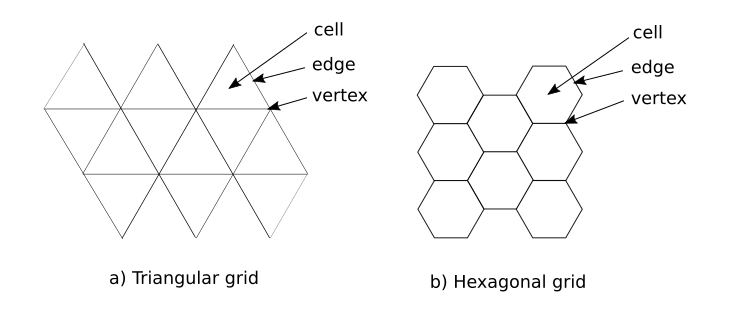
\includegraphics[width=.7\linewidth,natwidth=729,natheight=316]{hgrid.jpg}
  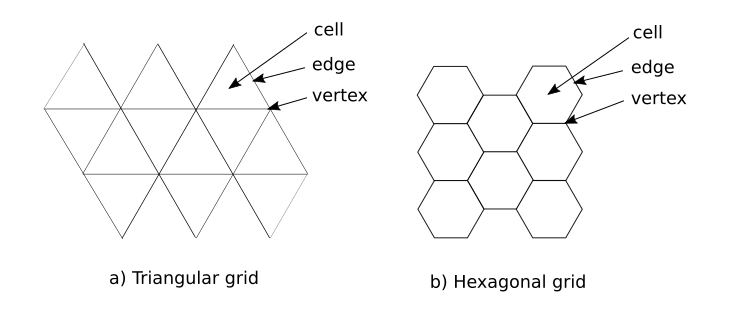
\includegraphics[width=.7\linewidth]{hgrid.jpg}
  \caption{Scope of variables inside the grids}
  \label{fig:grid}
\end{figure}

Larger grids are shown in \Cref{fig:triangulargrid} (and in \Cref{fig:hexagonalgrid}).
There are figures provided that illustrate the neighborhood between data points and for different data localization.

\paragraph{A triangular grid} consists of cells shaped as a triangle (\Cref{fig:grid-triangleempty}).
%It's structure is similar to hexagonal grid.
Values can be located at the centres of the primal grid \Cref{fig:grid-trianglecenter}, and if we connect it to each other, we would see the grid of triangles \Cref{fig:grid-trianglecenter_derived}.
If values are located at the edges (\Cref{fig:grid-triangleedges}) and they are connected with its neighbours, then the grid is given as in \Cref{fig:grid-triangleedges_derived}.
If the values are located at the vertices and they are connected with its neighbours, then the grid is given as in \Cref{fig:grid-trianglevertex}.

\paragraph{Hexagonal grid} consists of cells shaped as a flat topped hexagon (\Cref{fig:grid-hex-empty}).
Two ways can be used to map data to the grid: vertical or horizontal.
Values can be located at the centres of the primal grid (hexagons \Cref{fig:grid-hex-center}), and if we connect it to each other, we would see a grid of triangles \Cref{fig:grid-hex-center_derived}.
If values are located at the edges (\Cref{fig:grid-hex-edges}) and edges are connected with those of the neighbours, then a grid as shown in \Cref{fig:grid-hex-edges_derived} emerges.
If the values are located at the vertices and vertices are connected with those of the neighbours, then a different grid emerges (see \Cref{fig:grid-hex-vertex}).


\subsection{Serialization of Grids}
The abstractions of grids need to be serialized as data structures for the programming languages and for persisting them on storage systems.
In a programming language, regular grids can usually be addressed by n-dimensional arrays.
Thus, a 2D array can be used to store the data of a regular 2D longitude/latitude-based grid.

However, storing irregular grids is not so trivial.
For example, a 1D array can be used to hold the data but then the index has to be determined.
Staying with our 2D example, to map a 2D coordinate onto the 1D array, a mapping between the 2D coordinate and the 1D index has to be found.
One strategy to provide the mapping are space-filling curves.
These curves have the advantage that the indices to some extent preserve locality for points that are  close together -- which can be beneficial, as often operations are conducted on neighbouring data (stencil operations, for example).
A Hilbert curve is an example for one possible enumeration of a multi-dimensional space.

\paragraph{The Hilbert curve}
is a continuous space-filling curve, that helps to represent a grid as an n-dimensional-array of values.
To visualize its behaviour, a 2D grid is shown in \Cref{fig:hilbert-test}.
In 2D, the basic element of the Hilbert curve is a square with one open side.
Every such square has two end-points, and each of these can be the entry-point or the exit-point.
%So, there are four possible varieties of open side.
% ... varieties are completely different mathematical objects ;-P
So, there are four possible variations of an open side.
A first order Hilbert curve consists of one basic element.
It is a 2x2 grid.
The second order Hilbert curve replaces this element by four (smaller) basic elements, which are linked together by three joins (4x4 grid).
Every next order repeats the process by replacing each element by four smaller elements and three joins (8x8 grid).
On the \Cref{fig:hilbert-test} the 5th level Hilbert curve is represented for the 256x256 data, that is mapped to a 32x32 grid.

The characteristics of a Hilbert curve can be extended to more than two dimensions.
The first step in the figure can be wrapped up in as many dimensions as is needed and the points/neighbours will be always saved.


\begin{figure}[!tbp]
 \centering
  \begin{subfigure}[b]{0.4\textwidth}
	 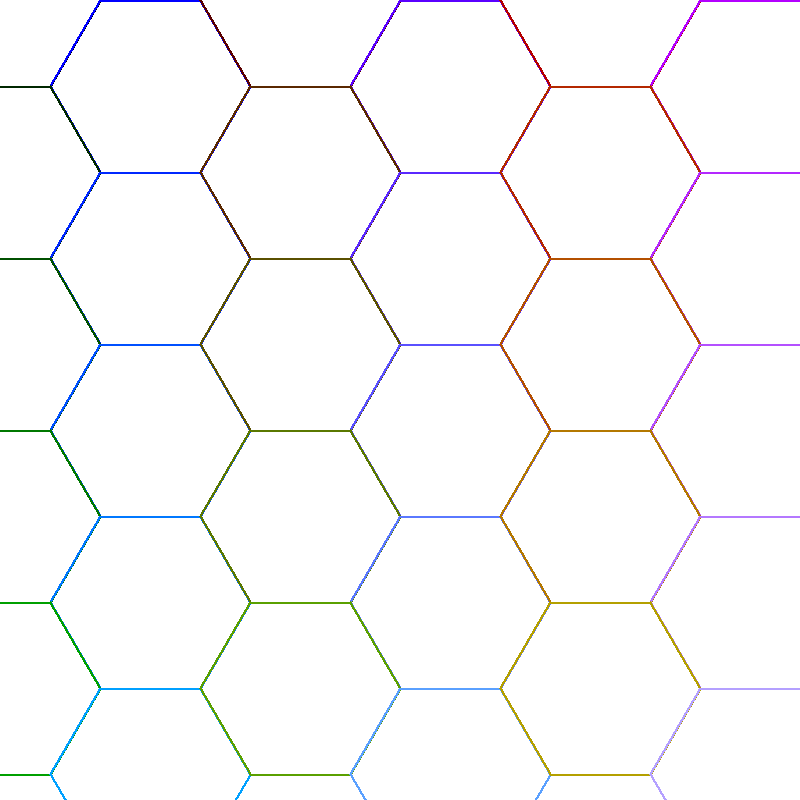
\includegraphics[width=\textwidth] {grid-hex-empty.png}
	 \caption{Empty hexagonal grid}
	 \label{fig:grid-hex-empty}
 \end{subfigure}
 \hfill
 \begin{subfigure}[b]{0.4\textwidth}
	 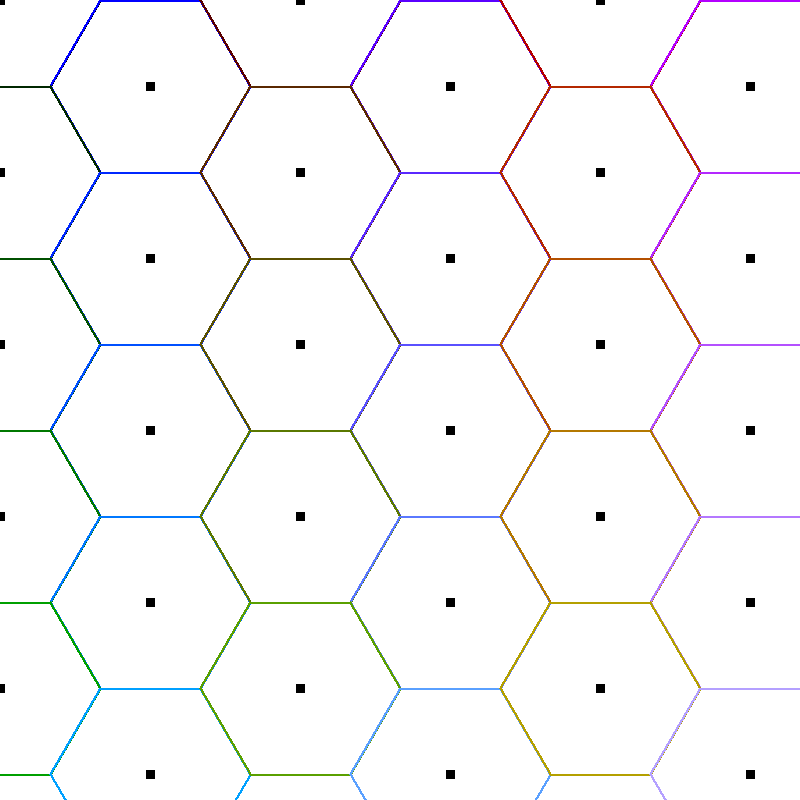
\includegraphics[width=\textwidth] {grid-hex-center.png}
	 \caption{Hexagonal grid with data at the cell centres.}
	 \label{fig:grid-hex-center}
 \end{subfigure}
 \hfill
 \begin{subfigure}[b]{0.4\textwidth}
	 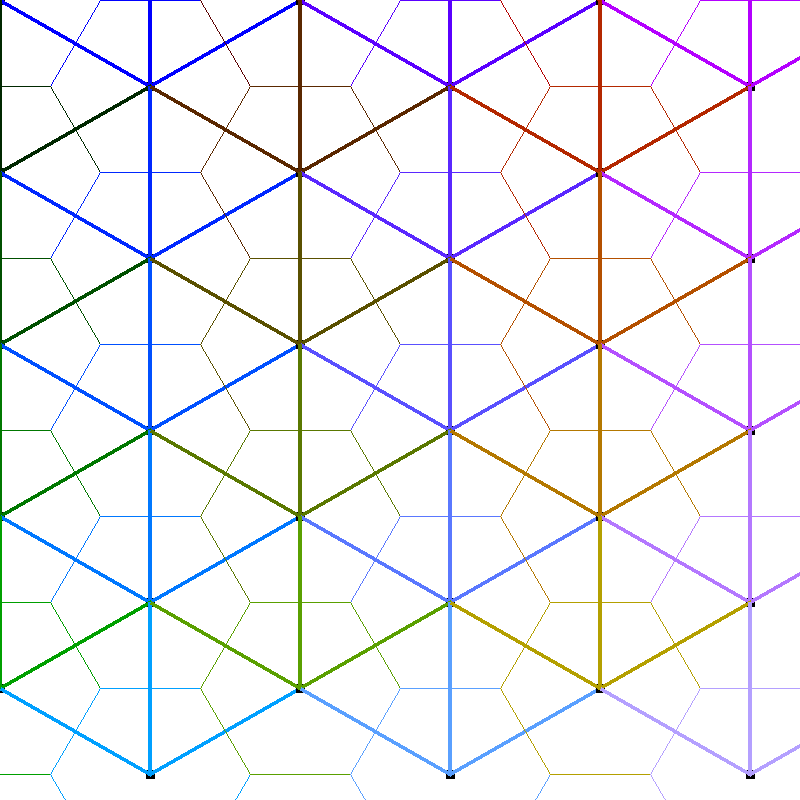
\includegraphics[width=\textwidth] {grid-hex-center_derived.png}
	 \caption{Hexagonal grid with data at the cell's centres, connected neighbours}
	 \label{fig:grid-hex-center_derived}
 \end{subfigure}
 \hfill
 \begin{subfigure}[b]{0.4\textwidth}
	 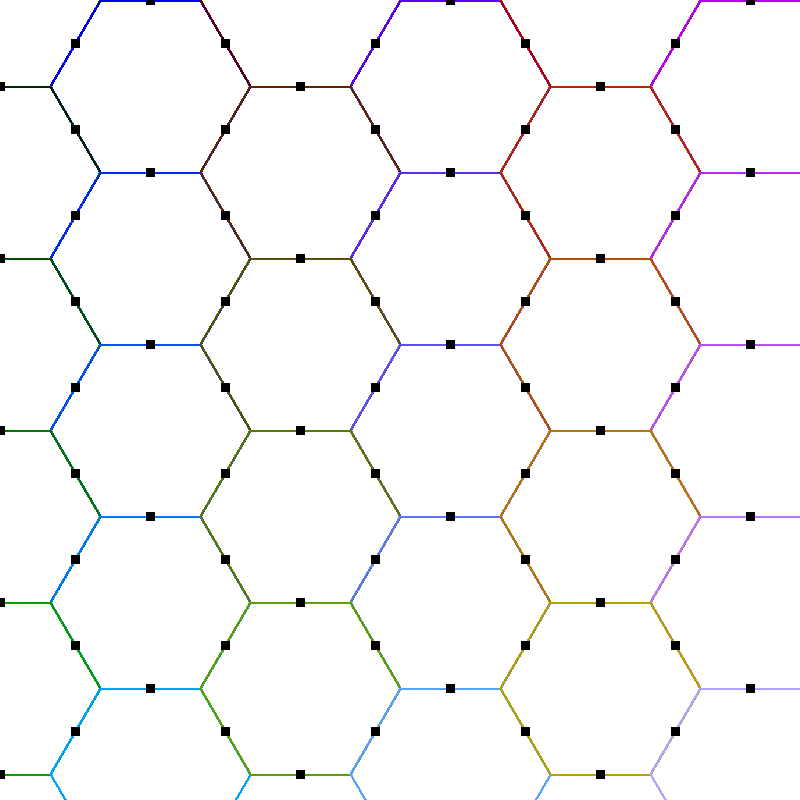
\includegraphics[width=\textwidth] {grid-hex-edges.png}
	 \caption{Hexagonal grid with data on the edges}
	 \label{fig:grid-hex-edges}
 \end{subfigure}
 \hfill
 \begin{subfigure}[b]{0.4\textwidth}
	 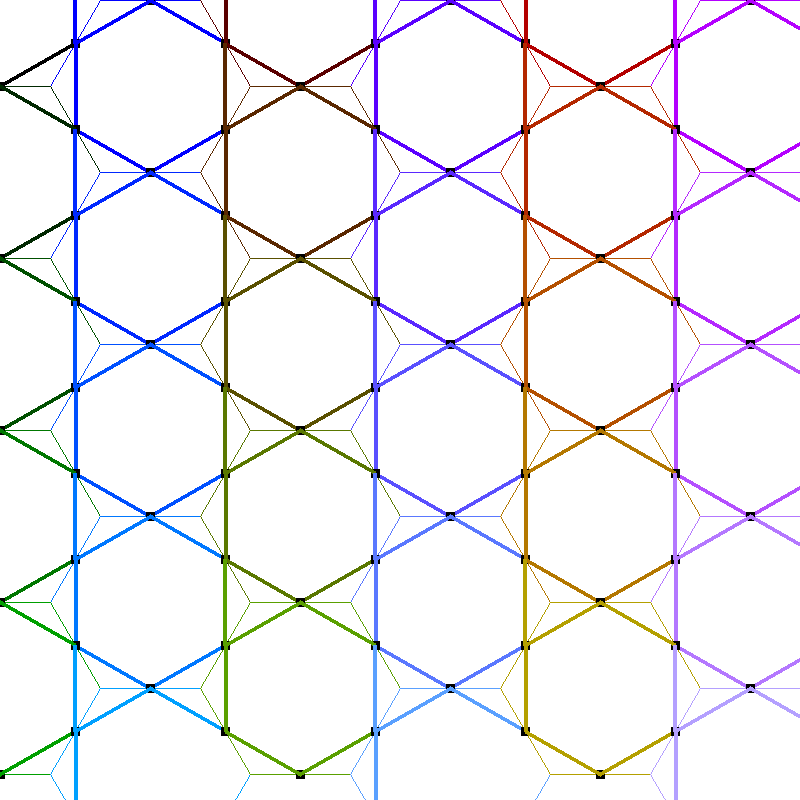
\includegraphics[width=\textwidth] {grid-hex-edges_derived.png}
	 \caption{Hexagonal grid with data on the edges, connected neighbours}
	 \label{fig:grid-hex-edges_derived}
 \end{subfigure}
 \hfill
 \begin{subfigure}[b]{0.4\textwidth}
	 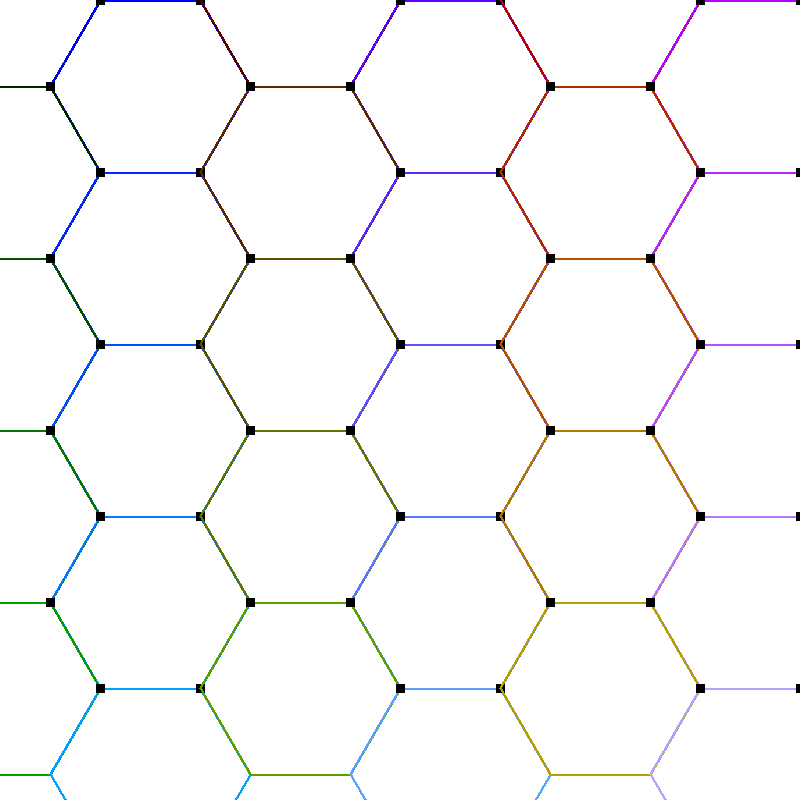
\includegraphics[width=\textwidth] {grid-hex-vertex.png}
	 \caption{Hexagonal grid with data at the vertices / connected neighbours}
	 \label{fig:grid-hex-vertex}
 \end{subfigure}

 \caption{Hexagonal grid}
 \label{fig:hexagonalgrid}
\end{figure}

\begin{figure}[!tbp]
 \centering
  \begin{subfigure}[b]{0.4\textwidth}
	 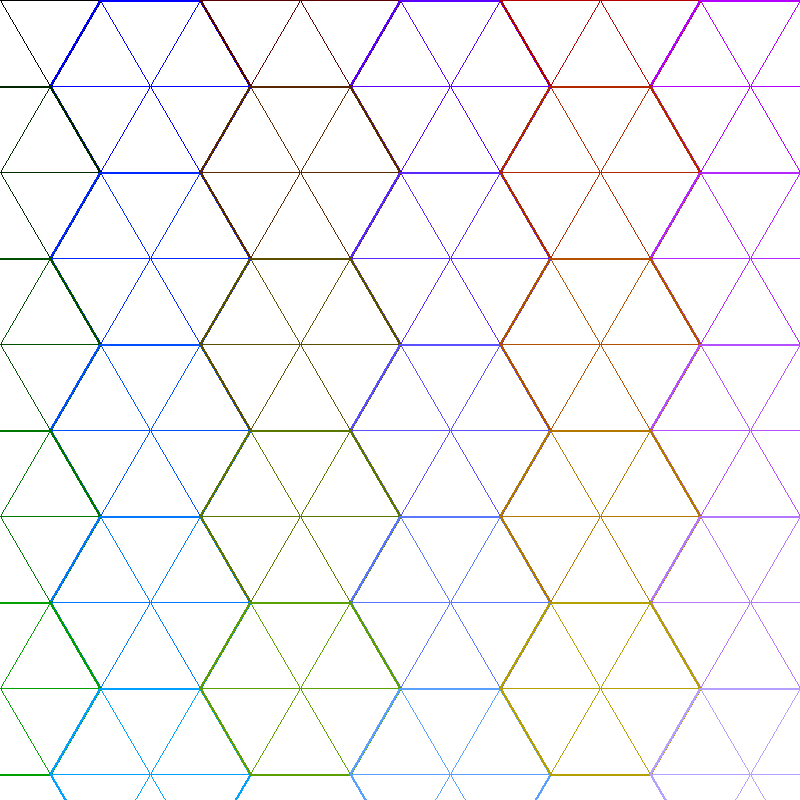
\includegraphics[width=\textwidth] {grid-triangleempty.png}
	 \caption{Empty triangular grid}
	 \label{fig:grid-triangleempty}
 \end{subfigure}
 \hfill
 \begin{subfigure}[b]{0.4\textwidth}
	 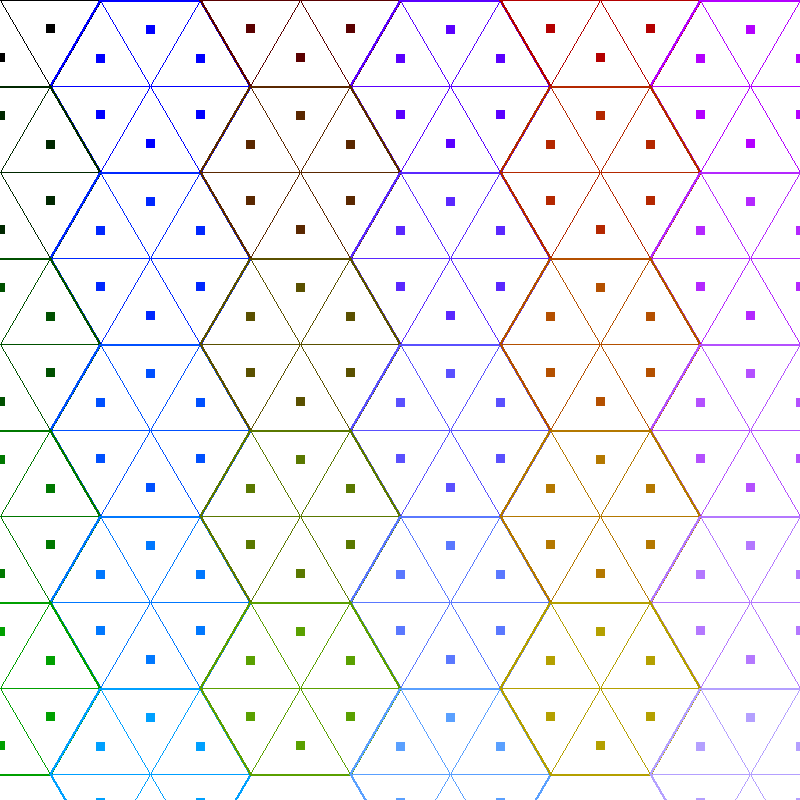
\includegraphics[width=\textwidth] {grid-trianglecenter.png}
	 \caption{Triangular grid with data at the cell centres}
	 \label{fig:grid-trianglecenter}
 \end{subfigure}
 \hfill
 \begin{subfigure}[b]{0.4\textwidth}
	 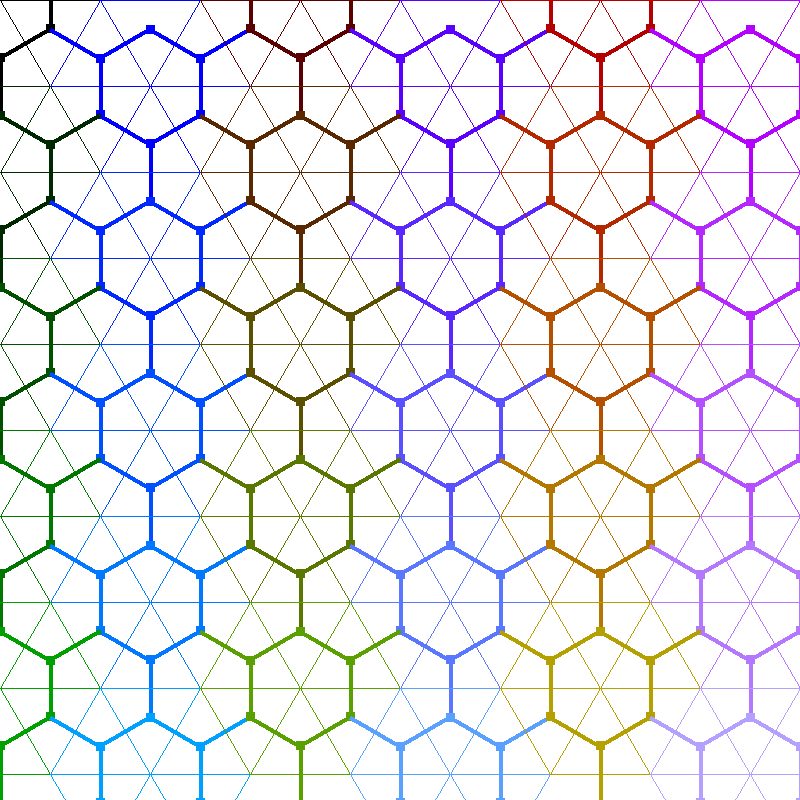
\includegraphics[width=\textwidth] {grid-trianglecenter_derived.png}
	 \caption{Triangular grid with data at the cell centres, connected neighbours}
	 \label{fig:grid-trianglecenter_derived}
 \end{subfigure}
 \hfill
 \begin{subfigure}[b]{0.4\textwidth}
	 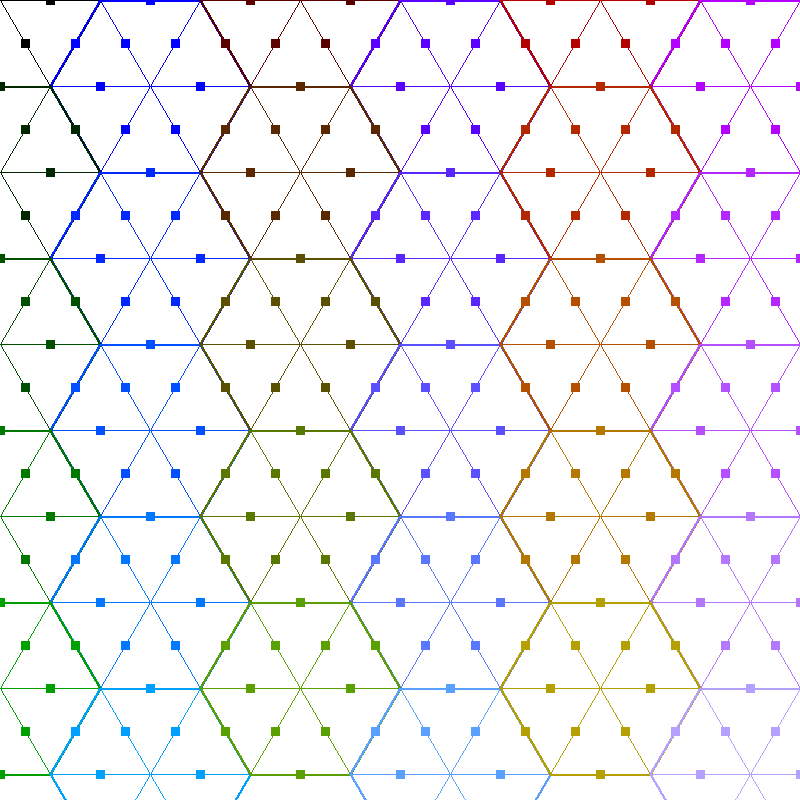
\includegraphics[width=\textwidth] {grid-triangleedges.png}
	 \caption{Triangular grid with data on the edges}
	 \label{fig:grid-triangleedges}
 \end{subfigure}
 \hfill
 \begin{subfigure}[b]{0.4\textwidth}
	 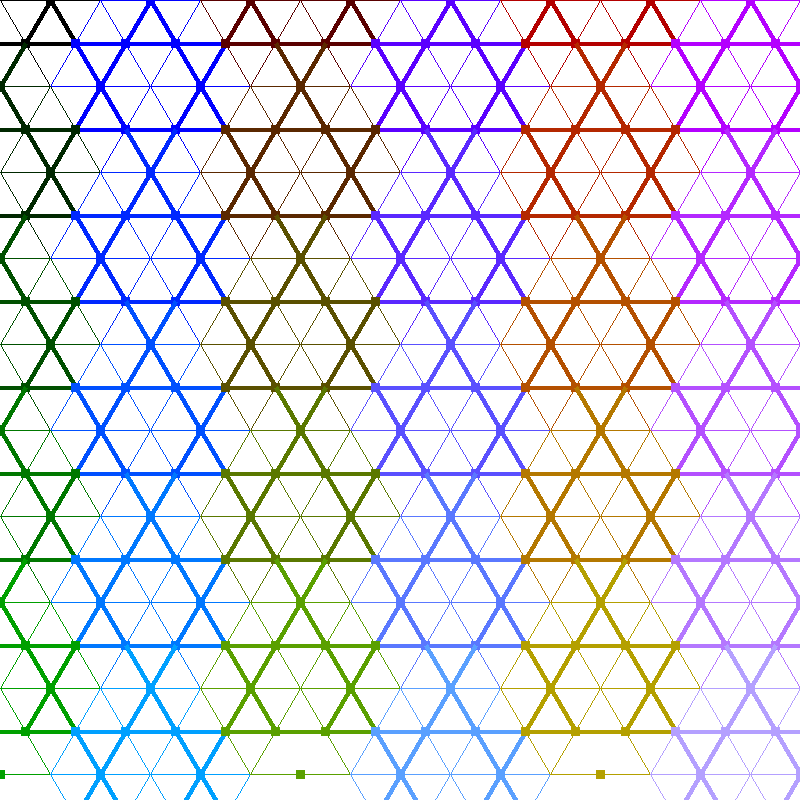
\includegraphics[width=\textwidth] {grid-triangleedges_derived.png}
	 \caption{Triangular grid with data on the edges, connected neighbours}
	 \label{fig:grid-triangleedges_derived}
 \end{subfigure}
 \hfill
 \begin{subfigure}[b]{0.4\textwidth}
	 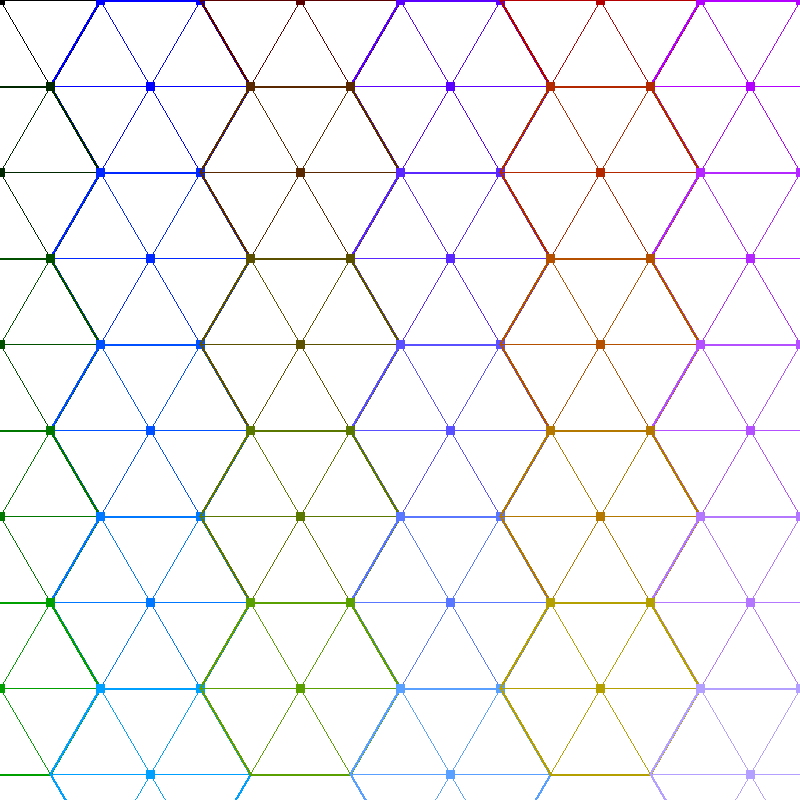
\includegraphics[width=\textwidth] {grid-trianglevertex.png}
	 \caption{Triangular grid with data on the vertices / connected neighbours}
	 \label{fig:grid-trianglevertex}
 \end{subfigure}
 \caption{Triangular grid}
 \label{fig:triangulargrid}
\end{figure}

%\begin{figure}[!tbp]
% \centering
% \adjincludegraphics[trim={0 {.875\height} {.875\width} 0},clip] %{test.png}
% \caption{Hilbert space-filling curve}
% \label{fig:hilbert-test}
%\end{figure}

\begin{figure}[!tbp]
 \centering
 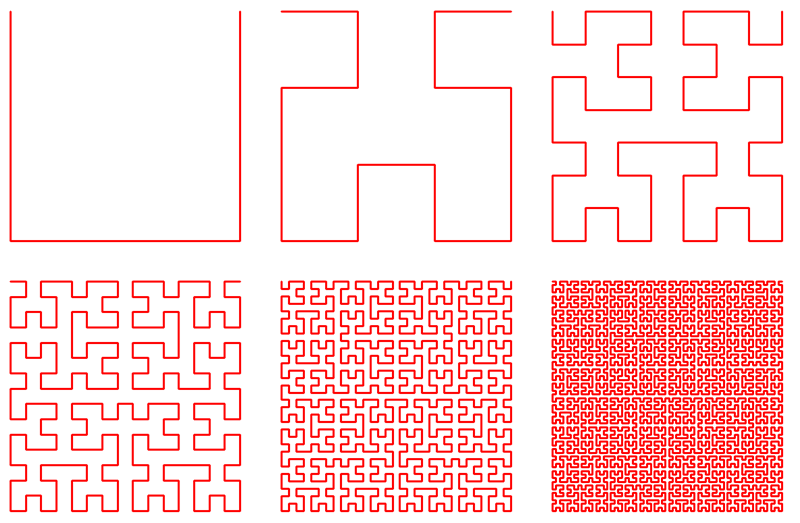
\includegraphics[width=\textwidth] {pattern.png}
 \caption{Hilbert space-filling curve}
 \label{fig:hilbert-test}
\end{figure}

\paragraph{Considerations when serializing to storage systems}

%\todo{@Bryan/Julian: This is where we link the previous material to storage system
%futures and hence relevance to architecture, but it needs to be clearer.}

When serializing a data structure to a storage system, in essence this can be done similarly as in main memory.
The address space exported by the file API of a traditional file system considers the file to be an array of bytes starting from 0.
This is quite similar to the 1D structure from main memory.
However, a general purpose language (GPL) uses variable names to point to the data in this 1D address space.
A GPL offers means to access even multi-dimensional data easily.
The user/programmer does not need to know the specific addresses in memory; addresses are calculated within the execution environment or code of the application.
The main concern here is consecutive or stride access through the array; if the programmer wishes the application to loop through a given dimension of the array, memory locations would be addressed which may not be close to each other in memory, thus leading to cache misses and hence poorer performance.
The generalisation is the stride, which specifies steps through the different dimensions of the array (e.g. incrementing both dimensions of a 2D array, thus walking along the ``diagonal'').
Another special case is where the programmer needs to process the whole array, which would be done most efficiently by stepping through all the memory locations incrementally\footnote{Assuming the whole array is stored in contiguous memory, as it is in these simple examples.},
whereas looping over the dimensions and incrementing them one at a time requires more calculations and may lead to inefficient memory access with cache misses if not done correctly\footnote{Fortran historically stores 2D arrays in column-major order, whereas C and most other languages used in science store data in row-major order.}.

% problematic, as they = ?
%as they are implicitly known by the code and relatively defined by the execution environment of the application in form of stack and heap.

\medskip

When storing data from memory directly on persistent media, then the original source code is necessary to understand this data.
Similarly, the interpretation of the bytes in the data must be same when reading it back, thus, the byte order and size of the datatypes of the machine reading the data must be identical to those of the machine that wrote it.  Floating point numbers must be encoded in the same byte formats.
Since this is not always given, it threatens the longevity of our precious data, by hindering the portability and reusability of the data.

Therefore, portable data formats have been developed that allow serialising and de-serialize data regardless of the machine's architecture.
To allow correct interpretation of a byte array, the library implementing the file format must know the data type that the bytes represent.
This information must be stored besides the actual bytes representing the data to allow later reading and interpretation.
From the user perspective, it is useful to also store further metadata describing the data.
For instance, a name and description of the contained information.
This eases not only debugging but also allows other applications to read and process data.
File formats that contain this kind of semantical and structural metadata are called \textbf{self-describing file formats}.

Developers using a self-describing file format have to use an API to define the metadata.
Such a format may support arbitrary complex data types, which implies that some kind of data description framework must be part of the API for the file format.
See \Cref{sec: data-formats} for more information about data description frameworks.


\section{File formats}
\label{sec: background/file formats}

%\todo{This section is written from a "simulation" only perspective. Need to consider read/write separately, and different aspecs of apects of parallelisation. What about MPI targeted write to OSDS? What about SAFE?}

Generally, parallel scientific applications are designed in such a way, they can solve complicated problems faster when running on a large number of compute nodes.
This is achieved by splitting a global problem into small pieces and distributing them over multiple compute nodes; this is called domain decomposition.
After each node has computed a local solution, they can be aggregated to one global solution.
This approach can decrease time-to-solution considerably.

I/O makes this picture more complicated, especially when data is stored in one single file and is accessed by several processes simultaneously.
In this case, problems can occur, when several processes access the same file region, e.g., two processes can overwrite the data of each other, or inconsistencies can occur when one process reads, while another writes.
Portability is another issue: When transferring data from one platform to another, the contained information should still be accessible and identical.
The purpose of I/O libraries is to hide the complexity from scientists, allowing them to concentrate on their research.



\begin{table}
  \centering
  \begin{tabular}{l|l|l|l}
    Name      & Fullname                   & Version & Developer \\
    \hline
    GRIB1     & GRIdded Binary             & 1       & World Meteorological Organization\\
    GRIB2     & GRIdded Binary             & 2       & World Meteorological Organization\\
    NetCDF3   & Network Common Data Form   & 3.x     & Unidata (UCAR/NCAR)\\
    NetCDF4   & Network Common Data Format & 4.x     & Unidata (UCAR/NCAR\\
    HDF4      & Hierarchical Data Format   & 4.x     & NCSA/NASA\\
    HDF4-EOS2 & HDF4-Earth Observing System & 2       & \\
    HDF5      & Hierarchical Data Format   & 5.x     & NCSA/NASA\\
    HDF5-EOS5 & HDF5-Earth Observing System & 5       & \\
\end{tabular}
\caption{Parallel data formats}
\label{tab:fformats}
\end{table}


Some common file formats are listed in the \Cref{tab:fformats}.
All of these formats are portable (machine independent) and self-describing.
Self-describing means, that files can be examined and read by the appropriate software without the knowledge about the structural details of the file.
The files may include additional information about the data, called ``metadata''.
Often, it is textual information about each variable's contents and units (e.g.,"humidity" and "g/kg") or numerical information describing the coordinates (e.g., time, level, latitude, longitude) that apply to the variables in the file.

GRIB is a record format, NetCDF/HDF/HDF-EOS formats are file formats.
%It is the difference.
In contrast to record format, file formats are bound to format specific rules.
For example, all variable names in NetCDF must be unique.
In HDF, although, variables with the same name are allowed, they must have different paths.
No such rules exist for GRIB.
It is just a collection of records (datasets), which can be appended to the file in any order.

GRIB-1 record (aka, 'message') contains information about two horizontal dimensions (e.g., latitude and longitude) for one time and one level.
GRIB-2 allows each record to contain multiple grids and levels for each time.
However, there are no rules dictating the order of the collection of GRIB records (e.g, records can be in random chronological order).

%Not HPC:
Finally, a file format without parallel I/O support, but still worth to mention, is CSV (comma-separated values).
It is special due to its simplicity, broad acceptance and support by a wide range of applications.
The data is stored as plain text in a table.
Each line of the file is a data record.
Each record consists of one or more fields, that are separated by commas (hence the name).
The CSV file format is not standardized.
There are many implementations that support additional features, e.g., other separators and column names.



\subsection{NetCDF4}

NetCDF4 with Climate Forecast (CF) metadata has evolved to be the de-facto standard format for convenient data access for climate scientists.

It provides a set of features to enable convenient data access, for example, metadata can be used to assign names to variables, set units of measure, label dimensions, and provide other useful information.
Portability allows data movement between different and possibly incompatible platforms, simplifying the exchange of data and facilitating communication between scientists.
The ability to grow and shrink datasets, add new datasets and access small data ranges within datasets expedites the handling of data.
%HPC: Sharable
Shared file access allows keeping the data in the same file, but
unfortunately, it conflicts with performance and efficient usage of state-of-art HPC.
Simultaneous access by several processes causes synchronization overhead which slows down I/O performance (
synchronization is necessary to keep the data consistent).
%Performance: Compression, Chunking

% Relation between HPC imbalance and compression
The rapid development of computational power and storage capacity, and slow development of network bandwidth and I/O performance in the last years resulted in imbalanced HPC systems.
Applications use the increased computational power to create more data.
More data, in turn, requires more costly storage space, higher network bandwidth and sufficient I/O performance on storage nodes.
But due to imbalance, the network and I/O performance are the main bottlenecks.
This can be offset to some extent by using a part of the computational power for compression, adding a little extra latency for the transformation while significantly reducing the amount of data that needs to be transmitted or stored.
% Transition to NetCDF4 and HDF5
However, before considering a compression method for HPC, it is a good idea to take a look at the realization of parallel I/O in modern scientific applications.
Many of them use the NetCDF4 file format, which, in turn, uses HDF5 under the hood.

\subsection{Typical NetCDF Data Mapping}
\label{sec:netcdfDataMapping}
\Cref{lst:NetCDF-data} gives an example for scientific metadata stored in a NetCDF file.
Firstly, between Line 1 and 4, a few dimensions of the multidimensional data are defined.
Here there are longitude, latitude with a fixed size and time with a variable size that allows to be extended (appending from a model).
Then different variables are defined on one or multiple of the dimensions.
The longitude variable provides a measure in “degrees east” and is indexed with the longitude dimension; in that case the variable longitude is a 1D array that contains values for an index between 0-479.
It is allowed to define attributes on variables, this scientific metadata can define the semantics of the data and provide information about the data provenance.
In our example, the unit for longitude is defined in Line\,7.
Multidimensional variables such as \texttt{sund} (Line 17) are defined on a 2D array of values for the longitude and latitude over various timesteps.
The numeric values contain a scale factor and offset that has to be applied when accessing the data; since, here, the data is stored as short values, it should be converted to floating point data in the application.
The \texttt{\_FillValue} indicates a default value for missing data points.

Finally, global attributes such as indicated in Line\,33\, describe that this file is written with the NetCDF-CF schema and its history describes how the data has been derived / extracted from original data.

\begin{tcbcode}[label={lst:NetCDF-data}]{Example NetCDF metadata}
\begin{lstlisting}
dimensions:
	longitude = 480 ;
	latitude = 241 ;
	time = UNLIMITED ; // (1096 currently)
variables:
	float longitude(longitude) ;
		longitude:units = "degrees_east" ;
		longitude:long_name = "longitude" ;
	float latitude(latitude) ;
		latitude:units = "degrees_north" ;
		latitude:long_name = "latitude" ;
	int time(time) ;
		time:units = "hours since 1900-01-01 00:00:0.0" ;
		time:long_name = "time" ;
		time:calendar = "gregorian" ;

	short t2m(time, latitude, longitude) ;
		t2m:scale_factor = 0.00203513170666401 ;
		t2m:add_offset = 257.975148205631 ;
		t2m:_FillValue = -32767s ;
		t2m:missing_value = -32767s ;
		t2m:units = "K" ;
		t2m:long_name = "2 metre temperature" ;
	short sund(time, latitude, longitude) ;
		sund:scale_factor = 0.659209863732776 ;
		sund:add_offset = 21599.6703950681 ;
		sund:_FillValue = -32767s ;
		sund:missing_value = -32767s ;
		sund:units = "s" ;
		sund:long_name = "Sunshine duration" ;

// global attributes:
		:Conventions = "CF-1.0" ;
		:history = "2015-06-03 08:02:17 GMT by grib_to_netcdf-1.13.1: grib_to_netcdf /data/data04/scratch/netcdf-atls14-a562cefde8a29a7288fa0b8b7f9413f7-lFD4z9.target -o /data/data04/scratch/netcdf-atls14-a562cefde8a29a7288fa0b8b7f9413f7-CyGl1B.nc -utime" ;
}
\end{lstlisting}
\end{tcbcode}

% \todo{(BNL) A proper semantic discussion to allow us to introduce "cross file " aggregation would introduce the CF standard here and then discuss the CF aggregation rules and how they need to be supported in the architecture. Agreed !}

%\subsection{SAFE}
% \todo{BNL4BNL: Need to introduce SAFE and describe how much of it is supportable
% within any ESD architecture - leading to a specific requirement in the logical
% view.}


\section{Data Description Frameworks}
\label{sec: data-formats}


Many application developers rely on data description frameworks or libraries to manage data types\footnote{A datatype is a collection of properties, all of which can be stored on storage and which, when taken as a whole, provide complete information for data conversion to or from the datatype.}.
Different libraries and middleware provide mechanisms to describe data using basic types and to construct new ones using dedicated APIs.
Data types are provided as a transparent conversion mechanism between internal representation (as data is represented in memory) and external representation (how data is transmitted over the network or saved to permanent storage).
This section gives an overview of data types provided by different software packages.
Starting from existing middleware and datatype definitions, we will propose a list of basic data types to be supported by the ESD middleware.

%The benefits are manifold and many different projects are available.

%%%%%%%%%%%%%%%%%%%%%%%%%%%%%%%%%%%%%%%%%%%%%%%%%%%%%%%%%%%%%%%%%%%%%%%%%%%%%%%
\subsection{MPI}
The Message Passing Interface supports derived data types for efficient data transfer as well as a short description of file layouts (through file views). MPI defines a set of basic data types (or type class) from which more complex ones can be derived using appropriate data constructor APIs. Basic datatypes in MPI resemble C atomic types as shown in \Cref{table: mpi-types}.

\clearpage

\begin{longtable}{|>{\centering\arraybackslash} m{5.5cm} | >{\centering\arraybackslash} m{6cm} |}\hline\hline
        \cellHeader Datatype                  & \cellHeader Description                                                               \\ \hline
        \small \texttt{MPI\_CHAR}                     & \small this is the traditional ASCII character that is numbered by integers between 0 and 127 \\ \hline
        \small \texttt{MPI\_WCHAR}                    & \small this is a wide character, e.g., a 16-bit character such as a Chinese ideogram          \\ \hline
        \small \texttt{MPI\_SHORT}                    & \small this is a 16-bit integer between -32,768 and 32,767                                    \\ \hline
        \small \texttt{MPI\_INT}                      & \small this is a 32-bit integer between -2,147,483,648 and 2,147,483,647                      \\ \hline
        \small \texttt{MPI\_LONG}                     & \small this is the same as MPI\_INT on IA32                                                   \\ \hline
        \small \texttt{MPI\_LONG\_LONG\_INT}          & \small this is a 64-bit long signed integer, i.e., %
                                                        an integer number between -9,223,372,036,854,775,808 and 9,223,372,036,854,775,807            \\ \hline
        \small \texttt{MPI\_LONG\_LONG}               & \small same as MPI\_LONG\_LONG\_INT                                                           \\ \hline
        \small \texttt{MPI\_SIGNED\_CHAR}             & \small same as MPI\_CHAR                                                                      \\ \hline
        \small \texttt{MPI\_UNSIGNED\_CHAR}           & \small this is the extended character numbered by integers between 0 and 255                  \\ \hline
        \small \texttt{MPI\_UNSIGNED\_SHORT}          & \small this is a 16-bit positive integer between 0 and 65,535                                 \\ \hline
        \small \texttt{MPI\_UNSIGNED\_LONG}           & \small this is the same as MPI\_UNSIGNED on IA32                                              \\ \hline
        \small \texttt{MPI\_UNSIGNED}                 & \small this is a 32-bit unsigned integer, i.e., a number between 0 and 4,294,967,295          \\ \hline
        \small \texttt{MPI\_FLOAT}                    & \small this is a single precision, 32-bit long floating point number                          \\ \hline
        \small \texttt{MPI\_DOUBLE}                   & \small this is a double precision, 64-bit long floating point number                          \\ \hline
        \small \texttt{MPI\_LONG\_DOUBLE}             & \small this is a quadruple precision, 128-bit long floating point number                      \\ \hline
        \small \texttt{MPI\_C\_COMPLEX}               & \small this is a complex float                                                                \\ \hline
        \small \texttt{MPI\_C\_FLOAT\_COMPLEX}        & \small same as MPI\_C\_COMPLEX                                                                \\ \hline
        \small \texttt{MPI\_C\_DOUBLE\_COMPLEX}       & \small this is a complex double                                                               \\ \hline
        \small \texttt{MPI\_C\_LONG\_DOUBLE\_COMPLEX} & \small this is a long double complex                                                          \\ \hline
        \small \texttt{MPI\_C\_BOOL}                  & \small this is a \_Bool                                                                       \\ \hline
        \small \texttt{MPI\_INT8\_T}                  & \small this is a 8-bit integer                                                                \\ \hline
        \small \texttt{MPI\_INT16\_T}                 & \small this is a 16-bit integer                                                               \\ \hline
        \small \texttt{MPI\_INT32\_T}                 & \small this is a 32-bit integer                                                               \\ \hline
        \small \texttt{MPI\_INT64\_T}                 & \small this is a 64-bit integer                                                               \\ \hline
        \small \texttt{MPI\_UINT8\_T}                 & \small this is a 8-bit unsigned integer                                                       \\ \hline
        \small \texttt{MPI\_UINT16\_T}                & \small this is a 16-bit unsigned integer                                                      \\ \hline
        \small \texttt{MPI\_UINT32\_T}                & \small this is a 32-bit unsigned integer                                                      \\ \hline
        \small \texttt{MPI\_UINT64\_T}                & \small this is a 64-bit unsigned integer                                                      \\ \hline
        \small \texttt{MPI\_BYTE}                     & \small this is an 8-bit positive integer                                                      \\ \hline
        \small \texttt{MPI\_PACKED}                   & -                                                                                             \\ \hline
        \caption{MPI Datatypes}
        \label{table: mpi-types}
\end{longtable}

Data types from Table~\ref{table: mpi-types} can be used in combination with the constructor APIs shown in Table~\ref{table: mpi-constr} to build more complex derived data types.

\begin{longtable}{|>{\centering\arraybackslash} m{5.5cm} | >{\centering\arraybackslash} m{6cm} |}\hline\hline
        \cellHeader Datatype Constructor           & \cellHeader Description                               \\ \hline
        \small \texttt{MPI\_Type\_create\_hindexed}        & \small create an indexed datatype with displacement in bytes  \\ \hline
        \small \texttt{MPI\_Type\_create\_hindexed\_block} & \small create an hindexed datatype with constant-sized blocks \\ \hline
        \small \texttt{MPI\_Type\_create\_indexed\_block}  & \small create an indexed datatype with constant-sized blocks  \\ \hline
        \small \texttt{MPI\_Type\_create\_keyval}          & \small create an attribute keyval for MPI data types           \\ \hline
        \small \texttt{MPI\_Type\_create\_hvector}         & \small create a datatype with constant stride given in bytes  \\ \hline
        \small \texttt{MPI\_Type\_create\_struct}          & \small create a MPI datatype from a general set of data types, %
                                                             displacements and block sizes                                 \\ \hline
        \small \texttt{MPI\_Type\_create\_darray}          & \small create a datatype representing a distributed array     \\ \hline
        \small \texttt{MPI\_Type\_create\_resized}         & \small create a datatype with a new lower bound and extent %
                                                             from an existing datatype                                     \\ \hline
        \small \texttt{MPI\_Type\_create\_subarray}        & \small create a datatype for a subarray of a regular, %
                                                             multidimensional array                                        \\ \hline
        \small \texttt{MPI\_Type\_contiguous}              & \small create a contiguous datatype                           \\ \hline
        \caption{MPI Derived Datatypes Constructors}
        \label{table: mpi-constr}
\end{longtable}

Before they can be used, MPI derived data types (created using the constructors in Table~\ref{table: mpi-constr}) have to be committed to memory using the \texttt{MPI\_Type\_commit} interface.
Similarly, when no longer needed, derived data types can be freed using the \texttt{MPI\_Type\_free} interface.
Unlike data format libraries, MPI does not provide any permanent data representation (MPI-IO can only read/write binary data), therefore derived data types are not used to store any specific data format on stable storage and are instead used only for data transfers or file layout descriptions.

Example code for defining a derived data structure for a structure is shown in \Cref{lst:mpi-struct}.
The structure is defined in Lines 5-9.
The function in Lines 12-22 registers this datatype in MPI.
It is required to define the beginning and end of each array, its type and size.
Once a datatype is defined, it can be used as memory type in subsequent operations.
In this example, one process sends this datatype to another process (Line 38 and Line 45).

Since MPI data types were initially designed for computation and, thus, to define memory regions, they do not offer a way to name the data structures.

\begin{tcbcode}[label={lst:mpi-struct}]{Example construction of an MPI datatype for a structure}
\begin{lstlisting}[language=c++,morekeywords={{student_t}}]
#include <stdio.h>
#include <string.h>
#include <mpi.h>

typedef struct student_t_s {
    int id[2];
    float grade[5];
    char name[20];
} student_t;

/* create a type for the struct student_t */
void create_student_datatype(MPI_Datatype * mpi_student_type){
    int   blocklengths[3] = {2, 5, 20};
    MPI_Datatype types[3] = {MPI_INT, MPI_FLOAT, MPI_CHAR};
    MPI_Aint     offsets[3];

    offsets[0] = offsetof(student_t, id) ;
    offsets[1] = offsetof(student_t, grade);
    offsets[2] = offsetof(student_t, name);
    MPI_Type_create_struct(3, blocklengths, offsets, types, mpi_student_type);
    MPI_Type_commit(mpi_student_type);
}

int main(int argc, char **argv) {
    const int tag = 4711;
    int size, rank;

    MPI_Init(&argc, &argv);
    MPI_Comm_size(MPI_COMM_WORLD, &size);
    MPI_Comm_rank(MPI_COMM_WORLD, &rank);

    MPI_Datatype mpi_student_type;
    create_student_datatype(& mpi_student_type);

    if (rank == 0) {
        student_t send = {{1, 2},  {1.0, 2.0, 1.7, 2.0, 1.7},  "Nina Musterfrau"};
        const int target_rank = 1;
        MPI_Send(&send,   1, mpi_student_type, target_rank, tag, MPI_COMM_WORLD);
    }
    if (rank == 1) {
        MPI_Status status;
        const int src=0;
        student_t recv;
        memset(& recv, 0, sizeof(student_t));
        MPI_Recv(&recv,   1, mpi_student_type, src, tag, MPI_COMM_WORLD, &status);
        printf("Rank %d: Received: id = %d grade = %f student = %s\n", rank, recv.id[0], recv.grade[0], recv.name);
    }

    MPI_Type_free(&mpi_student_type);
    MPI_Finalize();

    return 0;
}
\end{lstlisting}
\end{tcbcode}



%%%%%%%%%%%%%%%%%%%%%%%%%%%%%%%%%%%%%%%%%%%%%%%%%%%%%%%%%%%%%%%%%%%%%%%%%%%%%%%
\subsection{HDF5}

%The hierarchical data format is...

%\begin{quotation}
%\itshape
HDF5 is a data model, library, and file format for storing and managing data. It supports an unlimited variety of data types and is designed for flexible and efficient I/O and high volume and complex data.
HDF5 is portable and is extensible, allowing applications to evolve in their use of HDF5.
The HDF5 Technology suite includes tools and applications for managing, manipulating, viewing, and analysing data in the HDF5 format. Like MPI, HDF5 also supports its own basic (native) data types reported in \Cref{table: hdf5-types}.
%\end{quotation}

\begin{longtable}{|>{\centering\arraybackslash} m{5.5cm} | >{\centering\arraybackslash} m{6cm} |}\hline\hline
        \cellHeader Datatype        & \cellHeader Corresponding C Type                  \\ \hline
        \small \texttt{H5\_NATIVE\_CHAR}    & \small \texttt{char}                                      \\ \hline
        \small \texttt{H5\_NATIVE\_SCHAR}   & \small \texttt{signed char}                               \\ \hline
        \small \texttt{H5\_NATIVE\_UCHAR}   & \small \texttt{unsigned char}                             \\ \hline
        \small \texttt{H5\_NATIVE\_SHORT}   & \small \texttt{short}                                     \\ \hline
        \small \texttt{H5\_NATIVE\_USHORT}  & \small \texttt{unsigned short}                            \\ \hline
        \small \texttt{H5\_NATIVE\_INT}     & \small \texttt{int}                                       \\ \hline
        \small \texttt{H5\_NATIVE\_UINT}    & \small \texttt{unsigned int}                              \\ \hline
        \small \texttt{H5\_NATIVE\_LONG}    & \small \texttt{long}                                      \\ \hline
        \small \texttt{H5\_NATIVE\_ULONG}   & \small \texttt{unsigned long}                             \\ \hline
        \small \texttt{H5\_NATIVE\_LLONG}   & \small \texttt{long long}                                 \\ \hline
        \small \texttt{H5\_NATIVE\_ULLONG}  & \small \texttt{unsigned long long}                        \\ \hline
        \small \texttt{H5\_NATIVE\_FLOAT}   & \small \texttt{float}                                     \\ \hline
        \small \texttt{H5\_NATIVE\_DOUBLE}  & \small \texttt{double}                                    \\ \hline
        \small \texttt{H5\_NATIVE\_LDOUBLE} & \small \texttt{long double}                               \\ \hline
        \small \texttt{H5\_NATIVE\_B8}      & \small 8-bit unsigned integer or 8-bit buffer in memory   \\ \hline
        \small \texttt{H5\_NATIVE\_B16}     & \small 16-bit unsigned integer or 16-bit buffer in memory \\ \hline
        \small \texttt{H5\_NATIVE\_B32}     & \small 32-bit unsigned integer or 32-bit buffer in memory \\ \hline
        \small \texttt{H5\_NATIVE\_B64}     & \small 64-bit unsigned integer or 64-bit buffer in memory \\ \hline
        %\small \texttt{H5\_NATIVE\_OPAQUE} & \small \\ \hline
        \small \texttt{H5\_NATIVE\_HADDR}   & \small \texttt{haddr\_t}                                  \\ \hline
        \small \texttt{H5\_NATIVE\_HSIZE}   & \small \texttt{hsize\_t}                                  \\ \hline
        \small \texttt{H5\_NATIVE\_HSSIZE}  & \small \texttt{hssize\_t}                                 \\ \hline
        \small \texttt{H5\_NATIVE\_HERR}    & \small \texttt{herr\_t}                                   \\ \hline
        \small \texttt{H5\_NATIVE\_HBOOL}   & \small \texttt{hbool\_t}                                  \\ \hline
        \caption{HDF5 Native Datatypes}
        \label{table: hdf5-types}
\end{longtable}

Besides the native data types, the library also provides so-called standard data types, architecture specific data types (e.g., for i386), IEEE floating point data types, and others.
Data types can be built or modified starting from the native set of data types using the constructors as listed in \Cref{table: hdf5-constr}.

HDF5 constructs allow the user a fine-grained definition of arbitrary data types.
Indeed, HDF5 allows the user to build a user-defined datatype starting from a native datatype (by copying the native type) and then change datatype characteristics like the sign, precision, etc., using the supported datatype constructor API.
However, since these user-defined data types often have no direct representation of available hardware, this can lead to performance issues.

\clearpage

\begin{longtable}{|>{\centering\arraybackslash} m{5.5cm} | >{\centering\arraybackslash} m{6cm} |}\hline\hline
        \cellHeader Datatype Constructor & \cellHeader Description \\ \hline
        \small \texttt{H5Tcreate}                & \small Creates a new datatype of the specified class with the specified number of bytes. This function is used only with the following datatype classes: %
                                                   H5T\_COMPOUND, H5T\_OPAQUE, H5T\_ENUM, H5T\_STRING. %
                                                   Other data types, including integer and floating-point data types, are %
                                                   typically created by using H5Tcopy to copy and modify %
                                                   a predefined datatype                                                               \\ \hline
        \small \texttt{H5Tvlen\_create}          & \small Creates a new one-dimensional array datatype of variable-length (VL) with %
                                                   the base datatype. The base type specified for the VL datatype can be any HDF5 %
                                                   datatype, including another VL datatype, a compound datatype, or an atomic datatype \\ \hline
        \small \texttt{H5Tarray\_create}         & \small Creates a new multidimensional array datatype object                         \\ \hline
        \small \texttt{H5Tenum\_create}          & \small Creates a new enumeration datatype based on the specified base datatype, %
                                                   dtype\_id, which must be an integer datatype                                        \\ \hline
        \small \texttt{H5Tcopy}                  & \small Copies an existing datatype. The returned type is always transient and unlocked. A native datatype can be copied and modified using other APIs %
                                                   (e.g. changing the precision)                                                       \\ \hline
        \small \texttt{H5Tset\_precision}        & \small Sets the precision of an atomic datatype. The precision is the number of significant bits                                                                    \\ \hline
        \small \texttt{H5Tset\_sign}             & \small Sets the sign property for an integer type. The sign can be unsigned or two's complement                                                                    \\ \hline
        \small \texttt{H5Tset\_size}             & \small Sets the total size in bytes for a datatype                                  \\ \hline
        \small \texttt{H5Tset\_order}            & \small Sets the byte order of a datatype (big endian or little endian)              \\ \hline
        \small \texttt{H5Tset\_offset}           & \small Sets the bit offset of the first significant bit                             \\ \hline
        \small \texttt{H5Tset\_fields}           & \small Sets the locations and sizes of the various floating-point bit fields. The field positions are bit positions in the significant region of the datatype. Bits are numbered with the least significant bit number zero                        \\ \hline
        \caption{HDF5 Data types Constructors}
        \label{table: hdf5-constr}
\end{longtable}

\clearpage

%%%%%%%%%%%%%%%%%%%%%%%%%%%%%%%%%%%%%%%%%%%%%%%%%%%%%%%%%%%%%%%%%%%%%%%%%%%%%%%
\subsection{NetCDF}

NetCDF is a crucial and popular alternative within the climate community. NetCDF provides a set of software libraries and self-describing, machine-independent, data formats that support the creation, access, and sharing of array-oriented scientific data.
In version 4 of the library (NetCDF4), the used binary file representation is HDF5. Like MPI and HDF5, NetCDF also defines its own set of atomic data types as shown in \Cref{table: netcdf-types}.
%\end{quotation}

\begin{table}
\centering
\begin{tabular}{|>{\centering\arraybackslash} m{5.5cm} | >{\centering\arraybackslash} m{6cm} |}\hline\hline
        \cellHeader Datatype & \cellHeader Description         \\ \hline
        \small \texttt{NC\_BYTE}     & \small 8-bit signed integer             \\ \hline
        \small \texttt{NC\_UBYTE}    & \small 8-bit unsigned integer           \\ \hline
        \small \texttt{NC\_CHAR}     & \small 8-bit character byte             \\ \hline
        \small \texttt{NC\_SHORT}    & \small 16-bit signed integer            \\ \hline
        \small \texttt{NC\_USHORT}   & \small 16-bit unsigned integer          \\ \hline
        \small \texttt{NC\_INT}      & \small 32-bit signed integer            \\ \hline
        \small \texttt{NC\_UINT}     & \small 32-bit unsigned integer          \\ \hline
        \small \texttt{NC\_INT64}    & \small 64-bit signed integer            \\ \hline
        \small \texttt{NC\_UINT64}   & \small 64-bit unsigned integer          \\ \hline
        \small \texttt{NC\_FLOAT}    & \small 32-bit floating point            \\ \hline
        \small \texttt{NC\_DOUBLE}   & \small 64-bit floating point            \\ \hline
        \small \texttt{NC\_STRING}   & \small variable length character string \\ \hline
\end{tabular}
        \caption{netCDF Atomic External Datatypes}
        \label{table: netcdf-types}
\end{table}


Similarly, to HDF5 and MPI, in addition to the atomic types, the user can define their own types. NetCDF supports four different user-defined types:
%
\begin{enumerate}
        \item \textbf{Compound}: are a collection of types (either user defined or atomic)
        \item \textbf{Variable Length Arrays}: are used to store non-uniform arrays
        \item \textbf{Opaque}: only contain the size of each element and no datatype information
        \item \textbf{Enum}: like an enumeration in C
\end{enumerate}

Once types are constructed, variables of the new type can be instantiated with \texttt{nc\_def\_var}. Data can be written to the new variable using  \texttt{nc\_put\_var1}, \texttt{nc\_put\_var}, \texttt{nc\_put\_vara}, or \texttt{nc\_put\_vars}. Data can be read from the new variable with \texttt{nc\_get\_var1}, \texttt{nc\_get\_var}, \texttt{nc\_get\_vara}, or \texttt{nc\_get\_vars}.
Finally, new attributes can be added to the variable using nc\_put\_att, and existing attributes can be accessed from the variable using \texttt{nc\_get\_att}.


\medskip

Table~\ref{table: netcdf-constr} shows the constructors provided to build user-defined data types.

\begin{longtable}{|>{\centering\arraybackslash} m{1.7cm} | >{\centering\arraybackslash} m{4.5cm} | >{\centering\arraybackslash} m{5cm} |}\hline\hline
        \cellHeader Type & \cellHeader Constructor & \cellHeader Description \\ \hline
        \multirow{4}{1.7cm}{\centering \small Compound} %
                                             & \small \texttt{nc\_def\_compound}              & \small create a compound datatype                     \\ \cline{2-3}
                                             & \small \texttt{nc\_insert\_compound}           & \small insert a name field into a compound datatype   \\ \cline{2-3}
                                             & \small \texttt{nc\_insert\_array\_compound}    & \small insert an array field into a compound datatype \\ \cline{2-3}
                                             & \small \texttt{nc\_inq\_\{compound,name,...\}} & \small learn information about a compound datatype    \\ \hline
        \multirow{3}{1.7cm}{\centering \small Variable Length Array}%
                                             & \small \texttt{nc\_def\_vlen}                  & \small create a variable length array                 \\ \cline{2-3}
                                             & \small \texttt{nc\_inq\_vlen}                  & \small learn about a variable length array            \\ \cline{2-3}
                                             & \small \texttt{nc\_free\_vlen}                 & \small release memory from a variable length array    \\ \hline
        \multirow{2}{1.7cm}{\centering \small Opaque} %
                                             & \small \texttt{nc\_def\_opaque}                & \small create an opaque datatype                      \\ \cline{2-3}
                                             & \small \texttt{nc\_inq\_opaque}                & \small learn about an opaque datatype                 \\ \hline
        \multirow{3}{1.7cm}{\centering \small Enum} %
                                             & \small \texttt{nc\_def\_enum}                  & \small create an enum datatype                        \\ \cline{2-3}
                                             & \small \texttt{nc\_insert\_enum}               & \small insert a named member into an enum datatype    \\ \cline{2-3}
                                             & \small \texttt{nc\_inq\_\{enum,...\}}          & \small learn information about an enum datatype       \\ \hline
        \caption{NetCDF Datatypes Constructors}
        \label{table: netcdf-constr}
\end{longtable}
\newpage




%%%%%%%%%%%%%%%%%%%%%%%%%%%%%%%%%%%%%%%%%%%%%%%%%%%%%%%%%%%%%%%%%%%%%%%%%%%%%%%
\subsection{GRIB}
%unlike HDF5, NetCDF or MPI grib specifies messages which can contain certain data sections

%GRIB is widely used
%and standardised by \cite{WMO}
GRIB is a library and data format commonly used in weather applications.
It differs from previously described libraries in the sense that it does not define datatypes that can be used to store a wide range of different data.
Instead, GRIB very clearly defines the sections of every -- so-called -- message which is the unit sent across a network link or written to permanent storage.
Every message in GRIB has different sections, each of which contains some information.
GRIB defines the units that can be represented in every message and thus does not explicitly need datatypes to represent them.
But a library supporting these formats needs to know the mapping from a message type to the contained data fields and their data types.
In that sense, GRIB is not a self-describing file format but requires a code to define the standardised content.
GRIB messages contain 32-bit integers that can be scaled using a predefined data packing schema. The scaling factor is stored along with the data inside the message.


%%%%%%%%%%%%%%%%%%%%%%%%%%%%%%%%%%%%%%%%%%%%%%%%%%%%%%%%%%%%%%%%%%%%%%%%%%%%%%%
\section{Storage Systems}
\label{sec: background/storage systems}

This section introduces interesting storage systems, in particular, software concepts.
With ESD, we focus on HPC. However, other fields are very active in the creation of storage systems with embedded processing engines.
Since we use some low-level concepts which are exploited by existing software products, we introduce these solutions briefly.
ESD directly uses some of the listed systems.

\subsection{WOS}
\label{WOS background}

DDN (Data Direct Network) WOS (Web object scaler)\footnote{\url{http://www.ddn.com/products/object-storage-web-object-scaler-wos/}} represents an object storage solution able to manage files as ``objects''.

It offers a simple and effective way to manage data stored in the cloud through an ease administration interface and IP based direct connection to the nodes.
WOS architecture is natively geographically agnostic, and this represents one of the main features of the product: nodes can be deployed anywhere, and the access to data which they host is guaranteed by Internet Protocol (IP) connectivity.
In this sense, all the nodes which form the cloud work together to create an aggregated pool of storage space.

WOS relies on the following features and concepts:
\begin{itemize}
\item \textbf{nodes, zones and cloud}: nodes represent the addressable elements of the architecture; they participate in the cloud environment providing their storage space and computational power.
The nodes are connected to the WOS cloud through a preferably high-speed internet connection.
Multiple nodes form a zone which collects nodes with a specific policy. The WOS system is able to balance the load among the nodes within a zone automatically.
The pool of the zones forms the entire WOS cloud, and the membership of a common network guarantees the communication in the cloud.
\item \textbf{policy}: the administrator defines different rules which determine the object distribution. It is important to highlight that files + metadata + policy form an Object.
\item \textbf{object:} an object is formed by multiple elements managed by WOS as a single entity. For instance, an object could be a file stored in the WOS cloud or a group of them.
\item \textbf{Object ID (OID)}: An OID uniquely identifies an object (and its replicas, if any). The OID has to be provided to the WOS system for allowing the addressing and retrieving of the related object.
\end{itemize}
In addition to these, WOS supports the definition of metadata by the users in the form of key-value pairs and multiple replicas for each object (managed by the policy rules).

WOS cloud is an excellent solution to take into account to manage data in environments which present particular features or challenges that could affect the traditional architectures based on common file-systems and storage solutions.
For example, this cloud can be successfully applied when data sets are too large for a single file system and, so, they need to be stored on multiple sites or, on the contrary, there are large quantities of files which are very small.
Other examples are systems that present high rates of file read, write and/or file deletion or if users want a small system to start with the possibility to easily scale up.
The only requirements of a WOS installation are related to the connection between the nodes: nodes must be interconnected through a network (LAN or WAN or a combination of them) and must be able to communicate using the TCP/IP protocol.
The network between the nodes should be stable and reliable (anyway WOS system are able to recover the regular operational activity after a network outages), fast (multiple Gigabit ports are preferred or 10 Gigabit Ethernet connections) and low-latency (which is an important aspect especially for TCP/IP connections so using low-latency appliances will guarantee the best results).

The WOS Core relies on three main services and an instance of each service is installed on each node that forms the WOS cluster. These services are:
\begin{itemize}
\item The\textbf{Management Tuning Service (MTS)} which has the task to control the administration and configuration functions.
The master node hosts the primary MTS while the other nodes host an instance of this service.

\item The \textbf{wosnode} which is hosted on each node of the cluster. It manages and controls all the I/O operations to the connected devices. The WOS node operates only on the local node also in the case the MTS goes down to improve performance and reliability.

\item The \textbf{wosrest} represents the service which provides the REST (Representational State Transfer) interface. An application that accesses the WOS cluster over the network interact with the node through this service and the REST interface.
\end{itemize}

\textbf{The WOS API}

WOS architecture provides several APIs for connecting an application to the cluster, manages the objects and the related metadata.
Specifically, WOS provides API for C++, JAVA and Python languages.
In addition, it provides an HTTP Restful interface.
It is not allowed to modified objects so each object can be written only once, read many times and eventually deleted.

As mentioned above, each object has a unique Object-ID (OID) that is returned to the user when the object is created.
OID is unique for the entire life of the cluster, and no OID replication is also allowed if an object is deleted.
OID should be used by the clients to access the object. Therefore, typical applications have to maintain a catalogue for collecting the OID of the stored objects.
In this context, we will analyse the C++ APIs provided by the WOS installation, and the extensions developed to wrap the C++ APIs on C functions.
The C++ APIs provide an interface for the following operations:
\begin{itemize}
	\item Connect to the WOS cluster;
	\item Create WOS objects;
	\item PUT, GET, DELETE, EXISTS (on objects)
	\item Reserve, PutOID (on Object-IDs)
\end{itemize}

Moreover, it offers functionality for supporting streaming features, which allows them to read and write large objects without storing the entire set of data in the client memory and to retrieve metadata independently of the related data.

The following list details the calls for each operation mentioned before.

\begin{longtable}{|>{\centering\arraybackslash} m{3cm} | >{\centering\arraybackslash} m{5cm} | >{\centering\arraybackslash} m{5cm} |}\hline\hline\hline
        \cellHeader Operation & \cellHeader WOS  Call &  \cellHeader Description \\ \hline
	Connect  & \textit{WosClusterPtr wos = WosCluster::Connect(host);} & \textit{host} represents the IP address of one host of the WOS cluster. A process can open only one connection to the cluster and should keep it open until the termination. \\ \hline
	Create object & \textit{WosObjPtr wobj = WosObj::Create();} & \textit{wobj} is a C++ WosObject. After creating a WosObject, data and metadata can be associated \\ \hline
	Set data\newline Set metadata & \textit{wobj-\textgreater SetData(data, len);}\newline \textit{wobj-\textgreater SetMeta("\textless key\textgreater", "value");} & \textit{wobj} represents the WosObject and \textit{data} the void pointer containing the data to store. For metadata, the couple \textit{\textless key\textgreater, \textless value\textgreater} must be passed. \\ \hline
	Put blocking\newline Put non-blocking & \textit{wos-\textgreater Put(status, oid, policy, wobj);}\newline \textit{wos-\textgreater Put(wobj, policy, callback, context);} & \textit{wobj} is the just created WOS Object to put. The non-blocking form needs a \textit{callback} function and a \textit{context} object to perform and synchronise the starting and the termination of the operation. \\ \hline
	Get blocking\newline Get non-blocking & \textit{wos-\textgreater Get(status, oid, wobj);}\newline \textit{wos-\textgreater Get(oid, callback, context);} & as for the put function, the non-blocking case uses a \textit{context} and a \textit{callback} function. After retrieving a WOS object data and metadata included can be read. \\ \hline
	Get data\newline Get metadata & \textit{wobj-\textgreater GetData(data, length);}\newline \textit{wobj-\textgreater GetMeta("\textless key\textgreater", value);} & \textit{wobj} represents the WosObject and \textit{data} the void pointer for storing the retrieved data. To retrieve metadata the corresponding \textit{key} must be passed. It is worth noting that WOS does not allow to modify/update objects: a modified copy could be stored as a separate object \\ \hline
	Delete blocking\newline Delete non-blocking & \textit{wos-\textgreater Delete(status, oid);} \newline \textit{wos- \textgreater Delete(oid, callback, context);} & as for the put and get functions, the \textit{delete} operation can be performed in a blocking or non-blocking form \\ \hline
	Exists blocking\newline Exists non-blocking & wos-\textgreater Exists(status, oid);\newline wos-\textgreater Exists(oid, callback, context);\newline & Check the existence of a WOS Object using its OID. To actually retrieve the object and data the related get functions could be used \\ \hline
	Reserve blocking\newline Reserve non-blocking & wos-\textgreater Reserve(status, oid, policy);\newline wos-\textgreater Reserve(policy, callback, context);& Reserve an OID to be used in the next PutOID call. \\ \hline
	PutOID blocking\newline PutOID non-blocking & wos-\textgreater PutOID(status, oid, wobj);\newline wos-\textgreater PutOID(wobj, oid, callback, context);& Put a WOS Object using the reserved oid. It is worth noting that the couple of functions Reserve and PutOID perform the same operations of the Put call. They should be used if the application need to execute the two stages at different time.\\ \hline
\caption{WOS Operations}
\end{longtable}

\subsection{Mero}
\label{sec: background/mero}

Mero is an Exascale ready Object Store system developed by Seagate and built
from the ground up to remove the performance limitations typically found in
other designs. Unlike similar storage systems (e.g. Ceph and DAOS) Mero does
not rely on any other file system or raid software to work.
Instead, Mero can directly access raw block storage devices and provide consistency, durability
and availability of data through dedicated core components. Mero offers two
types of objects: (1) A common object which is an array of fixed-size of blocks. Data
can be read from and written to these objects. (2) An index for a key-value store.
Key-value records can be put to and get from an index. So Mero can be used to
store raw data, as well as metadata. \\
Mero provides C language interfaces, i.e. Clovis, to applications.
ESD middleware will use Clovis and link with Clovis to manage and access Mero storage cluster.

\subsection{Ophidia}
\label{Ophidia Storage Model}

The Ophidia Big Data Analytics Framework \cite{DBLP:conf/iccS/FioreDPFWA13} has been designed to provide an integrated solution to address scientific use cases and big data analytics issues for e-Science.
It addresses scalability, efficiency, interoperability, and modularity requirements providing scientists with a practical framework to manage large amounts of data in a Peta/Exascale perspective.

In the following subsections, the Ophidia multidimensional data model is presented highlighting the main differences regarding the related storage models.\\

\textbf{Multidimensional data model and star schema}\\

A multidimensional data model is typically organised around a central theme and shows the data employing the form of a data cube. A data cube consists of several measures which represent numerical values that can be analysed over the available dimensions.\\

The multidimensional data model exists in the form of star, snowflake or galaxy schema.
The Ophidia storage model is an evolution of the star schema: in this schema, the data warehouse implementation consists of a large central table (the fact table, FACT) that contains all the data and a set of smaller tables (dimension tables), one for each dimension. The dimensions can also implement hierarchies, which provide a way for performing analysis and mining over the same dimension.

\begin{figure}
	\centering
	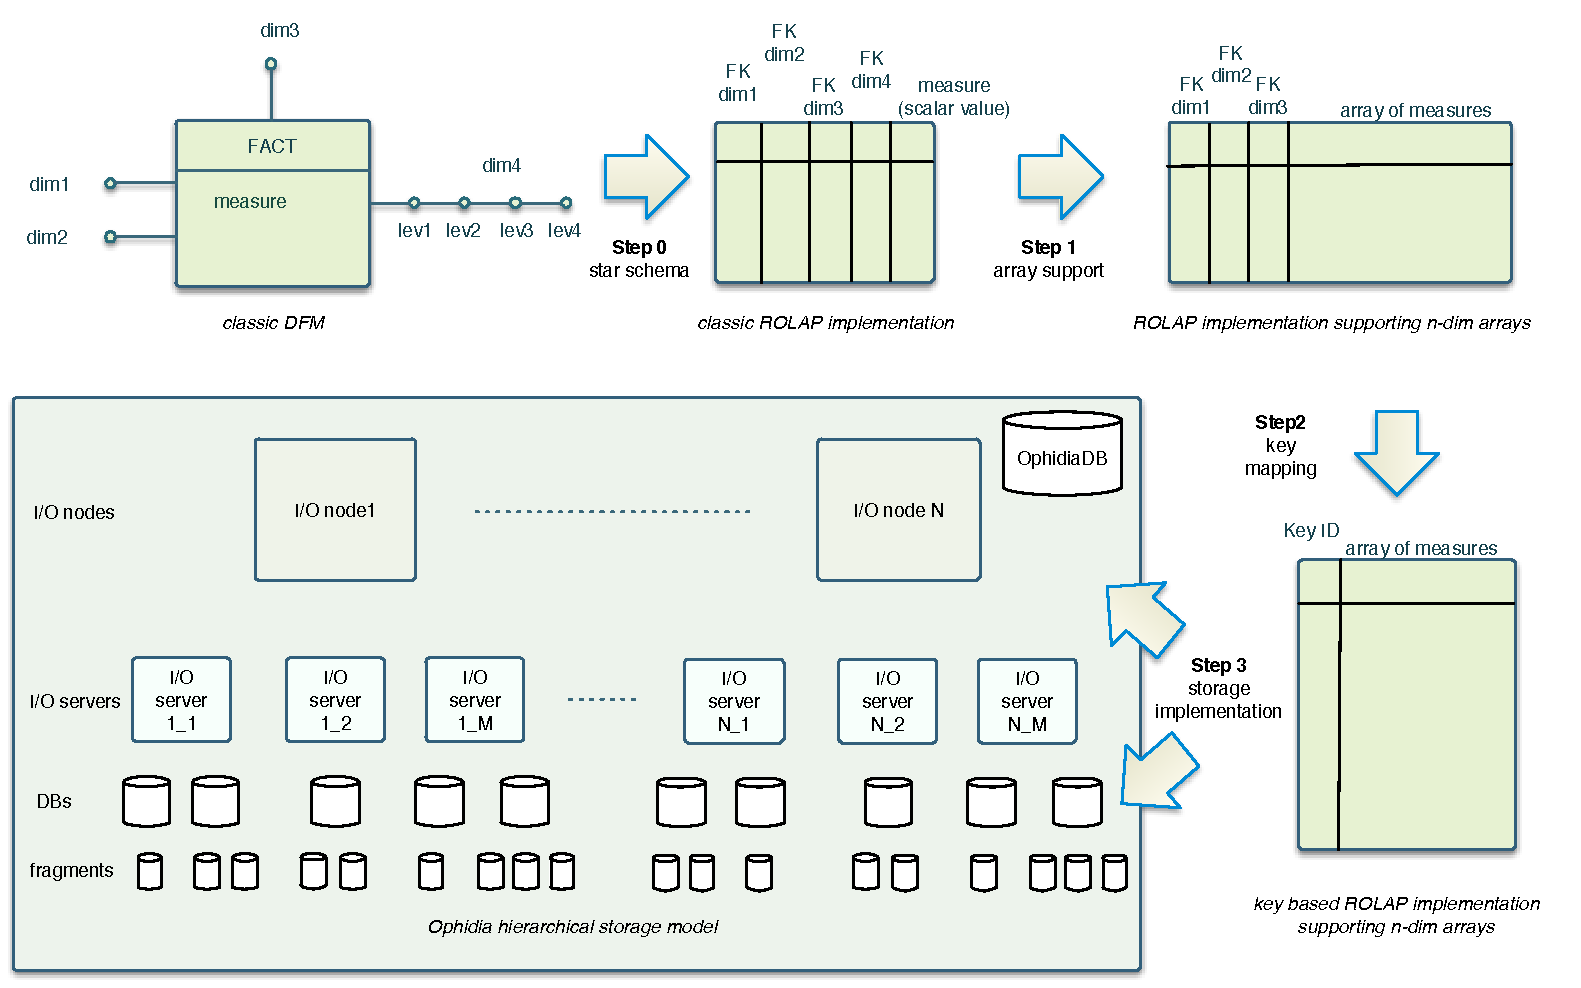
\includegraphics[width=\linewidth]{figures/Ophidia_storage_model.pdf}
	\caption{Moving from the DFM to the Ophidia hierarchical storage model}
	\label{fig: The Ophidia Storage Model}
\end{figure}

Let us consider the Dimensional Fact Model, a conceptual model for data warehouse and the classic Relational-OLAP (ROLAP) based implementation of the associated star schema. There is one fact table (FACT), four dimensions (dim1, dim2, dim3, and dim4), with the last dimension modelled through a 4-level concept hierarchy (lev1, lev2, lev3, lev4) and a single measure (measure). Let us consider a NetCDF output of a global model simulation where dim1, dim2, and dim3 correspond to latitude, longitude, and depth, respectively and dim4 is the time dimension, with the concept hierarchy year, quarter, month, day; measure represents, for instance, the air pressure.\\

\textbf{Ophidia internal storage model}\\

The Ophidia internal storage model is a two-step-based evolution of the star schema. Specifically, the first step includes the support for array-based data types while the second step includes a key mapping related to a set of foreign keys (fks). In this way, a multidimensional array can be managed using single tuple (e.g., an entire time series) and the n-tuple (fk\textunderscore dim1, fk\textunderscore dim2, ..., fk\textunderscore dimn) to be replaced by a single key (a numerical ID). It is worth noting that thanks to the second step the Ophidia storage model is independent of the number of dimensions, unlike the classic ROLAP-based implementation. Using this approach the system moves to a relational key-array schema supporting n-dimensional data management with a reduced disk space occupancy. The key attribute manages (through a single ID) a set of m dimensions (m<n), mapped onto the ID through a numerical function: \textit{ID = f(fk\textunderscore dim1, fk\textunderscore dim2, ..., fk\textunderscore dimm)}; the corresponding dimensions are called explicit dimensions. The array attribute manages the other n-m dimensions, called implicit dimensions.

In our example, latitude, longitude and depth are explicit dimensions, while time is the implicit one (in this case 1-D array) so the mapping on the Ophidia key-array data storage model consists of having a single table with two attributes:
\begin{itemize}
	\item an ID attribute: \textit{ID = f(fk\textunderscore latitudeID, fk\textunderscore longitudeID, fk\textunderscore depthID)} as a numerical datatype;
	\item an array-based attribute, managing the implicit dimension time, as a binary datatype.
\end{itemize}
In terms of implementation, several RDBMS allow data to be stored in binary form, but they do not provide a way to manage the array as a native datatype. The reason is that the available binary datatype does not look at the binary array as a vector, but rather as a single binary block: therefore, we have designed and implemented several array-based primitives to manage arrays stored through the Ophidia storage model.\\

\textbf{Hierarchical data management}\\

To manage large volumes of data, in the following, we discuss the horizontal partitioning technique that we use jointly with a hierarchical storage structure. Following the previous figure, it consists of splitting the central FACT table by ID into multiple smaller tables (each chunk is called \textit{fragment}). Many queries can execute more efficiently when using horizontal partitioning since it allows parallel query implementations and only a small fraction of the fragments may be involved in query execution (e.g., subsetting task). The fragments produced by the horizontal partitioning are mapped onto a hierarchical structure composed of four different levels:
\begin{itemize}
	\item Level 0: multiple I/O nodes (multi-host);
	\item Level 1: multiple instances of IO Server on the same I/O node (multi-IO Server);
	\item Level 2: multiple instances of databases on the same IO Server (multi-DB);
	\item Level 3: multiple fragments on the same database (multi-table).
\end{itemize}
The hierarchical data storage organisation allows data analysis and mining on a large set of distributed fragments as a whole exploiting multiple processes and parallel approaches.

\section{Big Data Concepts}

In the context of Big Data, there are many (often Java-based) technologies that address storing and processing of large quantities of data. \\

%\todo{each software solution as a paragraph?}
\textbf{Hadoop File System}\\
The Hadoop File System (HDFS) is a distributed file system that is designed to work with commodity hardware.
It provides fault tolerance via data replication and self-healing.
One limitation of its design is its consistency semantics which allows concurrent reads of multiple processes but only a single writer (WORM Model, write-once-read-many).
The data stored on HDFS are replicated in the cluster to ensure fault tolerance.
HDFS ensures data integrity and can detect loss of connectivity when a node is down.
The main concepts:

\begin{itemize}
	\item Datanode: nodes that own data;
	\item Namenode: a node that manages the file access operations.
\end{itemize}

The supported interfaces and languages are: HDFS Java API, WebHDFS REST API and libhdfs C API, as well as a Web interface and CLI shells.
Security is based on file authentication (user identity). However, HDFS accepts network protocols like Kerberos (for users) and encryption (for data).
HDFS was designed in Java for Hadoop Framework. Therefore any machine that supports Java can run it.
It can be considered as the ``source'' of many processing systems (especially in the Apache ecosystem) like Hadoop and Spark. All data stored into HDFS become ``sequence file'' files.

However, its sub-optimal performance on high-performance storage and assumption to work on cheap hardware makes it no optimal choice for HPC environments.
Therefore, many vendors support HDFS adapters on top of high-performance parallel file systems such as GPFS and Lustre.
One limitation of its design is its consistency semantics which allows concurrent reads of multiple processes but only a single writer.
\\

\textbf{HBase}\\
Apache HBase is a distributed, scalable, big data store.
HBase is an open-source, distributed, versioned, non-relational database modelled after Google's ``Bigtable: A Distributed Storage System for Structured Data'' by Chang et al. [R19]. Similarly to Bigtable, which leverages the distributed data storage provided by GFS, Apache HBase provides Bigtable-like capabilities on top of Hadoop and HDFS (https://hbase.apache.org/).
It can be used to perform random real-time read/write access to large volumes of data. HBase's goal is the hosting of large tables, on top of clusters of commodity hardware. As in the case of HDFS, this is not the optimal choice for HPC infrastructures. \\

\textbf{Hive}\\
Apache Hive is a data warehouse software facilitating reading, writing, and managing of large data sets residing in distributed storage using SQL (https://hive.apache.org/). It is built on top of Apache Hadoop and provides:
\begin{itemize}
	\item Tools to enable easy access to data via SQL, allowing data warehousing tasks such as ETL, reporting, and data analysis.
	\item Access to files stored directly in Apache HDFS or other data storage systems like Apache HBase.
The advantage is that no extract, transform or load (ETL) process is necessary. Just move the data into the file system and create a scheme on the existing files.
	\item support for query execution via various frameworks (i.e. Apache Tez, Apache Spark or MapReduce).
	\item A convenient SQL interface (including many of the later 2003 and 2011 features for analytics) to this data which allows users to explore data using SQL at a fine grain scale by accessing data stored on the file system.
\end{itemize}

\textbf{Drill}\\
Drill \footnote{\url{https://drill.apache.org}} also provides an SQL interface to existing data.

Similar to Hive, existing data can be adjusted, but in the case of Drill, data may be stored on various storage backends such as simple JSON file, on Amazon S3, or MongoDB.\\

\textbf{Alluxio}\\
Alluxio \footnote{\url{https://www.alluxio.com/docs/community/1.3/en/}} offers a scalable in-memory file system.
An interesting feature is that one can attach (mount) data from multiple (even remote) endpoints such as S3 into the hierarchical in-memory namespace.
It provides control to the in-memory data, for example, to trigger a flush of dirty data to the storage backend and an interface for pinning data in memory (similar to burst buffer functionality).
Data stored on Alluxio can be used on various big data tools.

%%%%%%%%%%%%%%%%%%%%%%%%%%%%%%%%%%%%%%%%%%%%%%%%%%%%%%%%%%%%%%%%%%%%%%%%%%%%%%%

\subsection{Ophidia Big Data Analytics Framework}
\label{sec: background/ophidia}

The Ophidia Big Data Analytics Framework falls in the big data analytics area applied to e-Science contexts.
%As introduced in \Cref{Ophidia Storage model}.
It addresses scientific use cases on large data volumes aiming at supporting the access, analysis and mining of n-dimensional array-based data. In this perspective, the Ophidia platform extends, in terms of both primitives and data types, current relational database systems enabling big data analytics tasks exploiting well-known scientific numerical libraries, a distributed and hierarchical storage model and a parallel software framework based on the Message Passing Interface to run from single operations to more complex dataflows. Further, Ophidia provides a server interface that makes the data analysis task a server-side activity in the scientific chain. Exploiting such an approach, most scientists would not need to download large volumes of data for their analysis as it happens today. On the contrary, they would download the results of their computations (typically in the megabytes or even kilobytes order) after running multiple remote data analysis operations.\\

In the following, the main features of the analytic framework of Ophidia will be depicted, the related architecture and the primitives and operators supported.\\

\textbf{The Ophidia architecture}\\

The Ophidia architecture consists of (i) the server front-end, (ii) the OphidiaDB, (iii) the compute nodes, (iv) the I/O nodes and (v) the storage system.
\begin{itemize}
	\item The server front-end is responsible for accepting and dispatching requests incoming from the clients. It is a pre-threaded server implementing standard interfaces (WS-I, OGC-WPS, GSI-VOMS). It relies on X.509 digital certificates for authentication and Access Control List (ACL) for authorisation;
	\item The OphidiaDB is the system (relational) database. By default the server front-end uses a MySQL database to store information about the system configuration and its status, available data sources, registered users, available I/O servers, and the data distribution and partitioning;
	\item The compute nodes are computational machines used by the Ophidia software to run the parallel data analysis operators;
	\item The I/O nodes are the machines devoted to the parallel I/O interface to the storage. Each I/O node hosts one or more I/O servers responsible for I/O with the underlying storage system. % described in \Cref{Ophidia Storage model}.
	\item The I/O servers are MySQL DBMSs or native in-memory services \cite{DBLP:conf/cd/EliaFDPFW16} supporting, at both the datatype and primitives levels, the management of n-dimensional array structures. This support has been adding a new set of functions (exploiting the User Defined Function approach, UDF) to manipulate arrays.
	\item The storage system is the hardware resource managing the data store, that is, the physical resources hosting the data according to the hierarchical storage structure. % defined in \Cref{Ophidia Storage model}.
\end{itemize}

\textbf{The Ophidia primitives and operators}\\

As mentioned before, the Ophidia framework addresses the analysis of n-dimensional arrays through a set of primitives included in the system as plugins (dynamic libraries). So far, about 100 primitives have been implemented. Multiple core functions of well-known numerical libraries (e.g. GSL, PETSc) have been included in new Ophidia primitives. Among others, the available array-based functions allow performing data sub-setting, data aggregation (i.e. max, min, avg), array concatenation, algebraic expressions, and predicate evaluation. It is important to note that multiple plugins can be nested to implement a single more complex array-based task.
Bit-oriented plugins have also been implemented to manage binary data cubes. Compression routines, based on zlib, xz, lzo libraries, are also available as array-based primitives.\\

Concerning the operators, The Ophidia analytics platform provides several MPI-based parallel functionalities to manipulate (as a whole) the entire set of fragments associated with a data cube. Some relevant examples include data cube sub-setting (slicing and dicing), data cube aggregation, array-based primitives at the data cube level, data cube duplication, data cube pivoting, and NetCDF file import and export.
Along with data operators, the framework provides a comprehensive set of metadata operators. Metadata represents a valuable source of information for data discovery and data description. From this point of view, some examples include provenance management, fragmentation and cube size information, variable and dimensions specific attributes.\\

\textbf{Workflows management}\\

The framework stack includes an internal workflow management system \cite{DBLP:conf/ieeehpcs/PalazzoMFDEWA15}, which coordinates and orchestrates the execution of multiple scientific data analytics and visualisation tasks (e.g. operational processing/analysis chains). It can manage the submission of complex scientific workflows using parsing and analysing input JSON files written in compliance with a predefined JSON Schema, which includes the description of each task, the definition of the dependencies among different tasks, and several metadata. In addition, advanced features as the definition of loops, variable definition and conditional statements are available. Workflow execution monitoring is allowed by explicitly querying the Ophidia server or in real-time through a graphical user interface.

\subsection{MongoDB}
The MongoDB\footnote{\url{https://docs.mongodb.com/}} is an open-source document database.
Its architecture is high-performant and horizontally scalable for cluster systems.
MongoDB offers a rich set of interfaces, e.g., RESTful access, C, Python, Java.

The data model of MongoDB provides three levels:
\begin{itemize}
  \item database: follows our typical notion; permissions are defined on the database level.
  \item Document: This is a BSON object (binary JSON) -- consisting of subdocuments with data.
  An example of JSON is shown in \Cref{lst:mongoJSON}.
  Each document has the primary key field: \_id. Either the field must be manually set, or it will be automatically filled.

  \item Collection: this is like a table of documents in a database. Documents can have individual schemas. It supports indices on fields (and compound fields).
\end{itemize}
To access data, one has to know the name of a database (potentially secured with a username and password), collection name. All documents within the collection can be searched or manipulated with one operation.

In the example of \Cref{lst:mongoJSON}, it would also be possible to create one document for each person and use the $\_id$ field with a self-defined unique ID such as a tax number.

\begin{tcbcode}[label={lst:mongoJSON}]{Example MongoDB JSON document}
\begin{lstlisting}
"_id" : ObjectId("43459bc2341bc14b1b41b124"),
"people" : [ # subdocuments:
    { "name" : "Max", "id" : 4711, "birth" : ISODate("2000-10-01")},
    { "name" : "Lena", "id" : 4712, "birth", ... }
  ]
\end{lstlisting}
\end{tcbcode}


MongoDB's architecture uses sharding of document keys to partition data across different servers.
Servers can be grouped into replica sets to provide high availability and fault tolerance.

\paragraph{Query documents}

A query document is a BSON document that is used to search all documents of a collection for data that matches the defined query.
The example in \Cref{lst:mongoQuery} specifies documents that contain the sub-documents people with an id field that is bigger than 4711.
Complex queries can be defined.
In combination with indices on fields, MongoDB can search large quantities of documents quickly.

\begin{tcbcode}[label={lst:mongoQuery}]{Example MongoDB Query document}
\begin{lstlisting}
{ "people.id" : { $gt : 4711 } }
\end{lstlisting}
\end{tcbcode}





%%%%%%%%%%%%%%%%%%%%%%%%%%%%%%%%%%%%%%%%%%%%%%%%%%%%%%%%%%%%%%%%%%%%%%%%%%%%%%%
\chapter{Requirements}
\label{sec:requirements}
\begin{chapterIntro}
The goal of this section is to provide high-level requirements: what the system needs to do and how it relates to dependencies. The chapter distinguishes between functional and non-functional requirements.
Functional requirements that are the required features to fulfil the application of the system are enumerated in \Cref{sec: requirements/functional}.
Non-functional requirements that relate to the run time qualities (e.g., performance, fault-tolerance or security) of the architecture are collected in \Cref{sec: requirements/non functional}.
\end{chapterIntro}

\label{chap:requirements}


\section{Functional Requirements}
\label{sec: requirements/functional}

The developed system is a storage system, thus provides basic means to access and manipulate data
and, thus, provides an API suitable for use in current and next-generation high-performance simulation environments:

\begin{enumerate}
\item CRUD-operations -- Create, Retrieve, Update (append), Delete data in scientific relevant granularity.
\begin{itemize}
\item Partial access --
It must be possible to either retrieve (access) the complete results from experiments or to identify sections of interest and access those.
\end{itemize}
\item Discover, browse and list data. It must be possible to identify the file or object which contains interesting data, and eventually obtaining an identifier for the object and an endpoint through which it can be accessed.

\item Handling of scientific/structural metadata as the first-class citizen that means the storage system understands the metadata, and the API is designed to exploit this knowledge, e.g., data can be searched by consulting metadata catalogues.
\item Semantical namespace, meaning that objects can be searched and accessed based on the structural metadata and not by a single hierarchical namespace.
\item Supporting heterogeneous storage -- the system shall exploit a heterogeneity of hardware technology, that means using the individual storage technologies for the best purpose, i.e., the characteristics of the storage define their use within ESD. At best, the system makes these decisions without user intervention, but it may require users to provide certain ``hints'' or intents how data is and will be used, which includes cases such as:
\begin{enumerate}
    \item Caching data on faster storage tiers
    \item Explicit migration, where for example, users explicitly tag their data for a ``lower'' tier of storage (cheap and/or slow), but the ESD system needs to cache the data en-route to tape.
    \item Overflow, where for example a particular deployed ESD system is unable to handle new data stores to disk without flushing old data to tape.
    \item Transparent (and/or non-transparent) data migration, e.g., data migrate from tape to disk in response to full or partial read requests through one of the ESD interfaces.
\end {enumerate}


%Currently most weather and climate centres deploy an HPSS system of some sort in their environment, which is usually very costly. The ESD storage system will need to have at least some kind of internal hierarchy and caching system.

\item Function shipping -- support the transfer of compute kernels to the storage system and process data somewhere in the I/O path. This feature reduces data movement which is costly on Exascale systems.

\item Compatibility -- for backwards compatibility with existing climate and NWP applications, the system must expose or support existing APIs, e.g.,
\begin{itemize}
\item a NetCDF interface
\item an HDF5 interface %suitable to be bound into client HDF libraries deployed both locally (LAN) and remotely (WAN),
\item a GridFTP interface
\item a POSIX file system interface
\item a suitable RESTful interface
\end{itemize}
In particular, it shall be possible to create data using one interface and accessing the data without conversion using another.
\end{enumerate}



Supporting requirements accompany these mandatory requirements:
\begin{enumerate}
\item Auditability -- upon request, object-specific operations need to be logged, in particular, all creations, retrievals, and updates discriminated by users.
\item Configurability -- A system-wide configuration of all available storage resources and their performance characteristics must be possible.
\item Notifications -- A tool or user may subscribe for an object and be notified if certain modifications are made to the object. This feature allows the watching of the changelog of objects efficiently without polling.
\item Import/Export -- tools to support data exchange in or out of the ESD system.
Depending on the format, conventions for mapping the format internal metadata or supplying metadata needed to meet internal ESD metadata requirements.
\item Access control -- it should be able to restrict access to objects, supporting several roles, e.g., data centre staff, users, projects.
\begin{itemize}
\item Data sharing -- In particular, the system should make it simple to share data with other researchers.
\end{itemize}
\end{enumerate}



\section{Non-Functional Requirements}
\label{sec: requirements/non functional}


For productive use in a data centre, these requirements are mandatory:
\begin{enumerate}
\item Performant --- coping with volume/velocity and delivering adequate bandwidth and latency. The system is efficient and exploits available performance from hardware (network and storage technology), at best 90\%+ of the available raw network bandwidth and storage system throughput is achievable from applications.
\item Reliable --- stored data is durable. In transit data corruption and silent data, corruption is detected and corrected. In case an uncorrectable error occurs, the data that is affected can be identified, and the still correct parts of affected objects shall still be accessible. Reliability includes:
  \begin{itemize}
  \item Fault Tolerant --- able to detect and repair hardware and software failures.
  \item Highly-available --- data access shall be possible even with partially broken hardware and software, thus, meeting expectations of users similar to that they have of conventional disk sub-systems.
  \end{itemize}
\item Versatile ---  able to utilise existing heterogeneous storage infrastructures, including, but not limited to
  \begin{itemize}
  \item existing traditional storage systems such as tape, object store, and parallel file system,
  \item existing non-traditional storage systems such as the HDFS, and
  \item potential new storage systems such as burst buffers or NVRAM.
  \end{itemize}
\item User-friendly -- the system shall provide good usability, this includes:
  \begin{itemize}
  \item Transparency --- hides specifics of the storage landscape and does not \textit{\textbf{require}} users to set and define technical parameters specifically to a given system.
  \item Portability --- code that uses the developed APIs should work in different data centres, i.e., with different hardware and software.
  \end{itemize}
\item Cost-Effective --- the software system should be affordable and maintainable by data centre staff at Exascale.

\item Standards-based --- using interfaces, formats and standards which maximise re-usability.
\end{enumerate}


%\section{Related Work and Dependencies}
%In this section we discuss the influence of important third-party architectures on the ESD requirements.
%\label{sec:related}
% In which we discuss relationships to key projects such as JR's HDF server activity, Ophidia etc.
%\subsection{The Highly Scalable Data Storage Project}

% Intro paragraph describing the project aims
The HDF group in \dots
\todo{Update the description of the HSDS project}

We here repeat some of the requirements and assumptions from that project,
recognising that because we desire that the ESD is as compatible with the HSDS system as possible, most of these assumptions and requirements apply to the ESD
system as well.

\paragraph{Key Object Storage Assumptions}. The HSDS project makes the following assumptions about objects and the interactions with the object storage system:
\begin{enumerate}
    \item Files and Objects: Files are shared into objects.
    \item Key size: Object keys are limited to 1024 characters.
    \item Key names: The first 3-4 characters of the keys should be randomly distributed (to avoid request rate limits due to a single storage system be targeted for systems such as AWS where key names influence object location).
    \item Object size needs to follow the ``goldilocks principle'' needing to be not too small, and not too large: dealing with too many small objects would be prohibitively expensive in a public cloud and the use of very large objects ($>$ 100 MB) would introduce excessive latency.
    \item Updates to a storage object will be complete (i.e. the entire object will be overwritten), atomic (i.e. last writer wins), and either succeed or fail --- and in the latter case there should be no update to the object.
    \item Partial reads could be possible, though.
    \item The object storage system will not provide support for ``transactions'' (i.e. the ``all or nothing'' update of two or more objects).
    \item The storage system will not be read-write consistent.
    \item Metadata associated with each object will be at least 1024 bytes long.
    \item All objects managed by any service instance will exist in one ``bucket'' for which that service will need read-write authority.
\end{enumerate}

With these assumptions, we might expect that the HSDS (and hence ESD services) would need to perform a number of data management functions that are not provided by the underlying object storage paradigm:
\begin{enumerate} [resume]
    \item Listing of files, and file permissions, will need to be managed by a service (listing keys will generally be inefficient (and would not work well with randomly distributed keys), and file permissions are notions that belong in HSDS/ESD metadata space, not in the storage system).
    \item The reverse lookup between an object and the parent file will need to be explicilty managed by a service (an object will not itself know of its parent).
    \item All object creation and update needs to be managed through a service interface. Object retrieval may be either via a service which aggregates objects on the server side, or via a client which aggregates objects after interrogating a service to find appropriate objects.
\end{enumerate}
These functions are naturally provided by traditional (POSIX) file systems.




%%%%%%%%%%%%%%%%%%%%%%%%%%%%%%%%%%%%%%%%%%%%%
\chapter{Use-Cases}
\label{chap:use cases}

\begin{chapterIntro}
This chapter discusses some use-cases for a middleware to handle earth system data.
\Cref{sec:use cases/climate and weather} starts with a high level perspective to common workloads in climate and weather forecasts.
It follows an introduction of involved stakeholders/actors (see \Cref{sec:use cases/actors}) and systems (see \Cref{sec:use cases/systems}).
\Cref{sec:use cases/use cases} and following are the actual use cases.
Use cases can extend each other, and are generally constructed in a way that they are not limited to the ESDM but also apply to similar middleware.
In addition, the use of backends is kept abstract where possible, so that in principle implementations can be swapped with only minor semantic changes to the sequence of events.
\end{chapterIntro}



%%%%%%%%%%%%%%%%%%%%%%%%%%%%%%%%%%%%%%%%%%%%%%%
\section{Climate and Weather Workloads}
\label{sec:use cases/climate and weather}

The climate and weather forecast communities have their characteristic workflows and objectives, but also share a variety of methods and tools (e.g., the ICON model is used and developed together by climate and weather scientists).
This section briefly collects and groups the data-related high-level use-cases by community and the motivation for them.

Numerical weather prediction focuses on the production of a short-time forecast based on initial sensor (satellite) data and generates derived data products for certain end users (e.g., weather forecast for the general public or military).
As compute capabilities and requirements for users increase, new services are added or existing services are adapted.
Climate predictions run for long time periods and may involve complex workflows to compute derived information such as monthly mean or to identify certain patterns in the forecast data such as tsunamis.
%before the community settles for large scale ensemble simulations the models go two a continues process of model and performance optimizations.

In the following, a list of characteristic high-level workloads and use-cases that are typically performed per community is given.
These use-cases resemble what a user/scientist usually has in mind when dealing with numerical weather prediction (NWP) and climate simulation; there are several supportive use-cases from the perspective of the data centre that will be discussed later.


\paragraph{Numerical Weather Prediction}

\begin{itemize}
	\item Data ingestion: Store incoming stream of observations from satellites, radar, weather stations and ships.
	\item Pre-Processing: Cleans, adjusts observation data and then transforms it to the data format used as initial condition for the prediction. For example, insufficient sampling makes pre-processing necessary so models can be initialized correctly.
	\item Now Casting (0-6h): Precise prediction of the weather in the near future.
	Uses satellite data and data from weather stations, extrapolates radar echos.
	\item Numeric Model Forecasts (0-10+ Days): Run a numerical model to predict the weather for the next few days.
	Typically, multiple models (ensembles) are run with some perturbed input data.
	The model proceeds usually as follows: 1) Read-Phase to initialize simulation; 2) create a periodic snapshots (write) for the model time, e.g., every hour.
	\item  Post Processing: create data products that may be used for multiple purposes.
	\begin{itemize}
		\item for Now Casting: multi sensor integration, classification, ensembles, impact models
		\item for Numeric Model Forecasts: statistical interpretation of ensembles, model-combination
		\item generation of data products like GRIB files as service for customers of weather forecast data
	\end{itemize}
	\item Visualizations: Create fancy presentations of the future weather; this is usually part of the post processing.
\end{itemize}


\paragraph{Climate}

Many use cases in climate are very similar:

\begin{itemize}
	\item Pre-Processing: Similar to the NWP use case.
	\item Forecasting with Climate Models: Similar to the NWP use case, with the following differences:
	\begin{itemize}
		\item The periodic snapshots (write) uses variable depending frequencies, e.g., some variables are written out with higher frequencies than others
	\end{itemize}
	\item Post Processing: create data products that are useful, e.g., run CDOs (Climate Data Operations) to generate averages for certain regions. The performed post processing depends on the task the scientist has in mind. While at runtime of the model some products are clear and may be used to diagnose the simulation run itself, later scientists might be interested to run additional post processing to look for new phenomena.
	\item Dynamic visualisation: use interactive tools to search for interesting patterns. Tools such as VTK and  Paraview are used. %Potentially create a time series movie.
	\item Archive data: The model results are stored on a long-term archive. They may be used for later analysis --  often at other sites and by another user, e.g., to search for some interesting pattern, or to serve as input data for localized higher-resolution models. Also it supports reproduceability of research.
\end{itemize}

Note that compared to NWP there is more dynamic and flexibility needed in climate forecasting.
Scientists may run prototypical code simulating novel features and creating new data products.
They may use many different tools on different sites to post process and visualize data and, over time, new methods may be found to interact with data model output.

%%%%%%%%%%%%%%%%%%%%%%%%%%%%%%%%%%%%%%%%%%%%%%%
\section{Roles and Human Actors}
\label{sec:use cases/actors}

This section introduces the involved actors and provides an overview to the use cases addressed in this chapter.
Research is often funded in relatively short term projects with a set of defined improvements to the state of the art.
Projects are often embedded with already existing institutions such as universities or research laboratories.
\Cref{fig:esiwace_usecases} visualises the project perspective to data creation and analysis.
An experimenter usually prepares and runs a model, the preparation may include ingestion of data (migration of data into ESD) and pre-processing this data.
An analyst analyses model output and generates useful data products.
In this process, he/she may retrieve a selected subset of data to a local machine to foster rapid data exploration.
These use cases shall be supported on an exascale demonstrator.
In general, we refer to scientists as users of ESDM.



\begin{figure}
	\centering
	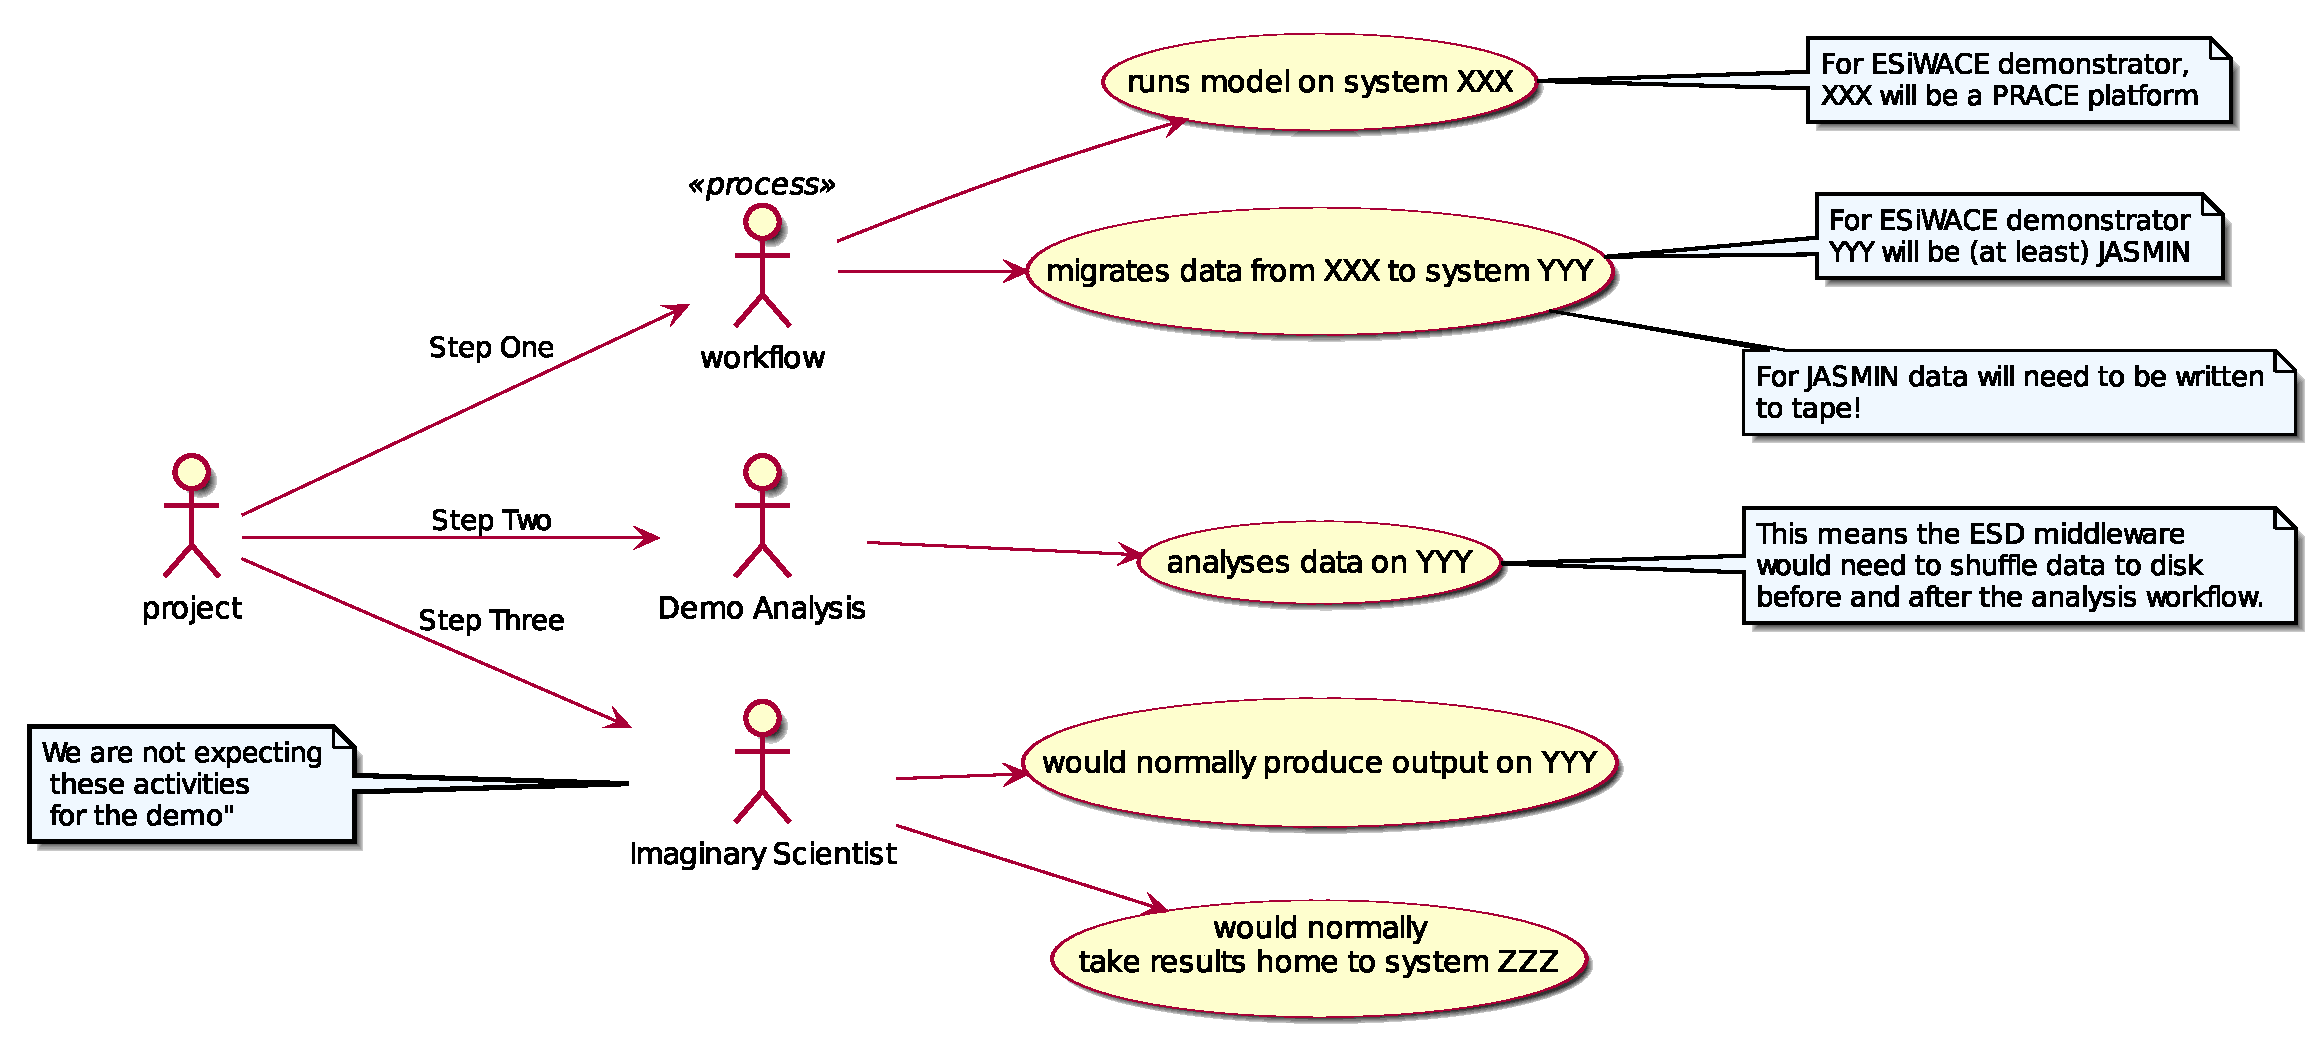
\includegraphics[width=0.75\linewidth]{use-cases/uml/generic/esiwace_usecases.eps}
	\caption{Different roles and tasks commonly seen within an earth system related project.}
	\label{fig:esiwace_usecases}
\end{figure}



\medskip

Commonly, scientists share technical infrastructure such as compute and storage systems with other groups within an organisation.
But as scientists collaborate across the boundaries of their institution, the operation of, e.g., a data center is outsourced and embedded into a separate organisation (such as the DKRZ, ECMWF or Met office) with the different organisations as stakeholders.
Yet, it is not uncommon to find smaller systems operated by individual research groups for analysis tasks.
%\Cref{fig:use_case_relationships} illustrates the various actors that are involved in data management within and across sites.
A role in this context does not translate to persons, but a person may fill multiple roles, but also multiple persons may collaborate on a single role.



%\begin{figure}
%	\centering
%	\includegraphics[width=0.5\linewidth]{use-cases/uml/generic/data-center-roles.eps}
%	\caption{User and data management actors in a scientific computing environment. In many cases multiple roles maybe fulfilled by the same person.}
%	\label{fig:use_case_relationships}
%\end{figure}

\medskip

The use cases described in this chapter, are illustrated in \Cref{fig:overview-actors-use-cases}.
In general, by use case we mean a typical workflow that may consist of multiple steps that are run sequentially or in parallel (concurrently).
It covers the execution of applications (Simulation),
the pre/post processing of data needed to drive applications,
the concurrent simulation and post processing, i.e., while the simulation runs we already produce relevant data products,
the simulation coupled with in-situ post processing,
the simulation coupled with interactive visualisation,
the simulation coupled with tools for big data analytics.
These use cases are built on the generic use cases for independent write and read.


An experimenter (user) has a use case in mind that consists of multiple steps (jobs) that are run sequentially or concurrently.
He/she submits a job of the workflow to the job scheduler which assigns resources on the supercomputer and starts the execution of the job script.
Optionally, it may use the ESDM interfaces to steer data migration and staging or additional optimizations.
The job script runs on one of the allocated nodes and processes a sequence of instructions such as running of applications.
An application may use the ESDM interface directly or via an existing API such as NetCDF indirectly.




\begin{figure}
	\centering
	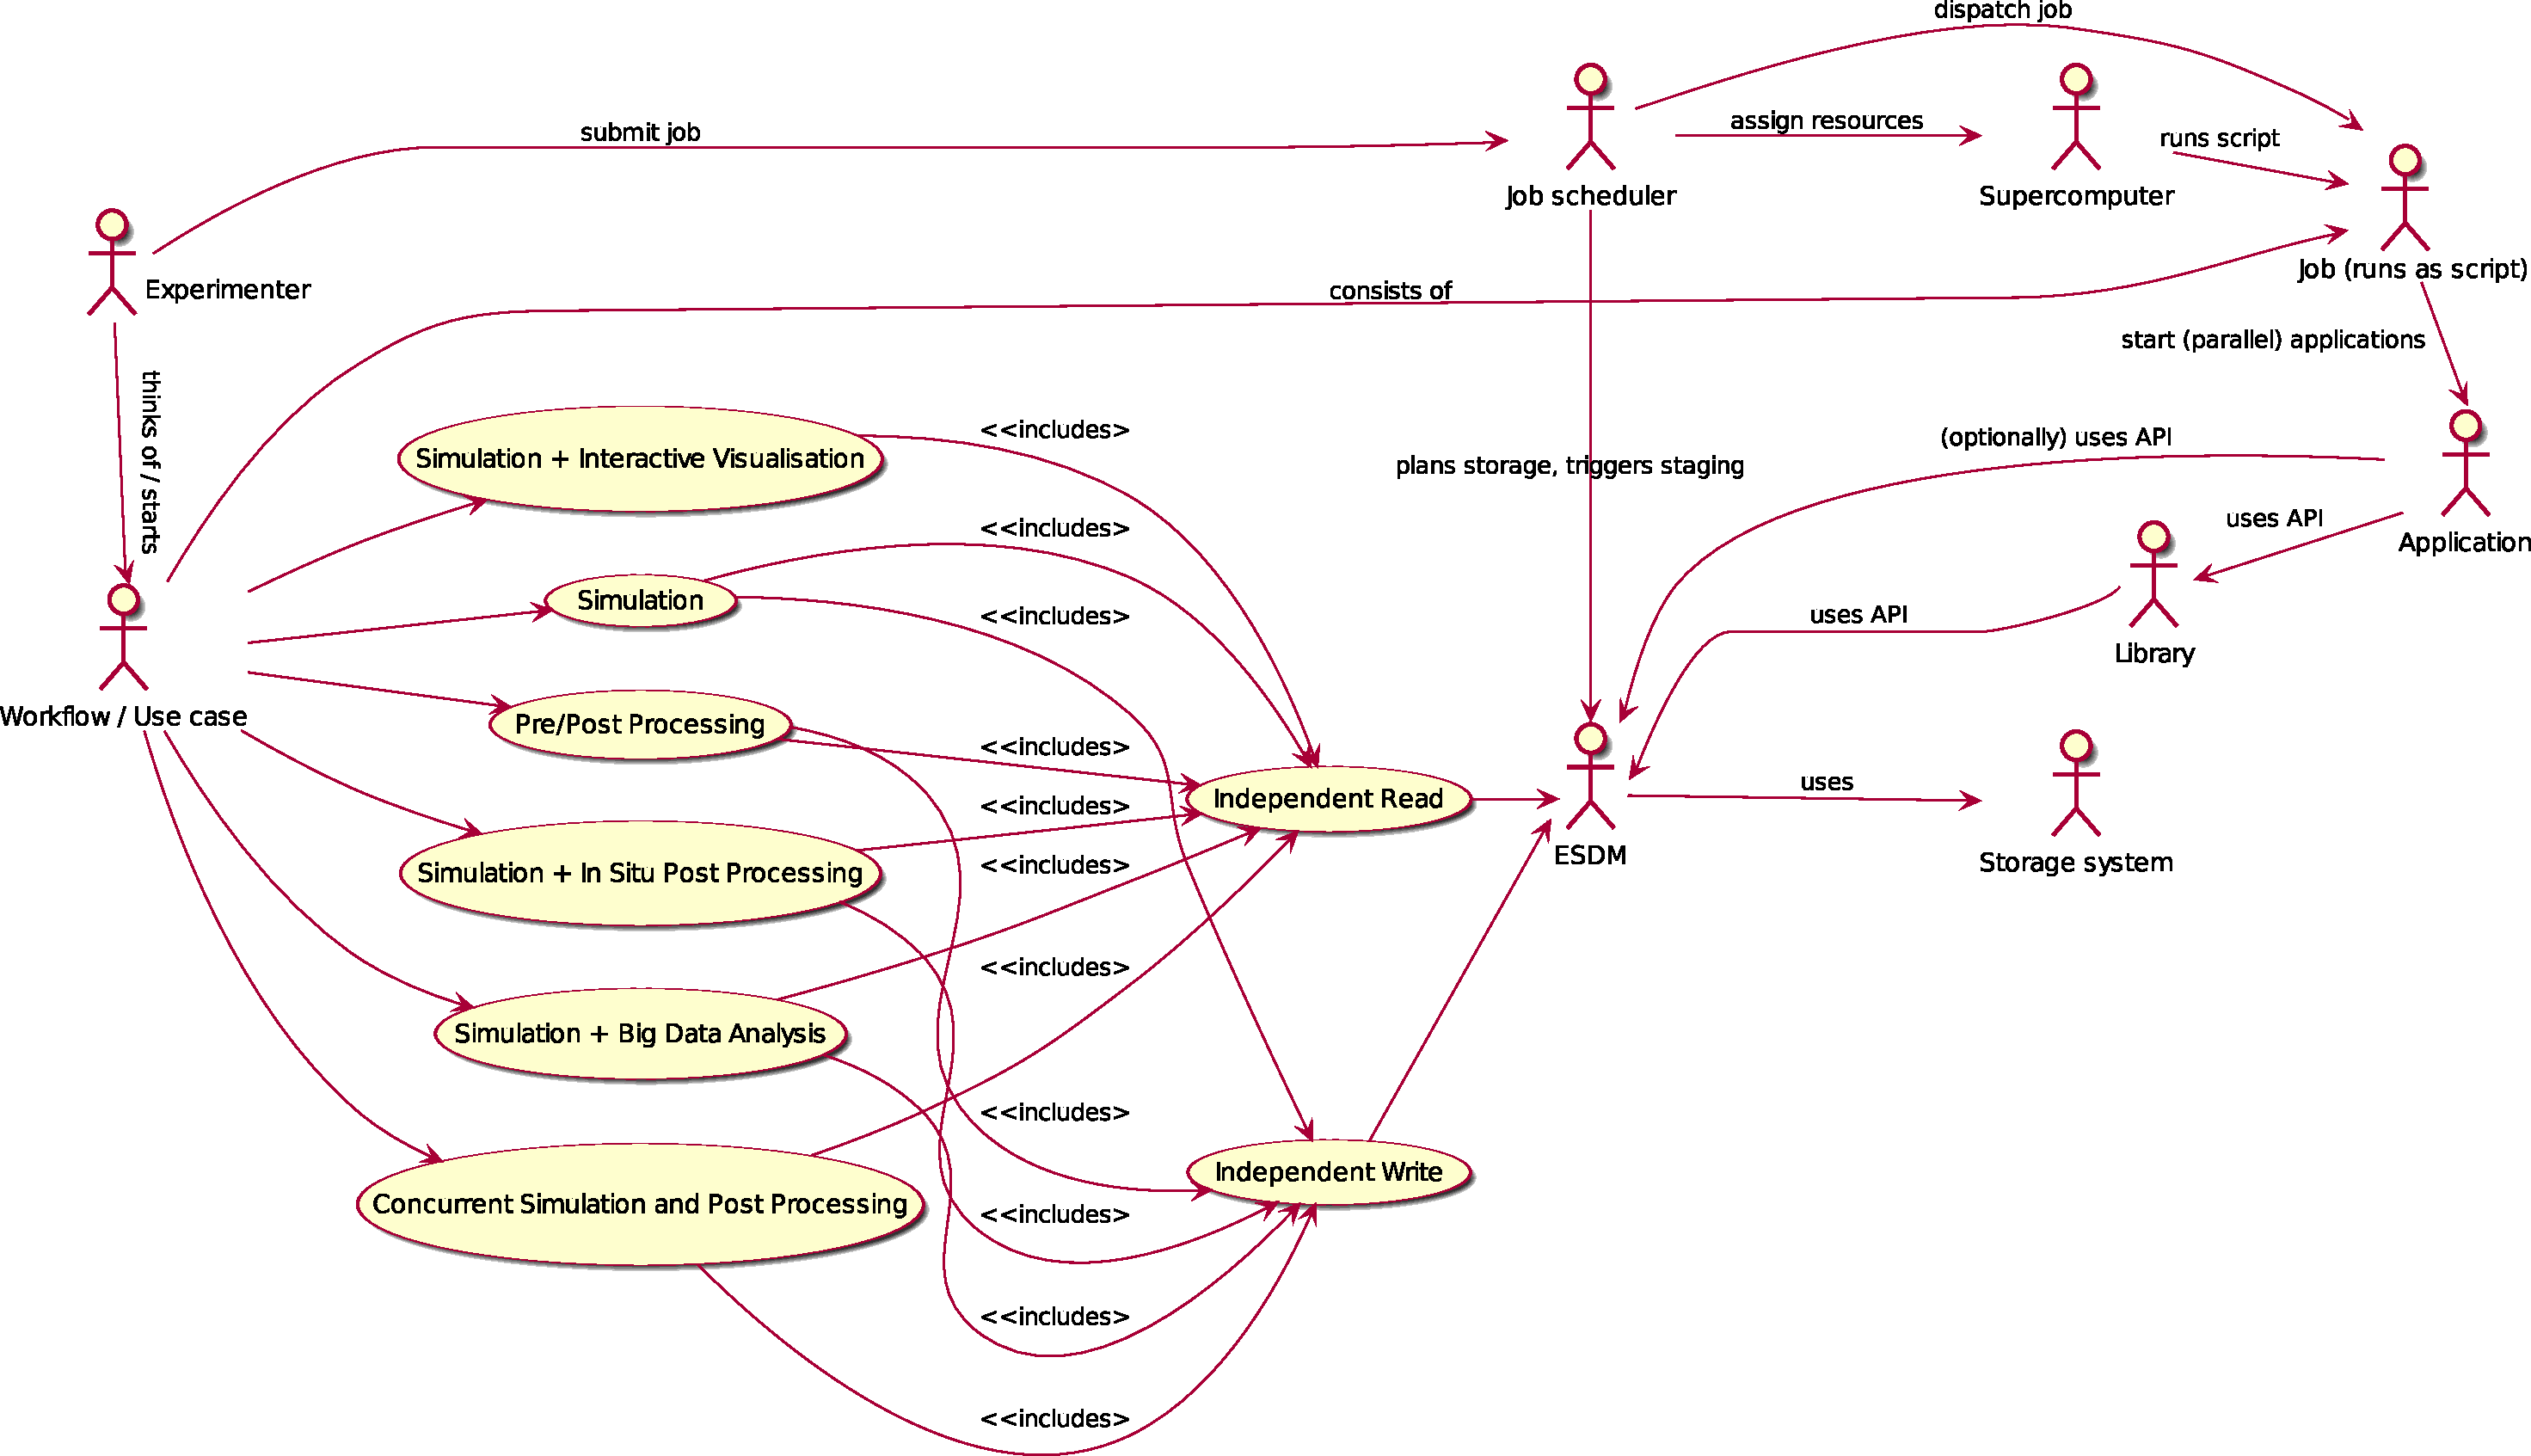
\includegraphics[width=\linewidth]{use-cases/uml/generic/use-case-overview-manual}
	\caption{Overview of described actors and use cases.}
	\label{fig:overview-actors-use-cases}
\end{figure}





\subsection{Credentials and Permissions of Actors for Data Access}

The introduction captured the logical view for the different actors managing and using data.
A more technical perspective can be described as follows.
There are three general types of actors who can interact with an earth system storage resource:

\begin{itemize}
	\item Unprivileged Users (e.g, external partners, that only download or read available data)
	\item Privileged Users (Project participants, with varying privileges)
	\item Administrators (Site/Infrastructure operators)
\end{itemize}

In the following, we use the term object to refer primarily to something with equivalent semantics to a file.
A more fine-grained object access will also be available via any APIs exposed by the service.

\subsection*{Unprivileged User}

An unprivileged user is someone who has only read-only access. These users can:
\begin{itemize}
	\item navigate content, using faceted browse against public tags,
	\item list all (public) tags to which they have access,
	\item given a tag, list all tags carried by objects with the first tag,
	\item given a list of tags, list all tags carried by objects with all members of that list,
	\item given a tag list, list all objects with the union set of all those tags,
	\item retrieve any visible object from the list of objects presented by any tag list,
	\item interact with any visible object via limited read only operations.
\end{itemize}

\subsection*{Privileged Users}

A privileged user is someone who has CRUD access to (their) content within the archive as well as all the abilities of an unprivileged user applied to their own content. They can:
\begin{itemize}
	\item create, retrieve, update, and delete content within prescribed quotas,
	\item control access to their objects (see below),
	\item assign tags to objects,
	\item navigate both public or (own) private tags.
\end{itemize}

Controlling access:
\begin{itemize}
	\item Users can create ``group'' identifiers, and associate user identifiers with that group.
	\item They must themselves be members of any group they create.
	\item They can add/remove any other user identifiers known to them to that group.
	\item How users find the identifiers of other users is not defined here.
	\item If they use the identifier ``public'' for a group, then users in this group (who may also include the special identifier "anonymous"), then users in this group will have read-only access to these objects.
	\item Users can assign any group identifier of which they are a member to any object they create. In doing so, they make ``their'' objects into ``shared'' objects (except for the public group as defined above, where they are simply making the object read-only to that group).
	\item Any user with ``shared'' access has the same privileges for that object as the original owner, except that of modifying or removing the group tag.
	\begin{itemize}
		\item This means they can delete, update, and retrieve the object. Of course deleting it will disassociate the group tag.
	\end{itemize}
	\item Users can list the groups of which they are members, and list the members of any of those groups.
\end{itemize}

Note that this usage of group is not identical to the concept of UNIX groups, because users control their definition.

\subsection*{Administrators}

Administrators can:

\begin{itemize}
	\item  start and stop any service,
	\item  access all data held by all privileged users,
	\item  manage privileged users: create, update, delete users,
	\item  allocate quotas, i.e., define available storage space for users and groups,
	\item  retrieve usage information,
	\item  configure the layout of content in the service against available storage resources,
	\item  migrate content within the storage resources (a process that might temporarily disable user access while the migration takes place)
	\item  configure any required compute, cache, and network services.
\end{itemize}


%%%%%%%%%%%%%%%%%%%%%%%%%%%%%%%%%%%%%%%%%%%%%%%
\clearpage
\section{Systems}
\label{sec:use cases/systems}


This section describes the most important hardware and storage components that are used by the use cases.
Each system has a description, and if applicable a list of related subsystems.
In addition, for every subsystem risk factors and failure modes of the system are collected, which then can be easily addressed by the individual use cases.

Each system comes with a short description, an illustration briefly explaining the architecture, a list of associated risks as well as a list of associated subsystems.
It follows a more detailed description of each section:

\paragraph{System Description:} A brief description of the system, common practices and relations to other systems.
\paragraph{Risks:} Typical risks and failure modes associated with the system.
\paragraph{Subsystems:} If the system is split into subsystems, this includes a list with references to each subsystem.

%%%%%%%%%%%%%%%%%%%%%%%%%%%%%%%%%%%%%%%%%%%%%%%%%%%%
\subsection{System: Supercomputer}
\label{System: Supercomputer}

\begin{figure}
	\centering
	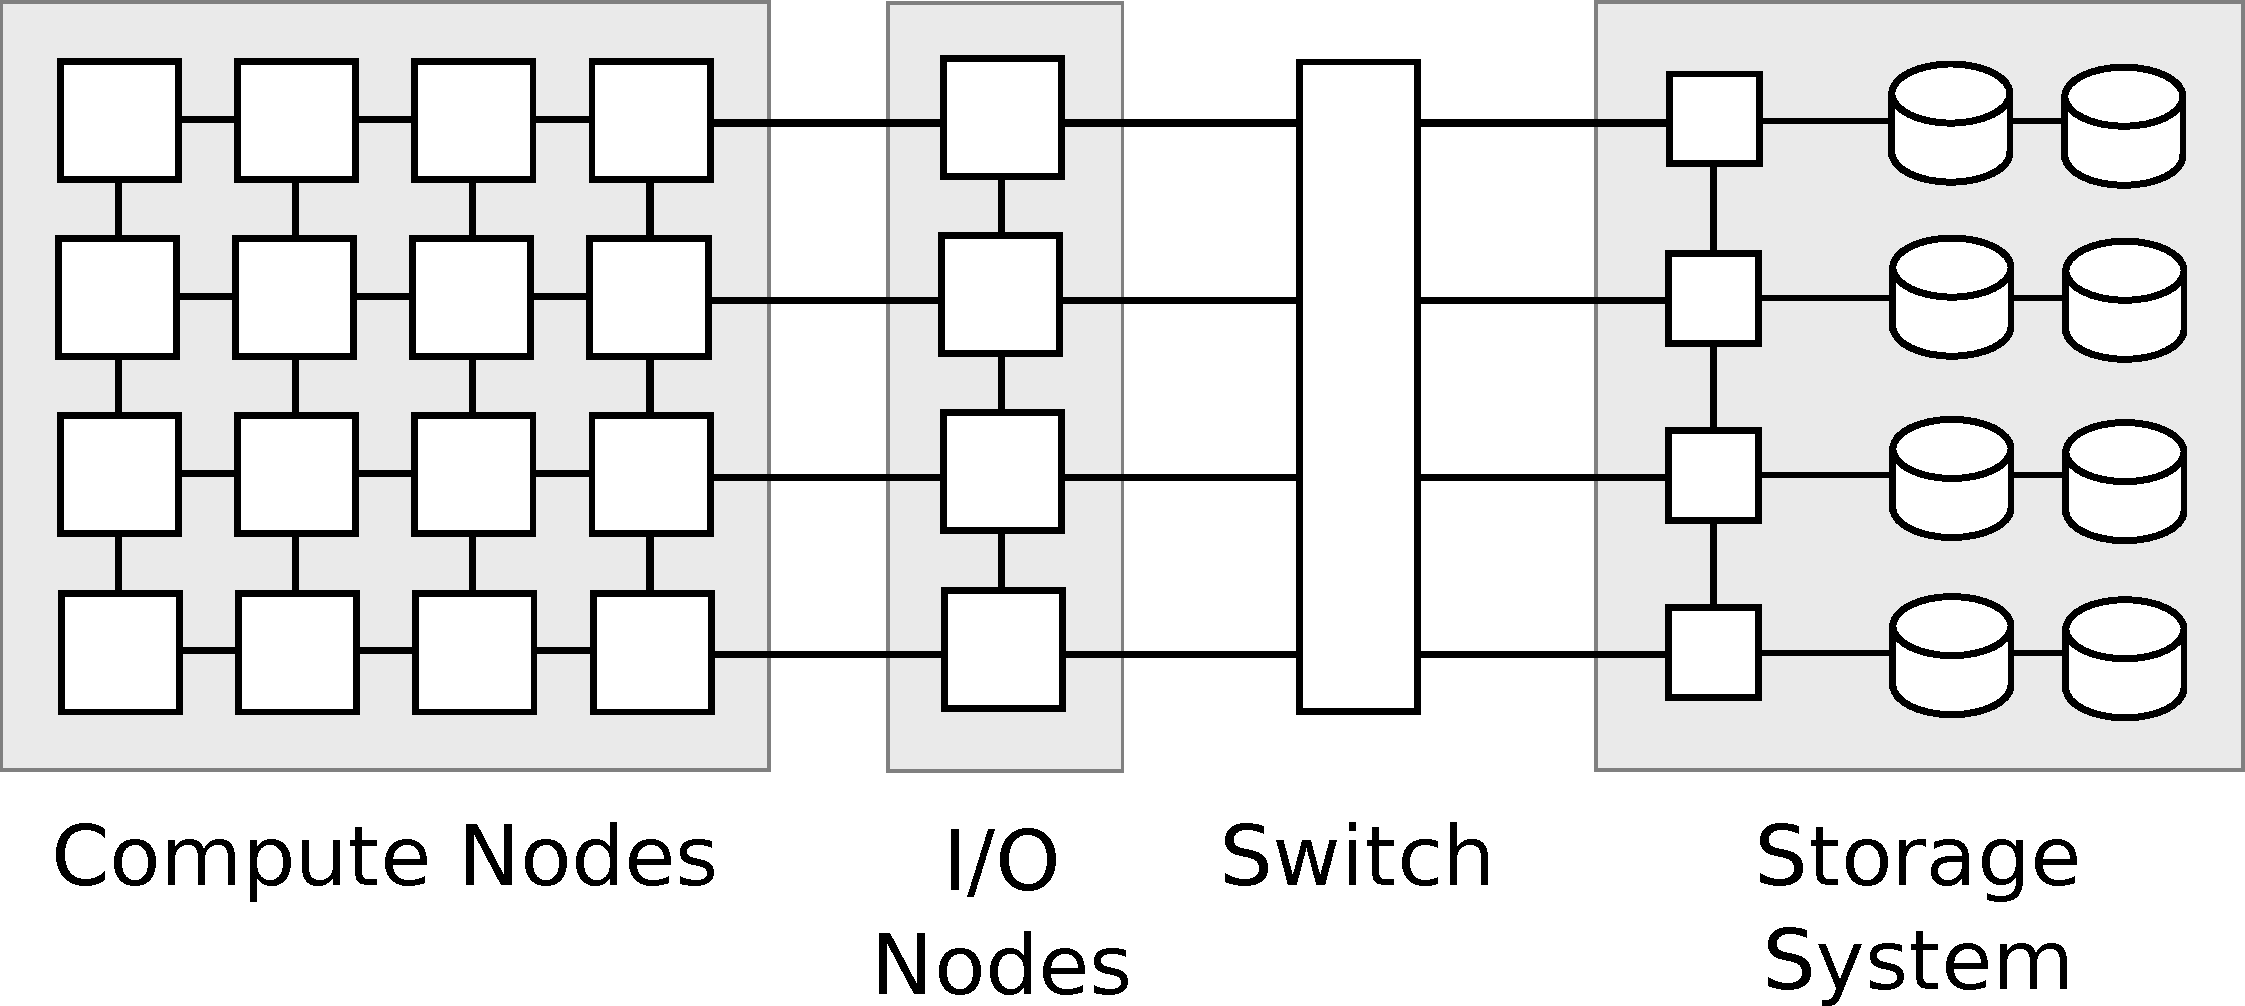
\includegraphics[width=0.5\linewidth]{use-cases/systems/hpc_clean}
	\caption{A typical supercomputer with compute notes connected via a high performing network interconnect and a dedicated storage system.}
	\label{fig:system supercomputer}
\end{figure}


\paragraph{System Description:}
An HPC system here is assumed to be a cluster computer with 100 to 100.000 cores/nodes.
The nodes are connected via a network, often a specialised high-throughput, low-latency interconnect (e.g., Infiniband). An HPC system usually does not stand by itself but is also connected to a high-performance storage system.
\Cref{fig:system supercomputer} illustrates a commonly seen deployment of a supercomputer, though many details are ignored as the exact topology depends on the specific applications and systems deployed.
Resource allocations are commonly managed using a job scheduler that allows users submit jobs.


\paragraph{Risks:}
\begin{itemize}
	\item Hardware failures (a growing concern in expectation of exascale)
	\item Data loss and corruption (silent)
\end{itemize}


\paragraph{Subsystems:}


\begin{itemize}
	\item Compute Nodes: The raw compute resources. CPUs + Memory
	\item Storage System: A network attached storage system. Disk/SSD based, and maybe long-term (e.g., Tape) (see \Cref{System: Storage System})
	\item Applications (see \Cref{System: Application})
	\item Job Scheduler: Applications/Tasks are submitted to a batch system that manages resource allocations. (see \Cref{System: Job Scheduler})
\end{itemize}



%%%%%%%%%%%%%%%%%%%%%%%%%%%%%%%%%%%%%%%%%%%%%%%%%%%%
\subsection{System: Storage System}
\label{System: Storage System}

\begin{figure}
	\centering
	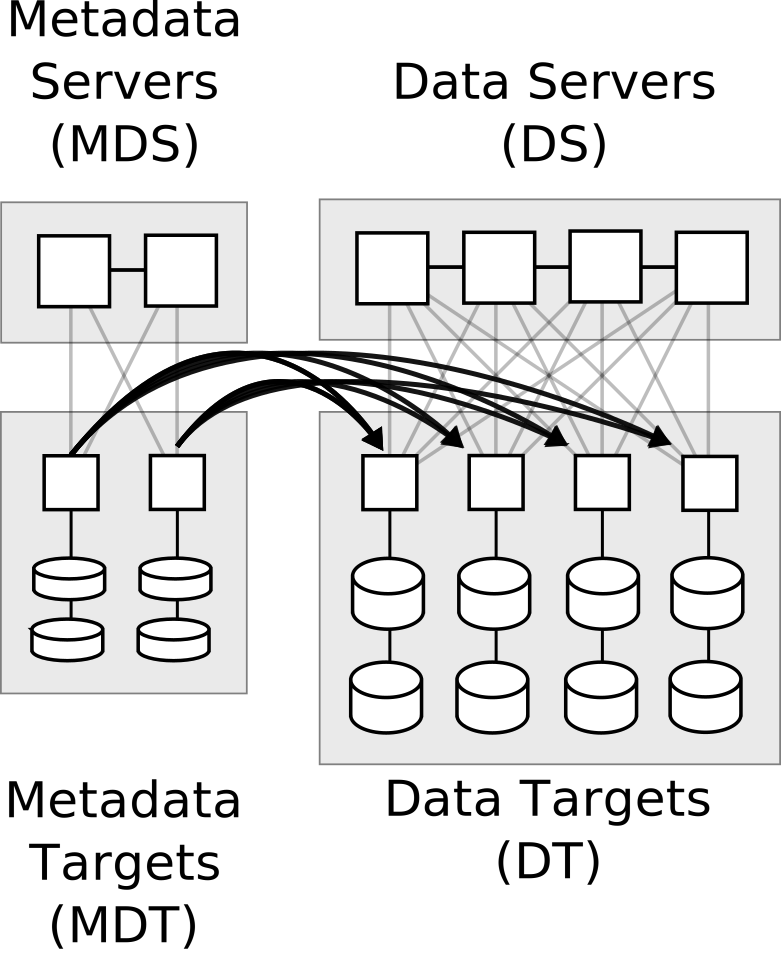
\includegraphics[width=0.33\linewidth]{use-cases/systems/storage_clean}
	\caption{A more nuanced variant of a common deployment model for storage systems. Data and metadata are handled by differently configured hardware. }
	\label{fig:System: Storage System}
\end{figure}


\paragraph{System Description:}
A system to provide (high performance) access to stored data.
Usually a large disk-based system, that exposes either a file system or and object store to read/write streams of data.
For metadata access or small random I/O (e.g. database systems) SSD-based systems are common.
For long-term archival also automatic tape libraries are wide spread.
\Cref{fig:System: Storage System} illustrates the structure of a typical online high performance  distributed storage system, that also discriminates between metadata and data.

\paragraph{Risks:}
\begin{itemize}
	\item Data loss / Media Failures/Wear
	\item Performance Degradation over time / Aging
\end{itemize}


\paragraph{Subsystems:}

\begin{itemize}
	\item I/O Servers with different configurations for metadata and data
	\item Arrays of storage media/drives
\end{itemize}


%%%%%%%%%%%%%%%%%%%%%%%%%%%%%%%%%%%%%%%%%%%%%%%%%%%%
\subsection{System: Application}
\label{System: Application}

\begin{figure}
	\centering
	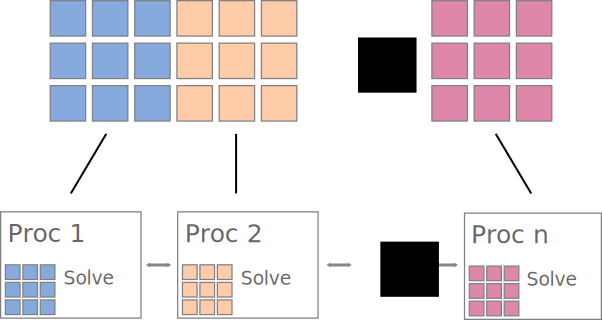
\includegraphics[width=0.5\linewidth]{use-cases/systems/application}
	\caption{A typical parallel application where work is distributed across a number of processes that collectively solve a bigger problem.}
	\label{fig:System: Application}
\end{figure}

\paragraph{System Description:}
A parallel application that utilizes a HPC system to collaboratively solve a large task (for example as listed in \Cref{sec:use cases/climate and weather}).
Many applications use MPI to coordinate and exchange data across compute nodes.
\Cref{fig:System: Application} illustrates how work represented by the colourful boxes is divided and distributed to be handled by multiple processes.

\paragraph{Risks:}
\begin{itemize}
	\item Slow to adopt changes
	%\item May be tightly coupled with post/pre-processing tools, CDOs
\end{itemize}


\paragraph{Subsystems:}
Applications commonly use

\begin{itemize}
	\item Library (Data Description): HDF5/NetCDF, ...  (see \Cref{System: Library})
	\item MPI: Concurrency Control and Communication %(see \Cref{System: MPI})
	%\item (Tooling): Tools either standardized or specific used for pre/post processing.
	%\item In the Future: an earth system middleware (see \Cref{System: ESDM})
\end{itemize}

%%%%%%%%%%%%%%%%%%%%%%%%%%%%%%%%%%%%%%%%%%%%%%%%%%%%
\subsection{System: Software Library (Data Description)}
\label{System: Library}


\paragraph{System Description:}
Climate/NWP codes commonly use libraries to produce portable data formats and also to some extent achieve optimized I/O performance.
Examples are HDF5, NetCDF, Adios, CDI-PIO, XIOS.


\paragraph{Risks:}
\begin{itemize}
	\item APIs may change as the library evolves, requiring Applications and an ESDM to adapt
	\item Abstractions made by library may be inadequate in the future
\end{itemize}


\paragraph{Subsystems:}
We ignore/assume no subsystems for the software libraries for this considerations.
But it is common for a software library to depend on other specialized libraries.




%%%%%%%%%%%%%%%%%%%%%%%%%%%%%%%%%%%%%%%%%%%%%%%%%%%%
\subsection{System: ESDM}
\label{System: ESDM}

\begin{figure}
	\centering
	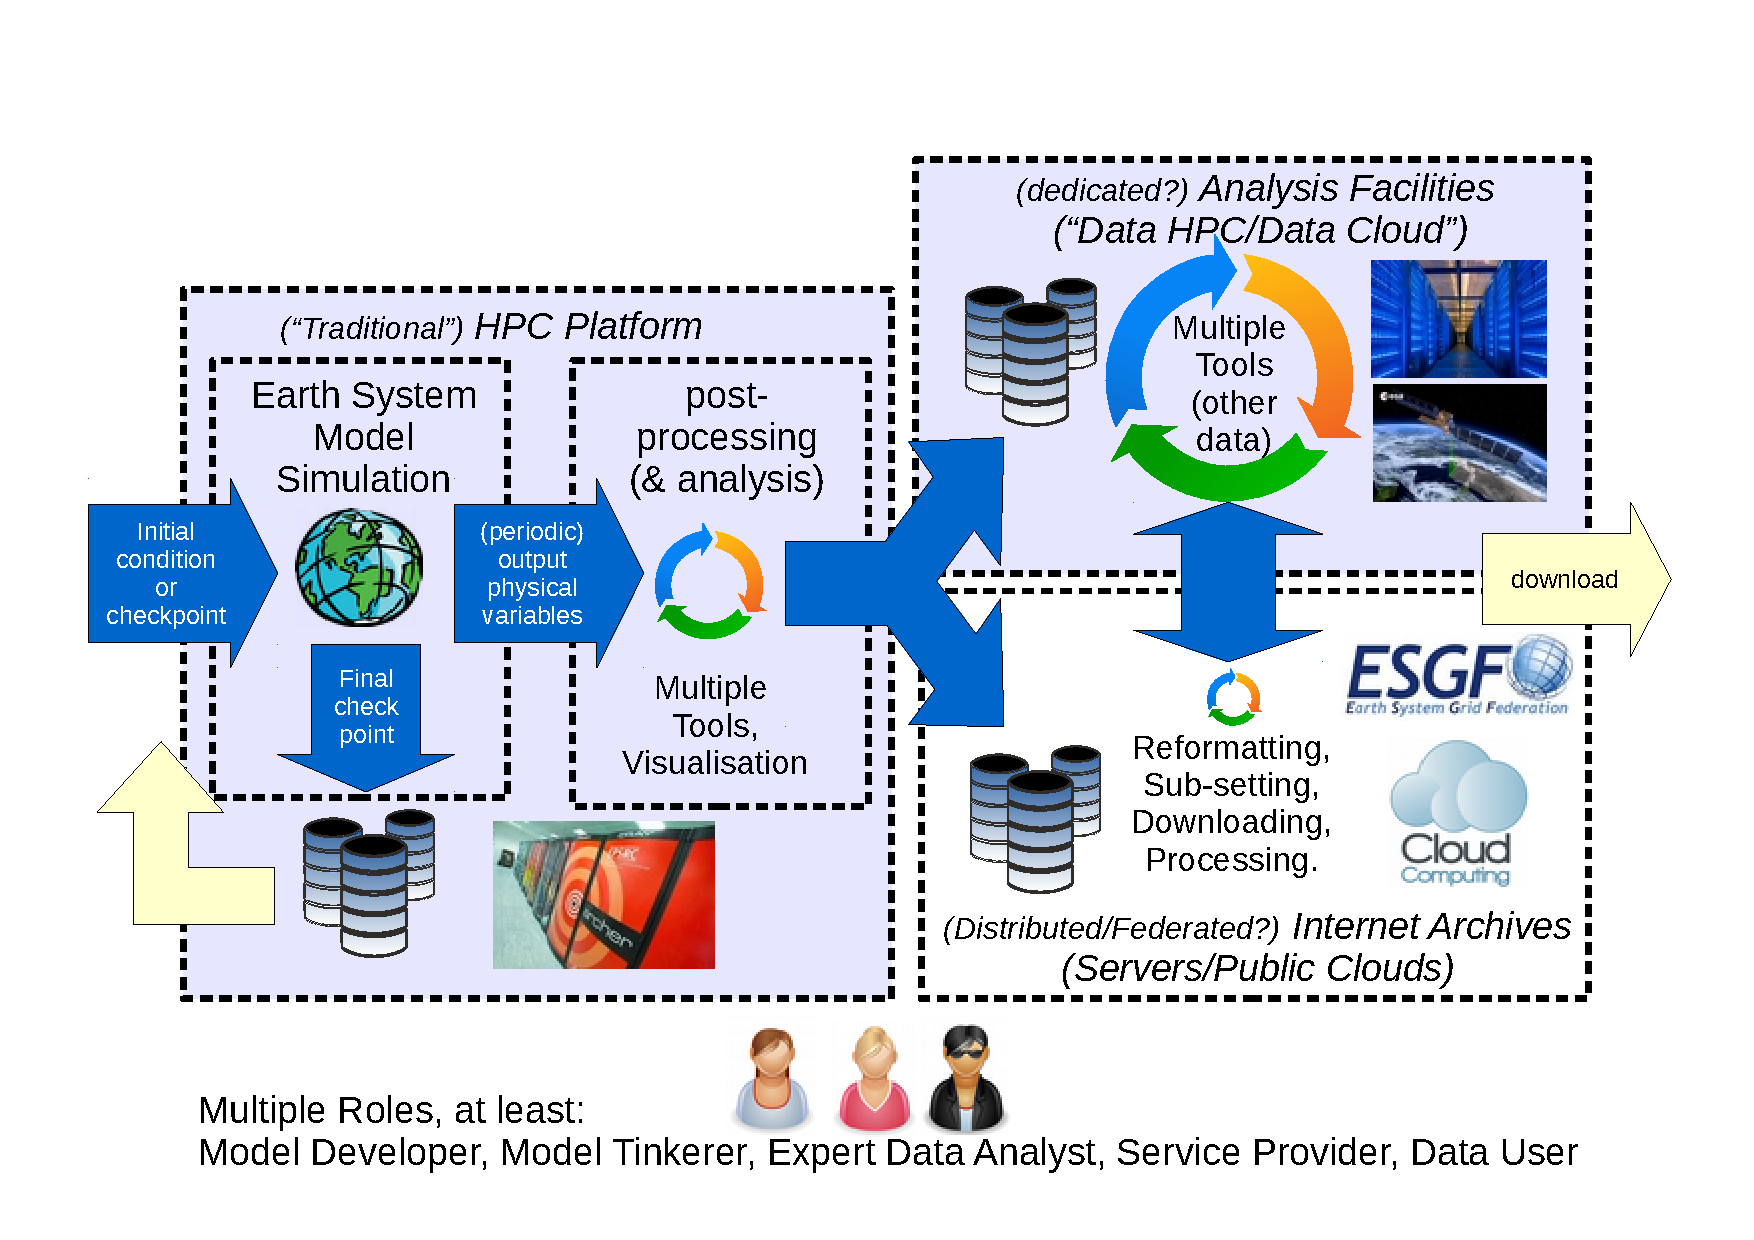
\includegraphics[width=0.75\columnwidth]{3rd/workflow.pdf}
	\caption{Integration and responsible of a ESDM in a climate/weather workflow.}
	\label{fig:system esdm}
\end{figure}


\paragraph{System Description:}
The earth system middleware.
The middleware sits in between the applications and plugins to interact with various data backends.
The middleware decides on the storage backend and exposes characterizations of the data centers as well as assumed data access patterns to be used by backend plugins to realize a fitting segmentation and distribution of domains in the application to storage objects and fragments.
The ESDM manages data in virtual containers and provides a data model (see \Cref{fig:System: Application} and \Cref{fig:system esdm}).
In principle the ESDM in the use cases could be any high-level middleware.


\paragraph{Subsystems:}
We ingore/assume no subsystems except of ESDM backends for the use case discussion.







%%%%%%%%%%%%%%%%%%%%%%%%%%%%%%%%%%%%%%%%%%%%%%%%%%%%
\subsection{System: Job Scheduler}
\label{System: Job Scheduler}

\paragraph{System Description:}
Users submit jobs that run an application to  job schedulers.
The job scheduler will assign resources to a job and start the job.
The ESDM and the job scheduler are assumed to cooperate (see use case in \Cref{uc: simulation}.

\paragraph{Risks:}
\begin{itemize}
	\item No notable risks at this point.
\end{itemize}


\paragraph{Subsystems:}
We ignore/assume no subsystems for job schedulers.





%%%%%%%%%%%%%%%%%%%%%%%%%%%%%%%%%%%%%%%%%%%%%%%%%%
\section{Use Cases}
\label{sec:use cases/use cases}

This section covers the actual use cases as they are addressed by an earth system middleware.
To prevent use cases to become overwhelmingly complex, sub use cases are formulated that can extend or make use of each other.
For example, it is assumed if not otherwise mentioned that the writes/reads handed to a middleware are handled as outlined in \Cref{uc: independent write} and \Cref{uc: independent read} respectively.
The particular examples for independent reads and writes are ignorant of concrete backend.
In a similar fashion, the use case describing how simulations are handled are kept generic, so that a detailed use-case for a POSIX can be swapped with a use-case that describes the handling for e.g., Lustre.
\Cref{uc: simulation} and following address current and anticipated (future) workflows used by weather and climate researchers.

Each use case features a description, involved actors, pre- and post conditions, a flow of events and exceptions.
Application use cases in addition have a priority rating and a description of the domain decomposition on the compute nodes and on storage.
The following list describes the content of each field in detail.


\paragraph{Use-Case Description:} A short description of the use case.

\paragraph{Priority:} A rating on the importance of this use case and a short explanation why.

\paragraph{Actors/Systems:} The involved actors and systems (see\Cref{sec:use cases/actors} and \Cref{sec:use cases/systems}).

\paragraph{Data/Domain Description and Decomposition:} A logical description of the domain and physical domain decomposition across nodes and on the storage system.

\paragraph{Pre-Conditions:} Conditions that have to hold before the use case starts.

\paragraph{Post-Conditions:} Conditions that have to hold after the use case finished.

\paragraph{Related Use-Cases:} A list of other use cases that are related or are used by the use case.

\paragraph{Flow of Events:} A list of actions and events that are triggered as the use case is handled.

\paragraph{Exceptions:} A list of exceptions and failures that may occur and how they are handled.



%%%%%%%%%%%%%%%%%%%%%%%%%%%%%%%%%%%%%%%%%%%%%%%%
\subsection{UC: Independent Write}
\label{uc: independent write}

\paragraph{Use-Case Description:}
A process (e.g., a scientific application or a library) intends to write data using the ESDM interfaces.
The ESDM will determine a mapping and invoke a backend to write data to actual storage targets.
In addition, metadata information for later usage are written or updated.
% (also see \Cref{subsec: technical metadata}).
\Cref{fig:sequence independent write} illustrates the sequence of events in more detail.


\begin{figure}
	\centering
	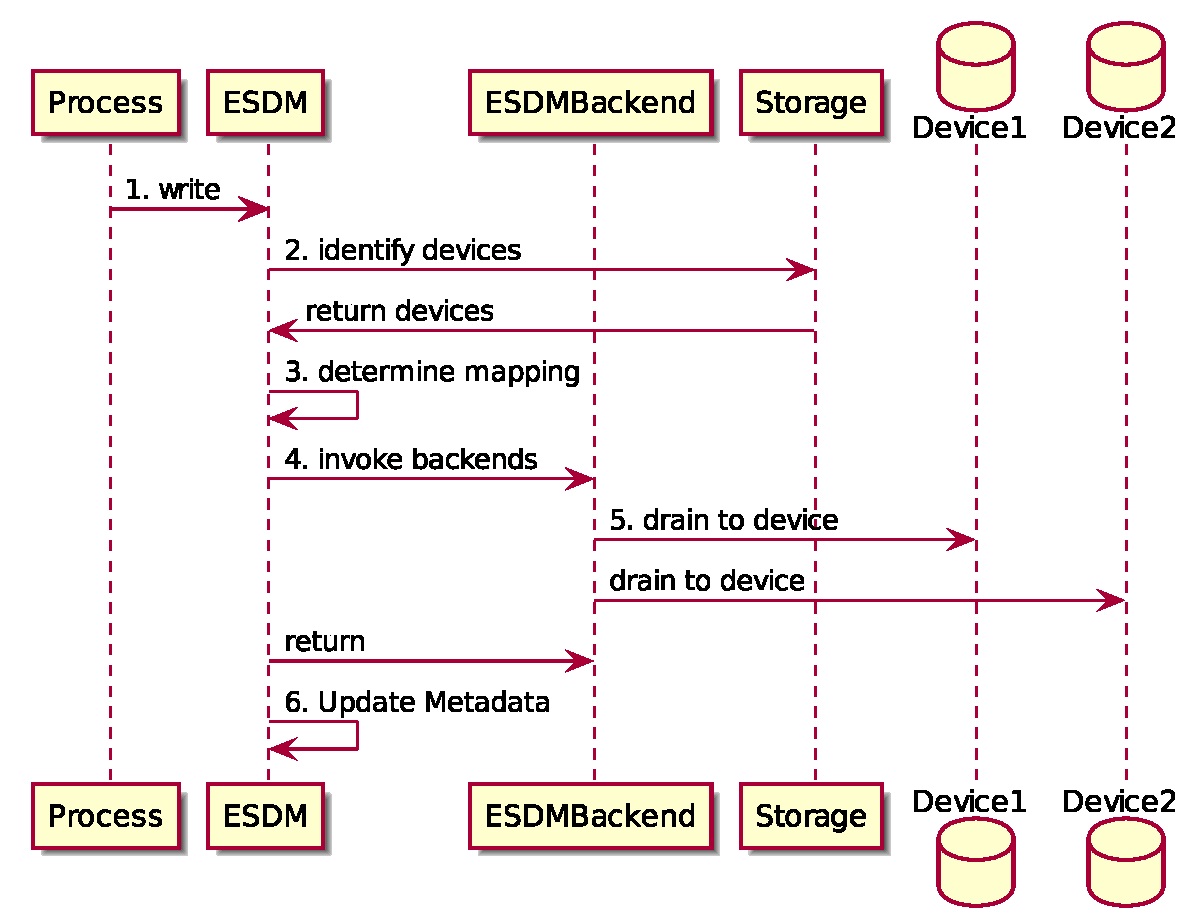
\includegraphics[width=0.7\linewidth]{use-cases/uml/write/sequence.eps}
	\caption{Sequence diagram for handling independent writes. A process issues a write call to the ESDM. The middleware will create a new container if no container already exists. The ESDM collects information about the storage system and determines a domain mapping. The backends responsible for handling a certain storage system are invoked. Multiple different backends may be involved, but each backend is in charge of draining the fragment to a device. Related metadata is updated.}
	\label{fig:sequence independent write}
\end{figure}



\paragraph{Pre-Conditions:}

\begin{itemize}
	\item Parallel application with potentially multiple processes has been started
	\item ESDM has been loaded with a definition of a virtual container used for output
	\item Process: Tries to write data from a single variable to an ESDM virtual container
\end{itemize}

\paragraph{Post-Conditions:}
  \begin{itemize}
  \item Data of the variable has been transferred from process memory to some storage devices
  \item Application can reuse the memory that has been written out
  \end{itemize}

\paragraph{Flow of Events:}
\begin{enumerate}
	\item Process: announces to write a subset of data from a specific domain
	\item ESDM: identifies storage devices to store the data based on system conditions and data properties
	\item ESDM: maps domains to storage backends that will be responsible for the data.
	\item ESDM: initiates writes of data by invoking backends.
	\item Storage backends: drain data onto the storage.
	\item ESDM: updates metadata.
\end{enumerate}

There are many variants of this use case depending on the conditions.






\subsection{UC: Independent Read}
\label{uc: independent read}

\paragraph{Use-Case Description:}
A process (e.g., a scientific application or a library) intends to read data using the ESDM interfaces.
The ESDM has to lookup the metadata and discover available fragments. A domain filling set of fragments has to be found and a storage backend is tasked with reading and reconstructing the requested data from the actual storage targets.
\Cref{fig:sequence independent read} illustrates the sequence of events in more detail.


\begin{figure}
	\centering
	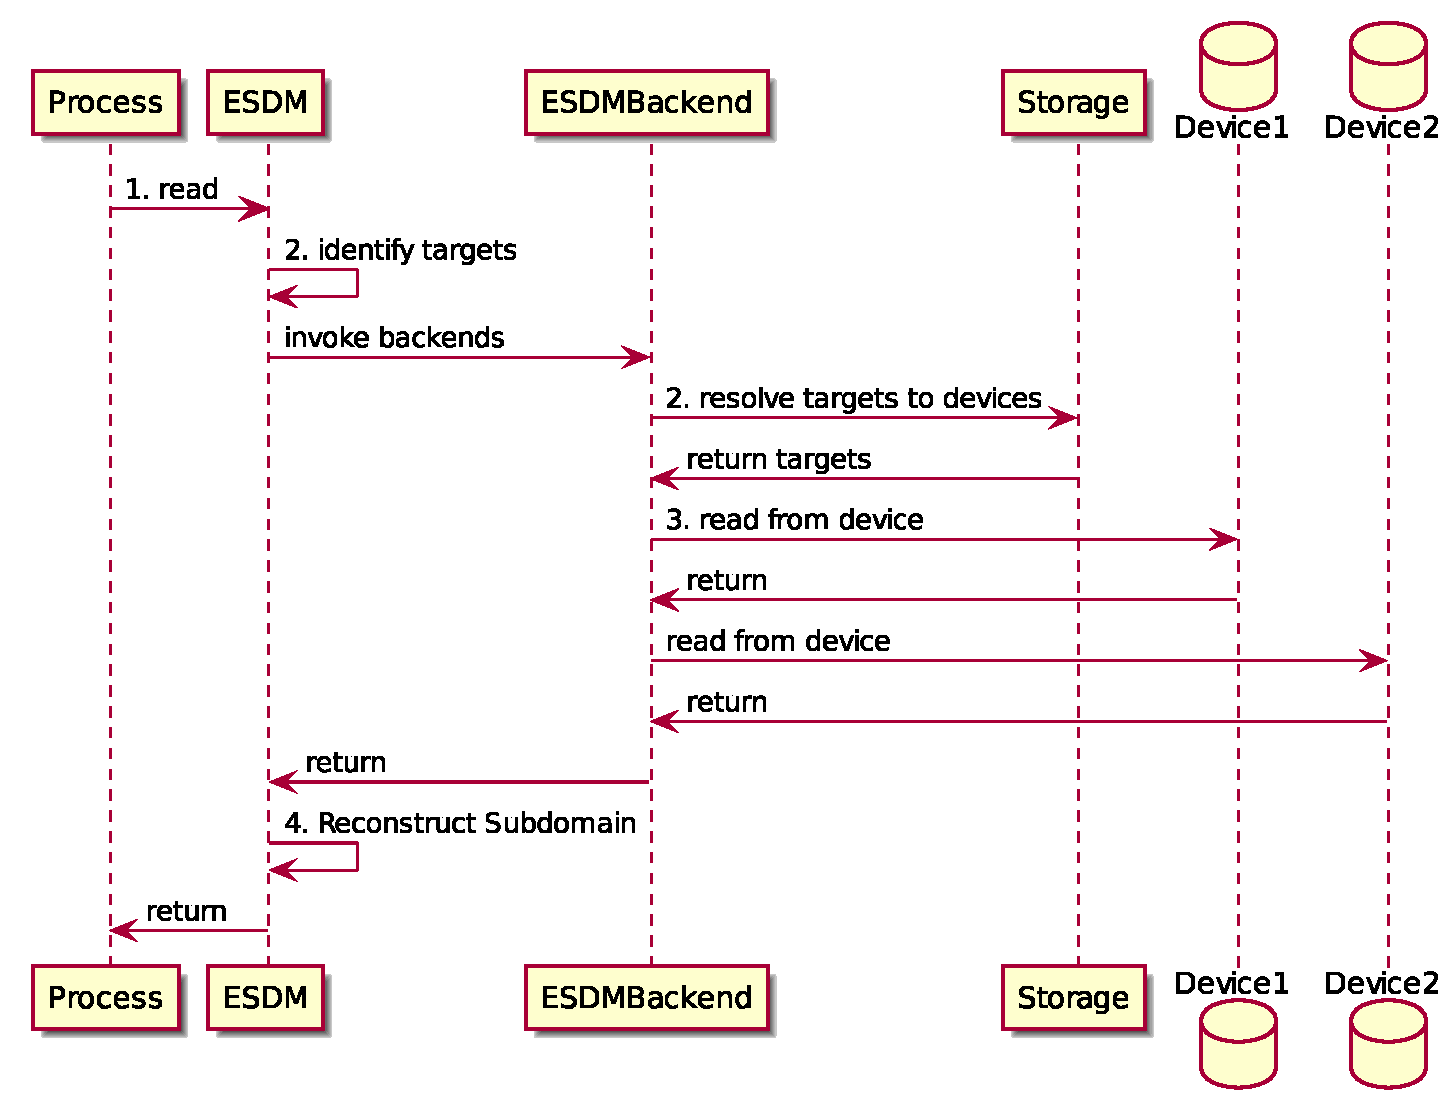
\includegraphics[width=0.75\linewidth]{use-cases/uml/read/sequence.eps}
	\caption{Sequence diagram for handling independent reads. A process issues a read request to the ESDM. The middleware has to lookup related metadata to determine fragments required to reconstruct a domain. An ESDM storage backend will interface with the actual storage systems and fills the request buffer with the reconstructed domain.}
	\label{fig:sequence independent read}
\end{figure}



\paragraph{Pre-Conditions:}

\begin{itemize}
	\item Parallel application with potentially multiple processes has been started
	\item ESDM has been loaded with a definition of a virtual container that contains at least a single variable
	\item Process: tries to read a single variable from an ESDM virtual container
\end{itemize}

\paragraph{Post-Conditions:}
\begin{itemize}
	\item Data of the variable has been retrieved and is now available in the application as part of their domain view.
	\item The data may be cached (e.g., by the ESDM, the OS/Node or the storage system)
\end{itemize}

\paragraph{Flow of Events:}
\begin{enumerate}
	\item Process: announces to read a subset of data from a variable domain
	\item ESDM: identifies storage backends responsible for the data, i.e., map domains to storage backends.
	\item ESDM: initiates read of data on storage.
	\item Storage: provides data
\end{enumerate}






%%%%%%%%%%%%%%%%%%%%%%%%%%%%%%%%%%%%%%%%%%%%%%%%
\subsection{UC: Simulation}
\label{uc: simulation}

Simulations are the main data producers on weather and climate related HPC systems.
Many reading and writing clients are using the persistent storage systems (currently mostly PFS)  to periodically write snapshots that can be used to continue a simulation in case of failure, but more importantly, that is used to analyse the results of simulation runs.

\paragraph{Use-Case Description:}
A user requests a job to be spawned on multiple nodes to perform a simulation of the earth system.
The simulation periodically writes out data for multiple variables, thus the use cases assume a bursty behaviour.
The different variables are written at different frequencies.
For a detailed handling of the different phases refer to the section on the flow of events and \Cref{fig:sequence simulation}.
%\Cref{fig:physical simulation} illustrates the relationships of the different components from an organisational point of view.



\paragraph{Priority:}
High; The standard use-case for simulation driven science in most data centers.

\paragraph{Actors:}
\begin{itemize}
	\item Scientist (initiating the job submission)
	\item Application (a coordinated parallel application, that collaborates collectively on sth.)
	\item Process (the application is realized by N processes. Processes are assumed to perform work independently.
	\item ESDM
	\item Storage devices (could be anything to store, this is a generic use case)
	%\item Supercomputer (physical hardware, offers resources to be used)
	\item Workload manager (responsible to distribute jobs across the cluster hardware)
\end{itemize}


\paragraph{Data/Domain Description and Decomposition:}
A variety of different approaches to structure the logical domains of a model are possible depending on the model implementations.
This use case uses a layered two-dimensional grid in illustrations but other structures are also possible.
\Cref{fig:domain simulation} provides an abstract view to the relation of processes and the grid.

Commonly, a model consists of multiple variables and each variable may vary for a given coordinate over time.
Variables may be written at different frequencies and variables may differ in resolution.
Some simulations use multiple grids, e.g., a region may have a higher resolution than the remaining:

\begin{itemize}
	\item A 2D Grid
	\item Multiple variables
	\item Time series: per timestep a subset of variables is stored each into a single NetCDF file
	\item Potentially multiple domains with different resolutions
	% Containers?
\end{itemize}


For simulations in regard to the middleware we mainly care about how the data is distributed on the nodes, and how it later gets laid out on the storage system:

\begin{itemize}
	\item \emph{Node view:} a subset of the data domain is stored in the main memory of each node.
	%Typically, two copies are necessary: data of the previous time step is used to compute the next time step.
	\item \emph{Storage view:} somehow the data of the variables' domain is serialized into ESD variables and fragments
\end{itemize}

\begin{figure}
	\centering
	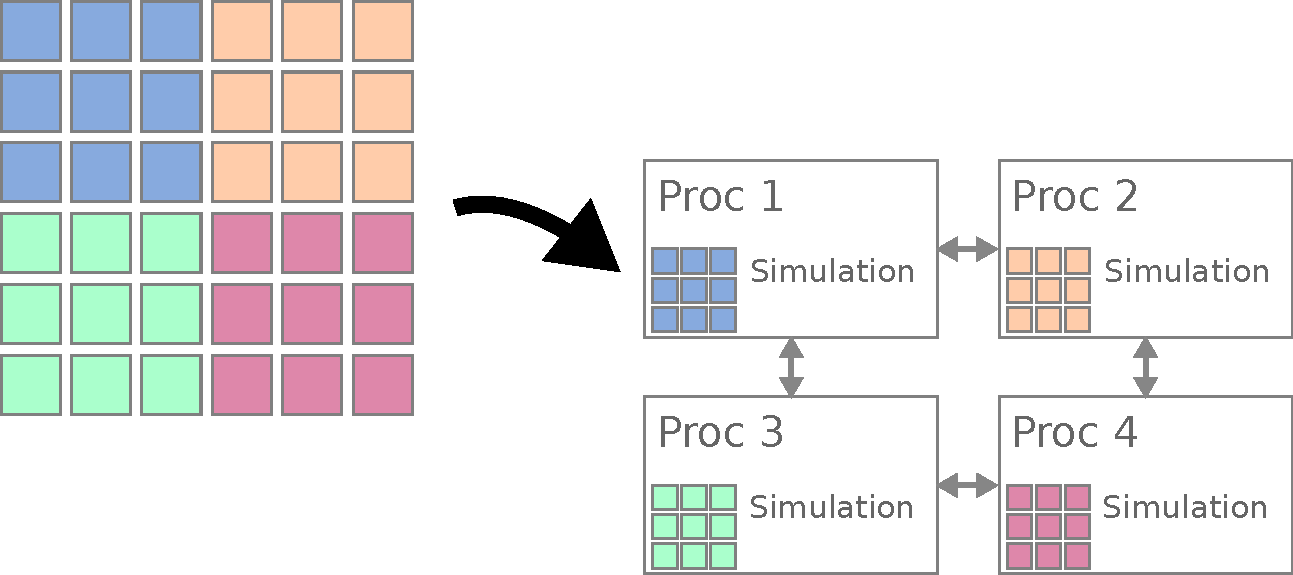
\includegraphics[width=0.5\linewidth]{use-cases/uml/simulation/domain}
	\caption{Example domain decomposition of a logical grid and how the data maybe eventually distributed across multiple processes.}
	\label{fig:domain simulation}
\end{figure}



\paragraph{Pre-Conditions:}

\begin{itemize}
	\item Input data is ready.
	\item The job is about to start by the resource manager.
	\item The user application has credentials to read the input data.
	\item Storage system has adequate health.
\end{itemize}


\paragraph{Post-Conditions:}
\begin{itemize}
	\item Written data has to be in a consistent state; ready to be read by subsequent applications.
\end{itemize}


\paragraph{Related Use-Cases:}
\begin{itemize}
	\item Uses: Independent Read (\Cref{uc: independent read})
	\item Uses: Independent Write (\Cref{uc: independent write})
\end{itemize}

%\todo{This use case most certainly splits into countless variations. Decide on a sensible subset. e.g.: 1) regular grid 2) Icosahedral}


\paragraph{Flow of Events:}
\begin{enumerate}
	\item Scientist: submits a job to run an application with two defined virtual containers, one for IN and one for OUT.
	\item Workload manager: eventually allocates resources to start the job.
	  \begin{itemize}
	  \item Workload Manager: Using the information about the virtual container trigger actions, e.g., pre-staging of input data into local storage hardware or reserving bandwidth and storage space on output devices with limited capacity such as NVRAM.
	  \end{itemize}
	\item Application opens the IN container (read-only) in collective mode.
	\item ESDM: optimizes the container for read mode (optionally done during staging mode).
	\item Application opens the OUT container (write-only) in collective mode, allocate known space if necessary.
	\item ESDM: prepares the container for write mode.
	\item Application: announces to read initial simulation data.
	\item See UC: Read, it might be collective (better) or independent.
	\item Application: runs the time series of computation:
	\begin{enumerate}
		\item Process: Read auxiliary data (if necessary), see UC: Read
		\item ESDM: identifies storage devices
		\item Process: Computes (and communicates)
		\item Process: Writes subset of variables, see UC: Write
	\end{enumerate}
	\item Application: closes the container.
	\item Application: finishes computation and terminates.
	\item Workload Manager: free the resources, manage evtl. stage occupied local storage resources.
\end{enumerate}


\paragraph{Exceptions:}
\begin{enumerate}
	%\item Everything works as expected the application completes N timesteps and writes M snapshots.
	\item Applications crashes between two time steps or before regular termination.
	\item Consistency of virtual container is faulty.
	\item Network problems (Link Failure, Switch Failure) lead to premature termination of job. ESDM has to clean up references to incomplete container.
	\item A failure occurs the last snapshot does not complete. As a result the index for the last snapshot maybe broken. The ESDM has clean up unreferenced fragments.
\end{enumerate}


\begin{figure}
	\centering
	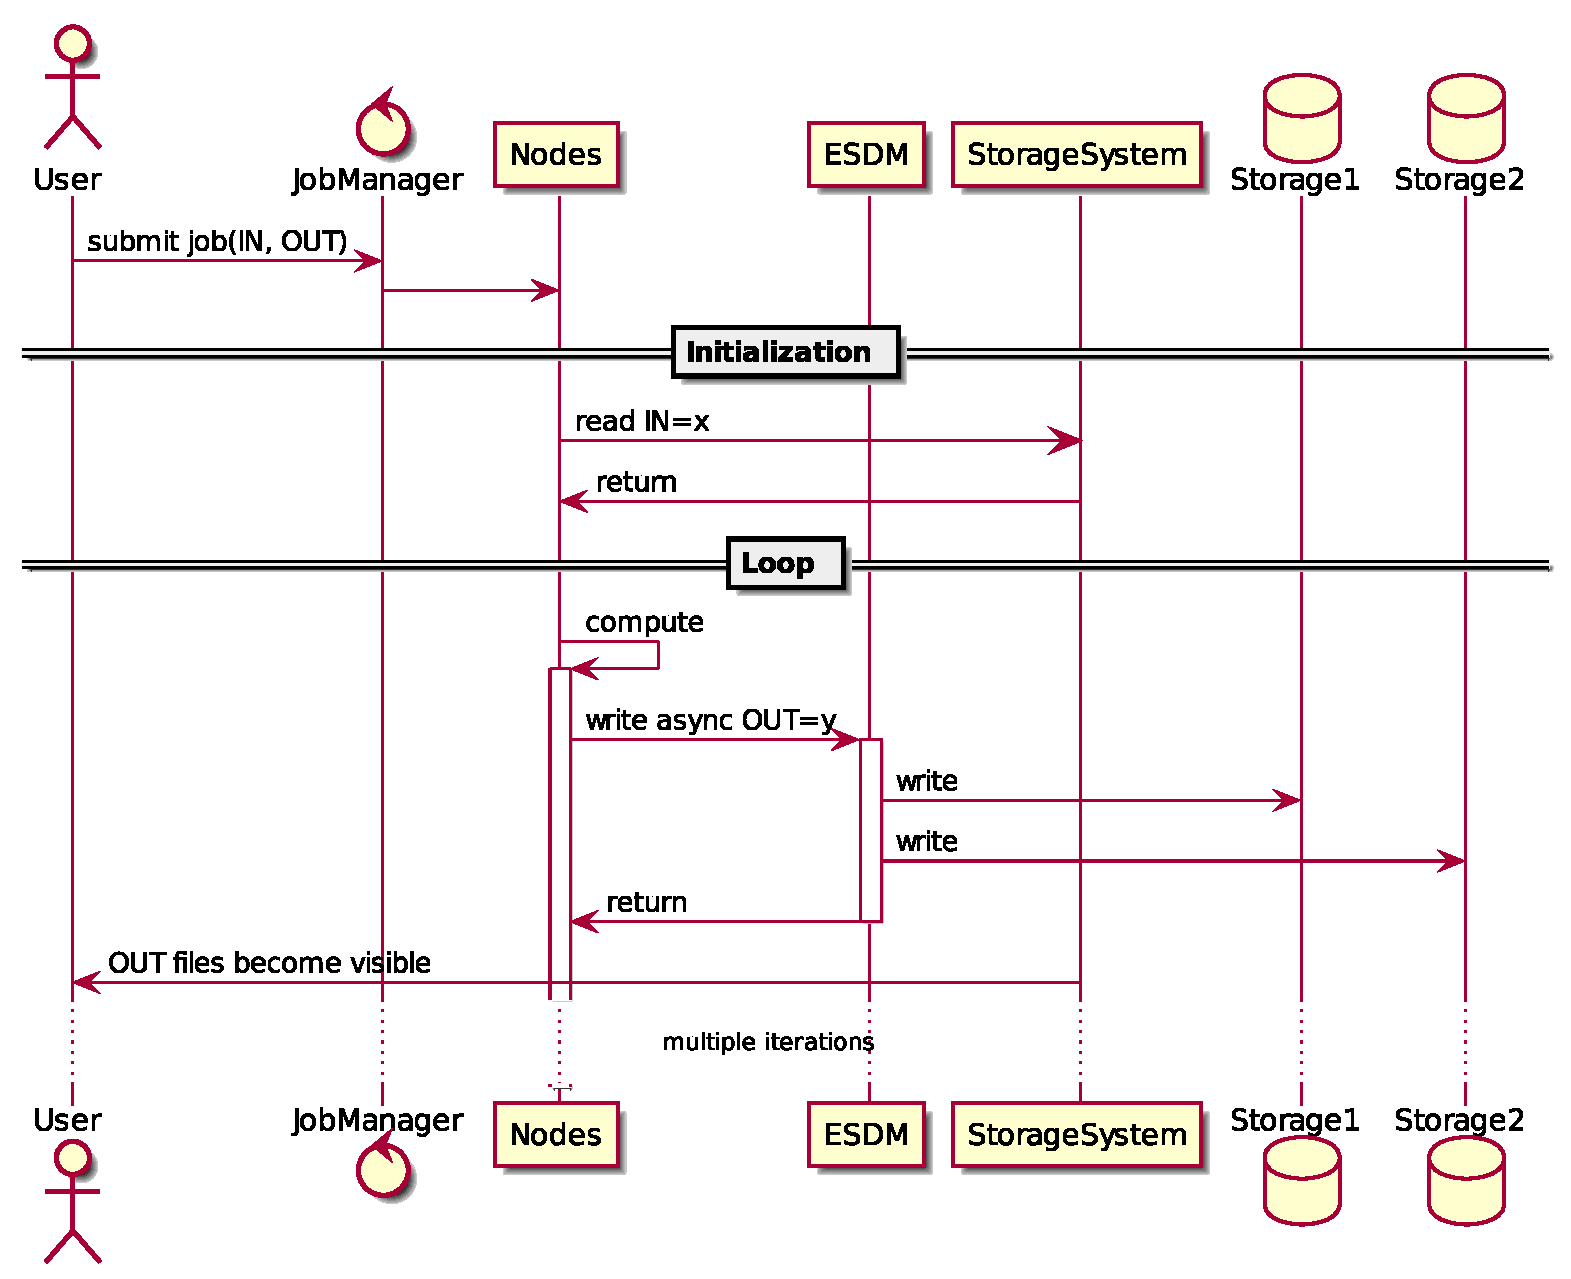
\includegraphics[width=\linewidth]{use-cases/uml/simulation/sequence.eps}
	\caption{Sequence diagram for the simulation use case. A user submits a job with IN and OUT destinations specified. A job manager will spawn the actual job by allocating nodes and ordering to start the application code on each node. Usually simulations need to read in a set of initial conditions. It will then iteratively compute one time step after another, while occasionally (usually at fixed frequencies which may vary per variable) writing snapshot data to be used during analysis or to restart an interrupted simulation.}
	\label{fig:sequence simulation}
\end{figure}


%\begin{figure}
% 	\centering
% 	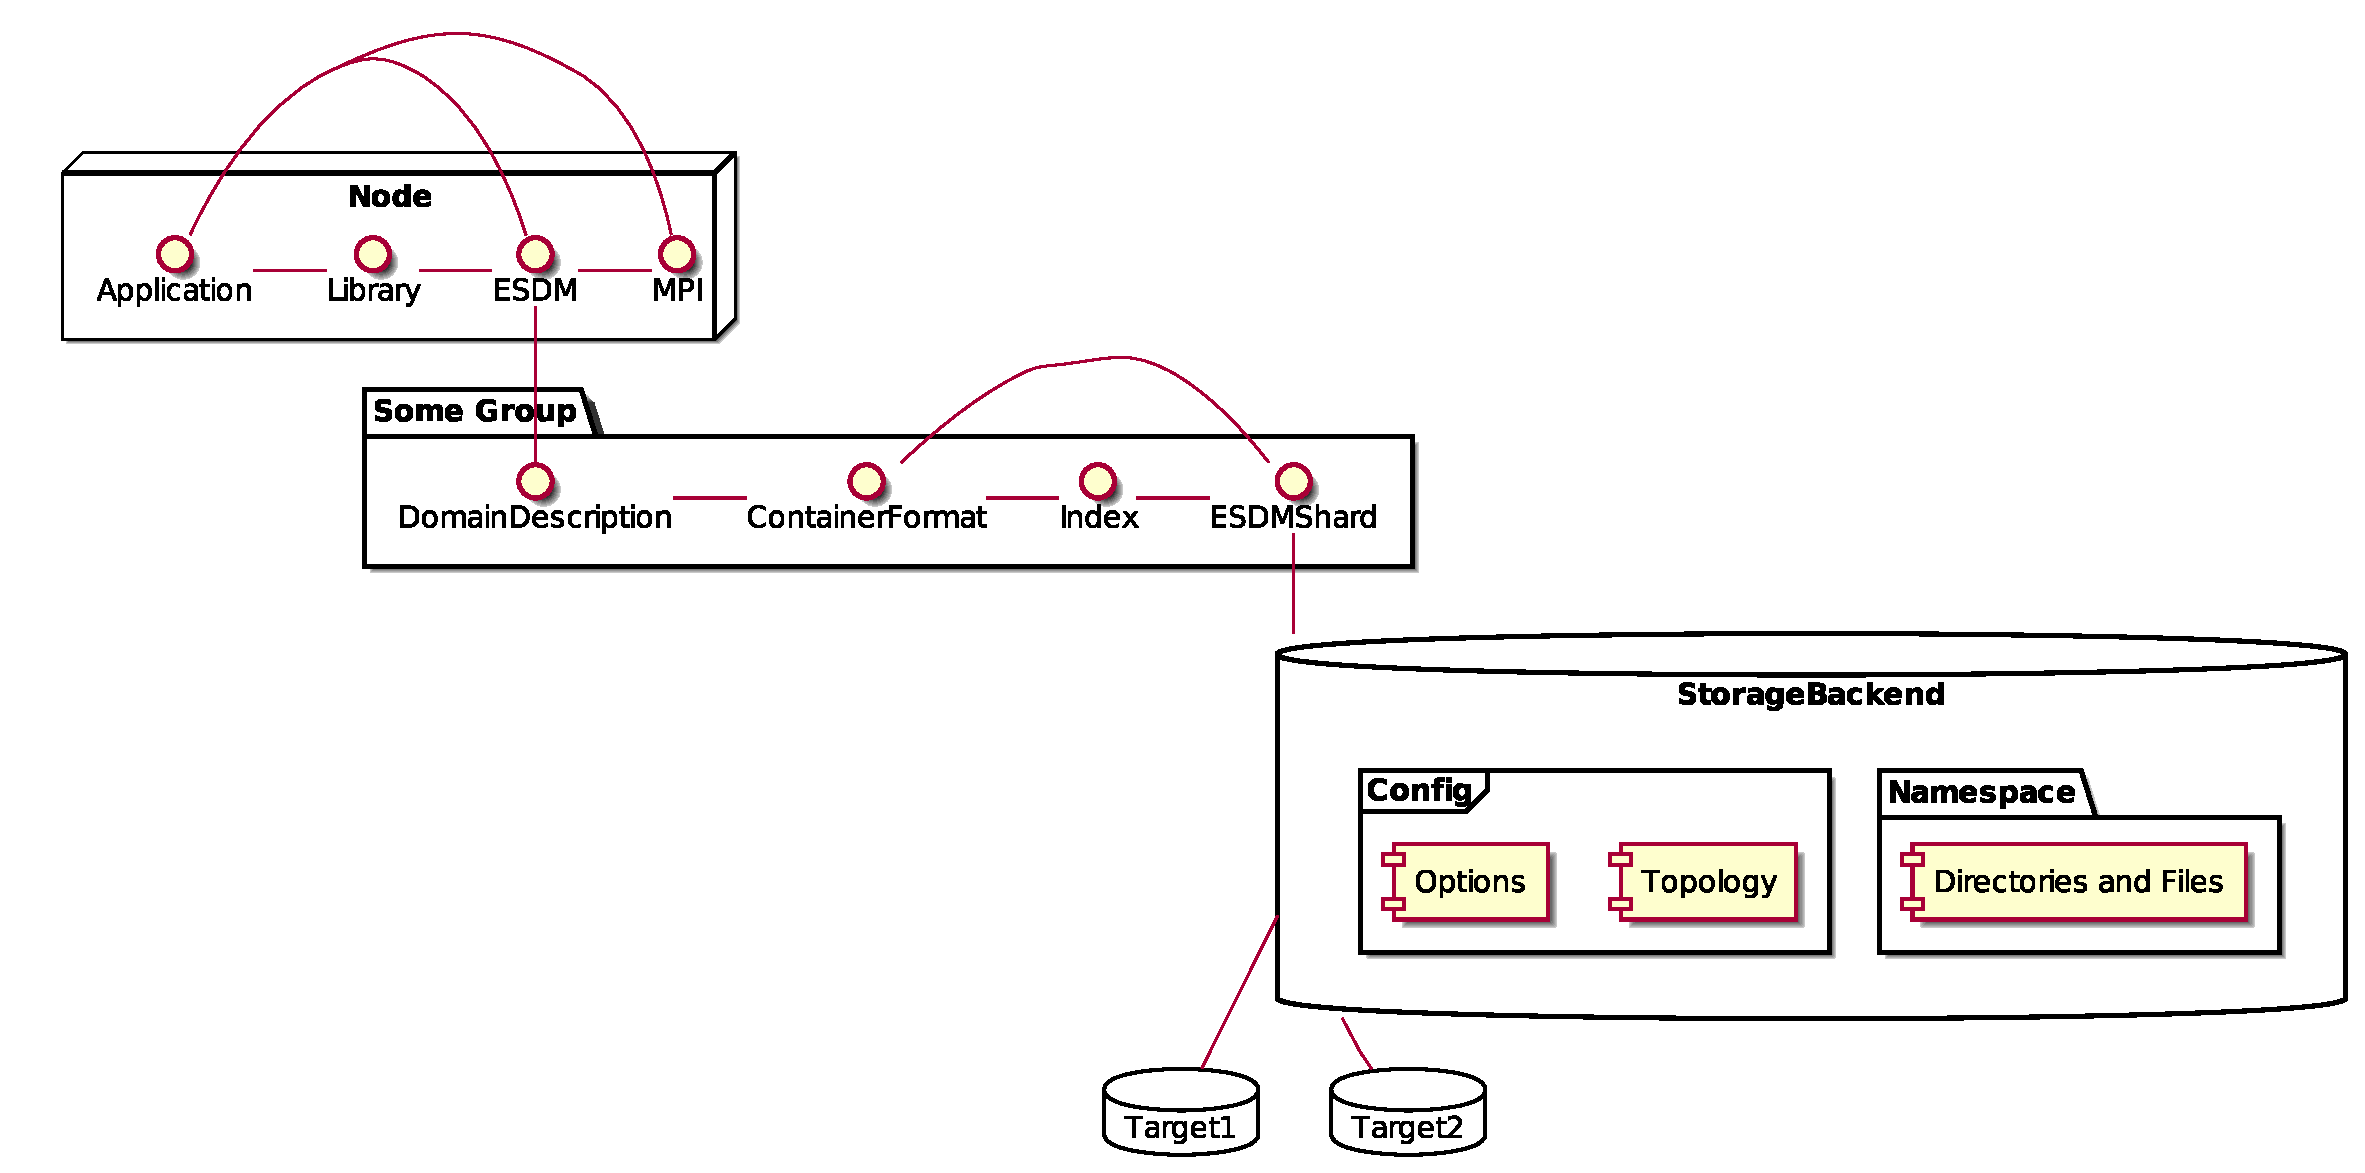
\includegraphics[width=\linewidth]{use-cases/uml/simulation/participants.eps}
% 	\caption{View of participants and their relations. An application, is likely to interface with the ESDM only indirectly through a library. Applications as well as the ESDM coordinate using MPI. Each node running the simulation is has loaded the application code, libraries, the ESDM and MPI as well as memory that is managed by each of these. Within the ESDM different submodules are active that handle the domain description, interpret the container format and ESDM fragments. For the storage backend, an administrator has to provide configuration information such as the topology and the namespace organisation.}
% 	\label{fig:physical simulation}
% \end{figure}







%%%%%%%%%%%%%%%%%%%%%
\subsection{UC: Pre/Post Processing on a existing Data}
\label{uc: pre + post processing}

Before a simulation can run, input data from satellites, weather stations and other sources has to be converted into a representation that matches the grid of the simulation.
Similarly, simulations output a lot of raw data to be flexible to perform at simulation-time unexpected analysis.
Pre- and post processing jobs are therefore an integral part of the workload mix at supercomputing sites but also on smaller local installations.


\paragraph{Use-Case Description:}
A user submits a pre/post processing job to the workload manager requiring to read datasets from one or more input sources.
Ideally, the task is described using a common tool or a framework for data transformations (e.g. CDO).
There are countless possibilities for type of calculations performed and for the regions that need to be accessed in the logical domain (see \Cref{fig:domain pre + post processing})
Many analysis workloads access time series data, thus require to access similarly-structured files with the same pattern.
\Cref{fig:sequence pre + post processing} illustrates the sequence of events in more detail.

\paragraph{Priority:} High, Researchers routinely have to perform pre/post processing

\paragraph{Actors:}
\begin{itemize}
	\item Scientist
	\item Pre/Post Processing Application (e.g. CDO)
	\item Supercomputer
	\item ESDM
\end{itemize}


\paragraph{Data/Domain Description and Decomposition:}
In alignment with the other use cases, a Cartesian grid is assumed but many other grids are in principle handled in similar manner.
\Cref{fig:domain pre + post processing}
%\todo{text in figure: stripe size 5- may be stride you mean?  Some systems call it stride some call it stripe.. On instance with lustre wich uses strips in the same context as in the picutre..  https://www.nics.tennessee.edu/computing-resources/file-systems/lustre-striping-guide }
 illustrates the logical decomposition, an example serialization and the distribution across a storage system.
The producing application decided for which access pattern the serialization is favourable, in many situations the provided serialization is suboptimal for the transformation.


\begin{figure}
	\centering
	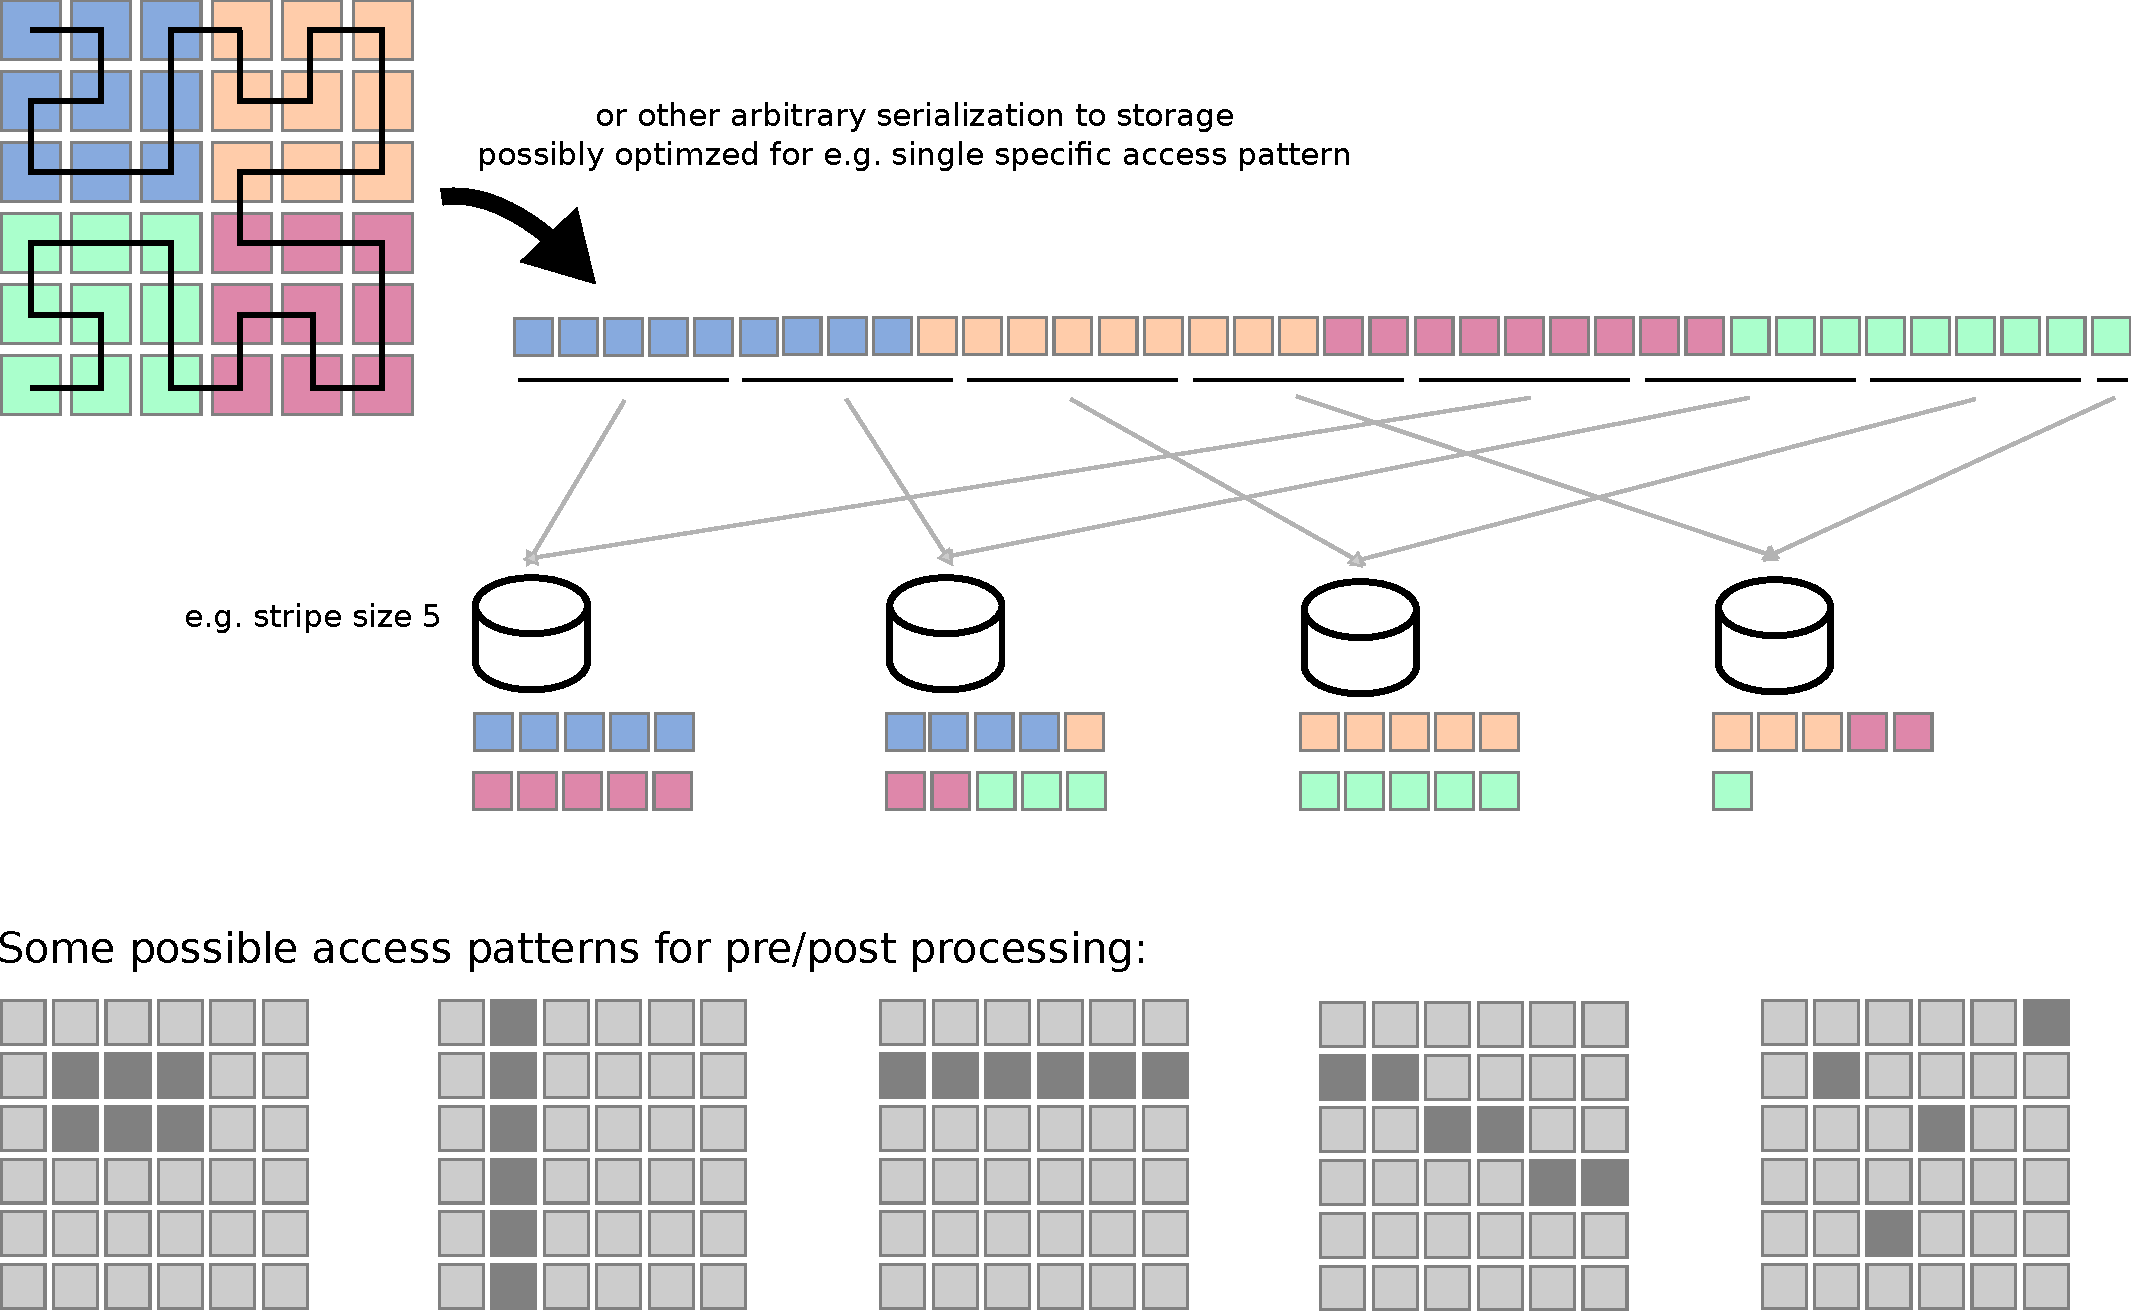
\includegraphics[width=\linewidth]{use-cases/uml/prepost-processing/domain}
	\caption{The logical domain view, a serialization and how it is striped across a storage system. The grey grids below illustrate possible access patterns, but the layout on storage is not optimal for any of the shown access patterns. }
	\label{fig:domain pre + post processing}
\end{figure}


\paragraph{Pre-Conditions:}
\begin{itemize}
	\item Dataset is available via ESDM (because of producer termination or epoch)
	\item The dataset maybe available, but may have suboptimal fragmentation.
	\item A common description/framework for post processing is used (e.g. CDO)
\end{itemize}

\paragraph{Post-Conditions:}
\begin{itemize}
	\item The pre/post processing region of interest result is accessible by the user.
	\item The dataset container is improved by additional indexes or additional fragments for faster access next time.
\end{itemize}

\paragraph{Related Use-Cases:}
\begin{itemize}
	\item Uses: Independent Read (\Cref{uc: independent read})
	\item Uses: Independent Write (\Cref{uc: independent write})
\end{itemize}


\paragraph{Flow of Events:}
\begin{enumerate}
	\item Scientist: submits a post processing job, multiple virtual containers for INPUT and OUTPUT may be specified.
	\item Workload Manager: eventually allocates resources and starts the job.
	\item Pre/Post processing may open multiple files one after another (e.g. time series)
	\begin{enumerate}
	\item Process: opens the INPUT  (see UC: Read \Cref{uc: independent read})
	\item Process: performs transformation or analysis (e.g. compute average)
	\end{enumerate}
	\item Process: Writes a transformed dataset (see UC: Write \Cref{uc: independent write})
	\item Process: Possibly, creates plot or film of analysis.
\end{enumerate}


\begin{figure}
	\centering
	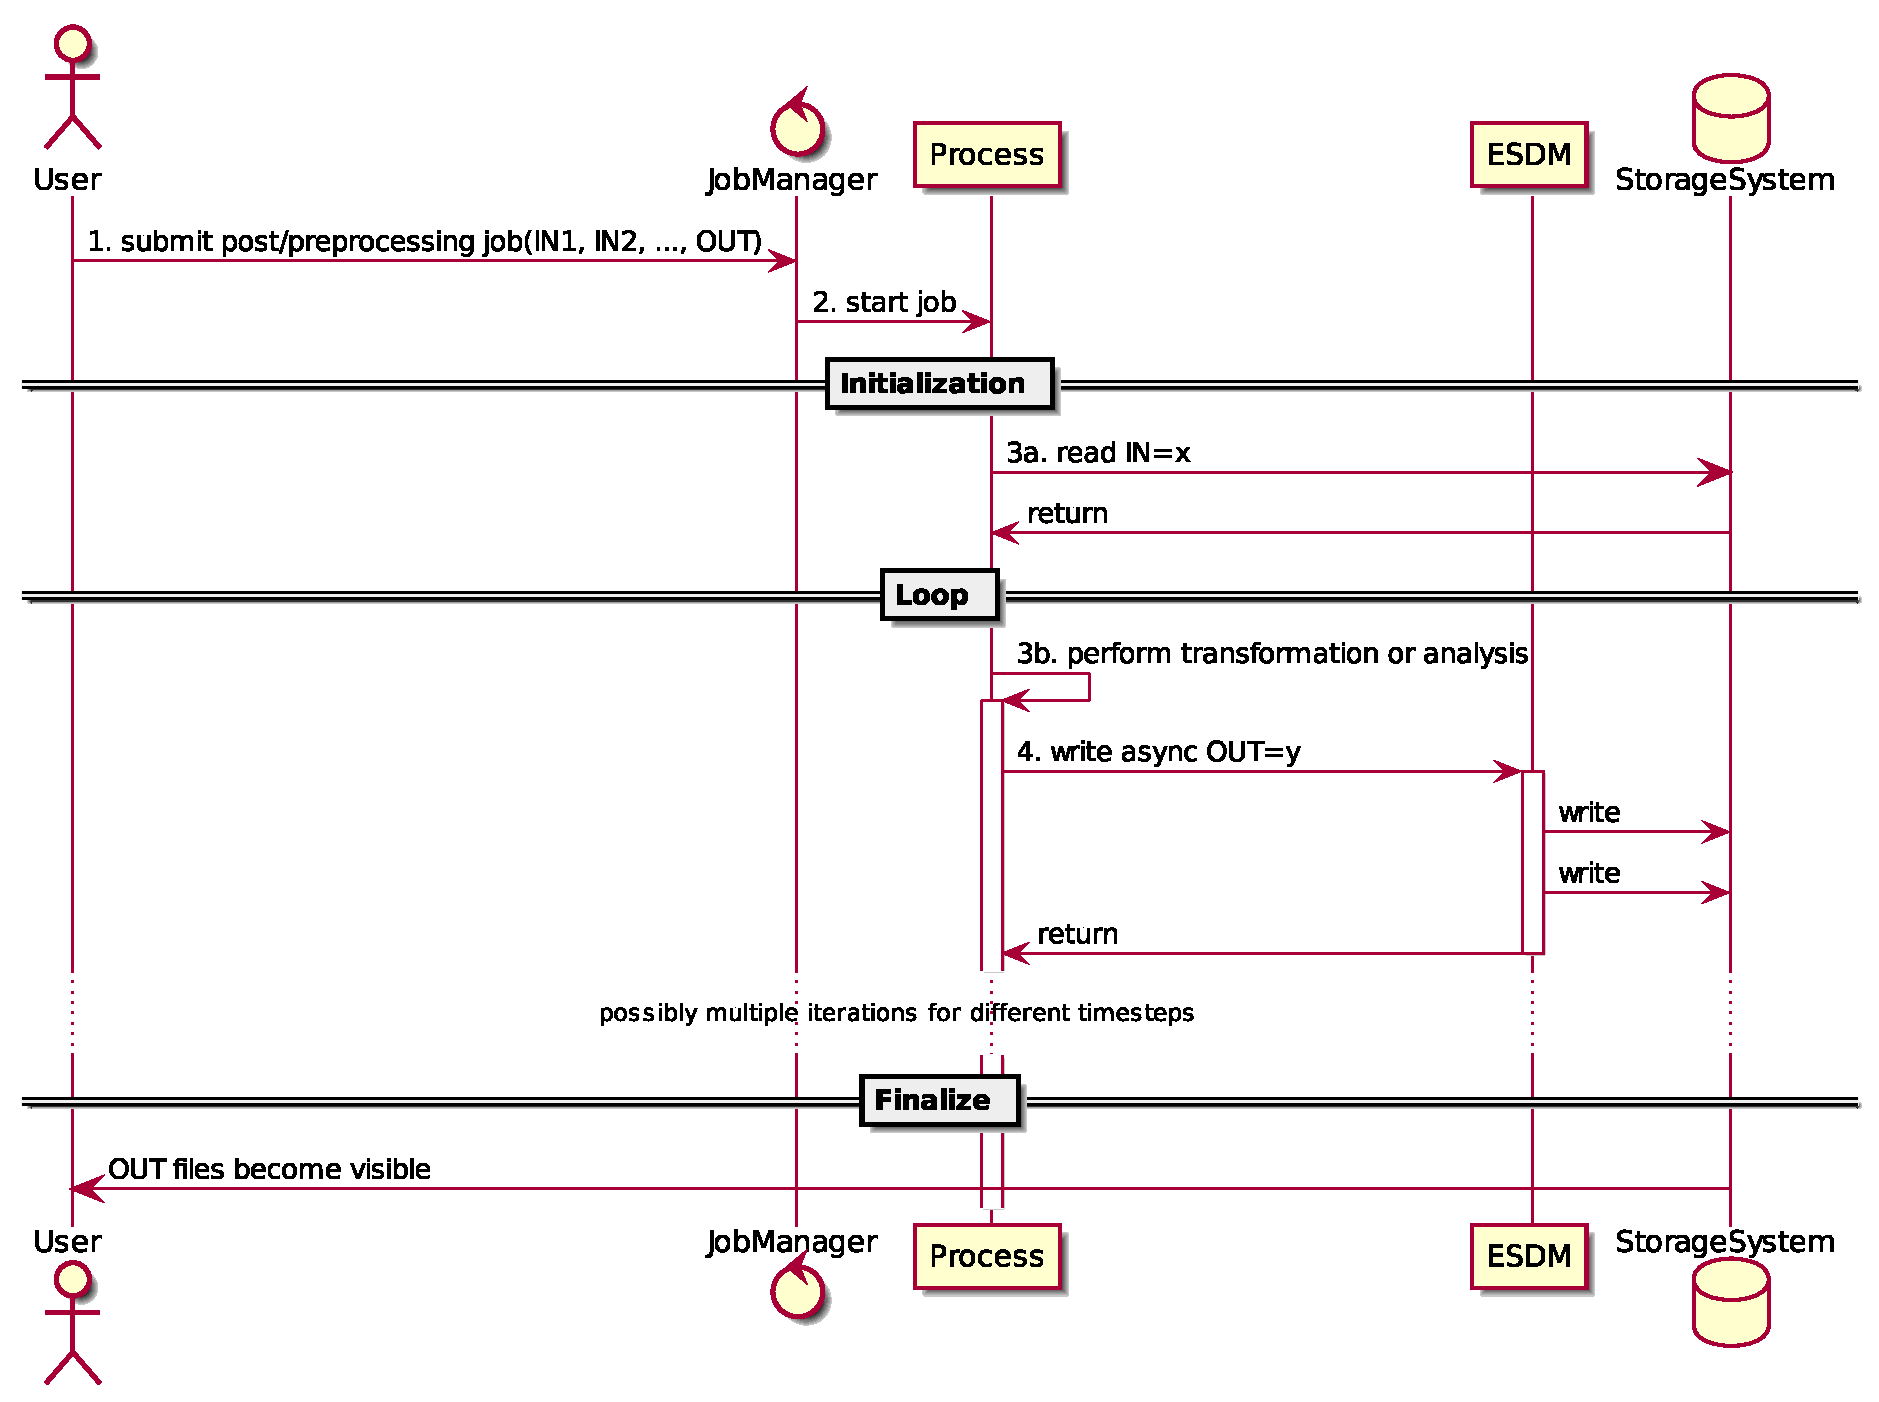
\includegraphics[width=\linewidth]{use-cases/uml/prepost-processing/sequence}
	\caption{Sequence diagram for the flow of events for a stand-alone pre/post processing task. Depending on the analysis task, no output may occur until all data from a time series was gathered.}
	\label{fig:sequence pre + post processing}
\end{figure}



\paragraph{Exceptions:}
\begin{enumerate}
	\item  Requiring to ensure clean up of unreferenced/inconsistent data is inherited from Read/Write use cases (see \Cref{uc: independent read} and \Cref{uc: independent write})
\end{enumerate}



%
%\todo{
%	Domain, subdomain, coordinates
%
%	Layout component index:
%	- Coordinates are in fragment Z; does NOT tell where in the fragment
%	- Optimize number of fragments to query
%	- Performance predictor für jedes PFS ?	\item
%
%	PFS index:
%	- File: sequence(metadata + pointer to last metadata + data ), index (with pointer to all metadata blocks)
%	Mapping from multidimensional coordinates to byte offset and array
%	Many different representations are possible
%
%	Potentially more than one fragment into one file (optimize metadata for millions of procs).
%
%}
%



%%%%%%%%%%%%%%%%%%%%%%%%%%%%%%%%%%%%%%%%%%%%%%%
\subsection{UC: Concurrent Simulation and Post processing for Pipelines/Workflows}
\label{uc: pipeline}

For weather prediction it is common to have post processing pipelines responsible for the generation of value-added services.
In expectancy of formal definition of workflows and increased use of containerization this use case describes how an ESDM would need to realize automatic post-processing as soon as data becomes available.


\paragraph{Use-Case Description:}
A processing pipeline is set up that constantly receives new input data, for example measurement data from a satellite system.
Periodically, the most recent satellite data is fed to a simulation as input (see \Cref{uc: simulation}).
As simulations write snapshots, value-added products are generated in post processing steps.
For example in a NWP setting warnings or a weather forecast (compare \Cref{sec:use cases/climate and weather}).
\Cref{fig:sequence pipeline} illustrates the sequence of events in more detail.




\paragraph{Priority:}
Low - Not in scope of project to integrate with in-situ post processing tools.
Also other systems such as the workload manager need to be adapted to support this.


\paragraph{Actors:}
\begin{itemize}
	\item Scientist
	\item Application
	\item Supercomputer
	\item ESDM
	\item Pre/Post Processing Framework
\end{itemize}


\paragraph{Data/Domain Description and Decomposition:}
The input data may be in various formats with a domain layout that is not optimal for the simulation.
For simplicity, conversion steps are omitted in the description, but if necessary a transformation would correspond to UC: Pre/Post Processing (see \Cref{uc: pre + post processing}).
\Cref{fig:domain workflow} illustrates an observation system that provides data in portable container format (could also be an ESDM container).
The observation data is then used as initial conditions for a simulation, the domain decomposition and resulting output matches the description in UC: Simulation (see \Cref{uc: simulation}).
Finally, the output data is post processed for which the domain description, again, corresponds to UC: Pre/Post Processing (see \Cref{uc: pre + post processing}).


\begin{figure}
	\centering
	\includegraphics[width=\linewidth]{use-cases/uml/pipeline/domain}
	\caption{Illustration of the domain and a possible pipeline. New observational data is constantly added, and then used in simulations. The simulation output is then used by post processing tasks to compile specific forecasts and warnings.}
	\label{fig:domain workflow}
\end{figure}




\paragraph{Pre-Conditions:}
\begin{itemize}
	\item Sufficient resources to start simulations and post processing workloads available.
	\item A pipeline is provided in a machine-readable format.
	\item Simulation preconditions as described in UC: Simulation apply (\Cref{uc: simulation})
	\begin{itemize}
		\item Input data is ready.
		\item The job is about to start by the resource manager.
		\item The user application has credentials to read the input data.
		\item Storage system has adequate health.
	\end{itemize}

\end{itemize}


\paragraph{Post-Conditions:}
\begin{itemize}
	\item Post processing can compute results as soon as an epoch completes.
	\item Combined task is hopefully faster than traditional approaches (generate, write, [read, transform, write], read, postprocess, write result)
\end{itemize}


\paragraph{Related Use-Cases:}
\begin{itemize}
	\item Uses: Independent Read (\Cref{uc: independent read})
	\item Uses: Independent Write (\Cref{uc: independent write})
	\item Adapts: Simulation (\Cref{uc: simulation})
	\item Adapts: Pre/Post processing on an existing Data (\Cref{uc: pre + post processing})
\end{itemize}


\paragraph{Flow of Events:}
\begin{enumerate}
	\item Observation System: Observations are constantly stored and timestamped.
	\item ESDM: handles storage on storage system and potentially transforms data as needed by pipeline/workflow.
	\item Workload Manager: periodically allocate resources to spawn new jobs with most recent data
	\begin{enumerate}
		\item Application: A simulation is started as outlined in UC: Simulation (\Cref{uc: simulation})
		\item Application: opens the INPUT (see UC: Read \Cref{uc: independent read})
		\item ESDM: Serves the input. This is another time for ESDM to transform data.
		\item Application: Loop
			\begin{enumerate}
				\item Application: writes subset of variables
				\item ESDM: makes data available to post processing immediately (e.g., inform workload manager to schedule post processing job)
				\item ESDM: writes snapshot asynchronously
			\end{enumerate}
	\end{enumerate}
	\item Repeat.
\end{enumerate}

\begin{figure}
	\centering
	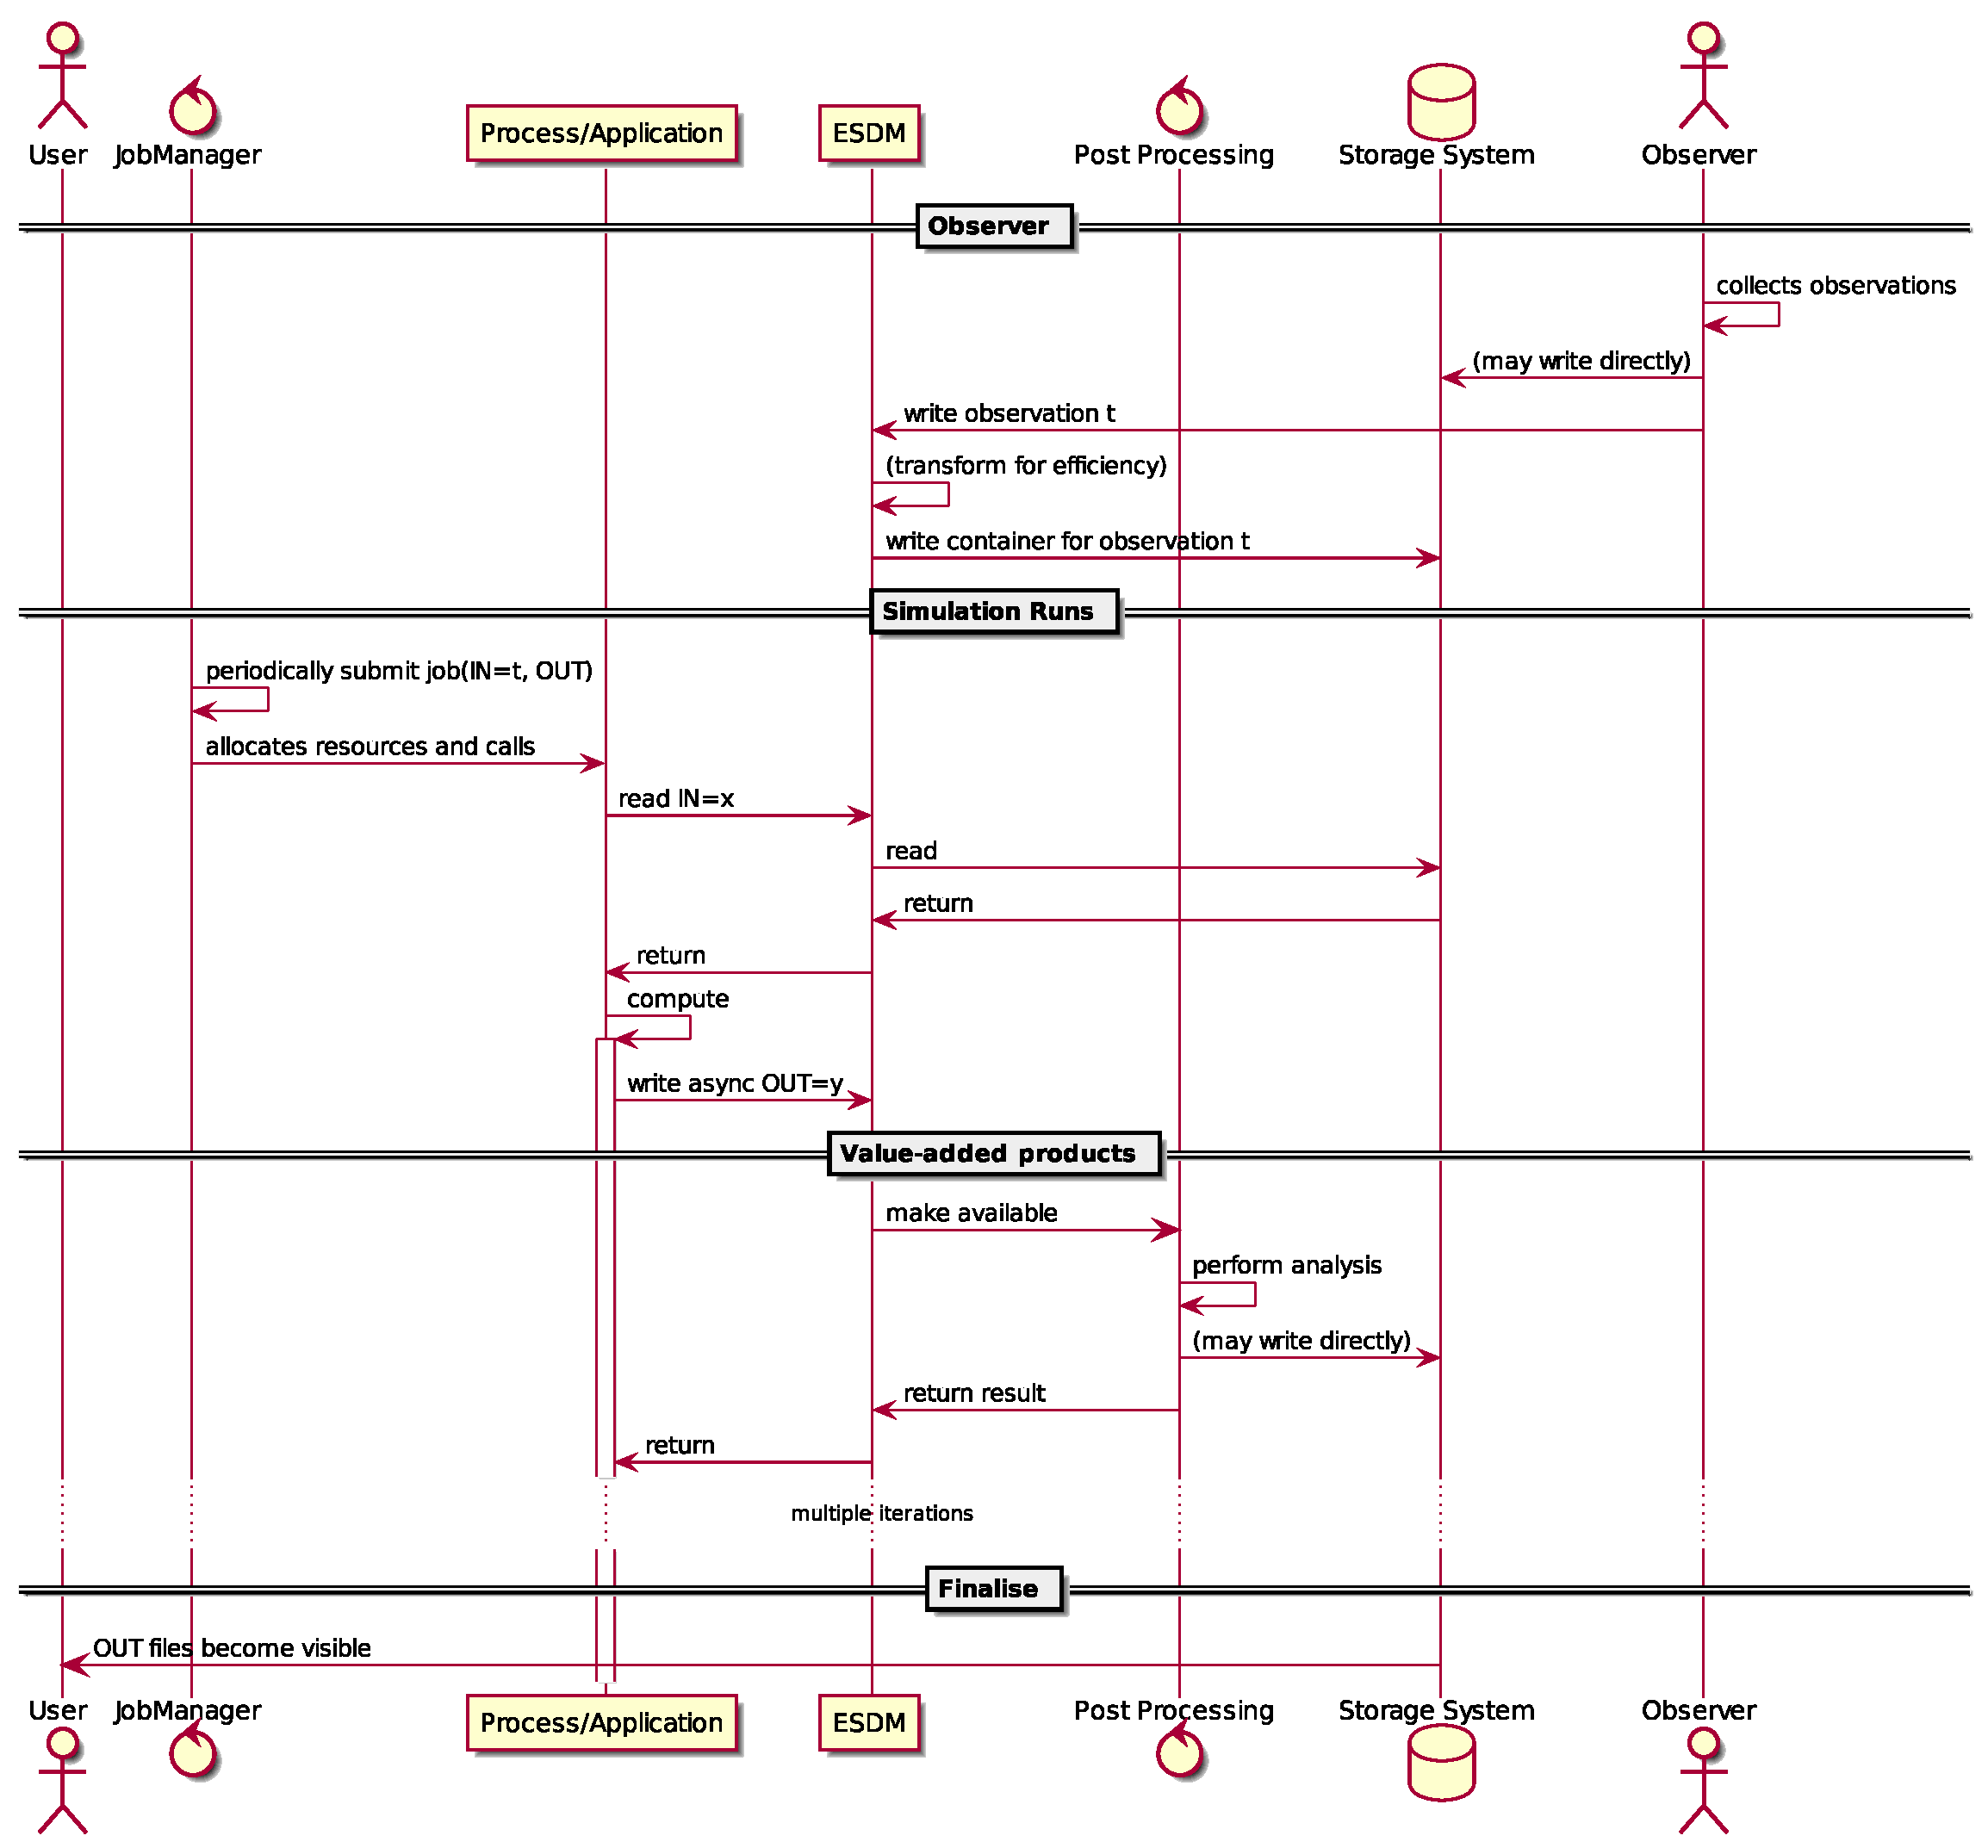
\includegraphics[width=\linewidth]{use-cases/uml/pipeline/sequence.eps}
	\caption{Sequence Diagram for Concurrent Simulation and Post processing for Pipelines/Workflows}
	\label{fig:sequence pipeline}
\end{figure}




\paragraph{Exceptions:}
Multiple failure modes are possible, but they are all inherited by the used use cases only may require cleaning up inconsistent/incomplete fragments and containers:

\begin{enumerate}
	\item Simulations can fail (see UC: Simulation \Cref{uc: simulation})
	\item Pre/Post Processing of existing data may also fail (see \Cref{uc: pre + post processing})
\end{enumerate}


%%%%%%%%%%%%%%%%%%%%%%%%%%%%%%%%%%%%%%%%%%%%%%%
\subsection{UC: Simulation + In situ post processing}
\label{uc: simulation + in-situ + post processing}

A common problem with post processing applications is that data is first written to storage, just to be read again from another consumer for post processing.
This unnecessarily stresses the storage system, because if it is known in advance that an average for an area needs to be calculated, then the generating application can notify or perform the post processing on the node where the data is already present.


\paragraph{Use-Case Description:}
A job is spawned on multiple nodes which collectively run a simulation of the earth system (see \Cref{uc: simulation}).
The job contains information about necessary post processing steps.
Alternatively, the job maybe part of workflow, and the post processing steps are derived from the workflow.
As the simulation proceeds, a number of post processing calculations are performed directly on the nodes that already hold the generated data.
\Cref{fig:sequence in-situ} illustrates the sequence of events in more detail.

\paragraph{Priority:} Low - Not in scope of project to integrate with in-situ post processing frameworks.


\paragraph{Actors:}
\begin{itemize}
	\item Scientist
	\item Application
	\item Supercomputer
	\item ESDM
	\item Pre/Post Processing Framework
\end{itemize}


\paragraph{Data/Domain Description and Decomposition:}
The logical model domain corresponds to the domain description and decomposition in the UC: Simulation (see \Cref{uc: simulation}).
Candidates for in-situ post processing can be derived from UC: Pre/Post processing on an existing Data (\Cref{uc: pre + post processing}).
\Cref{fig:domain simulation+insitu+postproc} illustrates how the domains are decomposed and which computational loads are performed by a certain process (only simulation or simulation with post processing).

%\begin{itemize}
%	\item Node: Variable, a tuning parameter usually maximize ram usage for model data.. commonly two copies for current  and previous time step.
%	\item Storage: PFS default configuration?
%\end{itemize}


\begin{figure}
	\centering
	\includegraphics[width=0.5\linewidth]{use-cases/uml/simulation+insitu+postproc/domain}
	\caption{The logical domain is decomposed and distributed across multiple processes. The darker cells denote a region that requires post processing. The processes assigned to handle these regions are also tasked to directly compute a post processing result. This way it is possible to avoid unnecessary reading from the storage system for known post processing tasks.}
	\label{fig:domain simulation+insitu+postproc}
\end{figure}




\paragraph{Pre-Conditions:}
\begin{itemize}
	\item The post processing tasks are indicated in the job script or in a workflow.
	\item This use case inherits the pre conditions of UC: Simulation (\Cref{uc: simulation})
\end{itemize}


\paragraph{Post-Conditions:}
\begin{itemize}
	\item All simulation output data is now in a consistent state and ready to be read by subsequent applications.
	\item Post processing tasks on a subset of the domain are completed without requiring to first write and then again.
	\item The post processing results are written in a consistent state.
	% durable -- persisted onto non-volatile storage.
	%\item Indexes are healthy to receive data.
\end{itemize}



\paragraph{Related Use-Cases:}
\begin{itemize}
	\item Uses: Independent Read (\Cref{uc: independent read})
	\item Uses: Independent Write (\Cref{uc: independent write})
	\item Extends: Simulation (\Cref{uc: simulation})
	\item Extends: Pre/Post processing on an existing Data (\Cref{uc: pre + post processing})
\end{itemize}


\paragraph{Flow of Events:}
\begin{enumerate}
	\item Scientist: submits a jobs to run an application with containers for input and output specified. In addition, a list of required post processing is provided (provided by the job script, derived from a workflow or possibly learned automatically).
	\item Workload manager: eventually allocates resources to start job. (ESDM can optimize prior to job start see \Cref{uc: simulation}).
	\item Application opens the IN container (read-only) in collective mode.
	\item ESDM: optimizes the container for read mode (optionally done during staging mode).
	\item Application opens the OUT container (write-only) in collective mode, allocate known space if necessary.
	\item ESDM: prepares the container for write mode.
	\item Application: announces to read initial simulation data.
	\item See UC: Read, it might be collective (better) or independent.
	\item Application: runs the time series of computation:
	\begin{enumerate}
		\item Process: Reads auxiliary data (if necessary), see UC: Read
		\item ESDM: identifies storage devices
		\item Process: Computes (and communicate)
		\item Process: Writes subset of variables, see UC: Write
		\item ESDM: As data becomes available post processing tasks are executed
		\item Post Processing Framework: (only by affected processes) performs post processing
	\end{enumerate}
	\item Application: closes the container.
	\item Application: finishes computation and terminates.
	\item Workload Manager: free the resources, potentially unstage occupied local storage resources.
\end{enumerate}


\begin{figure}
	\centering
	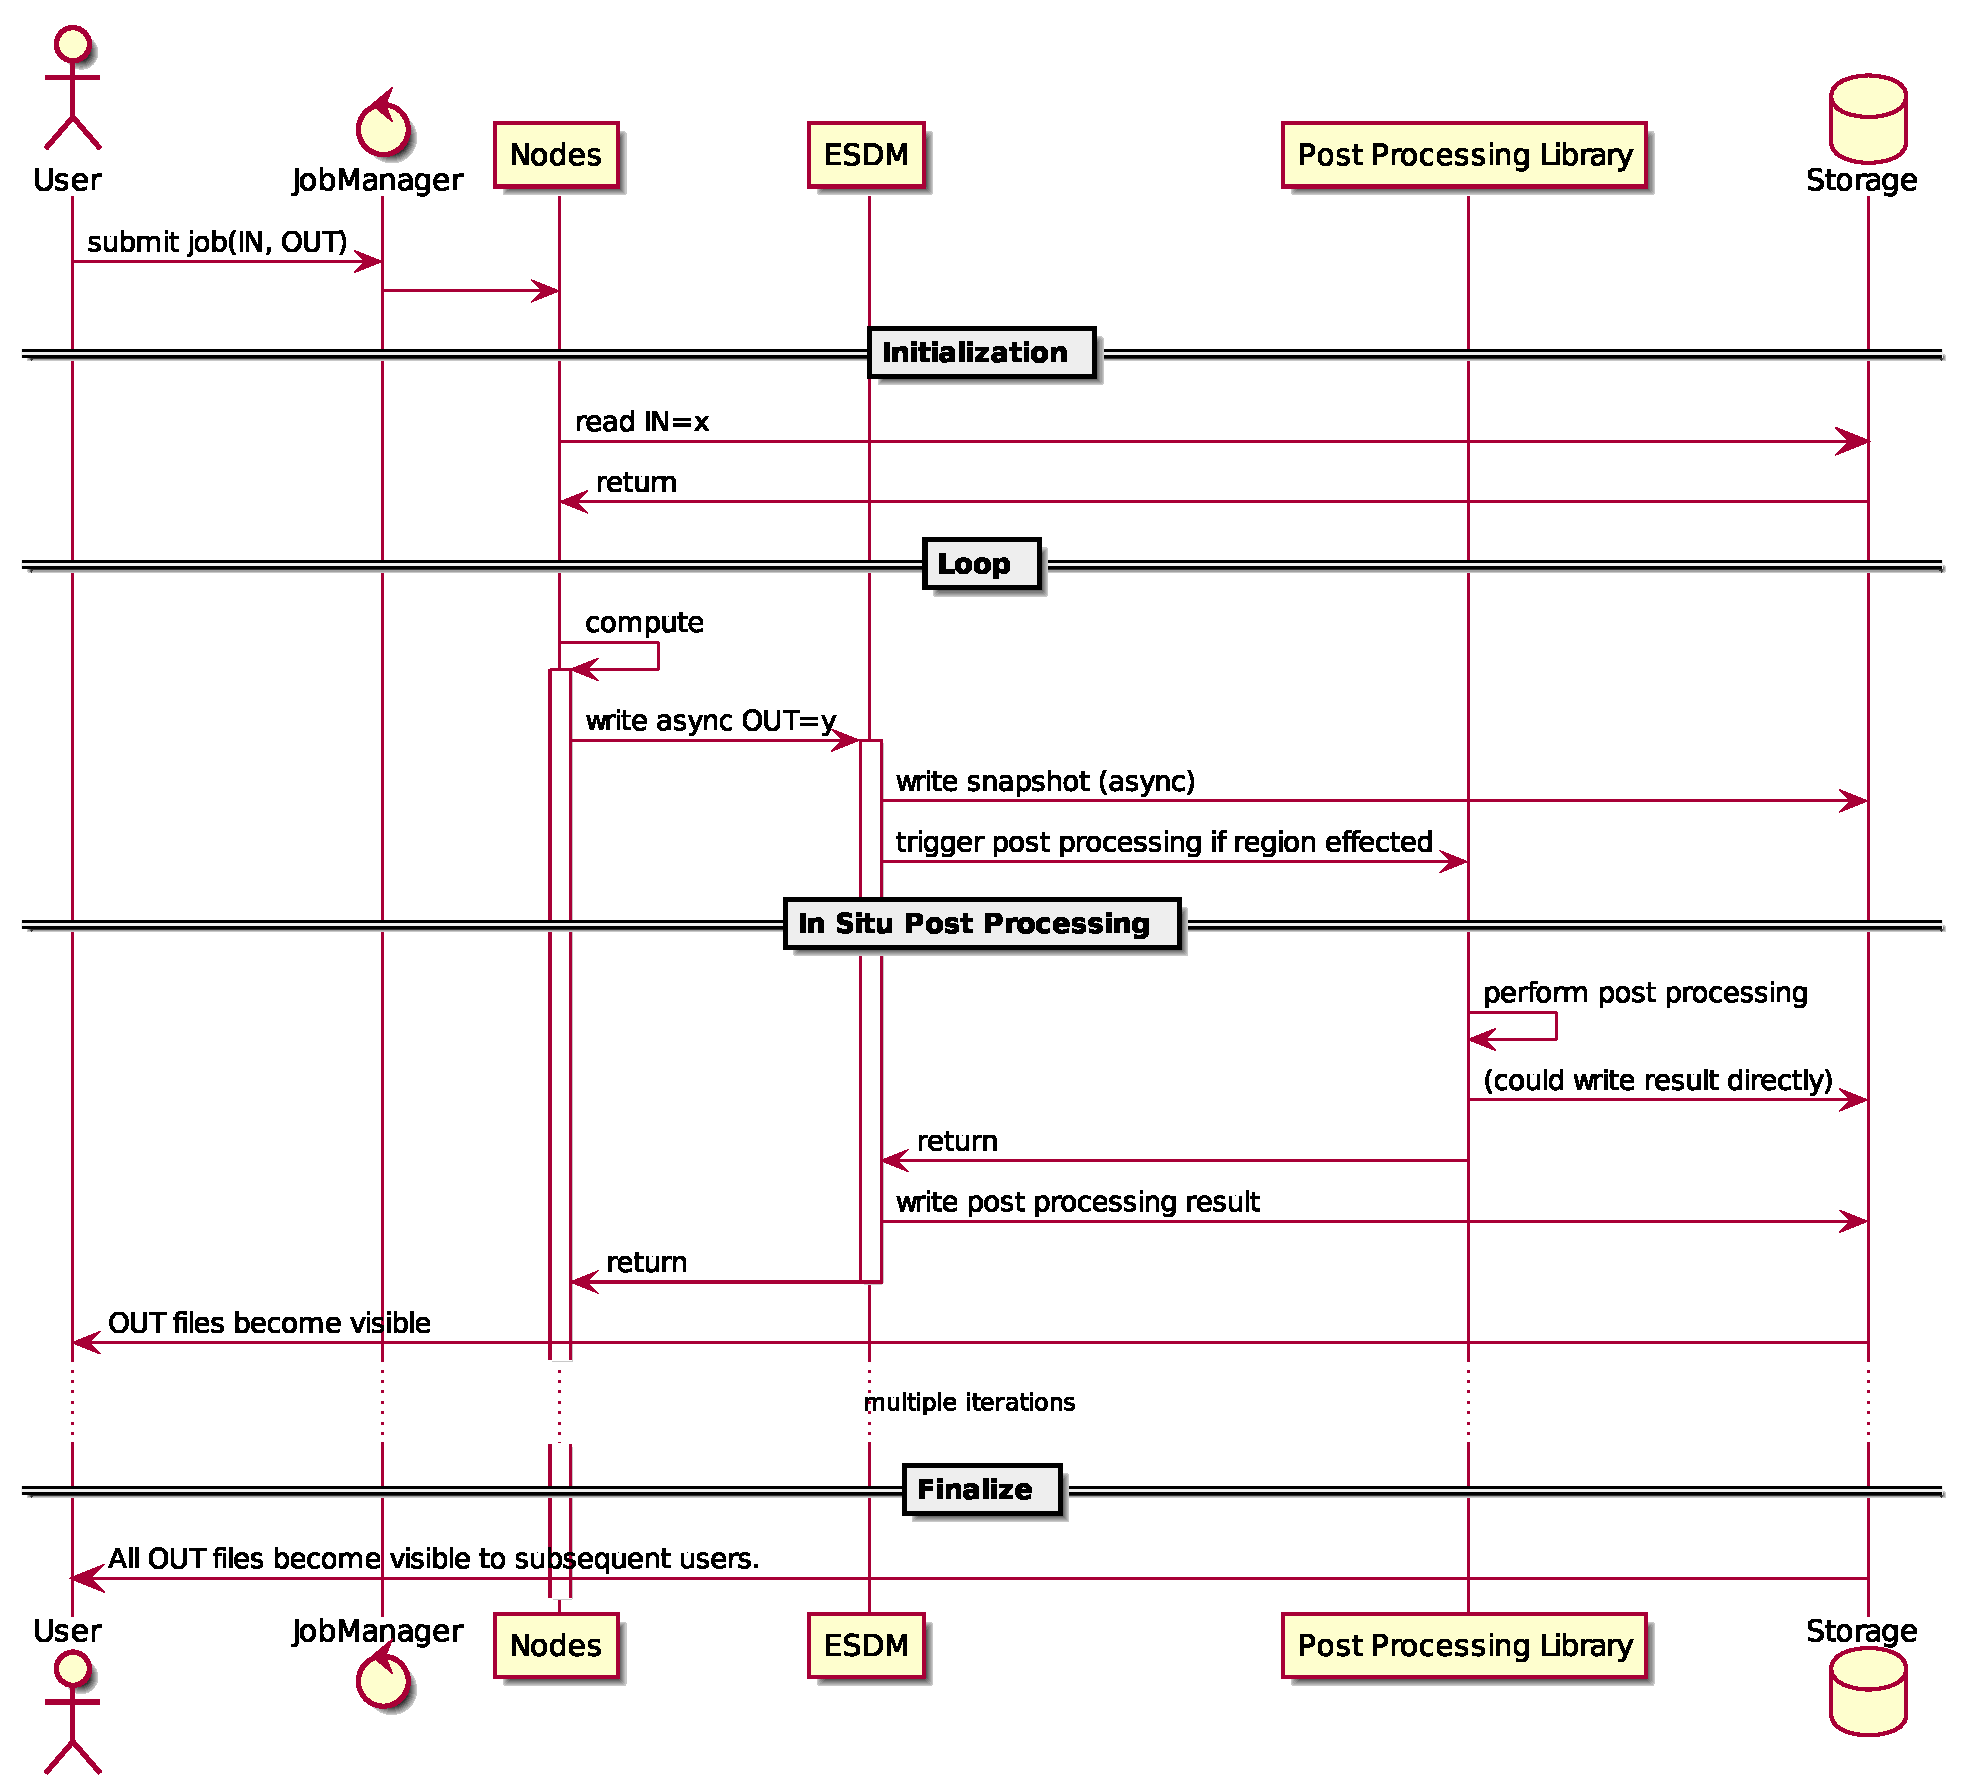
\includegraphics[width=\linewidth]{use-cases/uml/simulation+insitu+postproc/sequence.eps}
	\caption{Sequence Diagram for Simulation + In situ post processing.}
	\label{fig:sequence in-situ}
\end{figure}




\paragraph{Exceptions:}
\begin{enumerate}
	\item Simulation can fail and if snapshots are being written consistency checks need to be performed and unnecessary fragments require clean up (see UC: Simulation \Cref{uc: simulation}).
	\item Post processing could fail
\end{enumerate}


%\paragraph{Subordinate Use-Cases:}
%\begin{itemize}
%	\item For special cases that are not adequate as a scenario. If any.
%\end{itemize}



%%%%%%%%%%%%%%%%%%%%%%%%%%%%%%%%%%%%%%%%%%%%%%%
\subsection{UC: Simulation + In situ + Interactive Visualisation}
\label{uc: simulation + in-situ + cam}


Periodically writing snapshots of the model state typically slows down the simulations considerably, because the simulation has to wait for the I/O systems to finish writing a snapshot before it can continue.
Additional resources such as I/O nodes or burst buffers can be used to flush data asynchronously from the application and, thus, prevents climate applications from waiting for I/O.
An alternative can be to inspect simulations directly by using in-situ visualisation.
\Cref{uc: simulation + big data + in-situ} describes a similar use case that applies big data analytics to detect anomalies before notifying a user for in-situ inspection.


\paragraph{Use-Case Description:}
A job is spawned on multiple nodes which collectively run a simulation of the earth system (see \Cref{uc: simulation}).
As the simulation proceeds a user can render the current state of the simulation using a visualisation tool.
Over time, the user may choose to change the camera view, which variables are included in visualisation.
\Cref{fig:sequence simulation + in-situ + cam} illustrates the sequence of events in more detail.

\paragraph{Priority:}
Low - Not in scope of project to integrate with in-situ frameworks.

\paragraph{Actors:}
\begin{itemize}
	\item Scientist
	\item Application
	\item Supercomputer
	\item Visualisation	Cluster
	\item ESDM
\end{itemize}


\paragraph{Data/Domain Description and Decomposition:}
The logical model domain corresponds to the domain description and decomposition in the UC: Simulation (compare to \Cref{uc: simulation}).
In addition, the camera window requires to be rendered:
Depending on the position of the camera, different compute nodes and visualisation nodes have to communicate (see \Cref{fig:domain simulation + in-situ + cam}).
Each visualisation node is only responsible for defined region of the cameras view (e.g. top left quarter of the domain).


\begin{figure}
	\centering
	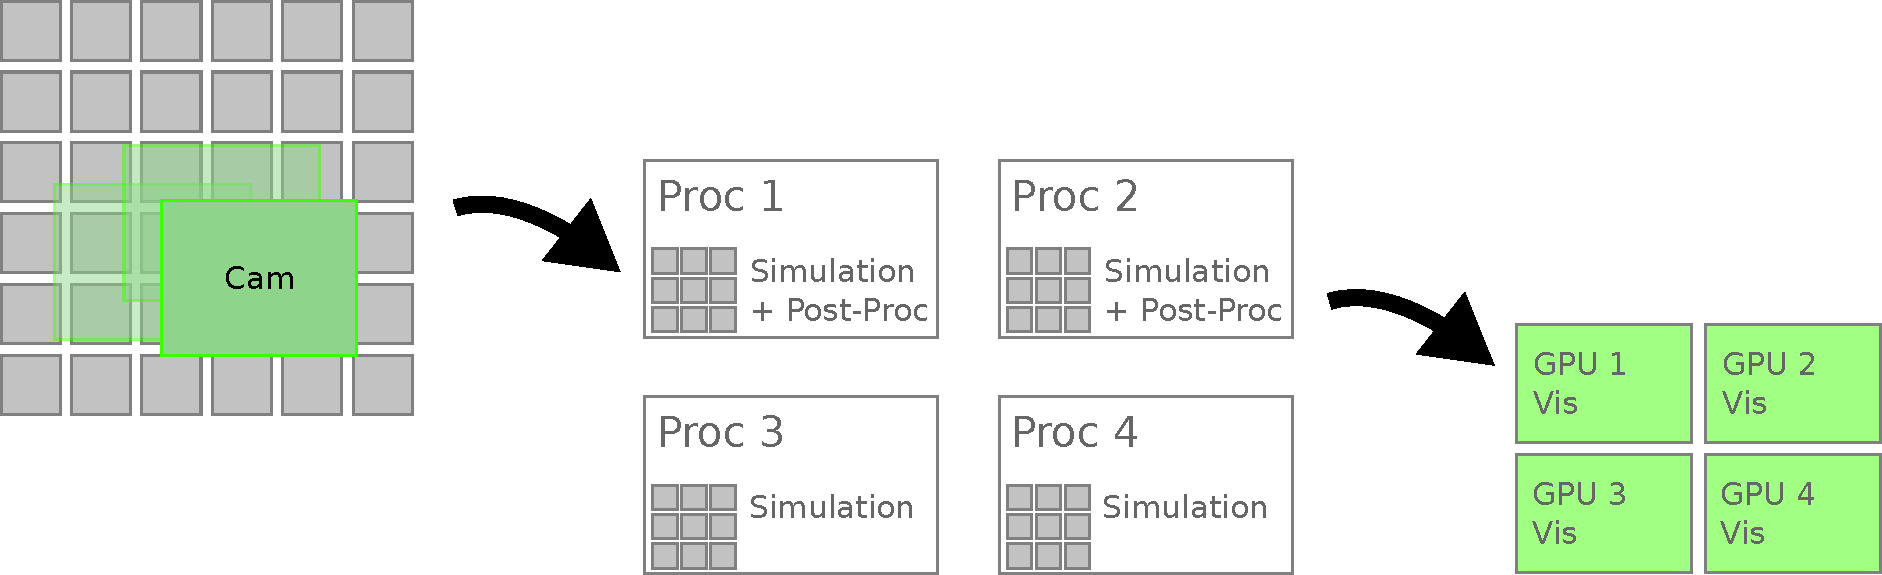
\includegraphics[width=0.5\linewidth]{use-cases/uml/simulation+insitu+camara/domain}
	\caption{Domain Illustration}
	\label{fig:domain simulation + in-situ + cam}
\end{figure}



\paragraph{Pre-Conditions:}
\begin{itemize}
	\item Input and output destinations are accessible to the user.
	\item A allocation to a supercomputer is granted by the resource manager.
	\item A allocation to a visualisation cluster is granted (possibly part of the same super computer).
\end{itemize}


\paragraph{Post-Conditions:}
From an ESDM perspective no post-conditions have to hold because no data is written.
Alternatively, if a user decides to start storing snapshots, the post-conditions of UC: Simulation apply (see \Cref{uc: simulation}).




\paragraph{Related Use-Cases:}
\begin{itemize}
	\item Adapts: Simulation (\Cref{uc: simulation})
\end{itemize}


\paragraph{Flow of Events:}
\begin{enumerate}
	\item Scientist: submits jobs to run on an application with containers for input and output specified. In addition, a list of required post processing is provided (provided by the job script, derived from a workflow or possibly learned automatically).
	\item Workload manager: eventually allocates resources to start job. (ESDM can optimize prior to job start see \Cref{uc: simulation}).
	\item Application opens the IN container (read-only) in collective mode.
	\item ESDM: optimizes the container for read mode (optionally done during staging mode).
	\item Application opens the OUT container (write-only) in collective mode, allocate known space if necessary.
	\item ESDM: prepares the container for write mode.
	\item Application: announces to read initial simulation data.
	\item See UC: Read, it might be collective (better) or independent.
	\item Application: runs the time series of computation:
	\begin{enumerate}
		\item Process: Reads auxiliary data (if necessary), see UC: Read
		\item ESDM: identifies storage devices
		\item Process: Computes (and communicate)
		\item Process: Writes subset of variables
		\item ESDM: receives data and data is only buffered for a limited number of timesteps
		\item ESDM: exchanges data within camera view to visualisation nodes
		\item Visualisation: Renders a frame for current view (as user moves camera rerenders may become necessary if not cached)
	\end{enumerate}
	\item Application: finishes computation and terminates.
	\item Workload Manager: free the resources, manage evtl. stage occupied local storage resources.
\end{enumerate}


\begin{figure}
	\centering
	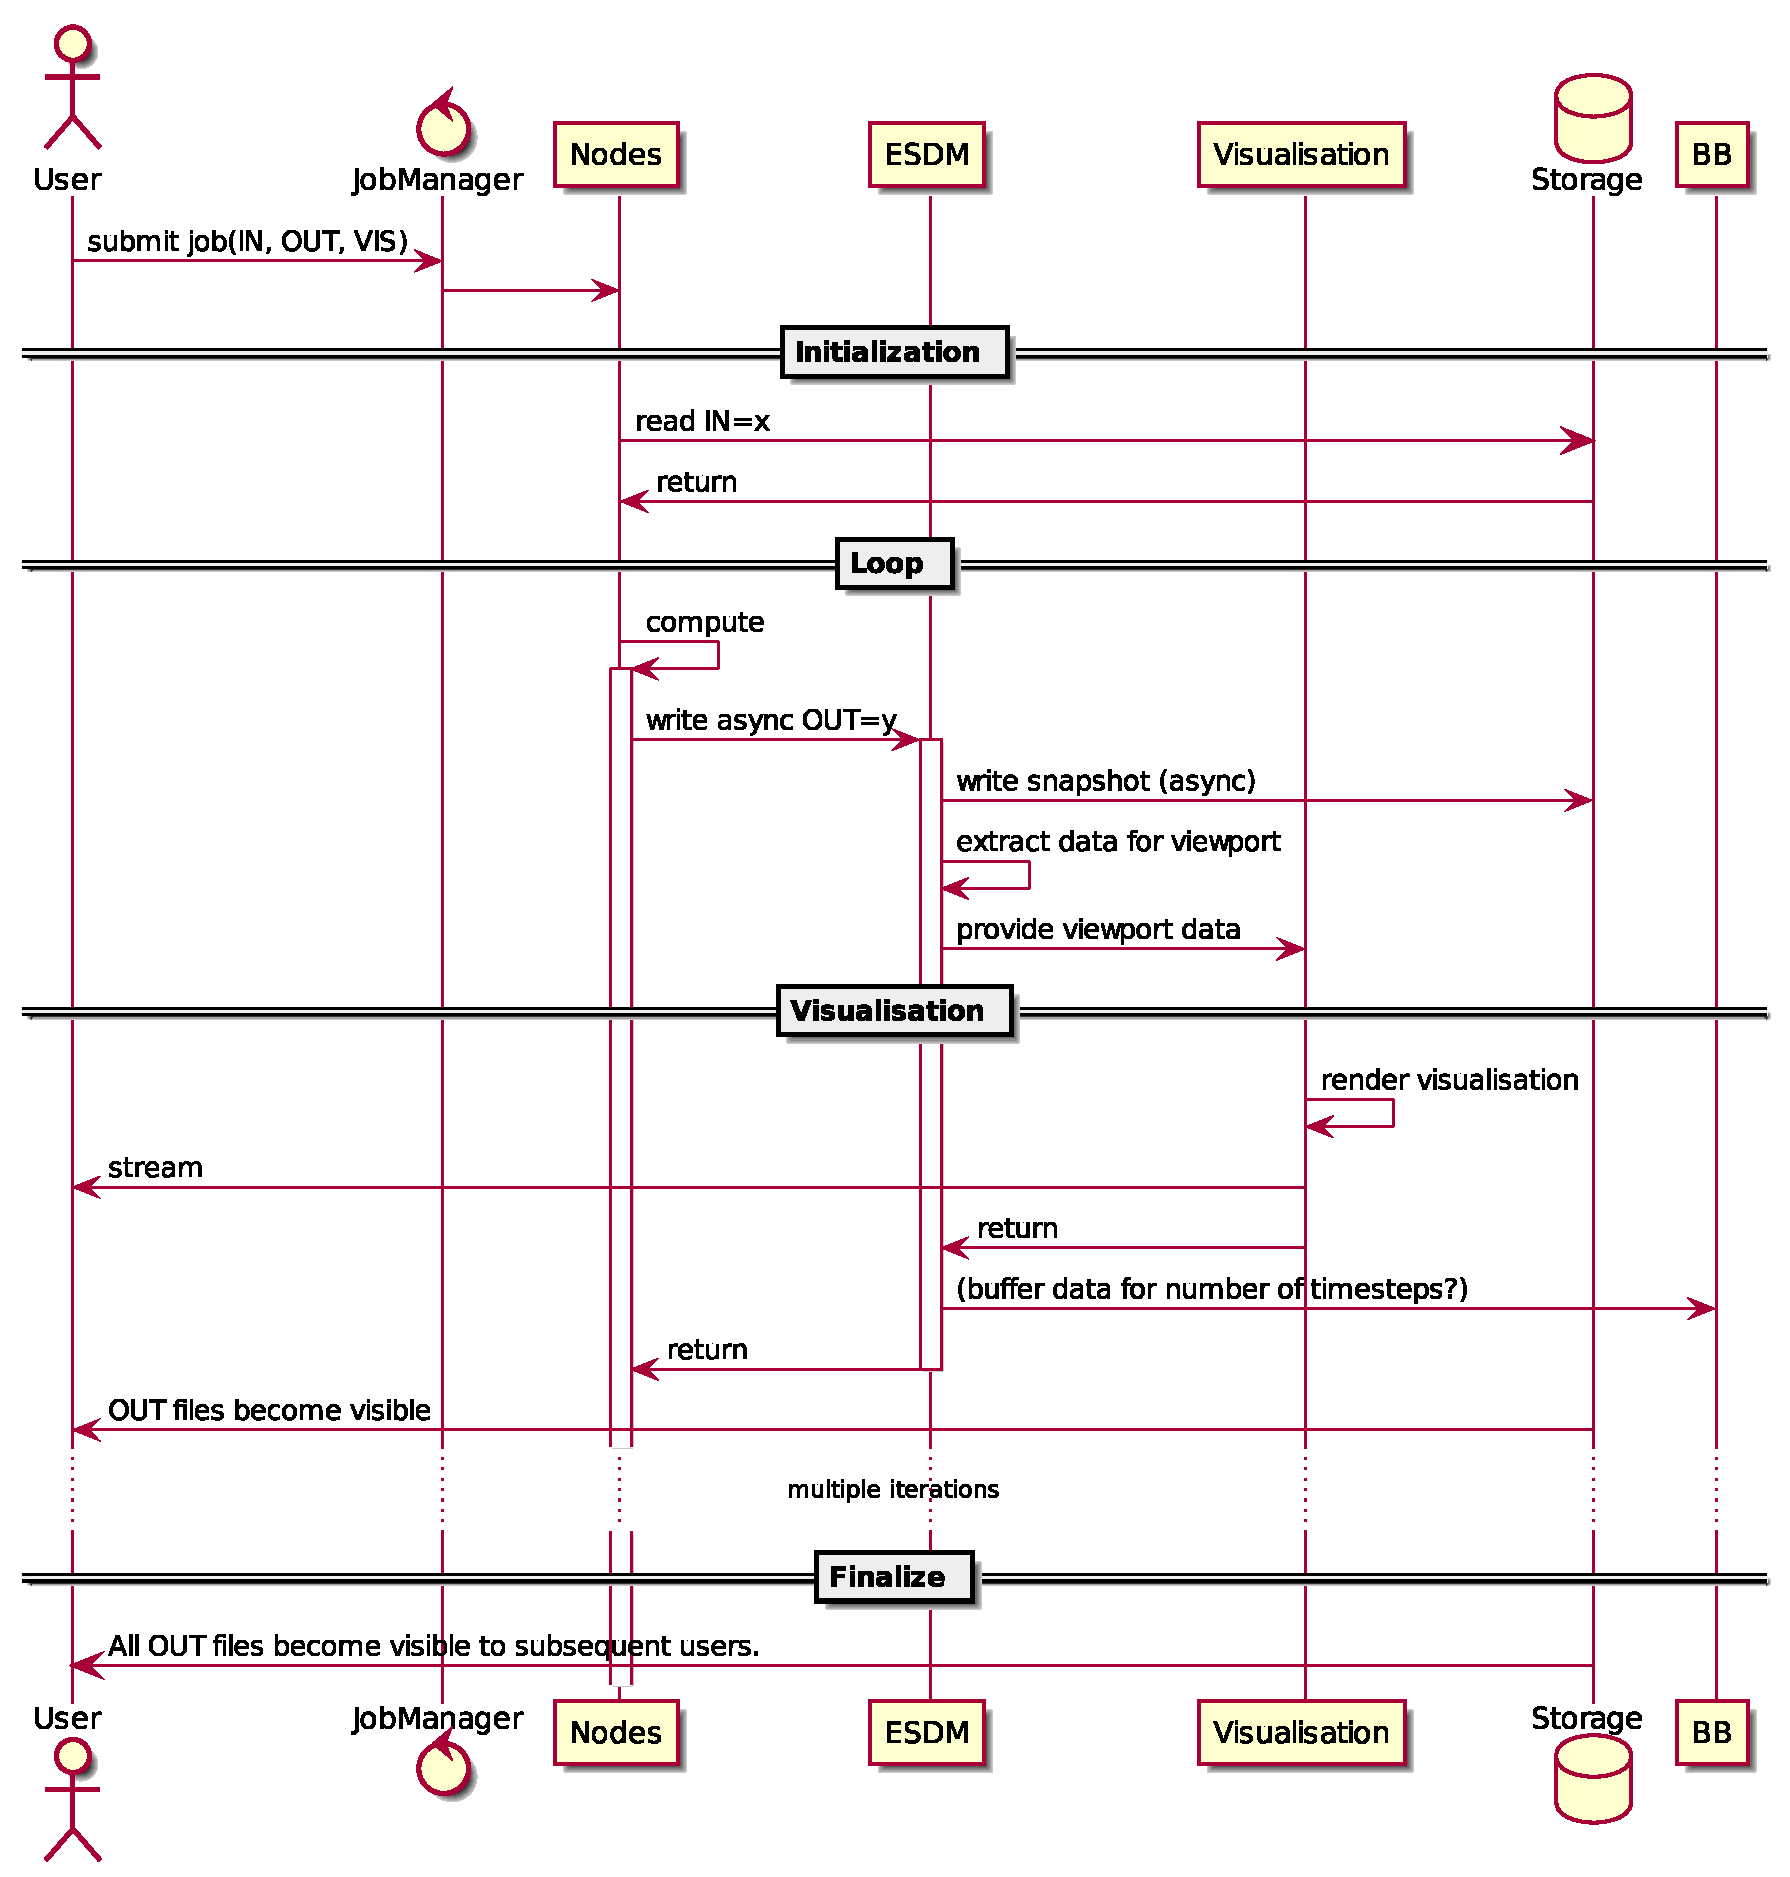
\includegraphics[width=\linewidth]{use-cases/uml/simulation+insitu+camara/sequence.eps}
	\caption{Sequence Diagram}
	\label{fig:sequence simulation + in-situ + cam}
\end{figure}



\paragraph{Exceptions:}
\begin{enumerate}
	\item Simulation can fail and if snapshots are being written consistency checks need to be performed and unnecessary fragments require clean up (see UC: Simulation \Cref{uc: simulation}).
	\item Visualisation cluster may fail. It could be a responsibility of the ESDM to re-spawn the visualisation In terms of data consistency no actions are required by the ESDM.
\end{enumerate}





%%%%%%%%%%%%%%%%%%%%%%%%%%%%%%%%%%%%%%%%%%%%%%%
\subsection{UC: Simulation + Big Data Analysis + In situ analysis/visualisation}
\label{uc: simulation + big data + in-situ}

Inline with the previous in-situ use cases (see \Cref{uc: simulation + in-situ + post processing} and \Cref{uc: simulation + in-situ + cam}), the goal is to take stress off the storage system, in this case by being more selective about which snapshots are permanently stored.
Big data tools in combination with machine learning techniques promise to allow computers to automatically apply complex analysis tasks on large amounts of data.
Such analysis is already applied to satellite data e.g. to track biodiversity, combating desertification or detect wild fires.
In the future, this might be also applied to faux satellite images  generated from model output (or the raw data directly) to better characterize the impact on various ecological factors of climate policy actions.



\paragraph{Use-Case Description:}
A parallel job is started in which multiple nodes collectively simulate the earth system (see \Cref{uc: simulation}).
As the simulation runs, no data is written but using big data analytics anomalies or F of interest is detected.
A configuration defines what actions are triggered.
Additional jobs could be started or a scientist is notified about an anomaly to perform additional analysis jobs or use visualisation.
\Cref{fig:sequence simulation + big data + in-situ} provides a sequence diagram on the flow of events for this use case.

\paragraph{Priority:}
Low - Not in scope of project to integrate with in-situ frameworks and big data cluster systems.

\paragraph{Actors:}
\begin{itemize}
	\item Scientist
	\item Application
	\item Supercomputer
	\item Big Data Analysis Cluster (this could also be the supercomputer)
	\item ESDM
	\item Pre/Post Processing Framework
\end{itemize}


\paragraph{Data/Domain Description and Decomposition:}
Multiple domain decompositions are at play in this use case.
The simulation decomposition corresponds to the description in UC: Simulation (\Cref{uc: simulation}) except that we assume no snapshots are permanently stored until a trigger condition occurs.
The big data analysis workloads do not follow a fixed structure and heavily depend on the analysis performed.
UC: Pre/Post Processing (see \Cref{uc: pre + post processing}) illustrated multiple possible access patterns which also apply here.
More sophisticated analysis may be also responsive to the time evolution within a simulation, for example a storm might move within the simulation, the analysis could follow the storm in which case a situation similar to UC: Simulation + Interactive in-situ visualisation (compare to {uc: simulation + in-situ + cam}) is more appropriate.


%\begin{figure}
%	\centering
%	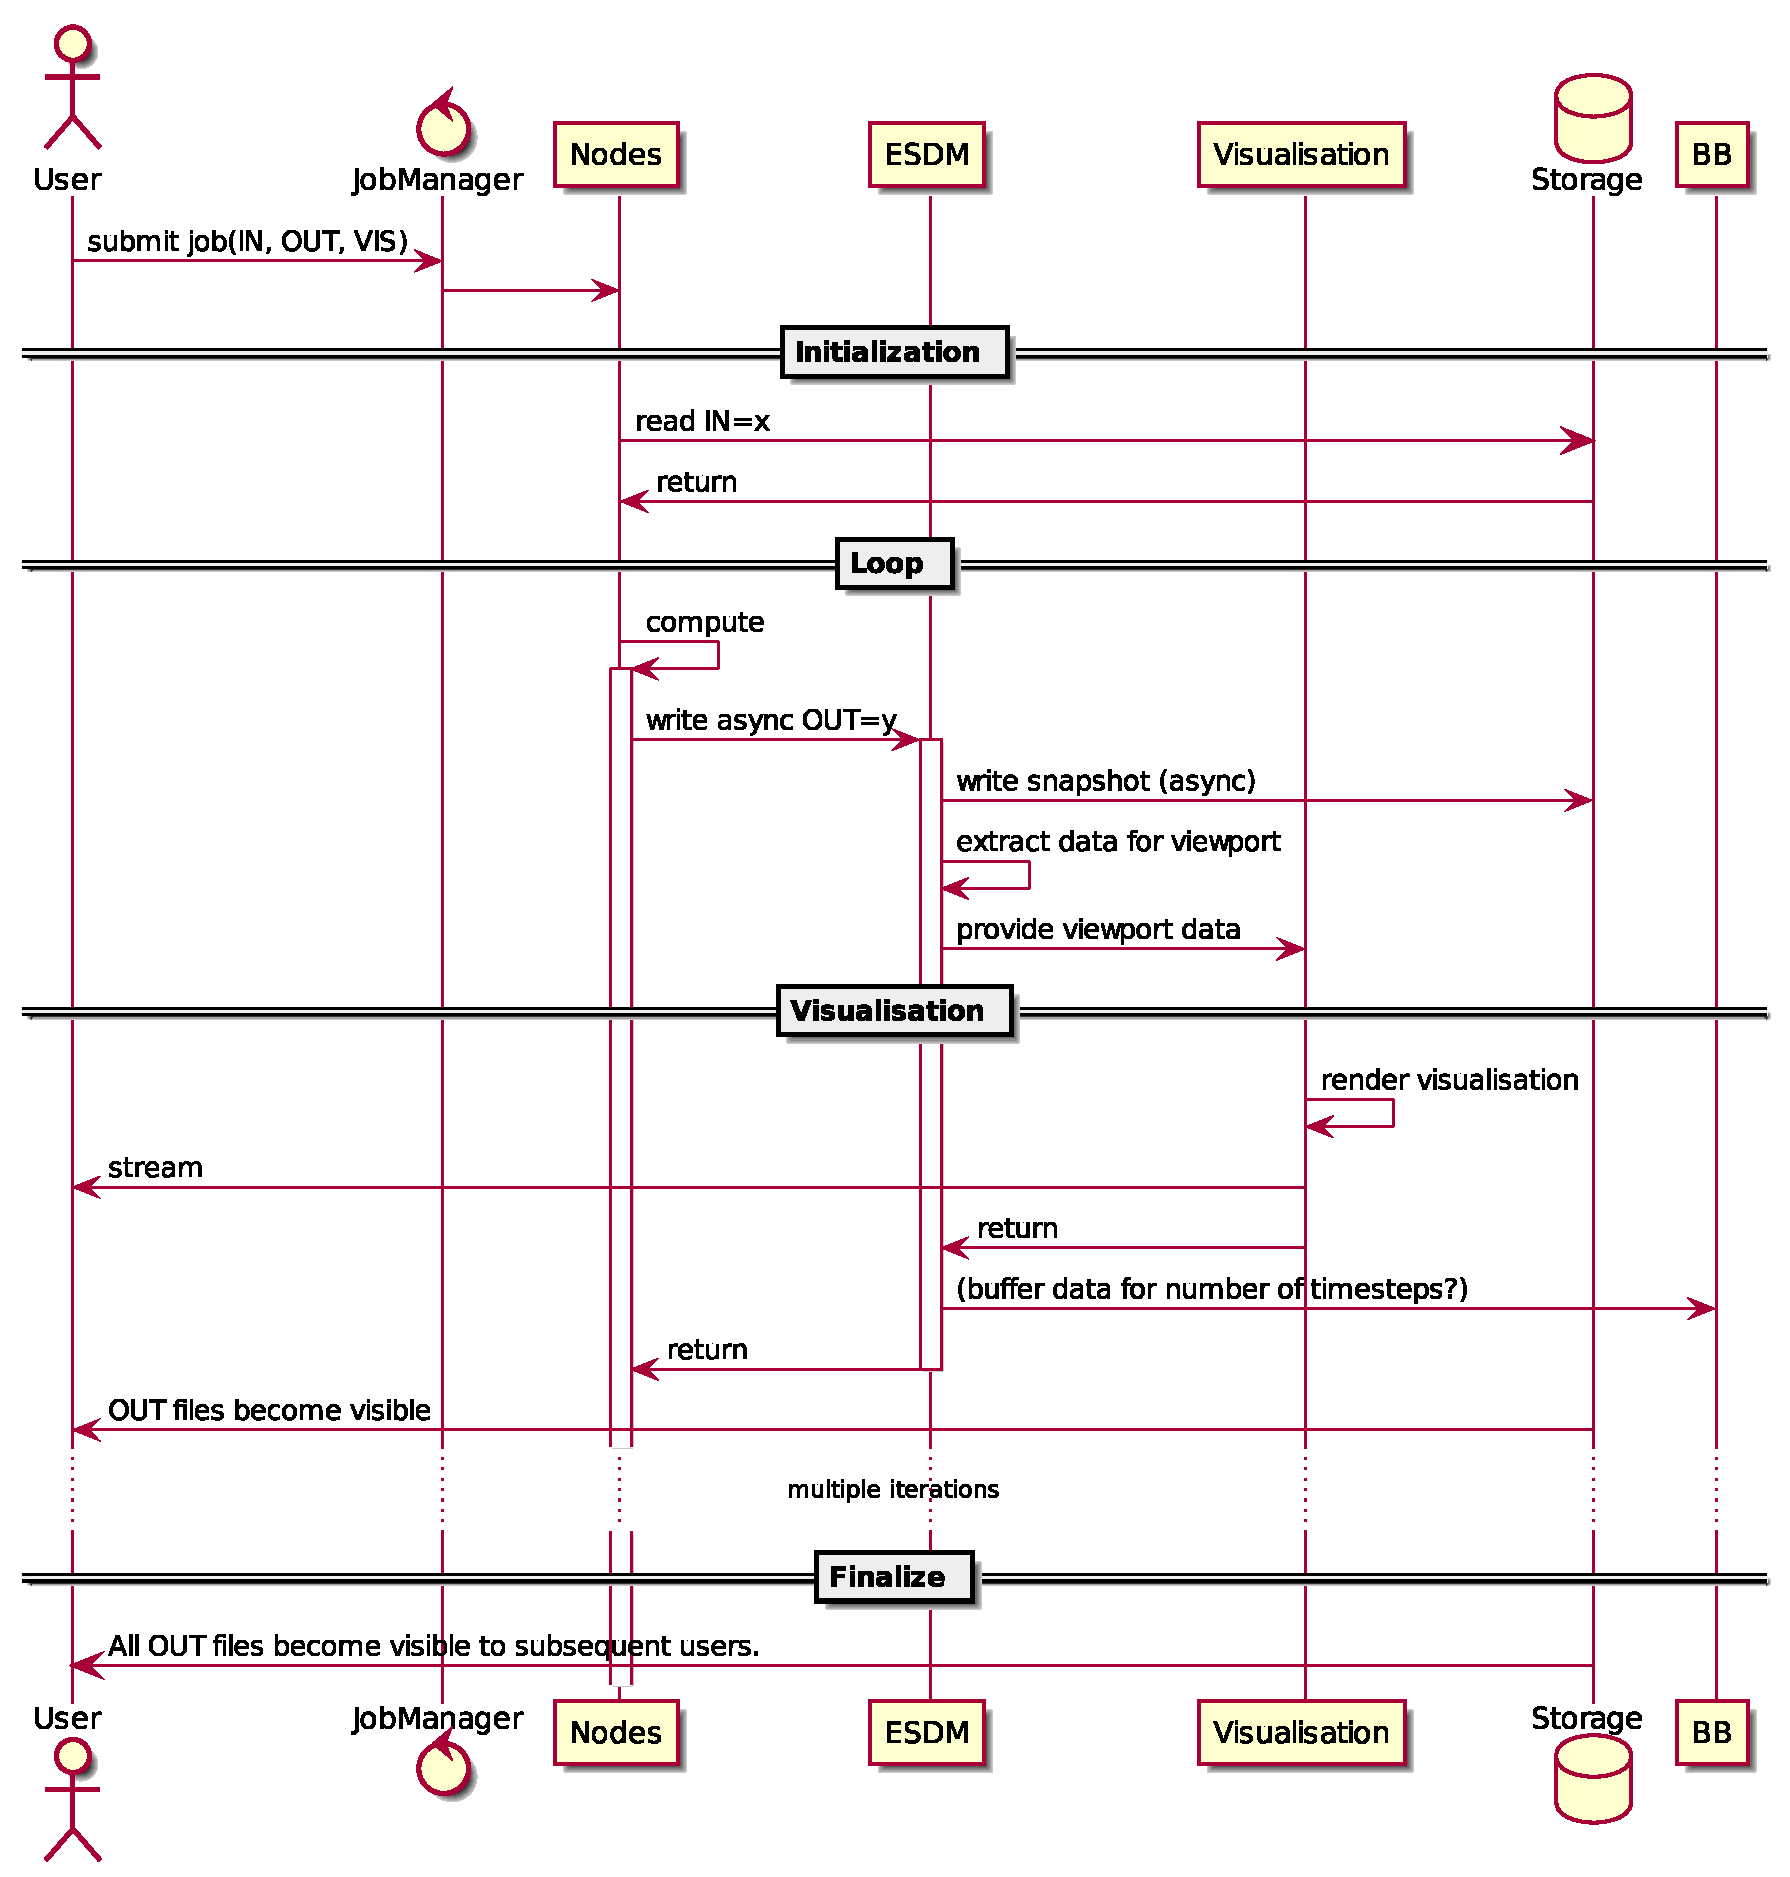
\includegraphics[width=\linewidth]{use-cases/uml/simulation+insitu+camara/sequence.eps}
%	\caption{Sequence Diagram}
%	\label{fig:sequence simulation + big data + in-situ}
%\end{figure}


\paragraph{Pre-Conditions:}
\begin{itemize}
	\item Pre-conditions as with UC: Simulation
	\item User has nodes allocated for Big Data Analysis
	\item Available resources to add jobs as required for per-processing
\end{itemize}

\paragraph{Post-Conditions:}
\begin{itemize}
	\item Data that users wants to preserve is permanently stored
\end{itemize}




\paragraph{Flow of Events:}
\begin{enumerate}
	\item Scientist: submits a jobs to run an application with containers for input and output specified. In addition, a list of required post processing is provided (provided by the job script, derived from a workflow or possibly learned automatically).
	\item Workload manager: eventually allocates resources to start job. (ESDM can optimize prior to job start see \Cref{uc: simulation}).
	\item Application opens the IN container (read-only) in collective mode.
	\item ESDM: optimizes the container for read mode (optionally done during staging mode).
	\item Application opens the OUT container (write-only) in collective mode, allocate known space if necessary.
	\item ESDM: prepares the container for write mode.
	\item Application: announces to read initial simulation data.
	\item See UC: Read, it might be collective (better) or independent.
	\item Application: runs the time series of computation:
	\begin{enumerate}
		\item Process: Read auxiliary data (if necessary), see UC: Read
		\item ESDM: identifies storage devices
		\item Process: Computes (and communicate)
		\item Process: Writes subset of variables
		\item ESDM: receives data but no permanent data is stored yet
		\item ESDM: makes data available to big data analysis cluster (e.g. burst buffer)
		\item Big Data Cluster: performs analysis (this may take a while)
		\item ESDM: eventually analysis receives result. If trigger condition matches:
		\begin{enumerate}
			\item ESDM: may notify the user
			\item ESDM: may start to write snapshots
			\item ESDM: may invoke callback/run script
		\end{enumerate}
	\end{enumerate}
	\item Application: closes the container.
	\item Application: finishes computation and terminates.
	\item Workload Manager: free the resources, manage evtl. stage occupied local storage resources.
\end{enumerate}



\begin{figure}
	\centering
	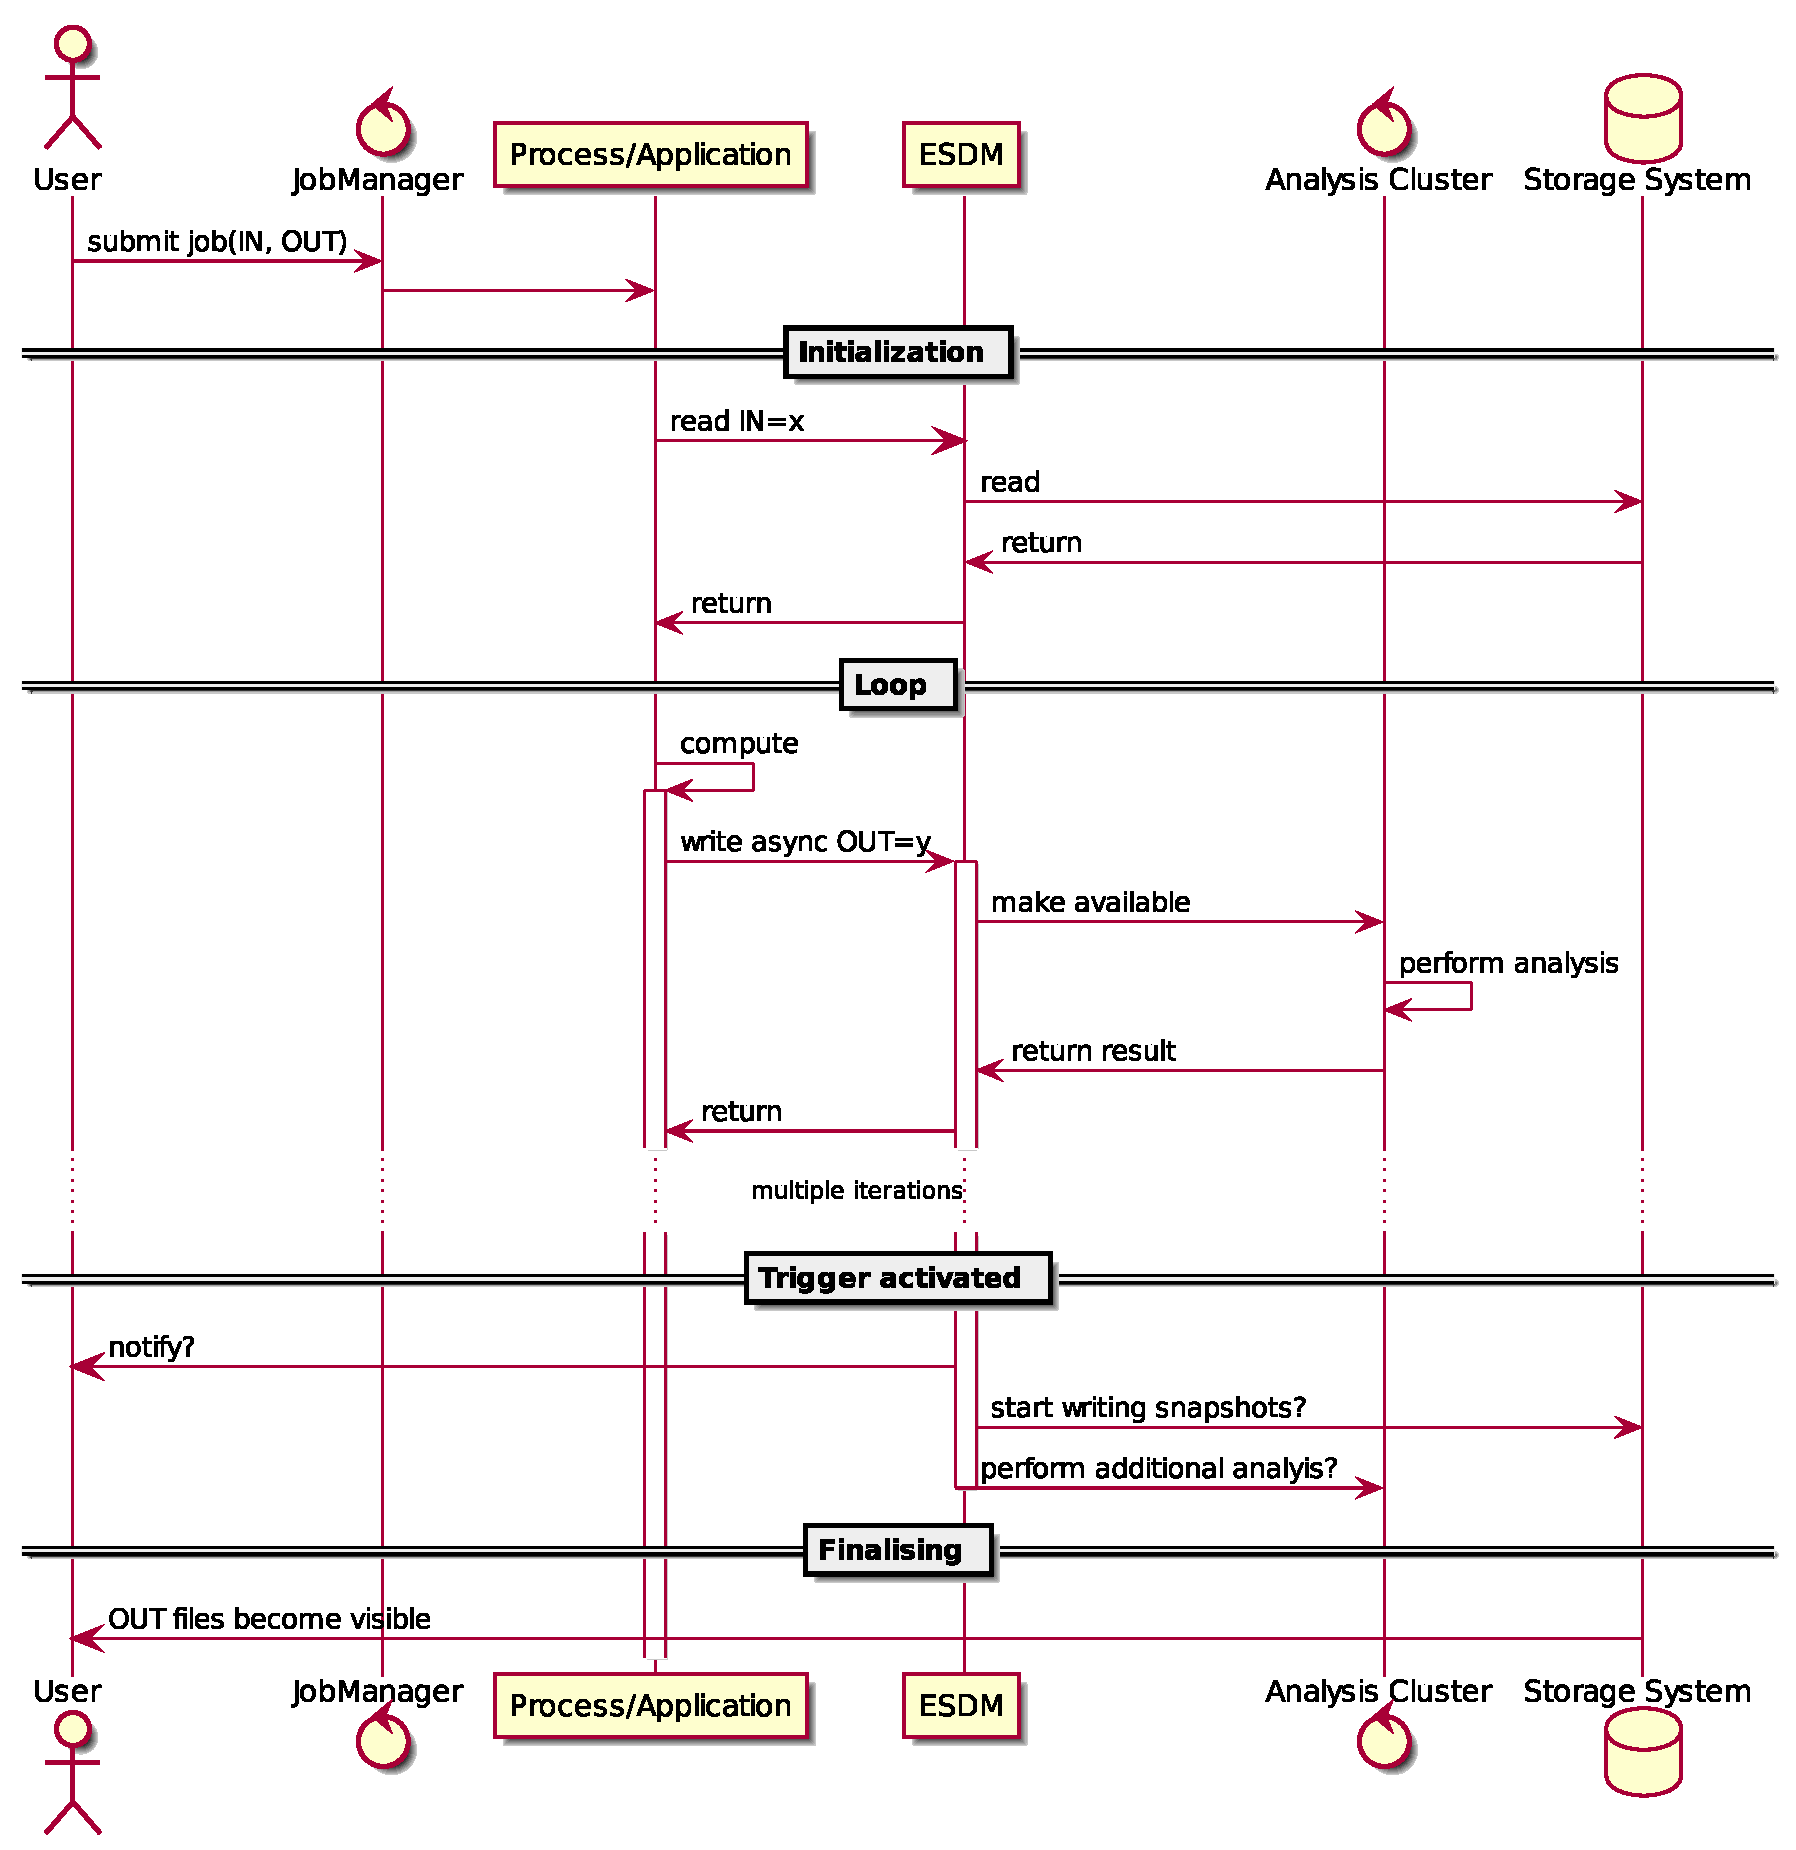
\includegraphics[width=\linewidth]{use-cases/uml/simulation+insitu+bigdata/sequence.eps}
	\caption{Sequence Diagram}
	\label{fig:sequence simulation + big data + in-situ}
\end{figure}



\paragraph{Related Use-Cases:}
\begin{itemize}
	\item Adapts: Simulation (\Cref{uc: simulation})
	\item Adapts: Pre/Post Processing on existing data (\Cref{uc: pre + post processing})
\end{itemize}






\paragraph{Exceptions:}
\begin{enumerate}
	\item Simulation can fail and if snapshots are being written consistency checks need to be performed and unnecessary fragments require clean up (see UC: Simulation \Cref{uc: simulation}).
	\item Big data cluster may fail. It could be a responsibility of an ESDM to resubmit tasks for analysis.
\end{enumerate}




%%%%%%%%%%%%%%%%%%%%%%%%%%%%%%%%%%%%%%%%%%%%%%%%%%%%%%%%%%%%%%%%%%%%%%%%%%%%%%%
\chapter{Architecture: Viewpoints}
\label{chap:viewpoints}
\begin{chapterIntro}
This section introduces a high-level overview for the earth system middleware (ESDM) and discusses the architecture according to the 4+1 model (refer to \Cref{sec:about 4+1}).
\Cref{sec: viewpoints/logical} starts with an architecture overview and introduces the core components and their relation to wide spread technologies related to I/O in earth system software.
\Cref{sec: viewpoints/logical} covers the logical view, i.e, multiple aspects that affect how the ESDM operates and which semantics apply internally as well as externally to users/software using the ESDM.
In particular, this includes the responsibilities of key components, the underlying data model and operations to manipulate the data including a mechanism to manage epochs.
In \Cref{sec: viewpoints/physical}, the components are related to their physical location within the hardware and software stacks.
\Cref{sec: viewpoints/process}, discusses active components and processes required by the ESDM and how they interact when working concurrently.
%\Cref{sec: viewpoints/development}, provides the development view and names required interfaces and how to represent information about and within the data model.
\end{chapterIntro}


%%%%%%%%%%%%%%%%%%%%%%%%%%%%%%%%%%%%%%%%%%%%%
\section{Logical View: Component Overview}
\label{sec: viewpoints/logical}


The architecture overview provides only a brief description of the core components of the ESDM.
We will refine the preliminary description of this document while we are building the prototype.
While this document provides an overview of the ultimate system, within the ESiWACE project we will only be able to build a prototype for the central pieces.
We seek to demonstrate the benefit of the middleware for the community to sustain development towards the presented vision.
For more detailed descriptions in particular for the backends refer to \Cref{chap:components and backends}.


%%%%%%%%%%%%%%%%%%%%%%%%%%%%%%%%%%%%%%%%%%%%%%%%%%%%%%%%%%%%%%%%%%%%%%%%%%%%%%%
\paragraph {Problem Summary}
The ESD middleware has been designed to deal with the fact that existing  data
libraries for standardised data description and optimised I/O such as NetCDF,
HDF5 and GRIB do not have suitable performance portable optimisations which
reflect current data intensive system architectures and deliver cost-effective,
acceptable data access bandwidth, latency and data durability.

%%%%%%%%%%%%%%%%%%%%%%%%%%%%%%%%%%%%%%%%%%%%%%%%%%%%%%%%%%%%%%%%%%%%%%%%%%%%%%%
\paragraph {The ESD Middleware}
To address these issues of performance portability, and exploiting exiting shared, interoperable interfaces, based on open standards, we have designed the \textit{Earth System Data (ESD)} middleware (ESDM in short), which:
\begin{enumerate}
	\item understands application data structures and scientific metadata, which lets us expose the same data via different APIs;
	\item maps data structures to storage backends with different performance characteristics based on site specific configuration informed by a performance model;
	\item yields best write performance via optimised data layout schemes that utilise elements from log-structured file systems;
	\item provides relaxed access semantics, tailored to scientific data generation for independent writes, and;
	\item includes a FUSE module which will provide backwards compatibility through existing file formats with a configurable namespace based on scientific metadata.
\end{enumerate}

Together these allow storing small and frequently accessed data on node-local storage, while serialising multi-dimensional data onto multiple storage backends -- providing fault-tolerance and performance benefits for various access patterns at the same time.
Compact-on-read instead of garbage collection will additionally optimise and replicate the data layout during reads via a background service.
Additional tools allow data import/export for exchange between sites and external archives.

The ESDM aids the interests of stakeholders: developers have less burden to provide system specific optimisations and can access their data in various ways.
Data centres can utilise storage of different characteristics.

\bigskip


\begin{figure}[bp]
	\centering
	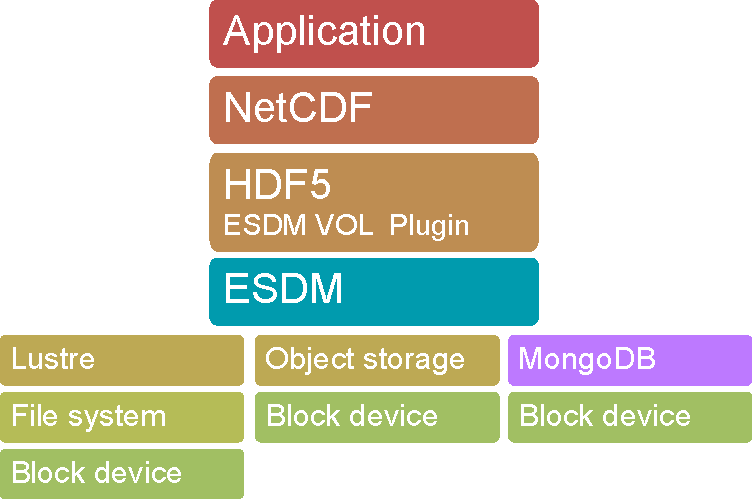
\includegraphics[width=0.5\columnwidth]{figures/layers-esdm}
	\caption{A typical I/O-stack with the ESD middleware}
	\label{fig:architecture-esd-layering}
\end{figure}

\begin{figure}[bp]
	\centering
	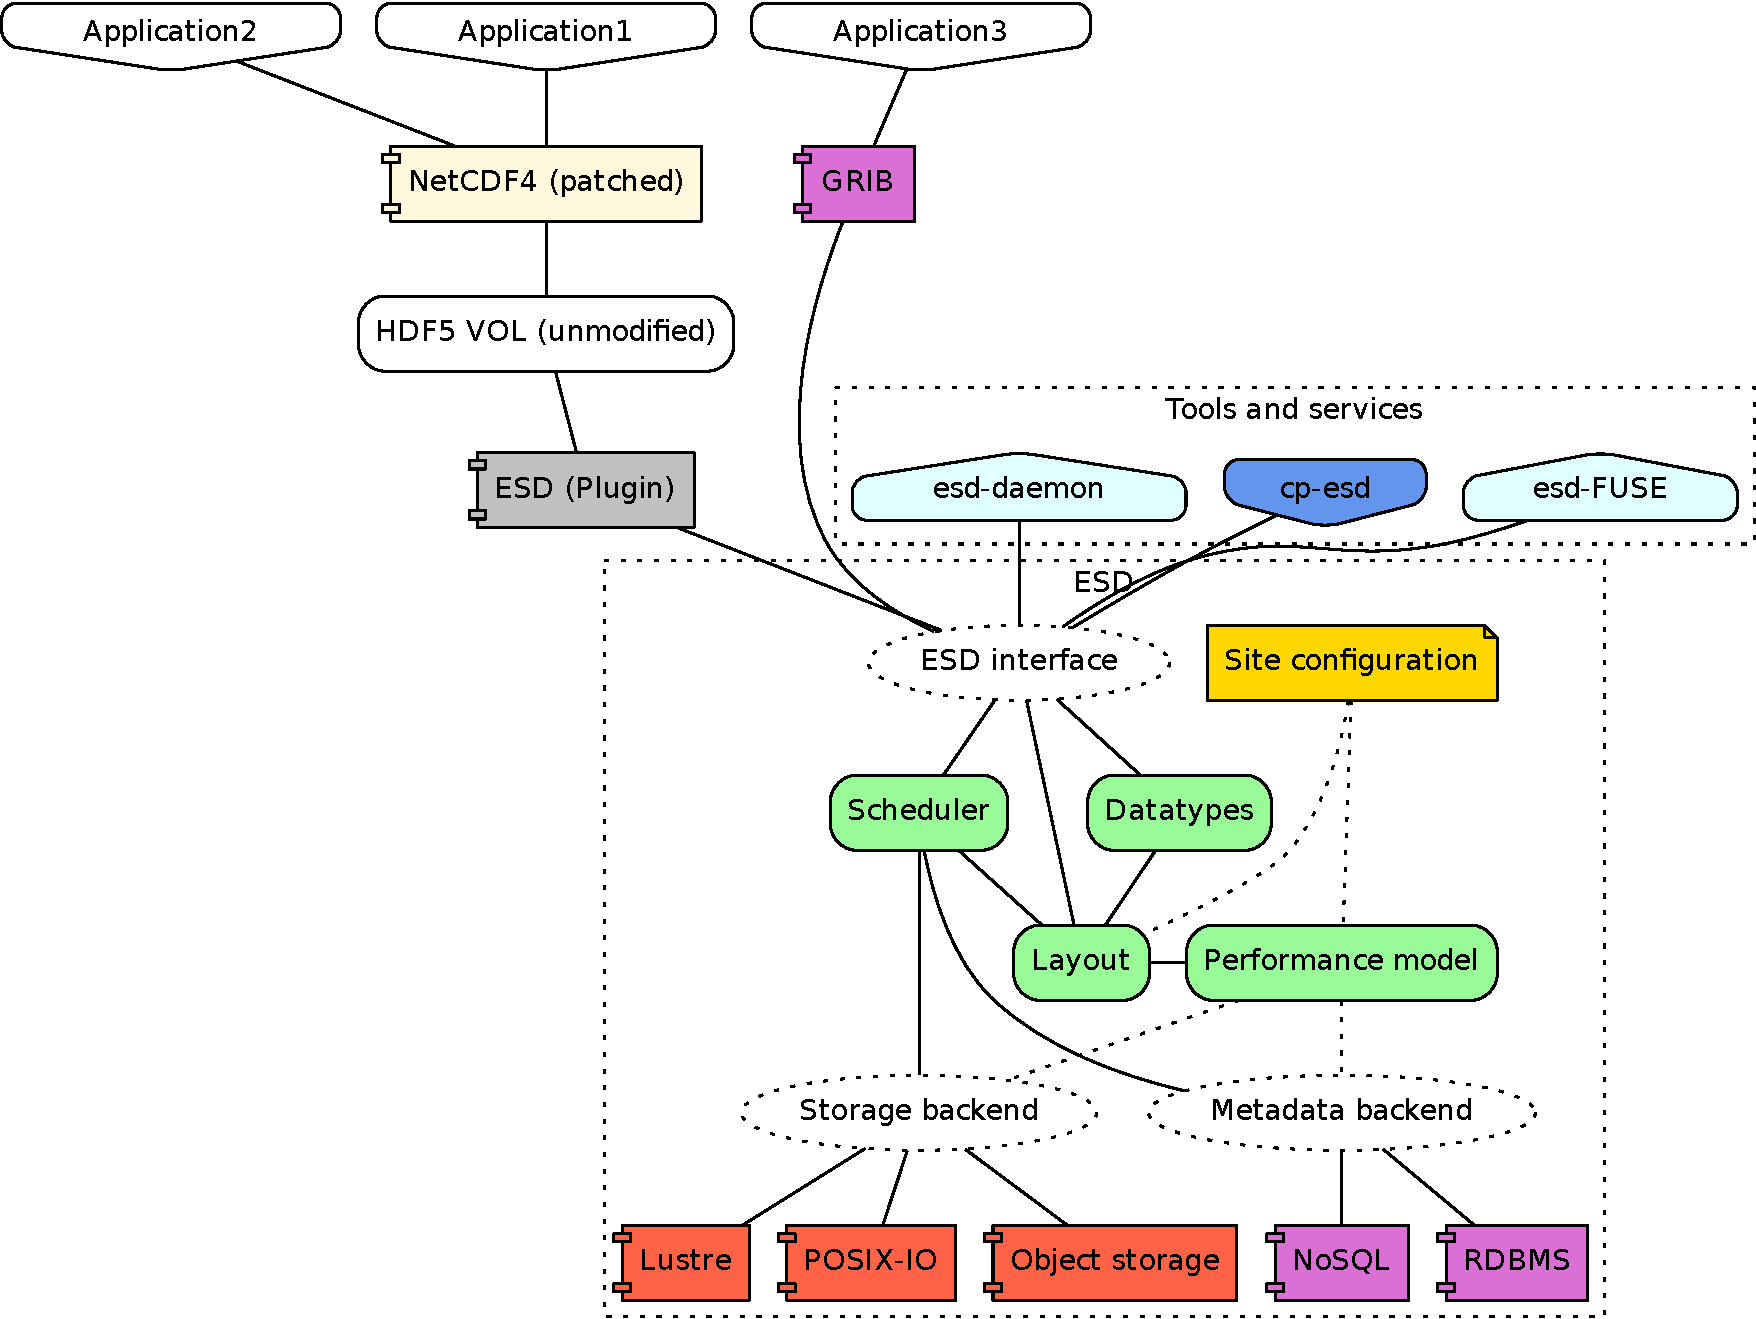
\includegraphics[width=0.98\columnwidth]{architecture-backend_with-scheduler/architecture-backend-src.pdf}
	\caption{Overview of the ESD architecture, relevant components and relationship to application and storage systems.}
	\label{fig:architecture}
\end{figure}

A typical I/O-stack for an application using ESDM is shown in \Cref{fig:architecture-esd-layering}.
I/O of an existing application using the NetCDF (or HDF5) interface is processed by the ESDM plugin of HDF5 which may decide to store data on one of the available
storage backends such as Lustre or an Object storage.
Metadata may be stored in one of the supported metadata plugins.
The user does not have to make decisions regarding the storage or metadata backends to be used; this decision is made by the middleware.

\bigskip


Details of the ESDM architecture is given in \Cref{fig:architecture}.
It provides more details about how ESDM is embedded into the existing software landscape and its high-level components:

\paragraph{Applications}
Use existing storage interfaces such as NetCDF4, GRIB or they may use the ESD interface.

\paragraph{Job scheduler}
The job scheduler assigns supercomputer resources to jobs.
It may use the ESD interface to inform about future activity and stage/unstage data.


\paragraph{Middleware libraries} are adjusted to be layered on top of the ESD interface.


%%%%%%%%%%%%%%%%%%%%%%%%%%%%%%%%%%%%%%%%%%%%%%%%%%%%%%%%%%%%%%%%%%%%%%%%%%%%%%%
\paragraph{ESD Interface}
This represents the API exposed to other libraries and users.
The API is independent of the specific I/O backend used to store the data and supports structured queries to perform complex data selections in the variables.
The API is able to support the complex workflows of future applications.

%%%%%%%%%%%%%%%%%%%%%%%%%%%%%%%%%%%%%%%%%%%%%%%%%%%%%%%%%%%%%%%%%%%%%%%%%%%%%%%
\paragraph{Data Types}
The datatype component provides native data types that can be used by users or other libraries to describe data points inside variables.
We follow the approach pursued by the MPI and HDF5 libraries, that is, we provide a set of native data types and a basic set of datatype constructors that can be used to build custom derived datatypes.

%%%%%%%%%%%%%%%%%%%%%%%%%%%%%%%%%%%%%%%%%%%%%%%%%%%%%%%%%%%%%%%%%%%%%%%%%%%%%%%
\paragraph{Layout}
The layout component allows the middleware to store pieces of data on different backends depending on specific site configuration contained in the performance model.
The layout component in this case takes responsibility for generating additional technical metadata describing data placement and for storing it in the appropriate metadata backend (i.e. MongoDB).
A more detailed description of what technical metadata is, is given in the rest of this section.

\paragraph{Performance model}
This model predicts performance for data access using a site-specific configuration that describes the characteristics of available hardware technology.
It is used by the layout component to make decisions of the data placement.

\paragraph{Scheduler}
The scheduler queues asynchronous calls from the API and processes them.
It dispatches calls to storage and metadata backends and uses the layout component to identify beneficial placement of data.

\paragraph{Metadata backend}
Responsible to store all technical and scientific relevant metadata providing efficient access and manipulation.

\paragraph{Storage backend}
These backends are responsible to transform ESD objects and data structures to storage-technology-specific representations.


\paragraph{Tools and services}
On top of ESDM several user space tools are provided, a few examples are:
The FUSE client provides backwards POSIX compatibility with existing applications.
The daemon checks the consistency and integrity of the data managed by ESDM, potentially triggering actions to clean up and replicate data.
The copy tool allows importing and exporting data from ESD to an existing storage infrastructure.
It also serves as blue-print to embed its capabilities into higher-level tools such as GridFTP.



%%%%%%%%%%%%%%%%%%%%%%%%%%%%%%%%%%%%%%%%%%%%%
%\subsection{Component Responsibilities}
%\label{sec: viewpoints/logical/responsibilities}


%%%%%%%%%%%%%%%%%%%%%%%%%%%%%%%%%%%%%%%%%%%%%%%%%%%%%%%%%%%%%%%%%%%%%%%%%%%%%%%%%%%%%%%%%%
\section{Logical View: Data Model}
\label{sec: viewpoints/logical/data model}


While data types introduced by computer architectures and software libraries are important for the data model, they are discussed separately in \Cref{sec: viewpoints/logical/datatypes}.



The data model of a system organises elements of data, standardises how they represent data entities and how users can interact with the data.
The model can be split into three layers:
\begin{enumerate}
	\item The \textbf{conceptual data model} describes the entities and the semantics of the domain that are represented by the data model and the typical operations to manipulate the data.
	In our case, the scientific domain is NWP/climate.
	\item The \textbf{logical data model} describes the abstraction level provided by the system, how domain entities are mapped to objects provided by the system\footnote{A entity of the domain model such as a car could be mapped to one or several objects.}, and the supported operations to access and manipulate these objects are defined.
	Importantly, the \textbf{logical data model} defines the semantics when using the operations to access and manipulate the system objects.
	For example, a system object of a relational model is a table -- representing attributes of a set of objects -- and a row of a table representing attributes of a single object.
	\item The physical data model describes how the logical entities are finally mapped to objects/files/regions on available hardware.
	The physical data model is partly covered by the backends of ESDM, therefore, the descriptions will stop at that abstraction level.
\end{enumerate}

\subsection{Conceptual Data Model}
\label{subsec: conceptual data model}

Our conceptual data model is aligned with the needs of domain scientists from climate and weather. It reuses and extends from concepts introduced in a data model proposed for the Climate and Forecasting conventions for NetCDF data\footnote {\url{``A CF Data Model and Implementation'', Hassel et al, 2017, GMD submitted}}.

\paragraph{Motivation from climate}



The ESDM needs to store, identify and manipulate data variables,  $V$, containing scientific data from the (continuous) real or model world, discretised within a ``sampling'' domain $d$, that is
\[V=V(d)\]
where $V$ may be air temperature, for instance. The domain $d$ describes the location for each value of $V$, and is a function of its independent dimensions, for instance
\[d = d(Z(z), Y(y), X(x)))\]
where $d$ is a three-dimensional domain described by axes of height, latitude, and longitude, sampled at coordinates found from the complete set of samples $Z(z),Y(y),X(x)$.
Each set of coordinates $x,y,z$  together specifies a location in the atmosphere at which $V$ is specified.



The full dimensionality of the variable may exceed the number of dimensions needed to store it --- for example, if $V$ is air-temperature at 1.5m, then $V$ may be sampled (and stored) in multiple 2-dimensional $x,y$ arrays, with each additional array representing a different time step.
In this case, some extra dimensions may be stored in metadata accompanying the scientific data.



Sampling may be regularly spaced along one or more of the dimensions, in which case the coordinates (e.g., $x$) of the samples can be found algorithmically from the dimensions (e.g., $X$), and we describe the coordinate-grid as ``structured'' in those dimensions; but they can also be irregularly spaced, and their individual positions may need to be stored, in which case we describe the grid as ``unstructured'' in those dimensions.
With an unstructured grid it is not possible to fully understand the domain distribution of $V$ unless all the coordinates are themselves stored as variables (e.g., $Z(z)$ is itself a variable defined at coordinates over a 1-dimensional domain spanning the height dimension).  A coordinate grid may be structured in one set of dimensions and unstructured in another.

\paragraph{}The values of $V$ at the coordinate positions may represent a value at that point, or be representative of an area, volume or face of a cell defined in one or more of the dimensions.

\paragraph{}In summary then, the conceptual (or scientific) data model consists of the following key entities:

\paragraph {Variable:} A variable, $V$, defines a set of data representing a discrete (generally scalar) quantity discretised within a ``sampling'' domain, $d$.  It is accompanied by

\paragraph {Metadata:} which will include at the minimum, a name, but may also include units, and information about additional dimensionality, directly (e.g. via a key, value pair such as that necessary to expose $z=1.5m$ for air temperature at 1.5m) or indirectly (e.g. via pointers to other generic coordinate variables which describe the sampled domain).   There may also be a dictionary of additional metadata which may or may not conform to an external semantic convention or standard.  Such metadata could include information about the tool used to observe or simulate the specific variable.  Additional metadata is also required for all the other entities described below.

\paragraph{Dimension:} The sampling domain $d$ is defined by Dimensions which also defines coordinate axis. Dimensions will include metadata, which have to include at a minimum a name (e.g. height, time), but may also include information about directionality, units (e.g. degrees, months, days-since-a-particular-time-using-a-particular-calendar), or details of how to construct an algorithm to find the actual sampling coordinates, perhaps using a well-known algorithm such as an ISO 8601 time.

\paragraph{Coordinate:} Coordinates  are the set of values at which data is sampled along any given dimension. They may be
explicitly defined by indexing into a coordinate variable, or implicitly defined by an algorithm. When we talk about the coordinates, it is usually clear if we mean the N-dimensional coordinate to address data in a given variable or if we just mean the (1D) coordinate along one dimension.


\paragraph{Cell:} The data values are known at points, which may or may not represent a cell. Such cells are N-dimensional shapes where the dimensionality may or may not fully encompass the dimensionality of the domain.
N-dimensional shapes can be implicitly defined in which case the Cartesian product of all dimensional coordinates forms the data "cube" of the cell, but they can also be explicitly defined, either by providing bounds on the coordinate variables (via metadata) or by introducing a new variable which explicitly defines the functional boundaries of the cell (as might happen in a finite element unstructured grid).


\paragraph{Data set:} Variables can be aggregated into data sets. A data set contains multiple variables that logically belong together, and should be associated with metadata describing the reason for the aggregation.  Variables must have unique names within a data set.



Our conceptual model assumes that all variables are scalars, but clearly to make use of these scalars requires more complex interpretation.
% In particular, we need to know the... ??? TODO

\paragraph{Datatype:}
which defines the types of values that are valid and the operations that can be conducted.
While we are mostly dealing with scalars, they may not be amenable to interpretation as simple numbers.
For example, a variable may be storing an integer which points into a taxonomy of categories of land-surface-types.
More complex structures could include complex data types such as vectors, compressed ensemble values, or structures within this system, provided such interpretation is handled outside of the ESDM, and documented in metadata.  This allows us to limit ourselves to simple data types plus arbitrary length blocks of bits.

\paragraph{Operators:} Define the manipulations possible on the conceptual entities. The simplest operators will include creation, read, update and delete applied to an entity as a whole, or to a subset, however even these simple operators will come with constraints, for example, it should not  be possible to delete a coordinate variable without deleting the parent variable as well. There will need to be a separation of concerns between operators which can be handled  \textit{within} the ESDM subsystem, and those which require external logic. Operators which might require external logic include subsetting --- it will be seen that the ESDM will support simple subsetting using simple coordinates ---  but complex subsets such as finding a region in real space from dimensions spanned using an algorithm or coordinate variable, may require knowledge of how such algorithms or variables are specified.
Such knowledge is embedded in conventions such as the CF NetCDF conventions, and this knowledge could only be provided to the ESDM via appropriate operator plugins.

%\begin{figure}[b]
%	\centering
%	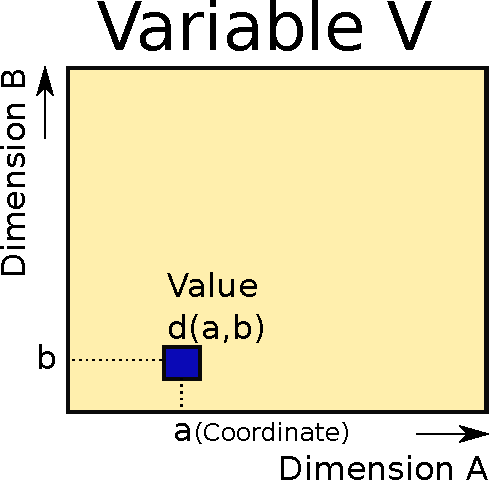
\includegraphics[width=5cm]{figures/data-model-variable}
%	\caption{Illustration of a 2D variable}
%	\label{fig:domainEntities}
%\end{figure}
% If we really want a figure, I've got a better one (BNL)



Whatever the sampling regime and dimensionality, values of of a variable $V$ will be laid out in storage. In the next section (\ref{subsec-ldm}) we present the logical data model associated with the storage, before presenting a mapping of the conceptual data model to storage in section \ref{subsec-mapping}).


\subsection{Logical Data Model}
\label {subsec-ldm}

The logical data model describes how data is represented inside ESDM, the operations to interact with the data and their semantics. There are four first class entities in the ESDM logical data model: \textbf{variable}s, \textbf{fragment}s, \textbf{container}s, and \textbf{metadata}. ESDM entities may be linked by ESDM \textbf{reference}s, and a key property which emerges from the use of references is that no ESDM entity instance may be deleted while references to it still exist. The use of reference counting will ensure this property as well as avoid dangling pointers.

\Cref{fig:data-model} gives an overview of the logical data model.



Each of these entities is now described, along with a list of supported operations:

\paragraph{Variable:} In the logical data model, the variable corresponds directly to a variable in the conceptual data model. Each element of the variable sampled across the dimensions contains data with a prescribed \textbf{DataType}.
Variables are associated with both \textbf{Scientific Metadata} and \textbf{Technical Metadata}. Variables are partitioned into \textbf{fragments} each of which can be stored on one or more ``storage backend''.
A variable definition includes internal information about the domain (bounding box in some coordinate system)  and dimensionality (size and shape), while the detailed information about which coordinate variables are needed to span the dimensions and how they are defined is held in the technical metadata.  Similarly, where a variable is itself a coordinate variable, a link to the parent variable for which it is used is held in the technical metadata.
The ESDM will not allow an attempt to delete a variable to succeed while any such references exist (see references).
A key part of the variable definition is the list of fragments associated with it, and if possible, how they are organised to span the domain.
Users may choose to submit code pieces that are then run within the I/O-path (not part within ESiWACE implementation), such an operation covers the typical filter, map and reduce operations of the data flow programming paradigm.

Fragments are created by the backend while appending/modifying data to a variable.

\textbf{Operations:}
\begin{itemize}
	\item Variables can be created and deleted.
	\item Fragments of data can be attached and deleted.
	\item Fragments can be repartitioned and reshuffled.
	\item Integrity can be checked.
	\item Data can be read, appended or modified those operations will be translated to the responsible fragments.
	\item Metadata can be atomically attached to a variable or modified.
	\item A variable can be sealed to make it immutable for all subsequent modifications.
	\item Process data of the variable somewhere in the I/O-path.
\end{itemize}

\paragraph{Fragment:}  A fragment is a piece (subdomain) of a variable. The ESDM expects to handle fragments as atomic entities, that is, only one process can write  a fragment through the ESDM, and the ESDM will write fragments as atomic entities to storage backends.
The backends are free to further partition these fragments as is appropriate, for example, by sharding using chunks as described in section \ref{subsec-mapping}.
However, the ESDM is free to replicate fragments or subsets of fragments and to choose which backend is appropriate for any given fragment.
This allows, for example, the ESDM to split a variable into fragments some of which are on stored on a parallel file system, while others are placed in object storage.

\textbf{Operations:}
\begin{itemize}
	\item Data of fragments can be read, appended or modified.
	\item Integrity of the fragment can be checked.
	\item Process data of the variable somewhere in the I/O-path.
\end{itemize}
%\todo{Resolve question on slack: \url{https://esiwace.slack.com/archives/C2T7KDRGC/p1496396797771552}}

\paragraph{Container:} A container is a virtual entity providing views on collections of variables, allowing multiple different data sets (as defined in the conceptual model) to be realised over the variables visible to the ESDM.  Each container provides a hierarchical namespace holding references to one or multiple variables together with metadata.Variables cannot be deleted while they are referenced by a container.  The use of these dynamic containers provides support for much more flexible organisation of data than provided by a regular file system semantics --- and efficiently support high level applications such as the Data Reference Syntax\footnote{Taylor et al (2012): CMIP5 Data Reference Syntax (DRS) and
Controlled Vocabularies.}.

A container provides the ESDM storage abstraction which is analogous to an external file. Because many scientific metadata conventions are based on semantic structures which span variables within a file in ways that may be opaque to the ESDM without the use of a plugin, the use of a container can indicate to the ESDM that these variables are linked even though the ESDM does not understand why, and so they cannot be independently deleted.
When entire files in NetCDF format are ingested into the ESDM, the respective importing tool must create  a container to ensure such linking properties are not lost.

\textbf{Operations:}
\begin{itemize}
	\item Creation and deletion of containers.
	\item Creation and deletion of names in the hierarchical name space; the creation of links to an existing variable.
	\item Attaching and modification of metadata.
	\item Integrity can be checked.
\end{itemize}

\paragraph{Metadata:} can be associated with all the other first class entities (variables, fragments, and containers). Such metadata is split into internal ESDM technical metadata, and external user-supplied semantic metadata.
%A future version of the ESDM will support the internal exploitation of external metadata via plugins, but this version of the ESDM will treat external metadata as atomic and opaque, and simply serialise and store/replace/delete any such metadata. The internal metadata ...
%\todo {There needs to be a formal description of internal metadata}
Technical metadata covers, for example, permissions, information about data location and timestamps.
A backend will be able to add its own metadata to provide the information to lookup the data for the fragment from the storage backend managed by it.
Metadata by itself is treated like a normal ESDM variable but linked to the variable of choice.
The implementation may embed (simple) metadata into fragments of original data (see Reference).

\textbf{Operations:}
\begin{itemize}
	\item Uses can create, read, or delete arbitrary scientific metadata onto variables and containers.
	A future version of the ESDM may support user scientific metadata for fragments.
	\item Container level metadata is generally not directly associated with variables, but may be retrieved via following
	references from variables to containers.
	\item Queries allow to search for arbitrary metadata, e.g., for objects that have (\texttt{experiment=X, model=Y, time=yesterday}) returning the variables and containers in a list that match.
	This enables to locate scientific data in an arbitrary namespace.
\end{itemize}

\paragraph{Reference}
A reference is a link between entities and can be used in many places, references can be embedded instead of real data of these logical objects.
For example, dimensions inside a variable can be references, also a container typically uses references to variables.

\textbf{Operations:}
\begin{itemize}
	\item A reference can be created from existing logical entities or removed.
\end{itemize}


%\paragraph{Set}
%A set contains objects but only one object.




\begin{figure}
	\centering
	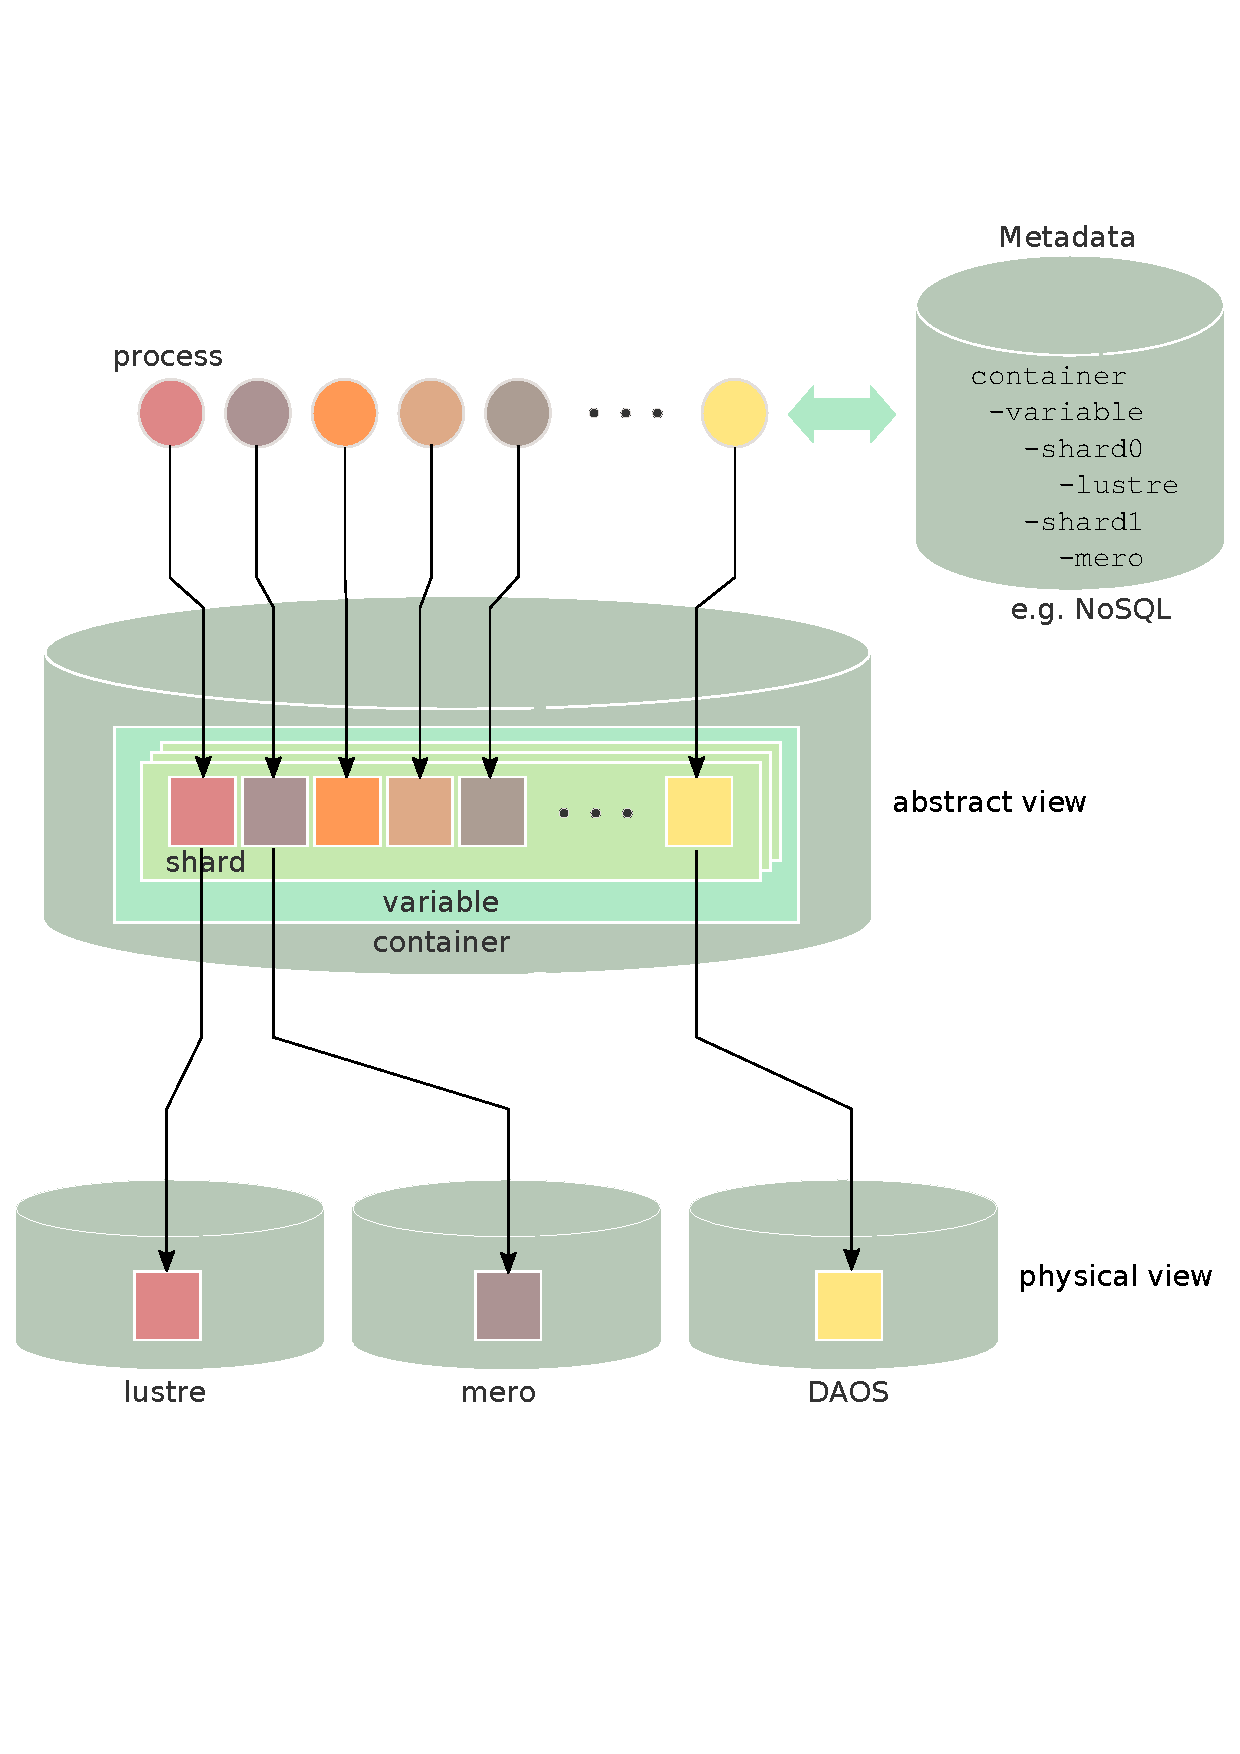
\includegraphics[width=0.5\textwidth]{data-model}
	\caption{Logical Data Model}
	\label{fig:data-model}
\end{figure}

\paragraph{Namespace}

ESDM does not offer a simple hierarchical namespace for the files.
It provides the elementary functions to navigate data: teleportation and orientation in the following fashion:
Queries about semantical data properties (e.g., \texttt{experiment=myExperiment, model=myModel, date=yesterday}) can be performed returning a list of matching files with their respective metadata.
Iterating the list (orientation) is similar to listing a directory in a file system.

Note that this reduces the burden to define a hierarchical namespace and for data sharing services based on scientific metadata.
An input/output container for an application can be assembled on the fly by using queries and name the resulting entities.
As a container provides a hierarchical namespace,
by harnessing this capability one can search for relevant variables and map them into the local file system tree, accessing these variables as if they would be, for example, NetCDF files.
By offering a FUSE client, this feature also enables backwards compatibility for legacy POSIX applications.



\subsection{Relationships between the Conceptual and Logical Data Model}
\label{subsec-mapping}

The conceptual data model and logical data model are described above, and summarised in \Cref{fig:cdm_ldm}.
These UML and this version of the architecture do not fully deal with the issues around coordinate systems which are not described by simple monotonic coordinate arrays, for which simple bounding boxes can be constructed.

As noted above, to fully exploit more complicated coordinate systems it will be necessary to describe those coordinate systems more fully in the scientific metadata (LDM\_Sci\_Metadata) and potentially provide a plugin to the system to handle them.
This notion is shown in the UML by virtue of the optional use of a named plugin to be identified in the scientific metadata, but the details of how that will work has been postponed to the prototype development.

\begin{figure}
	\centering
	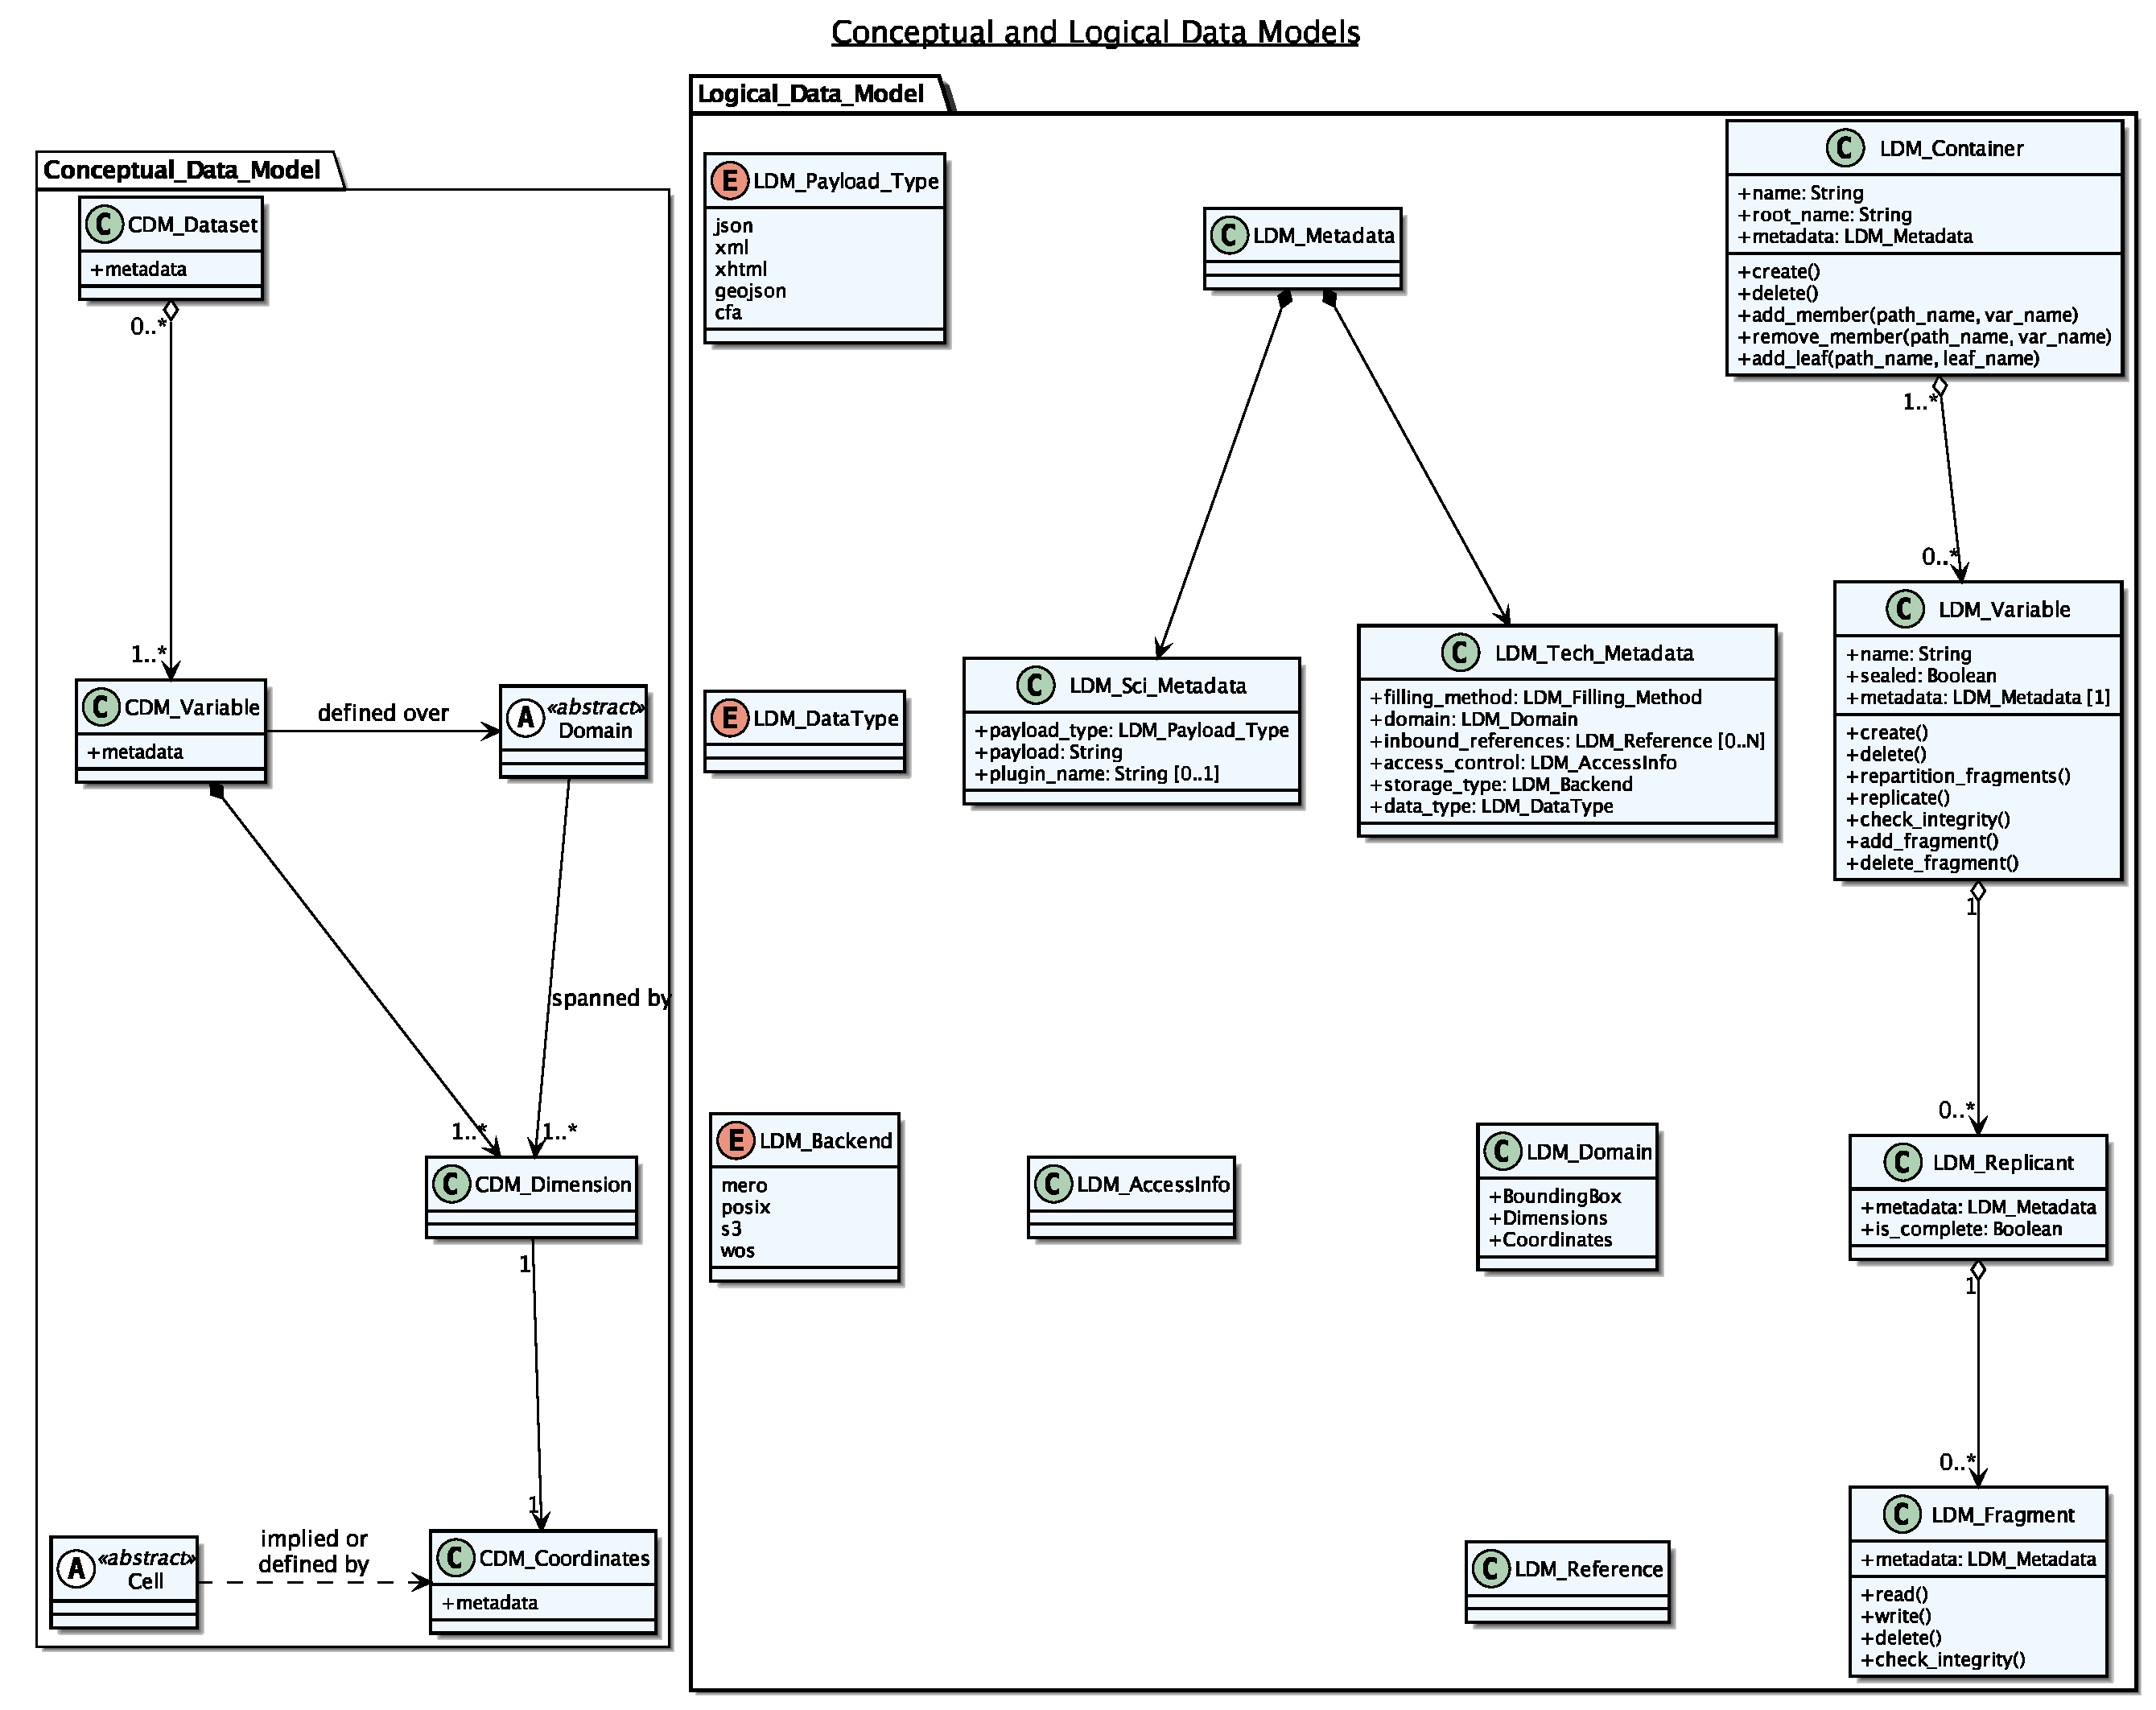
\includegraphics[width=\textwidth]{inf-model/cdm_ldm.eps}
	\caption{A non-normative UML version of the conceptual and logical data models.
	The figure includes example for the operators of the individual logical operations.
	These UML are expected to be updated as the system is developed.  See also figure \ref{fig:dm_map}.}
	\label{fig:cdm_ldm}
\end{figure}

The key high level entities are the conceptual container, variable, and domain, which have direct correspondence in the logical
data model (see \Cref{fig:dm_map}) --- however it is important to recognise that these are not isomorphic relationships. For example,
the concept of a domain of a variable in the conceptual model is expanded in the logical data model to include sub-domains associated
with fragments, but the same class is used for both usages (LDM\_Domain for both variable domain and fragment sub-domain).

\begin{figure}
	\centering
	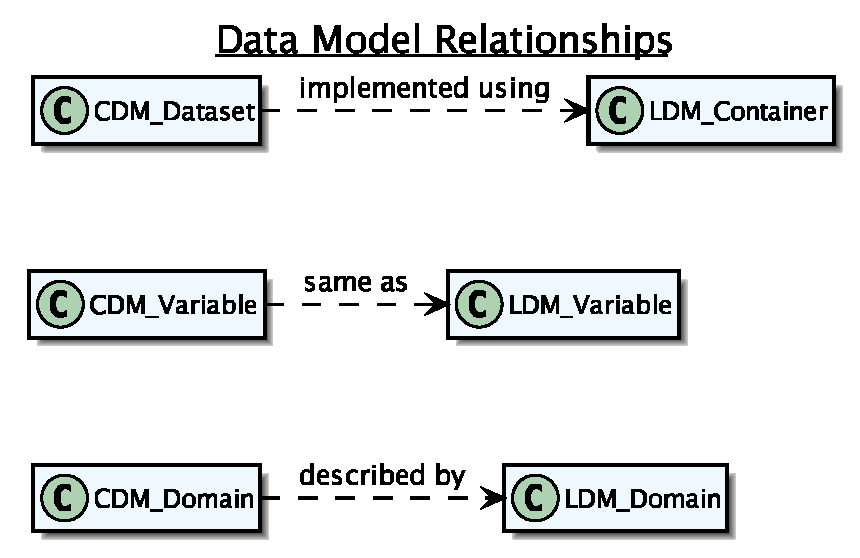
\includegraphics[scale=0.6]{inf-model/cdm_cdm.eps}
	\caption{Key relationships between conceptual and logical data models.}
	\label{fig:dm_map}
\end{figure}


%\subsection{Metadata mapping: Needs updating}
%\todo{Some examples driven from the use cases}
%

%%%%%%%%%%%%%%%%%%%%%%%%%%%%%%%%%%%%%%%%%%%%%%%%%%%%%%%%%%%%%%%%%%%%%%%%%%%%%%%
\subsubsection{Adaptive Data Mappings}
The typical storage mapping for scientific data format libraries is the file (linear sequence of bytes organized following the POSIX file system representation, i.e. inodes and blocks). Information is translated into a linear array of bytes in the file system using appropriate schemas. Since the data model defined by the data format library can contain complex hierarchies and attributes besides raw data, the final file will contain additional scientific metadata that needs to be accessed using the POSIX-IO data interface (e.g. \texttt{read()} and \texttt{write()}) instead of the file metadata interface (e.g. \texttt{stat()}, \texttt{lookup()}). This makes the storage model adopted by data format libraries incompatible with the typical parallel file system organization, in which metadata and data are splitted apart and assigned to different services for optimal performance. Additionally, new storage system paradigms have emerged in the last years in which files are organized in a flat namespace (e.g. object storage), removing the restrictions imposed by metadata operations like namespace traversal of POSIX file systems. Hierarchical organization can be still achieved using other dedicated storage representations like key-value stores, at the expense of reduced POSIX semantic.

There is therefore a necessity for more flexible data mappings that can take advantage of an increasing number of storage and backend alternatives, improving access efficiency at the same time. There are two different approaches to this problem: the first is to develop a new data mapping schema for every storage backend. This is the solution adopted by the HDF5 library (through the virtual file and the virtual object layers) in which multiple storage backends can be employed by developing a corresponding plugin that contains the right mapping schema. The obvious limitation of this solution is that once the user has selected a certain backend for a file, this cannot be changed without migrating the whole file to another backend. The second approach is more flexible and consists in making the storage backend selection adaptive. This has the advantage of enabling backend storage selection on the fly depending upon the type of data being stored or a set of user/system defined parameters (e.g. list of data placement policies satisfying certain requirements of quality of service).

Our proposed solution is to integrate the adaptive data mappings capabilities just discussed in the layout component of the ESD middleware. The middleware will understand the scientific metadata of other relevant data format libraries and will be able to use multiple storage backends at the same time to store and retrieve different pieces of data. To support multiple formats the datatype component in the ESD middleware will expose a datatype interface similar to the one available in HDF5 (described in Section~\ref{sec: data-formats}). Additionally, the middleware will add significant metadata to be used in the life cycle management and sharing of data. This can include semantic metadata describing which data is needed and how it is going to be used, the required level of resilience, etc. In this context, some metadata can be automatically generated by the middleware or defined by the user and passed to the middleware through an apposite interface (that will be part of the ESD exposed interface).

Legacy codes will have access to data using a familiar POSIX interface exported through an ESD FUSE module. The FUSE module will communicate with the ESD middleware to access data and export it to users using a namespace representation. The mapping schema definition for mapping data between the storage representation and the namespace will be done later in the project.

Another important aspect to consider when talking about adaptive data mappings is the storage tiering, that is, how many levels of storage there are in the system. Historically, HPC applications have relied on parallel file systems as first tier to store and retrieve their data. Besides the parallel file system, most high-end clusters have a second level of archival storage to which data is migrated from the parallel file system using a hierarchical storage manager. Nowadays compute nodes have access to local storage (typically a block device formatted with a local file system) and with the emergence of new storage technologies, such as non-volatile memories, permanent byte addressable memory. The ESD middleware should be able to exploit these local storage resources to implement prefetching strategies (read patterns) and burst buffers (write patterns).

%In the specific case of Mero (Seagate object store system), which represents one of the possible storage backends that has to be supported by the ESD middleware, hierarchical and semantic metadata can be stored in the key-value store service while array data can be stored into objects. In fact, we can think about using more than one object per dataset. This is particularly useful with chunking since every chunk in the dataset can be mapped to a different object, making parallel access to different data units possible without any need for I/O coordination (no false sharing is possible in this case). Of course, I/O coordination still needs to be provided when multiple processes access the same dataset and chunking is not enabled. In this case the ROMIO library already provides a collective I/O implementation that can be reused by the ESD middleware. Whenever needed, false sharing of data can also be avoided by using `persistent file realm' like mechanisms\footnote{This mechanism allows a certain file portion to be assigned to a specific process in the application and makes this assignment persistent across multiple data accesses.}.

%\todo{Giuseppe: you had a very good document on this already can add something here}

%Goal of the dynamic mapping is to create a hierarchical namespace based on the available metadata.
%It is based on the search for objects.
%With the help of FUSE, these mappings can be created based on a user configuration upon mount-time (supports user mounts).
%Inaccessible data, i.e., where the permissions are not sufficient, can be hidden from the namespace.

%An example mapping could be:
%“v.info.model/v.info.environment.date/v.info.experiment.tags/v.info.name <as NC4>”.
%This would show a single NetCDF4 file for each variable.
%If a variable is attached to various tags, then it is shown for each of them.

%“v.info.model/v.info.environment.date/v.domain.time/v.info.name <as NC4>”.
%Would show one file per timestep.

%How to resolve ambiguity?

%Existing containers can also be directly mapped, showing the input and output variables similarly:
%“<c.\_id>/<c.directory>”


%The storage should now how the logical data space maps to physical positions in memory or storage.
%If the storage backends have this knowlege, they can run local operations on the data.

%Alternatives:
%Triangular grid (locally refined), somehow mapped from user-space to a 1D structure which gets mapped to the storage. (Traditional approach)

%Application(data structure) - Mapping - Middleware - Mapping (byte array) - Storage API - Storage backend

%or:

%Application - Middleware - Storage API - Mapping - Storage backend

%Use sth. like MPI datatypes to descripe memory (in the application)
%Add metadata to describe the meaning / semantics, additional gain: resilience because we know which data to replicate to put into triple ECC ...
%Add hints how the data is used / will the used in the future

%Avoid redundant descriptions of memory / storage.
%Users stores a 3D field, it is clear which storage location is responsible for [x,y,z]
%How to store triangles etc.

%Why not store code as description?
%- describes neighborhood?

%Coordinates? Universal coordinates, application coordinates?

%VTK? haben diverse Datenstrukturen hierfÃŒr.


%Separation of concerns...

%Missmatch of Chunks size and application domain

%false sharing

%Pointer Datentyp: strong ptr, weak ptr.
%like Boost usw.


%NVRAM



%%%%%%%%%%%%%%%%%%%%%%%%%%%%%%%%%%%%%%%%%%%%%%%%%%%%%%%%%%%%%%%%%%%%%%%%%%%%%%%
\subsubsection{Technical Metadata}
\label{subsec: technical metadata}

Besides scientific metadata, the dynamic mapping of data to storage backends requires further metadata that must be managed.
To distinguish technical metadata from scientific metadata, an internal namespace is created.
Relevant metadata is shown in \Cref{tbl:additionalTechnicalMetadata} for shards, variables and containers, respectively.

Metadata can be optional (O) or mandatory (M), and either is created automatically or must be set manually via the APIs.
Automatic fields cannot be changed.
Some of the data can be automatically inferred if not set manually, but manual setting may allow further optimizations.

Some of the metadata is used on several places, for example, information about the data lineage might be used to create several output variables.
In our initial implementation, the metadata is stored redundantly as this:
1) simplifies search; 2) enables us to restore data on corrupted storage systems by reading the metadata; 3) reduces contention and potentially false sharing of metadata.
An implementation might decide to reduce this by utilizing a normalized schema.

References is the list of objects that are directly used by this object, e.g., other variables that are used to define the data further.

\begin{table}
\begin{subtable}[t]{\textwidth}
\begin{tabular}{llll}
Metadata & Field & Creation & Description\\
\hline
Domain   & M & Auto & The subdomain this data covers from the variable\\
Type     & M & Auto & The (potentially derived) datatype of this shard\\
Variable & M & Auto & The ID of the variable this data belongs to\\
Storage  & M & Auto & The storage backend used and its options\\
References & M & Auto & A list of objects that are referenced by this data\\
Sealed   & M & Auto & A sealed shard is read-only\\
\end{tabular}
\caption{For a shard}
\end{subtable}

\begin{subtable}[t]{\textwidth}
\begin{tabular}{llll}
Metadata & Field & Creation & Description\\
\hline
Domain      & M & Manual & Describes the overall domain\\
Type   	    & M & Manual & The (potentially derived) datatype\\
Info   	    & M & Manual & The scientific metadata of this document\\
References  & M & Auto & A list of objects that are referenced by this data\\
Permissions & M & Auto/Manual & The owner and permissions \\
Shards      & M & Auto & The list of shard objects for this variable\\
Sealed      & M & Auto & A sealed variable is read-only\\
\end{tabular}
\caption{For a variable}
\end{subtable}

\todo{
	6.X Mero => TODO Seagate
	6.X HDF5+MPI plugin
	* Typical run as MPI+HDF5 application ?
	** Master process, setup files?
	** Beispiel: Workflows using the containers => aus dem Use Case
	"Pipelines/Workflows"
}

\begin{subtable}[t]{\textwidth}
\begin{tabular}{llll}
Metadata & Field & Creation & Description\\
\hline
Owner    & O     & Manual   & The owner of this file view (see the permission model)\\
Info     & O     & Manual   & Additional scientific metadata for this view\\
Directory & O    & Manual   & Contains a mapping from names to variables\\
Environment & O  & Automatic & Information about the application run\\
Permissions & M & Auto/Manual & The owner and permissions \\
References  & M & Auto & A list of objects that are referenced by this data.
\end{tabular}
\caption{For a container}
\end{subtable}
\caption{Excerpt of additional technical metadata}
\label{tbl:additionalTechnicalMetadata}
\end{table}


\paragraph{Example}

This example illustrates data of a predictive model could be stored on the system and the resulting metadata.
The dimensionality of the underlying grid is fixed.

The application uses the following information to drive the simulation:
\begin{itemize}
 \item Timerange: the simulated model time (from a starting datetime to the specified end)
 \item Longitude/Latitude: 1D data field with the coordinates [float]
 \item Temperature: Initial 2D field defined on (lon, lat)
\end{itemize}
A real model would use further parameters to estimate the temperature but these are sufficient to demonstrate the concepts.
This information is either given as parameter to the simulation or read from an input (container).
A mixture of both settings is possible.


The application produces the following output:
\begin{itemize}
  \item Longitude/Latitude: 1D data field with the coordinates [float]
  \item Model time: the current time inside the simulation
  \item Temperature: 2D field defined on (lon, lat, time) [float], containing the precise temperature on the coordinates defined by lon and lat for the given timestep
  \item AvgTemp: 1D field defined on (time) [float]; contains the mean temperature for the given time
\end{itemize}


Upon application startup, we create a new virtual container that provide links to the already existing input.
In \Cref{lst:mongoContainer}, the metadata for the container is shown, after the application is started.
We assume it has used the APIs to provide the information (input, output, scientific metadata).
In this example, we explicitly define the objects used as input; it is possible to also define
the input as an already existing container.
It is also possible to define the input a-priori if the objectIDs are known / looked up prior application run.
The intended output variables could be given with their rough sizes.
This would allow the scheduler to pre-stage the input and ensure that there is enough storage space available for the output.
The environment information is inferred to the info object but can be changed from the user.

\begin{tcbcode}[label={lst:mongoContainer}]{JSON document describing the container}
\begin{lstlisting}
"_id" : ObjectId(".."),
"directory" : {
  "input" : {
    "longitude" : ObjectId(".."),
    "latitude" : ObjectId(".."),
    "temperature" : ObjectId("..")
   },
  "output" {
     "temperature" : ObjectId(".."),
     "avgTemp" : ObjectId("..")
   }
},
"info" : {
  "model" : { "name" : "my model", "version" : "git ...4711" },
  "experiment" : {
    "tags"        : ["simulation", "poisson", "temperature"]
    "description" : "Trivial simulation of temperature using a poisson process"
  },
},
"environment" : {
  "date"  : datetime(2016, 12, 1),
  "system" : "mistral",
  "nodes" : ["m[1-1000]"]
},
"permissions" : {
  "UID"  : 1012,
  "GID"  : 400,
  "group" : "w", # allows read also
  "other" : "r"
},
"references" : {
  [ all links to used object IDs from input / output ]
}
\end{lstlisting}
\end{tcbcode}

The metadata for a single variable is build based on the information available in the container and additional data provided by the user.
An example for the temperature variable is shown in \Cref{lst:mongotemperature}.
When describing the domain that is covered by the variable, there are two alternatives:
1) a reference to an existing variable is embedded and the minimum / maximum value is provided.
This allows to reuse descriptive information as data has to be stored only once. Min and max describe the multidimensional index of the subdomain in the variable that is actually referenced;
2) data becomes embedded into the file. This option is used when the size of the variable is small.

An advantage of option 2) is that searches for data with a certain property do not require to lookup information in additional metadata.

Similarly, information about the data lineage (history) can originally be inferred from the objects linked in the directory mapping.
The metadata of the referenced object must be copied, if the original object is removed.

\begin{tcbcode}[label={lst:mongotemperature}]{JSON document for temperature}
\begin{lstlisting}
"_id" : ObjectId("<TEMPID>"),
"sealed" : true,
"domain" : [
    "longitude" : [ "min" : 0, "max" : 359999, "reference" : ObjectId("..") ],
    "latitude" : [ "min" : 0, "max" : 179999, "reference" : ObjectId("..") ],
    "time" : [ datetime(...), datetime(...), ... ]
  ],
"type" : "float",
"info" : {
  "convention" : "CF-1.0",
  "name" : "temperature",
  "unit" : "K",
  "long description" : "This is the temperature",
  "experiment" : {
    "tags"        : ["simulation", "poisson", "temperature"]
    "description" : "Trivial simulation of temperature using a poisson process"
  },
  "model" : { "name" : "my model", "version" : "git ...4711" },
  "directory" : {
	"input" : {
	  "longitude" : ObjectId("<LONID>"),
	  "latitude" : ObjectId("<LATID>"),
	  "temperature" : ObjectId("<TEMPID>")
	}
  },
  "environment" : {
    "date"    : datetime(2016, 12, 1),
    "system" : "mistral",
    "nodes"  : ["m[1-1000]"]
  },
  "history" : [
  To illustrate the applied mapping, we use a subset of our NetCDF metadata described in \Cref{sec:netcdfDataMapping}.
  The excerpt is given in \Cref{lst:NetCDF-data-map}.
  The mapping of a single logical variable is exemplarily described in


  \begin{tcbcode}[label={lst:NetCDF-data-map}]{NetCDF metadata for one variable}
  \begin{lstlisting}
  dimensions:
  longitude = 480 ;
  latitude = 241 ;
  time = UNLIMITED ; // (1096 currently)
  variables:
  float longitude(longitude) ;
  longitude:units = "degrees_east" ;
  longitude:long_name = "longitude" ;
  float latitude(latitude) ;
  latitude:units = "degrees_north" ;
  latitude:long_name = "latitude" ;
  int time(time) ;
  time:units = "hours since 1900-01-01 00:00:0.0" ;
  time:long_name = "time" ;
  time:calendar = "gregorian" ;
  short sund(time, latitude, longitude) ;
  sund:scale_factor = 0.659209863732776 ;
  sund:add_offset = 21599.6703950681 ;
  sund:_FillValue = -32767s ;
  sund:missing_value = -32767s ;
  sund:units = "s" ;
  sund:long_name = "Sunshine duration" ;

  // global attributes:
  :Conventions = "CF-1.0" ;
  :history = "2015-06-03 08:02:17 GMT by grib_to_netcdf-1.13.1: grib_to_netcdf /data/data04/scratch/netcdf-atls14-a562cefde8a29a7288fa0b8b7f9413f7-lFD4z9.target -o /data/data04/scratch/netcdf-atls14-a562cefde8a29a7288fa0b8b7f9413f7-CyGl1B.nc -utime" ;
  }
  \end{lstlisting}
\end{tcbcode}

To simplify search and identify data clearly, data services such as the WDCC and CERA, that offer data to the community, request scientists to provide additional metadata.
Normally, such data is provided when the results of an experiment is ingested into such a database.
Example metadata is listed in \Cref{tbl:additionalMetadata}.
In existing databases, the listed metadata is split into several fields, e.g. an address and email for persons, for simplicity only a rough overview is given.
Instead of encoding the history as a simple text field, it could
indicate detailed steps including the arguments for the commands and versions and transformations to reproduce the data.
This should include for each step, where and the ti
    #The history for the inputs, if the data lineage must be embedded
    ObjectId(<LONID>) : [
      # Assume LONID does not exist any more
    ],
  ]
},
"permissions" : {
  "UID"  : 1012,
  "GID"  : 400,
  "group" : "w", # allows read also
  "other" : "r"
},
"references" : {
  [ all links to used object IDs ]
},
"shards" : [
  ObjectId(<SHARD1 ID>),
  # For a sealed object, the domains of its shards can optionally be embedded:
  { "reference" : ObjectId(<SHARD2 ID>), "storage" : ... , "domain" },
  ObjectId(<SHARD3 ID>),
  ObjectId(<SHARD4 ID>)
]
\end{lstlisting}
\end{tcbcode}

The variable is split into multiple shards; metadata for one of them is shown in \Cref{lst:mongotemperatureshard}.
Since we assume domain decomposition in the application, the longitude and latitude variables are now only partially stored in a shard.
In the example, we assume two processes create one shard each and the surface of the earth is partitioned into four non-overlapping rectangles.

\begin{tcbcode}[label={lst:mongotemperatureshard}]{JSON document for a shard of the temperature variable}
\begin{lstlisting}
"_id" : ObjectId("<SHARD1 ID>"),
"sealed" : true,
"variable" : ObjectId("<TEMPID>"),
"type" : "float",
"domain" : {
    "longitude" : [ "min" : 0, "max" : 179999, "reference" : ObjectId("..") ],
    "latitude" : [ "min" : 0, "max" : 89999, "reference" : ObjectId("..") ],
    "time" : [ datetime(...), datetime(...), ... ]
  },
"storage" : {
    "plugin" : "pfs",
    "options" : {
      "path" : "/mnt/lustre/testdir/file1",
    },
    "serialization" : "row-major"
  },
"references : [
  ObjectId("<TEMPID>"),
  ObjectId(".."),
  ObjectId("..")
]
\end{lstlisting}
\end{tcbcode}



%%%%%%%%%%%%%%%%%%%%%%%%%%%%%%%%%%%%%%%%%%%%%%%%%%%%%%%%%%%%%%%%%%%%%%%%%%%%%%%
\subsection{Data/Metadata Backend Drivers}
A prototypical metadata backend will be realized using MongoDB.
Advantages of using MongoDB are that it scales horizontally with the number of servers, provides fault-tolerance and that the document model supports arbitrary schemas.



To illustrate the applied mapping, we use a subset of our NetCDF metadata described in \Cref{sec:netcdfDataMapping}.
The excerpt is given in \Cref{lst:NetCDF-data-map}.
The mapping of a single logical variable is exemplarily described in


\begin{tcbcode}[label={lst:NetCDF-data-map}]{NetCDF metadata for one variable}
\begin{lstlisting}
dimensions:
	longitude = 480 ;
	latitude = 241 ;
	time = UNLIMITED ; // (1096 currently)
variables:
	float longitude(longitude) ;
		longitude:units = "degrees_east" ;
		longitude:long_name = "longitude" ;
	float latitude(latitude) ;
		latitude:units = "degrees_north" ;
		latitude:long_name = "latitude" ;
	int time(time) ;
		time:units = "hours since 1900-01-01 00:00:0.0" ;
		time:long_name = "time" ;
		time:calendar = "gregorian" ;
	short sund(time, latitude, longitude) ;
		sund:scale_factor = 0.659209863732776 ;
		sund:add_offset = 21599.6703950681 ;
		sund:_FillValue = -32767s ;
		sund:missing_value = -32767s ;
		sund:units = "s" ;
		sund:long_name = "Sunshine duration" ;

// global attributes:
		:Conventions = "CF-1.0" ;
		:history = "2015-06-03 08:02:17 GMT by grib_to_netcdf-1.13.1: grib_to_netcdf /data/data04/scratch/netcdf-atls14-a562cefde8a29a7288fa0b8b7f9413f7-lFD4z9.target -o /data/data04/scratch/netcdf-atls14-a562cefde8a29a7288fa0b8b7f9413f7-CyGl1B.nc -utime" ;
}
\end{lstlisting}
\end{tcbcode}

To simplify search and identify data clearly, data services such as the WDCC and CERA, that offer data to the community, request scientists to provide additional metadata.
Normally, such data is provided when the results of an experiment is ingested into such a database.
Example metadata is listed in \Cref{tbl:additionalMetadata}.
In existing databases, the listed metadata is split into several fields, e.g. an address and email for persons, for simplicity only a rough overview is given.
Instead of encoding the history as a simple text field, it could
indicate detailed steps including the arguments for the commands and versions and transformations to reproduce the data.
This should include for each step, where and the time when it is performed, and the versions of software used.

It is easily imaginable that most of this information could be useful already when the data is created as it simplifies the search and data management on the online storage.
Some of the data fields become only available after the initial data creation, e.g., the DOI.
Potentially the data must be updated / curated after the data is created.

\begin{table}
\begin{tabular}{ll}
Metadata & Description\\
\hline
Project & The scientific project during which the data is created \\
Institute & The institution which conducted the experiment\\
Person &  A natural person; could be a contact, running the experiment \\
Contact & Reference to person or consortium \\
DOI      & A document object identifier; useful for identifying a data publication\\
Topic     & Some information about the topic of the data / experiment \\
Experiment & Description of this particular experiment \\
History & A list with the history and transformations conducted with the data \\
\end{tabular}
\caption{Excerpt of additional scientific metadata}
\label{tbl:additionalMetadata}
\end{table}





\subsection{Data types}
\label{sec: viewpoints/logical/datatypes}


The ESD middleware is specifically designed for weather and climate applications.
These applications usually use GRIB and NetCDF as data format to send and store
data. Nevertheless, the middleware should be also able to support other types of
applications that use arbitrary libraries to represent and store data.

The NetCDF and HDF5 libraries define their own atomic and basic data types and
then provide the APIs to build user defined data types from these. Generally
speaking it makes sense to support a restricted number of most common data types
that application can use out of the box and offer the possibility of extending
these by means of additional APIs.

The support of native data types like H5T\_NATIVE\_INT or NC\_INT is driven by the necessity to decouple the internal representation of the data from the way data is ultimately stored.
Using native data types data can be correctly reconstructed passing from one representation to another.
Like other libraries, the ESD middleware will also support a restricted range of native data types and a series of dedicated APIs to build user defined data types.

\medskip

ESDM will support various atomic data types, integers, floating points, with
different width, precision, endian and sign. The following table lists the
possible atomic data types:

\begin{center}
	\begin{tabular}{|c|c|}
		\hline
		type & description \\
		\hline
		ESDM\_T\_I8     & char                           \\
		ESDM\_T\_U8    & unsigned char                  \\
		ESDM\_T\_I16    & short (16bit)                  \\
		ESDM\_T\_U16   & unsigned short (16bit)         \\
		ESDM\_T\_I32      & integer (32bit)                \\
		ESDM\_T\_U32     & unsigned int (32bit)           \\
		ESDM\_T\_I64    & long long (64bit)              \\
		ESDM\_T\_U64   & unsigned long long (64bit)     \\
		ESDM\_T\_F16    & float (16bit)                  \\
		ESDM\_T\_F32    & float (32bit)                  \\
		ESDM\_T\_F64   & double (64bit)                 \\
		ESDM\_T\_F128 & long double (128bit)           \\
		ESDM\_T\_TIMESTAMP & Date and time stamp \\
		\hline
	\end{tabular}
\end{center}

User defined complex data types include compound, variable length array,
and array (fixed length array).
Compound is similar to a struct in the C language.
It is an aggregation of members, which are atomic data types or other complex
data types.
Array has fixed number of base data types, which are atomic data types
or other complex data types.
A variable-length array has a flexible length of base data types.

The definition of user defined data types have to be stored on back-end. When
reading data from data sets, these data types definition is retrieved from back-end
and parsed, and proper in-memory data structures and memories are allocated to
accommodate the expected data points.
Complex data types are encoded and stored on back-end in various formats according
to different back-end.
For example, for the Mero backend, these definition will be stored in Key/Value pair in index.
The datatype is integral part of the stored variable and fragment to allow the storage backend to understand the data and process it on demand (not part of the ESiWACE project).
\Cref{fig:datatypes} lists the required interfaces for compound, array and key value based data structures.



\begin{figure}
	\centering
	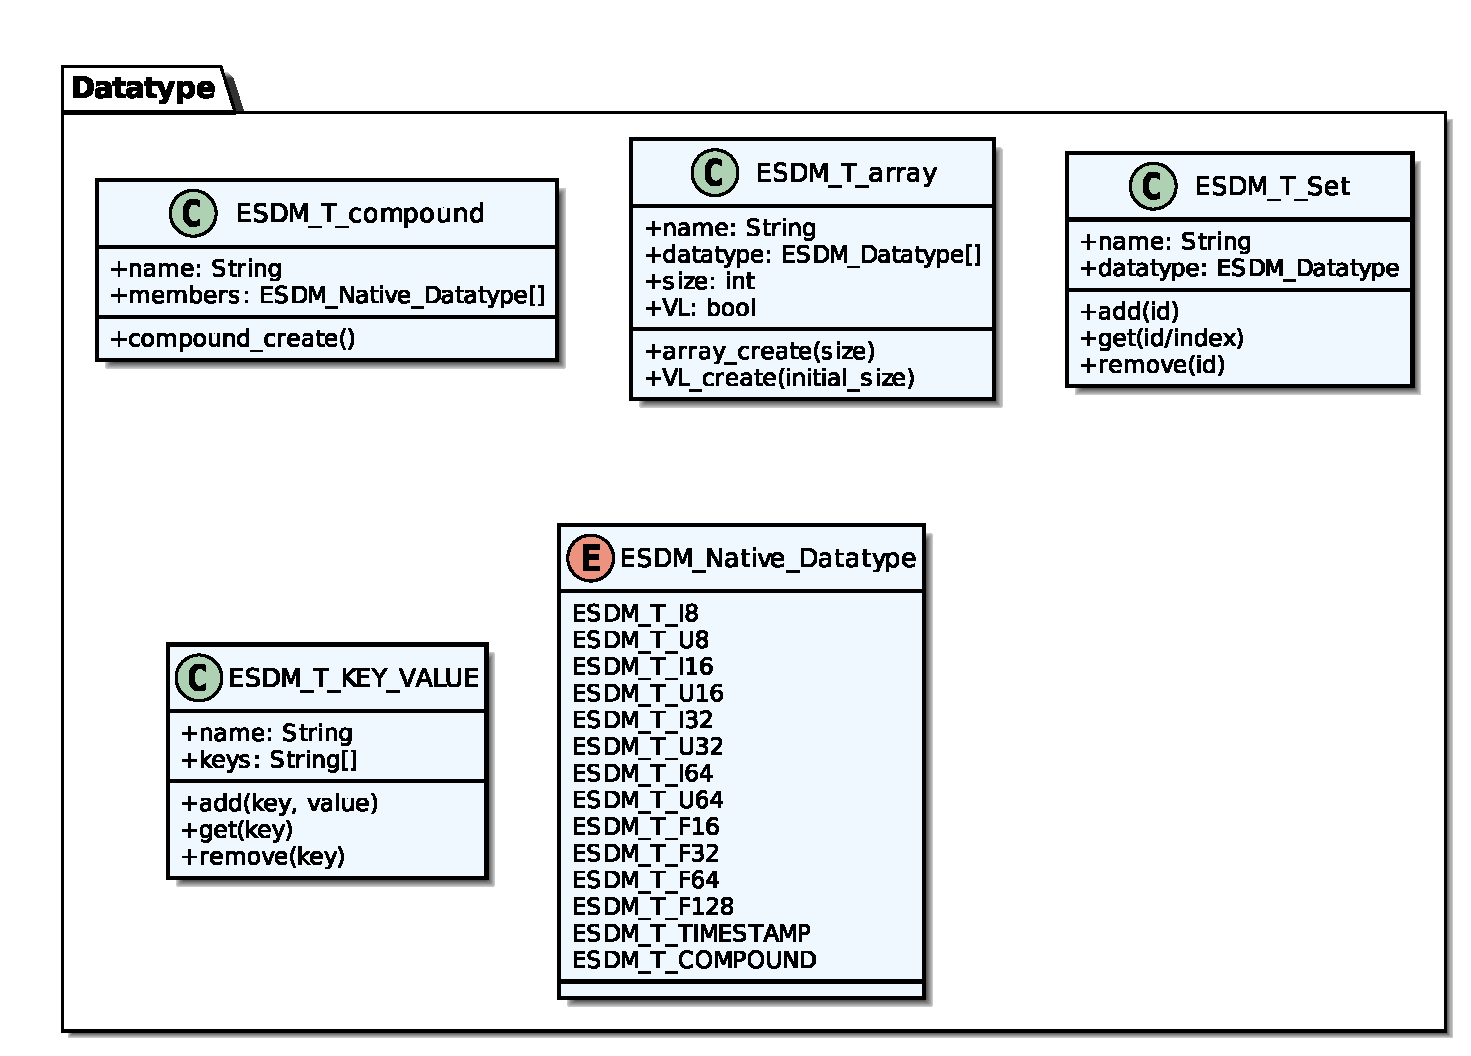
\includegraphics[width=0.9\textwidth]{esdm-semantics/semantics-datatypes.eps}
	\caption{Interfaces for the compound, array and key-value based data structures in relation to ESDM native data types.}
	\label{fig:datatypes}
\end{figure}









%%%%%%%%%%%%%
\clearpage
\section{Operations and Semantics}
\label{sec: viewpoints/logical/semantics}


\begin{figure}
	\centering
	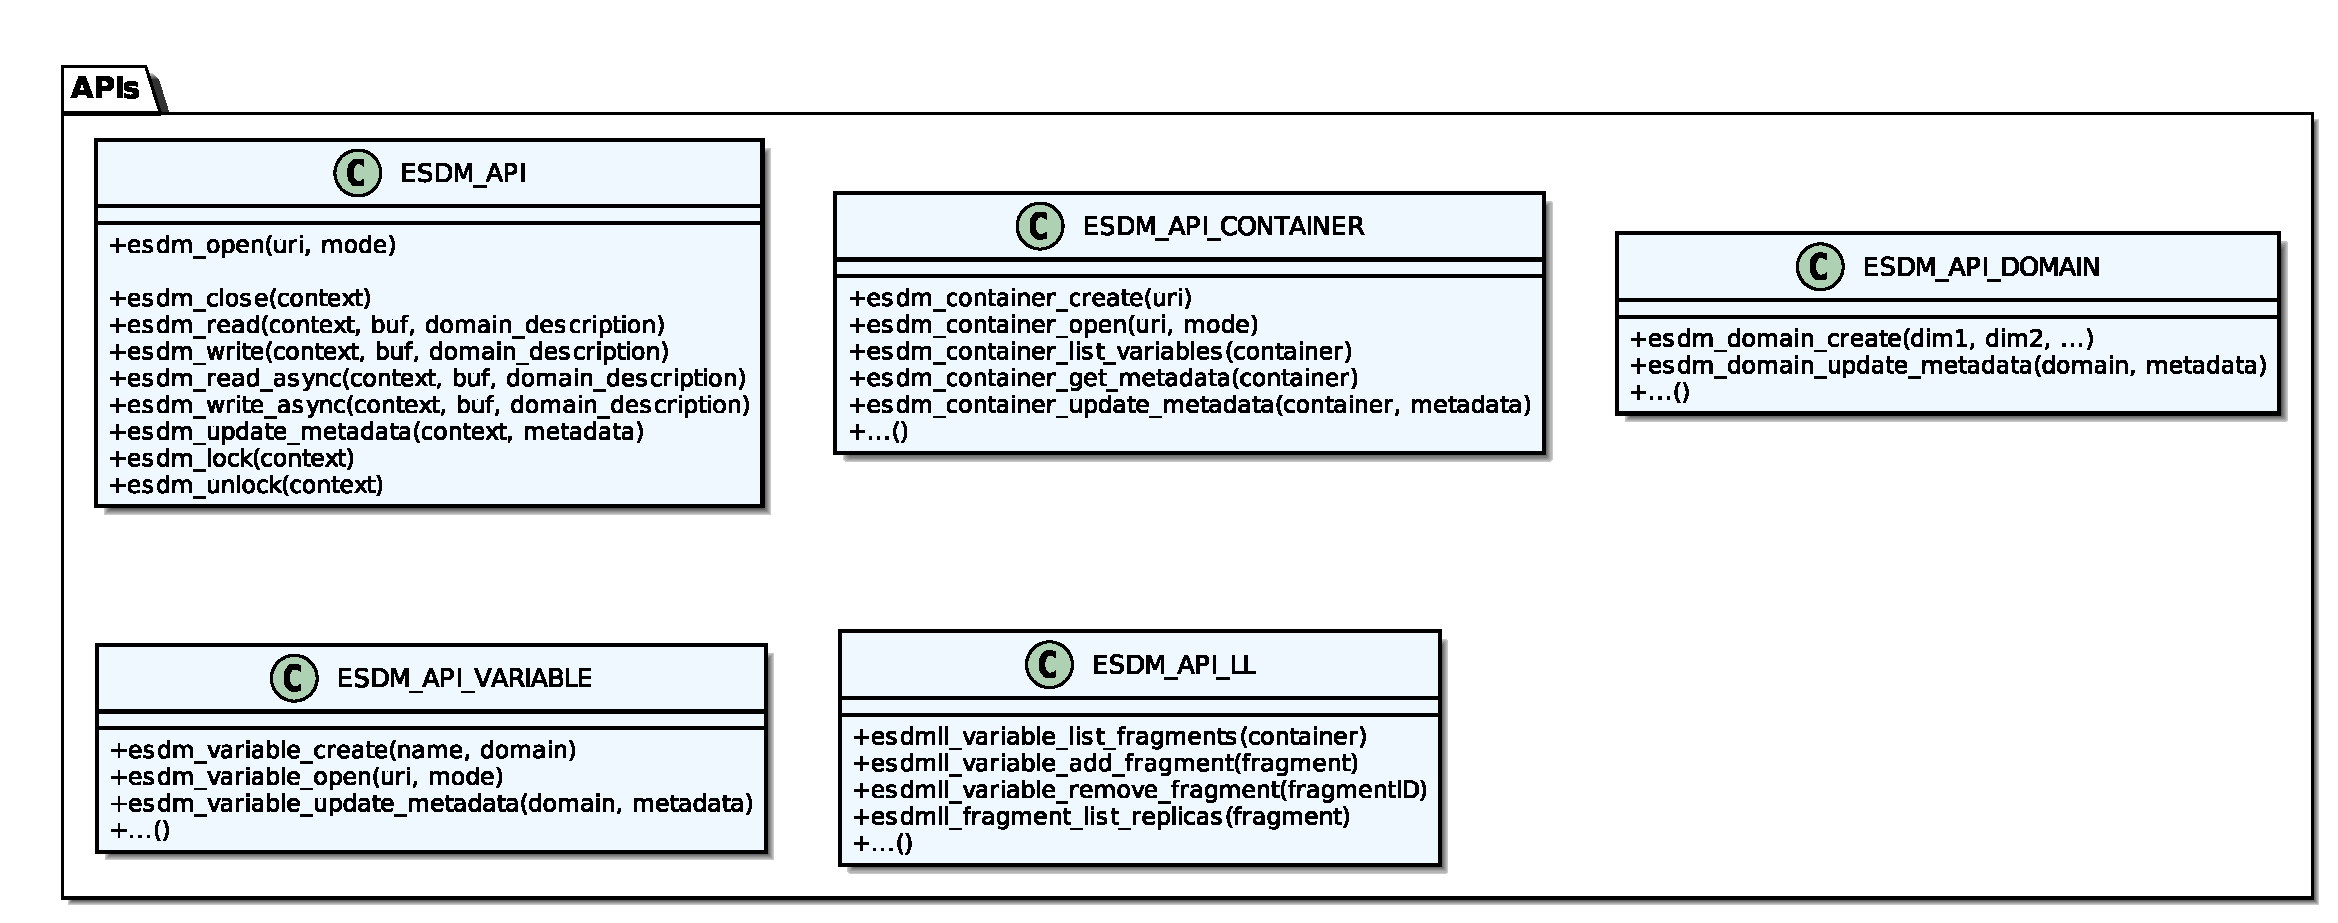
\includegraphics[width=\textwidth]{esdm-semantics/semantics.eps}
	\caption{The low and high level interfaces for standard interactions with the ESDM.}
	\label{fig:apis ll and high}
\end{figure}

This section collect the most important high-level and low-level APIs and allowed operations on ESDM data structures.
The ESDM should handle failures and many fragmentation related decisions as transparently as possible while offering a more expressive I/O API for structured data.
The conceptual model (see \Cref{subsec: conceptual data model}) does not provide the notion of files, however, some concepts familiar from file systems are also available in the ESDM system:
\begin{itemize}
\item Grouping: When existing applications are dealing with files, the ESDM will ensure that a container is available which maps onto the application view of that file.
\item Naming and Pointing: It is necessary to name things and point to them.
For a traditional file this is accomplished using a name and a file system path.
For the ESDM, we allow providing a URI which would resolve to a virtual container description or that allows to construct a virtual container on the fly linking all needed variables into it.
This is achievable because URIs are also available for all variables within a file.
\end{itemize}


\paragraph{Accessing data}

The API provides means to start reading and modification of data asynchronously and offers a \texttt{wait()} call to block until a particular operation terminates.
While the read/write is ongoing the data in memory that is read/or write must not be changed by the application, otherwise the result is undefined.

The ESDM does not support concurrent read and write scenarios, data can only be written or read (see Epoch), so the use of the ESD has one important ramification for application views of files:
\begin{itemize}
\item All interfaces which exploit the ESDM middleware will only allow file open to either read or write, but not both at the same time.
\item There can only be a single application that writes to a particular variable or fragment.
We expect that an application is using some kind of coordination mechanism to cooperate on reading and writing (more details will follow).
\item One application may write data while another reads data that has been previously written (in one previous epoch).
\end{itemize}
%\todo{Is that really what we mean?  See the todo wrt to fragment updates. This last point may need modification.}


\paragraph{Sealed Variables/Containers} ensure that data products are preserved and cannot be modified, thus URIs to these objects can typically be safely exchanged with peers.
The system may use this information to provide even more aggressive optimisations on read patterns.

\bigskip


In \Cref{fig:apis ll and high} provides an overview to the available ESDM core interfaces.
The following groups of interfaces can be distinguished:

\paragraph{Accessing existing data structures:}
ESDM data structures such as containers and variables maybe opened using an open call using a object identifier or a URI.
Likewise, it is possible to close a structure again.
A data structure has to be created before it is possible to read and write data.

\paragraph{Creation of data structures:}
The information necessary to create a ESDM data structure vary, therefore, each provides special methods to conveniently create the data structure.
It is possible to attach metadata to certain data structures such as variables and containers as they are created.


\paragraph{Exclusive access and concurrency control:}
A single parallel application may temporarily transfer own a container or variable exclusively using a locking mechanism.
This is necessary to facilitate data restructuring to rebuild upon failures or redistribute and optimise the data structures under the hood.
To allow scaling, it is sufficient that a single process of the (parallel) application maintains the lock.
Locks will timeout to prevent permanent deadlocks.
Synchronisation happens through the HDF5/MPI Vol plugin (see \Cref{frontend: hdf5 + mpi}) but may be implemented as a lightweight  library on top of MPI as well.
Any other parallel programming language should implement such a library to reduce the burden while performing certain (traditionally metadata sensitive) operations.
For efficient parallel write access, epoch semantics are available which are discussed in more detail in \Cref{sec: viewpoints/logical/data model/epochs}.
Open structures implicitly are attached with a communication channel by using events and notifications to notify upon changes in the epoch and prevent polling.
The event and notification facilities of ESDM are discussed in \Cref{sec: viewpoints/logical/data model/notification}.


\paragraph{Low level interfaces:}
In some cases, it can be more efficient to interact with the low level data structures provided by ESDM directly.
This may be the case when ESDM may not yet provide data abstractions that fit the application.
In this case developers can use the low level APIs to also access ESDM internal structures.
A direct manipulation is not possible and has to occur through an ESDM interface to ensure consistency.






%%%%%%%%%%%%%%%%%%%%%%%%%%%%%%%%%%%%
\subsection{Epoch Semantics}
\label{sec: viewpoints/logical/data model/epochs}

To allow applications developers and ESDM frontends to efficiently exploit concurrency the ESDM offers epoch semantics.
An epoch is an instant in time chosen by the parallel application.
\Cref{fig:epoch semantics} illustrates the ESDM methods to interact with epochs and also illustrates how the most recent readable view is reconstructed.
Starting with epoch 0, all processes of the parallel application participating in I/O have to agree on moving to a new epoch.
This will finalise the outstanding write requests, make the changes durable and publish the information about new data to other applications that registered to read this data.
Writing data follows the expected semantics for writes but when multiple writers update data from the same variable coordinates, i.e., they overwrite data, the result is undefined.
In fact, applications of which multiple processes write in the same epoch to the same data region are considered to be wrong.

Closing a variable or finalising ESDM will also move it to the next Epoch, thus finalise the first version.
Writing data to a variable that existed previously will overwrite the data of previous epochs.
Similarly, if a variable is opened for read/write access, the same application may now read the data from a previous epoch.
Reading data that has been written by another process of the same application (i.e., a read after write) should be prevented, as users should use means of communication inside the application to prevent this kind of access pattern.
Thus, a read request will never return the data of the current epoch but the merged perspective of all previous epochs.
In that sense, the epoch semantics is similar to the semantics of transactions but application wide and only one transaction can be active at a given time.
If a parallel application overwrites data stored in a previously by another application written variable, then this is handled similarly to a new epoch.

%\paragraph{Using epochs to identify data that must be garbage collected}
When an application crashes, only the last committed epoch remains accessible, all other data is immediately subject to garbage collection.
If an application does not use the Epoch and not finalise the ESD API correctly, then no data should become visible and durable on the storage.
%Identifying variables that need to be garbage collected is achieved by initialising the metadata for a variable with Epoch=0 and the current creation time.
%A periodic scan may identify variables that are still in Epoch 0 but were created, e.g., a day ago.




\begin{figure}
	\centering
	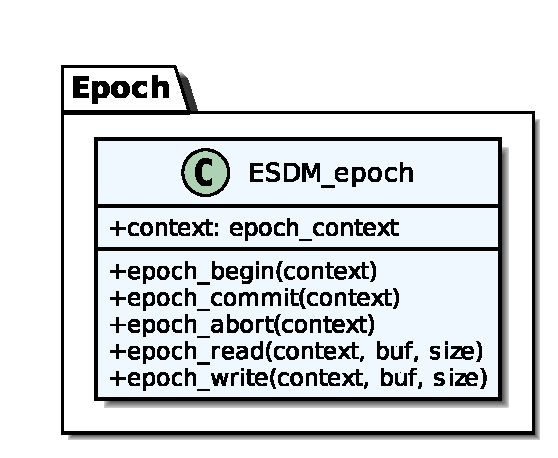
\includegraphics[width=0.38\textwidth]{esdm-semantics/semantics-epoch.eps}
	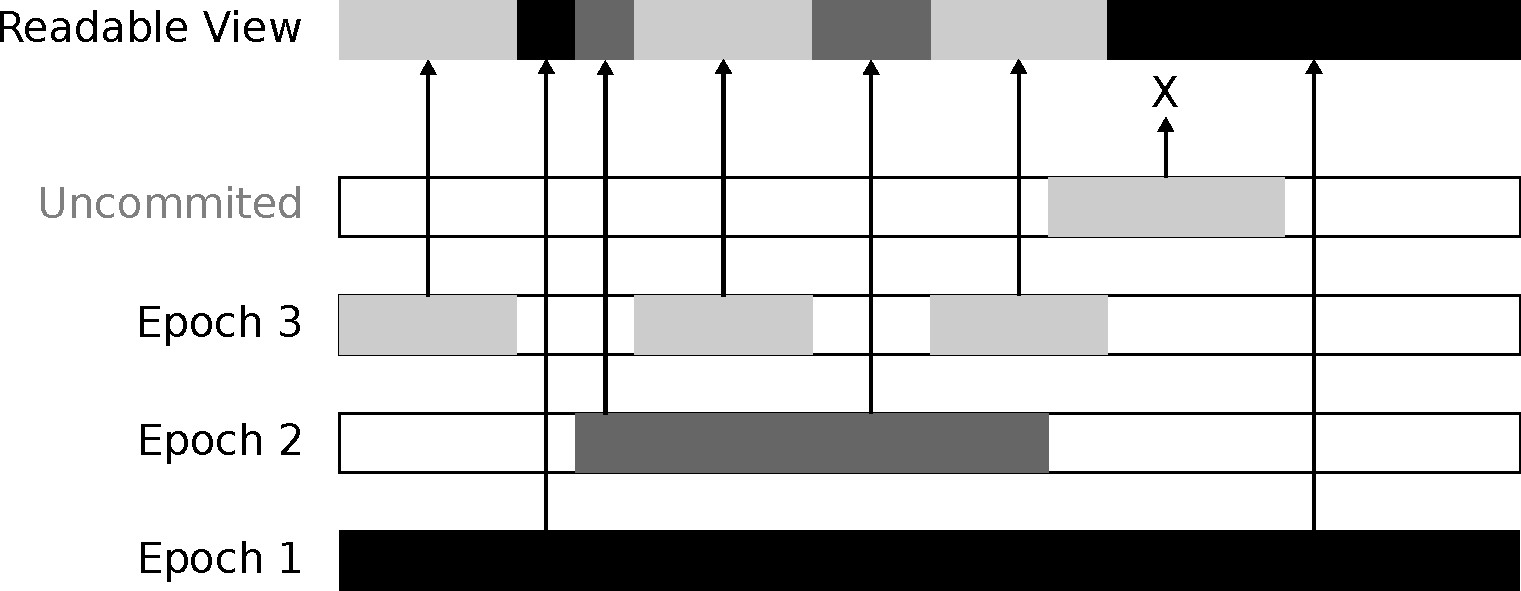
\includegraphics[width=0.6\textwidth]{esdm-semantics/epoch-reconstruction.pdf}
	\caption{Epoch API (left) and the implication of the epoch commit on the reconstruction of the most recent readable view to the data.}
	\label{fig:epoch semantics}
\end{figure}






%%%%%%%%%%%%%
\subsection{Notifications}
\label{sec: viewpoints/logical/data model/notification}

Users or software may register hooks into the ESD notification system watching for certain events to happen.
This is handled as a publish/subscribe service.
Internally, important events are logged and can be queried for the past.
This prevents loss of information in case a service is down for a period of time and ensures auditability.
Tools may use the information to monitor ongoing activity and report performance behaviour of the ESDM.
\Cref{fig:semantic notification} depicts an UML diagram for the interface to ESDM notifications.


\paragraph{Subscribe/Unsubscribe:}
A user or a process that wishes to be informed if a certain event occurs can do so by subscribing to the ESDM Notification system. If notifications are no longer necessary it can also unsubscribe again.

\paragraph{Events:}
ESDM will publish a number of standard events. \Cref{fig:semantic notification} lists a number of candidate event types.

\paragraph{User Events:}
To allow users to define workflows that depend on ESDM, users can register custom named events. Another process that is subscribed to such an event is notified when an event with the name is published.


\paragraph{Event Log:}
To allow for audits and delayed triggering of follow-up tasks in case of failures a event log is kept.
Applications and administrators may use a query interface to filter for events that are relevant.


\begin{figure}
	\centering
	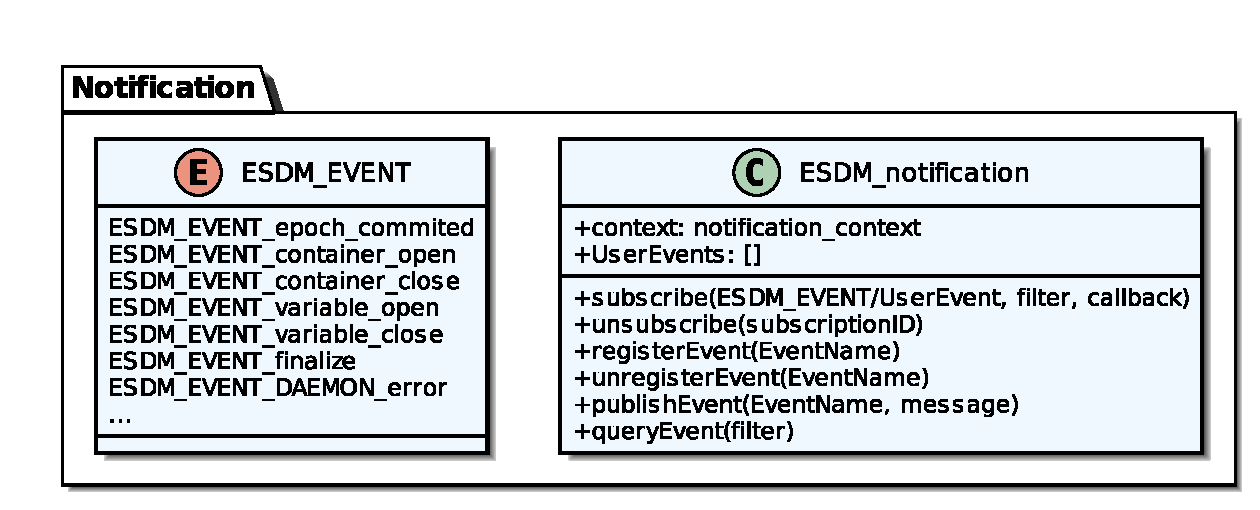
\includegraphics[width=0.8\textwidth]{esdm-semantics/semantics-notification.eps}
	\caption{Notification Interfaces and examples for possible hooks available for subscription. In addition, users may register application specific hooks.}
	\label{fig:semantic notification}
\end{figure}









%%%%%%%%%%%%%%%%%%%%%%%%%%%%%%%%%%%%%%%%%%%%%
\section{Physical view}
\label{sec: viewpoints/physical}

This section describes the relation between ESDM software components and physical hardware components such as  compute nodes, processes and the storage systems.
\Cref{fig:viewpoint physical} illustrates the interactions using UML diagrams.

\paragraph{Applications:} An application process is active on one node and may depend on multiple subcomponents.
Usually, an application will use a library such as NetCDF or HDF5 that provides a portable data description implementation.
With ESDM these libraries are slightly changed to call ESDM to handle I/O for them.
It is possible that multiple processes with ESDM are active on the same node in which case the ESDM should coordinate with processes on the same node.

\paragraph{Daemons:} Besides the application use case, a daemon process maybe necessary to ensure unreferenced fragments are cleaned up and also to perform optimisation without requiring active applications.
Multiple daemons maybe active at the same time.


\paragraph{Storage System:} Multiple storage systems maybe deployed but for the discussion the abstract representation is sufficient.
No changes to the storage backends are expected.
ESDM backends will interact with the storage systems using the interfaces that are exposed by the storage system.

\paragraph{Site Configuration:} The ESDM assumes that there is a description of the site configuration in a machine friendly format. As the system operators change the configuration of the storage systems or the network, the site configuration may need to be updated manually or automatically.




\begin{figure}
	\centering
	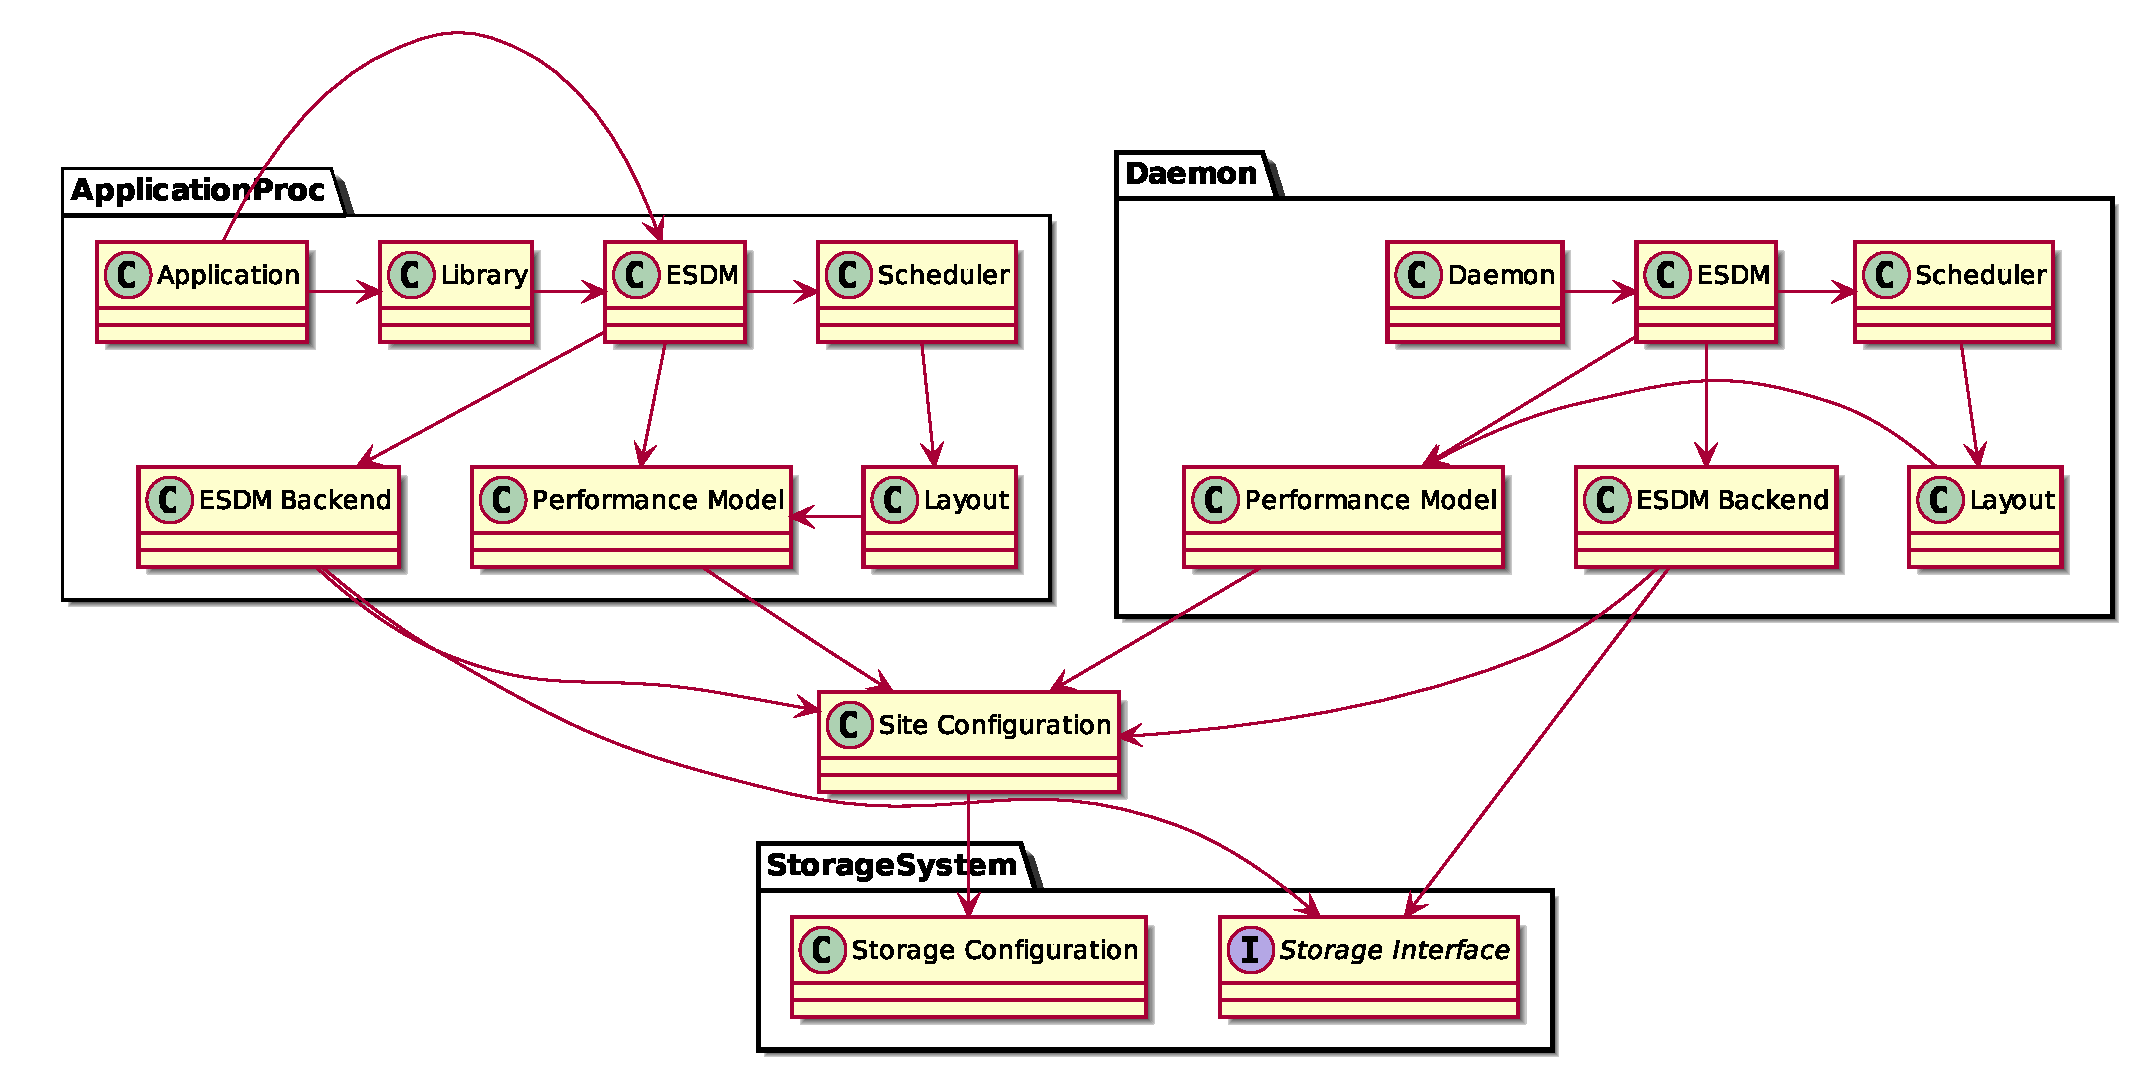
\includegraphics[width=\textwidth]{esdm/physical}
	\caption{Physical viewpoint to the core components of the ESDM.}
	\label{fig:viewpoint physical}
\end{figure}














%%%%%%%%%%%%%%%%%%%%%%%%%%%%%%%%%%%%%%%%%%%%%
\section{Process view}
\label{sec: viewpoints/process}

The process view describes active components and processes of ESDM, their interaction and how they drive the I/O.
The asynchronous I/O calls offered by ESDM still require an internal thread to progress the I/O.
Most components shown in \Cref{fig:architecture} are passive, that means functions invoked perform certain operations and return upon completion.
That means the thread of the application or tool calling ESDM retains inside ESDM until the call is completed.
The FUSE client and potential service daemons are applications in that sense, they bring their own thread that use the API of ESDM.

In the internal architecture of ESDM, the scheduler is the only exception and using threads.
Asynchronous I/O requests from user space are queued as operations to be performed by the scheduler.
% A thread of the scheduler then records the modifications to be made on a write-ahead log  => No not yet! later version
The scheduler may decide upon the order the operations are performed locally.
Internally, the scheduler hosts a queue for each storage backend that are served by a (storage backend-specific) number of threads.
A thread initiates the operation by calling the plugin-specific function.
It is the responsibility of the storage backend to ensure the data is transferred to the respective storage.
An involved storage system above of a capable network may allow RDMA.
In this case, the plugin has to announce the availability of data to the server, then the server may fetch data from the client using RDMA and send a notification upon completion.
Due to the lack of such capabilities on most storage APIs, the capabilities of pulling data is subject to a later version of ESDM.


\paragraph{ESDM daemon}

The ESDM daemon is in charge to constantly check the health of the overall system.
It will remove/garbage collect objects that were created by applications that crashed.
It may start a re-balancing/data migration between the available storage pools based on simple policies.
Also replicas of data may be removed to free space.

% \todo{figure}




\section{Requirements-Matrix}
\label{seq:req matrix}
In this section we re-visit the requirements and show how these requirements are met by some element of the architecture.
Therefore, we list the requirements in \Cref{chap:requirements} in brief and describe how they are addressed by ESDM.

\begin{enumerate}
\item CRUD-operations: The data model provides CRUD operations for the objects and in particular variables that typically hold the scientific data.
\begin{itemize}
\item Partial access: Read/write operations are supported on subdomains for a variable. Internally they may fetch data
from multiple fragments.
\end{itemize}
\item Discover, browse and list data: The ESDM namespace provides a query interface based on scientific metadata.

\item Handling of scientific/structural metadata as first class citizen: Metadata provides similar operations than data.
It can be as complex as a variable, in fact attaching a variable to another as metadata.
Internal components of ESDM are aware of the metadata.
Metadata is used for searching data but also the structural information is directly used by ESDM internally; backends make the final layout decision based on the metadata.

\item Semantical namespace: provided by the metadata queries.
\item Supporting heterogeneous storage: Backends provide plugins to predict performance of access patterns and to store/retrieve data on various storage systems.
A single variable consists of fragments that each cover a subdomain, potentially with another data layout / transformation; each fragment may reside on another backend allowing to distribute a variable across different storage technology.

\item Function shipping: this is not yet described in the design. However, the structural information about the data is a key enabler for function shipping as it allows the storage backend to understand the data structures that may then be processed.

\item Compatibility: we offer a NetCDF and HDF5 interface and a POSIX file system using FUSE.
We will explore the possibility to create data using one interface and accessing the data without data copies using another.
\end{enumerate}



These mandatory requirements are accompanied by supporting requirements:
\begin{enumerate}
\item Auditability: not described in this deliverable.
\item Configurability: ESDM provides the site configuration about available storage systems and their performance characteristics.
\item Notifications: ESDM offers a publish/subscribe interface.
\item Import/Export: This is not explicitly described in this deliverable, but a tool can be build on top of ESDM.
\item Access control: ESDM will use the available access control information but also store the ownership and permissions inside the container.
\begin{itemize}
\item Data sharing: Data sharing is at the moment limited to a site.
However, it would be easy to link a tool that uses the NetCDF interface to ESDM to enable dynamic creation of virtual containers depending on the file name (that is a query for metadata).
\end{itemize}
\end{enumerate}

The non-functional requirements are resolved as follows:
\begin{enumerate}
\item Performant: by moving the serialisation from the application into the backends and by selecting appropriate backends depending on the access patterns using the layout component and the performance model, the system should be able to make superior placement decisions and optimise layout depending on the access pattern.
\item Reliable: Fragments and variables offer methods to check for integrity (e.g., using checksums); ESDM offers replication of data, potentially transformed for performance, thus offers reliable storage.

\item Versatile: By providing a storage backend for a storage technology and a performance model, it can be integrated into ESDM.
\item User-friendly: The system hides specifics of the storage landscape and does not \textit{\textbf{require}} users to set and define technical parameters specifically to a given system.
Therewith it provides performance portable code.
\item Cost-Effective: The software will be open source, it has to be proven that it is cost effective.
\item Standards based: ESDM offers standard interfaces and uses standard interfaces for the backends, making it possible to deploy it on current systems.
\end{enumerate}

%%%%%%%%%%%%%%%%%%%%%%%%%%%%%%%%%%%%%%%%%%%%%
%\section{Development view}
%\label{sec: viewpoints/development}
%\todo{
%* internal interfaces and apis
%* how is Data Models processed internally
%* Abstract: JSON for description of Data Models info, flexible, but certain fields expected => (more details not yet determined, remains to be seen as implementation continues..)
%* How are certain operations of the Data Models implemented for manipulationen of objects within Data Model
%}
%
%




%%%%%%%%%%%%%%%%%%%%%%%%%%%%%%%%%%%%%%%%%%%%%

\chapter{Architecture: Components and Backends}
\label{chap:components and backends}

\begin{chapterIntro}
	This section discusses most relevant components and backends in technical detail.
	For every component listed, the 4+1 view is described (refer to \Cref{sec:about 4+1}).
	The components and backends are ordered according to their position within the I/O stack from top (application) to bottom (backend).

	\Cref{component: scheduler} discusses the scheduling component that breaks down incoming read and write requests into subsequent requests to create or receive multiple fragments.
	The scheduler relies on a layout component to create a set of domain filling subrequests which is discussed in \Cref{component: layout}.
	In most cases, an application will not interface directly with the ESDM middleware but through a common frontend.
	\Cref{frontend: hdf5 + mpi} introduces a HDF5 frontend and also discusses how message passing via MPI is realised outside of the ESDM.
	\Cref{frontend: fuse} addresses legacy interfaces using FUSE to expose data sets via a configurable virtual file systems.

	It follows the discussion of multiple backends.
	In particular \Cref{backend: posix} discusses a POSIX backend to allow for interactions with parallel file systems.
	Object storage backends for Mero (see \Cref{backend: mero}) and WOS (see \Cref{backend: wos}) are discussed,
	Besides data backends, also pure metadata backends are possible allowing to use a existing software stacks that are typically also residing on some kind of storage backend themselves.
	\Cref{backend: mongo} describes MongoDB bases metadata backend.
\end{chapterIntro}



%%%%%%%%%%%%%%%%%%%%%%%%%%%%%%%%%%%%%%%%%%%%%
\section{Scheduling Component}
\label{component: scheduler}


I/O requests handled by the ESD middleware are received via the ESDM interfaces as they are described in \Cref{sec: viewpoints/logical/semantics}.
In most cases, these requests must collect additional information / identify multiple fragments to fulfil a request.
The ESDM scheduler is responsible to progress potentially operations, coordinate requests, and invoke the appropriate handlers.
In particular, the scheduler will consult the layout component to determine which fragments to create or use and which storage backends to use.
For a discussion of the decision process for a mapping of a I/O request to backends refer to \Cref{component: layout} on the layout component.


%%%%%%%%%%%%%%%%%%%%%%%%%%%%%%%%%%%%%%%%%%%%%%
\subsection{Logical View}

\begin{figure}
	\centering
	\includegraphics[width=\linewidth]{esdm-components/scheduler/logical.eps}
	\caption{Logical view to the ESDM scheduling component.
	Applications issue requests that are then handled and delegated by the Scheduler to other components.}
	\label{fig:esdm scheduler logical view}
\end{figure}

The scheduling component has two core responsibilities:

\begin{enumerate}
	\item Accept incoming operations from the ESDM Interface and delegate them to handlers possibly in separate threads.
	\item Coordinate the progressing of complex operations and the response/completion of the operations.
\end{enumerate}

In \Cref{fig:esdm scheduler logical view}, the relation of the scheduling component (scheduler) to the rest of the ESDM architecture is illustrated.
An application will issue a request which is queued to the scheduler for consideration.
The scheduler will delegate the request to the layout component which will also consult a performance model to make a decision (refer to \Cref{component: layout} for details).
The resulting operations to internal objects (fragments) may then require a number of requests to various ESDM backends.
These subsequent operations are also coordinated by the Scheduler.




%%%%%%%%%%%%%%%%%%%%%%%%%%%%%%%%%%%%%%%%%%%%%%
\subsection{Process View}

\begin{figure}
	\centering
	\includegraphics[width=\linewidth]{esdm-components/scheduler/process.eps}
	\caption{Process view to the ESDM scheduling component. Applications should when possible issue I/O asynchronously. In either situation the ESDM scheduler may execute multiple threads in parallel to gather or flush fragments to the backends or make a layout decision.}
	\label{fig:esdm scheduler process view}
\end{figure}

The scheduling component is responsible for the bulk of concurrency within the ESDM.
Requests arrive and have to be dispatched to appropriate handlers such as the layout component or a ESDM backend.
This approach is necessary so the ESDM remains responsive as new requests arrive and because it considerably can speed up the reconstruction/flushing of requested views.
\Cref{fig:esdm scheduler process view} provides a overview to active and waiting process as requests are being handled by the ESDM. Notice that Process 1 handles a asynchronous request which allows the application to continue computation, while Process 2 depicts the synchronous case.
In both cases the ESDM will try to perform the domain reconstruction concurrently.


%%%%%%%%%%%%%%%%%%%%%%%%%%%%%%%%%%%%%%%%%%%%%%
\subsection{Physical View}

\begin{figure}
	\centering
	\includegraphics[width=\linewidth]{esdm-components/scheduler/physical.eps}
	\caption{Physical view to the ESDM scheduling component. The scheduler is only active within the application process.}
	\label{fig:esdm scheduler physical view}
\end{figure}


An application may be spread out across many nodes and on each node have multiple running processes.
Each running process that is using ESDM as a scheduling component running as is illustrated in \Cref{fig:esdm scheduler physical view}.
Within ESDM, only the scheduler starts threads.
The ESDM scheduler does not directly expect any modifications or prerequisites from the storage system, but changes to the configuration of the storage system should be reflected in the site configuration.

%
%%%%%%%%%%%%%%%%%%%%%%%%%%%%%%%%%%%%%%%%%%%%%%%
%\subsection{Development View}
%
%\begin{figure}
%	\centering
%	\includegraphics[width=\linewidth]{esdm-component/scheduler/development.eps}
%	\caption{}
%	\label{fig:esdm scheduler development view}
%\end{figure}
%
%\Cref{fig:esdm scheduler development view}
%
%


%%%%%%%%%%%%%%%%%%%%%%%%%%%%%%%%%%%%%%%%%%%%%
\clearpage
\section{Layout Component}
\label{component: layout}

The layout component is responsible for finding a mapping to storage that takes into account information that are available through the conceptional and logical views to the data.
In addition, this section addresses some aspects that explain how the mapping is driven by performance models and the site configuration.


%%%%%%%%%%%%%%%%%%%%%%%%%%%%%%%%%%%%%%%%%%%%%%
\subsection{Logical View}

\begin{figure}
	\centering
	\includegraphics[width=\linewidth]{esdm-components/layout/logical.eps}
	\caption{An application that is using ESDM interfaces through the ESDM API (which in many cases maybe only read/write calls). Eventually the scheduling component has to consult the layout component which is responsible for returning a list of Fragments which have to be read or written. To provide this list the performance model is used which in turn queries the available backends and the site configuration for an estimate.}
	\label{fig:esdm layout logical view}
\end{figure}

The layout component is invoked by the ESDM scheduler to break down incoming requests into fragments that are beneficial from a data access and storage perspective.
The layout components responsibilities in more detail include the following:

\begin{itemize}
	\item map (e.g., a domain) to fragments
	\item where to save new/additional/replica fragments?
	\item time estimates for reading a fragment (e.g., a callback per backend and configuration provided)
	\item time estimates for writing a fragment, in particular find a domain mapping
\end{itemize}

\Cref{fig:esdm layout logical view} illustrates the embedding of the layout component into the larger ESDM architecture.
To find a mapping an important factor is the performance of the individual backends, which requires to know which backends are available.
\Cref{sec:layout/logical/init} describes the initialization process that loads the site configuration.
Storage backends feature wildly different performance characteristics, which is why the ESDM features an abstract performance model that queries the individual ESDM backends to provide performance estimates which may also depend on the data structure of the request.
\Cref{sec: layout/logical/decision} describes the performance model and decision process in more detail.

\subsubsection{Initialization of the Layout/Performance Model}
\label{sec:layout/logical/init}

The layout decision requires knowledge of the available backends.
The ESDM assumes a machine-friendly site configuration to be available.
The site configuration includes a list of available backends for which the ESDM on initialization loads.
\Cref{fig:esdm layout initialisation} shows a UML sequence diagram of the ESDM initialisation process.

\begin{enumerate}
	\item Application/Library: calls ESDM initialisation
	\item ESDM:
	\begin{enumerate}
		\item reads configuration file
		\item discovers and loads available backends + plugins + backend performance model
		\item available backends are announced to the ESDM performance model for consideration
	\end{enumerate}
	\item After successful initialization control is returned to the calling application/library.
\end{enumerate}

\begin{figure}
	\centering
	\includegraphics[width=\linewidth]{esdm-components/layout/sequence_init.eps}
	\caption{The initialisation process of the ESDM and the performance model and also the available backends.}
	\label{fig:esdm layout initialisation}
\end{figure}



\subsubsection{Performance Model and Decision Process}
\label{sec: layout/logical/decision}

One approach to find the best backend/backends is to query every backend for a performance estimate and choose the most affordable.
\Cref{fig:esdm layout choose backend} shows in a simplified example how the decision process for a data center with three storage systems may look like.
The decision would gather estimates by calling the performance model (PM) of every backend.
Performance metrics may include:

\begin{itemize}
	\item Latency
	\item Throughput (read/write)
	\item Energy/Cost
	\item Capacity/Fill level
\end{itemize}

Users or administrators may weight which factors are most important for their application.
The decision process has to be configurable because different sites have different requirements.

\begin{figure}
	\centering
	\includegraphics[width=0.5\linewidth]{esdm-components/layout/performance-model.pdf}
	\caption{A layout decision component queries the performance estimates for every backend and also takes the domain into account. Possibly other metrics such as the available capacity for every backend may as well be considered.}
	\label{fig:esdm layout choose backend}
\end{figure}

% Unadressed: When to release allocated memory?


\subsubsection{Layout Reconstruction}

When applications are reading data the ESDM Scheduler consults the layout component for a domain reconstruction.
A subdomain description is passed to the layout component as part of request.
The layout component then requests metadata for the container/variable to be received.
From the list of available fragments the layout component has now to choose a subset of fragments that can be read efficiently from the backends.
To decide which fragments to choose the performance model is consulted.


%%%%%%%%%%%%%%%%%%%%%%%%%%%%%%%%%%%%%%%%%%%%%%
\subsection{Process View}

For the layout component to types of processes can be distinguished:

\begin{itemize}
	\item Layout reconstructions and finding fragmentation
	\item Gathering performance estimates
\end{itemize}

\Cref{fig:esdm layout process view} illustrates the possible process in am UML diagram.
Layout reconstructions may result in multiple requests to multiple ESDM backends.
How ESDM gathers/flushes these fragments concurrently is described in \Cref{component: scheduler}.


\begin{figure}
	\centering
	\includegraphics[width=\linewidth]{esdm-components/layout/process.eps}
	\caption{Multiple process are involved with most applications. For every node the performance decisions maybe different, but in many cases it also maybe desirable to find an estimate collectively. Ultimately the performance estimate needs to be relatively cheap to compute. }
	\label{fig:esdm layout process view}
\end{figure}





%%%%%%%%%%%%%%%%%%%%%%%%%%%%%%%%%%%%%%%%%%%%%%
\subsection{Physical View}

\begin{figure}
	\centering
	\includegraphics[width=\linewidth]{esdm-components/layout/physical.eps}
	\caption{Physical view for the layout component a closely related components.}
	\label{fig:esdm layout  physical view}
\end{figure}

The layout component relies on multiple subcomponents, all of which only exist within the application process.
\Cref{fig:esdm layout physical view} illustrates the distribution and relation of the components across different hardware components.
The site configuration is expected to be pulled from a storage system that can withstand a large number of reading clients.
Nodes may cache the site configuration locally.
The ESDM layout component does require prerequisites from the storage system, but changes to the configuration of the storage system should be reflected in the site configuration.


%%%%%%%%%%%%%%%%%%%%%%%%%%%%%%%%%%%%%%%%%%%%%%%
%\subsection{Development View}
%
%\begin{figure}
%	\centering
%	\includegraphics[width=\linewidth]{esdm-layout/development.eps}
%	\caption{}
%	\label{fig:esdm layout development view}
%\end{figure}




%%%%%%%%%%%%%%%%%%%%%%%%%%%%%%%%%%%%%%%%%%%%%
\clearpage
\section{HDF5+MPI plugin}
\label{frontend: hdf5 + mpi}
This section describes the implications on an existing parallel application that uses one of the supported interfaces such as NetCDF4/HDF5.
The semantics of the API calls will change slightly but typically in a way that is backwards compatible.

\subsection{Logical View}


\begin{figure}
	\centering
	\includegraphics[width=\linewidth]{esdm-hdf5+mpi/logical.eps}
	\caption{Logical view to the HDF+MPI plugin.}
	\label{fig:esdm hdf5 logical view}
\end{figure}

This subsection covers dealing with file names, opening and closing of containers as well as concurrency semantics.
We assume an MPI parallelized application uses HDF5 with MPI support, e.g., parallel HDF5.
The component diagram in \Cref{fig:esdm hdf5 logical view} illustrates how a HDF5/NetCDF ESDM frontend would mediate between the ESDM and an application.
In addition, multiple processes using ESDM can coordinate using MPI, though only ESDM component using MPI is the ESDM HDF5 VOL Plugin.




\subsubsection{Dealing with file names}

Traditionally, when opening a file with NetCDF the filename specifies the location, i.e., a URI where the data resides on a storage system.
We change the notion of the file name to be the descriptor for a virtual container (virtual container descriptor).
The virtual container can be composed of multiple URIs to integrate different variables into one virtual environment on the fly.
Thus, from the reader's perspective it does not matter if data of a model is split into one or multiple physical files; upon read, all those files can be loaded together as if they would already exist in one logical file.
It is also possible to avoid the use of the metadata backend; by specifying the locations of the variables on existing storage media, they can be linked into a virtual container.
One restriction to this approach is the limitation of the length of file names.
To avoid this limitation, we support a prefix to the filename: \texttt{esd-cfg:/} that leads to a simple JSON file that contains the actual definition of the container.

\subsubsection{Open}

Opening a container (as defined by the file name) in ESDM will trigger the master process within the communicator to retrieve the necessary metadata from ESDM and broadcast it to all participating processes.
Since the metadata is serializable to JSON, we can exchange the metadata easily.

\subsubsection{Concurrency semantics}

In general, the system is designed for parallel applications of which processes access data independently of each other.
Still, metadata of internal objects such as containers and variables should be managed and updated explicitly by a single process of the application.
That means, within one parallel (MPI) application, some kind of coordination must take place to allow the shared access to containers, variables and shards.
A correct implementation for this behavior will be performed within the HDF5 VOL plugin.

Data sharing between independent applications is intended to happen after an epoch has been completed.
It is not allowed that multiple parallel applications write data to the same variable at the same time.
This is considered to be sufficient for most scenarios, e.g., a model produces some output; once the epoch  completed, the produced data is post-processed.

\subsubsection{Close}

From the user perspective, closing a file that was opened in write mode, will make the content of the file visible in ESDM and durable for subsequent accesses.
Thus, it updates the metadata, for example, incrementing the epoch of the variables and containers modified and updating the reference counters.

\subsection{Physical View}


\begin{figure}
	\centering
	\includegraphics[width=\linewidth]{esdm-hdf5+mpi/physical.eps}
	\caption{Physical view to the HDF5+MPI plugin.}
	\label{fig:esdm hdf5 physical view}
\end{figure}

ESDM does not change anything of the placement of the processes run by MPI.
\Cref{fig:esdm hdf5 physical view} illustrates the distribution and relation of the components across different hardware components.


\subsection{Process View}

\begin{figure}
	\centering
	\includegraphics[width=\linewidth]{esdm-hdf5+mpi/process.eps}
	\caption{Process view to the HDF5+MPI plugin.}
	\label{fig:esdm hdf5 process view}
\end{figure}

ESDM will start internally threads in the Scheduler component, however, these threads will not call MPI functions or HDF5.
The ESDM plugin in the HDF5 VOL may use MPI functions (or the lightweight library) to coordinate access to central data structures.
\Cref{fig:esdm hdf5 process view} illustrates the process view as far as the HDF5 VOL plugin and MPI coordination is concerned.



%%%%%%%%%%%%%%%%%%%%%%%%%%%%%%%%%%%%%%%%%%%%%
\clearpage
\section{Fuse Legacy + Metadata Mapped Views}
\label{frontend: fuse}

Filesystem in Userspace (FUSE) provides a relatively simple means to export a view to data as a virtual file system, but without the need for special privileges associated with similar techniques. FUSE is thus a popular choice to achieve legacy support for applications that require POSIX-like access semantics.


%%%%%%%%%%%%%%%%%%%%%%%%%%%%%%%%%%%%%%%%%%%%%%
\subsection{Logical View}

\begin{figure}
	\centering
	\includegraphics[width=0.5\linewidth]{esdm-fuse/logical.eps}
	\caption{Based on a FUSE ESDM configuration different views to data are possible. HDF5 files maybe created as soon as a job is known or on the fly.}
	\label{fig:esdm fuse logical view}
\end{figure}

Compatibility to legacy applications is the main motivation to provide a ESDM FUSE  file system.
Allowing different views to the same data based on the available metadata information is another motivation.
Examples for  metadata mappings to a hierarchical namespace could be as follows:

\begin{itemize}
	\item  \texttt{modelname/date/variable.h5}
	\item  \texttt{region/date/modelname/variable.nc}
\end{itemize}

The structure of the hierarchy could be up to the users.
The limit at this point would be the quality of available metadata as it is in already existing metadata catalogues.
\Cref{fig:esdm fuse logical view} illustrates how the ESDM FUSE file system would be used by a scientist.
In an ideal setting, the ESDM has some time to analyse e.g. a submitted job script to figure out which HDF5 will be requested.
The ESDM would then use the HDF5 creator to generate the HDF5 files before the job is started/beginning to read from the file.
After the ESDM HDF5 creator has created the file, the ESDM FUSE would read and write from this file.
If a generated it not used for a while, it may be removed again to make room for more recent requests.


\paragraph{Access Semantics:}
HDF5 files usually allow to be modified to add metadata or update variables and data sets.
The ESDM legacy interface likely will be read only.
A possible update of the original ESDM data structures to reflect changes made to the HDF5 view is not planned, to avoid potential consistency conflicts.
The structure of the HDF5 and the directory structure of available files depends on a ESDM FUSE configuration.



%%%%%%%%%%%%%%%%%%%%%%%%%%%%%%%%%%%%%%%%%%%%%%
\subsection{Development View}
\label{sec: fuse/development}

%
%\begin{figure}
%	\centering
% 	\includegraphics[width=0.5\linewidth]{esdm-fuse/development.eps}
%	\caption{}
%	\label{fig:esdm layout development view}
%\end{figure}


Some applications may not be compatible to HDF5 with virtual object layer (VOL).
For such application it is necessary to export data stored within ESDM as actual HDF5 files.
A FUSE interface allows to automate the export without requiring to generate the actual HDF5 files unless they are requested.
Two approaches for exposing HDF5 files are:

\begin{itemize}
	\item Recreate sections of HDF5/NetCDF files, as they are being read, on the fly. Potentially very complicated, especially for read and write. This is not very desirable from a performance perspective. Refer to \url{https://support.hdfgroup.org/HDF5/doc/H5.format.html} for file format details.
	\item Write a brand new HDF5 file based on the requested data/query.
\end{itemize}

While it maybe in possible to fulfil requests to virtual HDF5 files without generating the actual file, the architecture of HDF5 with different file format drivers leads and HDF5 internal caching makes such an approach unfeasible.


\subsubsection{Use HDF5 to create file on the fly}

The ESDM FUSE interface for HDF5 files should act as a cache layer for HDF5 exports generated on demand, while allowing
to browser available data sets and variables from a file system.
\Cref{fig:fuse hdf5 sequence} illustrates this process in a UML sequence diagram.
A legacy application makes a request to the FUSE file system, which is handled by the ESDM middleware that will use HDF5 to create a HDF5 file.


\begin{figure}
	\centering
	\includegraphics[width=\linewidth]{esdm-fuse/sequence.eps}
	\caption{The simplest approach to expose data to legacy applications by creating actual HDF5 files on the fly and cache them on a file system.}
	\label{fig:fuse hdf5 sequence}
\end{figure}



%%%%%%%%%%%%%%%%%%%%%%%%%%%%%%%%%%%%%%%%%%%%%%
\subsection{Process View}


\begin{figure}
	\centering
	\includegraphics[width=\linewidth]{esdm-fuse/process.eps}
	\caption{Process view to a FUSE legacy backend for ESDM. An application browsers a FUSE file systems which is generated based on the available metadata. As the application opens a file, the ESDM creates a HDF5 file which can be then read just a usual HDF5 file.}
	\label{fig:esdm fuse process view}
\end{figure}

Following the reasoning in \Cref{sec: fuse/development} HDF5 files would need be generated and stored before file access requests can be handled.
\Cref{fig:esdm fuse process view} separates the process of accessing a available file and the actual generation of the file.
If the application is already running and the requests HDF5 file is not already present, the reconstruction can be performed on the node of the application.
If the application is not yet running, the scheduler could start a reconstruction before the application is started.
In both cases a component that generates the HDF5 file is required which is represented by the ESDM HDF5 Creator.







%%%%%%%%%%%%%%%%%%%%%%%%%%%%%%%%%%%%%%%%%%%%%%
\subsection{Physical View}

\begin{figure}
	\centering
	\includegraphics[width=\linewidth]{esdm-fuse/physical.eps}
	\caption{Physical View: Allow legacy applications to access data stored to ESDM by creating HDF5 on the fly or by scanning job files in advance.}
	\label{fig:esdm fuse physical view}
\end{figure}

The provision of a FUSE legacy interface allows for a number different deployment models.
\Cref{fig:esdm fuse physical view} illustrates where the ESDM FUSE related component would be active within the data centre.
To require only little modifications and exploit independent data access FUSE is assumed to be available on the compute nodes.
The scheduler may be modified to start the ESDM HDF5 Creators before spawning a job.
The actual ESDM data as well as temporary HDF5 files would be stored and distributed across multiple storage systems.




%%%%%%%%%%%%%%%%%%%%%%%%%%%%%%%%%%%%%%%%%%%%%
\clearpage
\section{Backend POSIX/Lustre (Using ESDM)}
\label{backend: posix}

Most climate applications today read and write from and to parallel file systems such as Lustre.
The section describes how a POSIX-like backend to the ESDM would handle read and write requests and organise the ESDM data structures.


%%%%%%%%%%%%%%%%%%%%%%%%%%%%%%%%%%%%%%%%%%%%%%
\subsection{Logical View}
\label{backend: posix/logical}

\begin{figure}
	\centering
	\includegraphics[width=\linewidth]{esdm-backends/POSIX/logical.eps}
	\caption{Logical view to the POSIX backend. I/O requests arrive through the ESDM API. The layout component provides a fragmentation (write: site config + perf model / read: as stored in metadata + optimisation candidate). As a result, actual I/O requests are processed by the progress component which calls the backends. The backends and the datatype components work together to convert data according to what is required (read and write differ).}
	\label{fig:backend posix logical view}
\end{figure}

In the previous sections, we have discussed how the scheduler (see \Cref{component: scheduler}) accepts requests by applications and libraries and then consults the layout component (\Cref{component: layout}) to decide on a layout.
In this section, we assume the POSIX backend was chosen.
\Cref{fig:backend posix logical view} illustrates the associated components and which components interact with each other.
Requests made to the POSIX backend can be classified into one of three types.
On the one hand, there are read and write requests to the data.
In addition, there may be metadata lookup, which will in most cases relate to technical metadata.
The following paragraphs explain each of these access types in more detail.


\paragraph{Writing data}
To satisfy write requests, this section extends the use-case description for general writing (see \Cref{uc: independent write}).
The sequence of events relevant to the POSIX backend (also illustrated in \Cref{fig:backend posix sequence write}) unfolds as follows:

\begin{enumerate}
	\item Progress: consults layout about:
	\begin{itemize}
		\item Which Backend?
		\item Which Fragmentation?
	\end{itemize}
	\item Scheduler: processes write calls for all fragments and hands data to POSIX backend
	\item Layout: decides for the specific backend that is suitable for the individual fragment (e.g. row-way serialisation)
	\item Backend: converts between file serialisation and ESDM datatypes
\end{enumerate}

For a POSIX backend, many potential mappings to files and directories are possible.
Which mappings are the most efficient is an open research question and depends on the application.
A straight forward approach is to use the directory structure to map hierarchical concepts, e.g. from NetCDF or HDF5 such as groups and data sets.
The files within the data set directory would include a description of the domain and an additional directory that is used to store the actual fragments.

\begin{figure}
	\centering
	\includegraphics[width=\linewidth]{esdm-backends/POSIX/sequence_write.eps}
	\caption{Sequence Diagram for writes to the POSIX Backend.}
	\label{fig:backend posix sequence write}
\end{figure}



%%%%%%%%%%%%%%%%%%%%%%%%%%%%%%%%%%%%%%%%%%%%%%%%
\paragraph{Reading data}

Analogue to the write case, the reading data with a backend extends the use-case description for general reading (see \Cref{uc: independent read}).
The sequence of events relevant to the POSIX backend (also illustrated in \Cref{fig:backend posix sequence read}) unfolds as follows:

\begin{itemize}
	\item Read arrives
	\item Progress receives requests and splits it potentially into multiple subrequests
	\item Layout loads metadata, consults indexes and collects a sufficient amount of fragments to reconstruct requested (sub)domain in parallel and from the most ``affordable'' backends
	\item Progress (potentially coordinated across multiple processes) issues requests to backends
	\item Backends fetch data and return Fragments
	\item Backend + Layout + Datatype perform necessary conversations
	\item Data is provided to the application
\end{itemize}



\begin{figure}
	\centering
	\includegraphics[width=\linewidth]{esdm-backends/POSIX/sequence_read.eps}
	\caption{Sequence diagram for reads to the POSIX backend.}
	\label{fig:backend posix sequence read}
\end{figure}



\paragraph{Lookup:}

\Cref{sec: viewpoints/logical/data model} introduced the ESDM data model.
A backend is responsible for storing a fragment and finding the fragment again when it is requested.
The POSIX backend will use indexes to allow for a fast search for required fragments.
In addition, fragments are written in sequence from a linked list that allows reconstructing either the domain or the index in case an index is damaged.
Fragments metadata should allow for partial access of fragment.
To allow this a POSIX Fragment wraps the ESDM fragment to attach technical metadata relevant only for the POSIX backend.
A UML diagram illustrating the relationship between POSIX Fragments and ESDM fragments is depicted in \Cref{fig:backend posix fragment}.

\begin{figure}
	\centering
	\includegraphics[width=0.5\linewidth]{esdm-backends/POSIX/fragment.eps}
	\caption{The ESDM Fragment features a Metadata section that describes the position within a domain. The actual data is simply a blob. Backends are free to extend ESDM Fragments to their liking.}
	\label{fig:backend posix fragment}
\end{figure}





%%%%%%%%%%%%%%%%%%%%%%%%%%%%%%%%%%%%%%%%%%%%%%
\subsection{Process View}
\label{backend: posix/process}

\begin{figure}
	\centering
	\includegraphics[width=\linewidth]{esdm-backends/POSIX/process.eps}
	\caption{Overview of processes that are necessary or interact/interfere with the POSIX backend.}
	\label{fig:backend posix process view}
\end{figure}

\Cref{fig:backend posix process view} illustrates the process view for the POSIX backend. In addition, interactions between the following services and processes are relevant:


\paragraph{Scheduler component}
The progress component is responsible for handling any sync calls as well as outstanding async calls that have to be passed to the backend.


\paragraph{ESDM Compactor component}
The ESDM compactor may either reorganise POSIX data snippets on their on.. e.g. when running as a daemon that improves and maintains the system health.
As applications issue I/O the progress component may use the ESDM compactor when the decision component determines feasible reorganisation/compactification.


\paragraph{(Competing Load):}
Other resources may access the same storage backend or even the same data.
For example, workflows may compete for access to the same storage target which may influence the decisions used for compactification.


\paragraph{(Service Loads):}
The backends usually employ service workloads that ensure system health.
%How do ESDM and their workloads interfere with each other?




%%%%%%%%%%%%%%%%%%%%%%%%%%%%%%%%%%%%%%%%%%%%%%
\subsection{Physical View}

Active software components related to the ESDM that are involved in handling requests are spread across the application process and when they are finally written on the POSIX storage system as illustrated in \Cref{fig:backend posix physical view}.
No changes to POSIX are assumed, but a POSIX backend will call the interfaces these storage systems expose.

Notice that POSIX in this graphic provides a performance model, which is technically not the case for the current ESDM because the system runtime information such as fill level is not communicated actively by the storage system but are instead collected by, e.g., the ESDM POSIX Backend Plugin.


\begin{figure}
	\centering
	\includegraphics[width=\linewidth]{esdm-backends/POSIX/physical.eps}
	\caption{Physical mapping of components to location of their execution?}
	\label{fig:backend posix physical view}
\end{figure}



%%%%%%%%%%%%%%%%%%%%%%%%%%%%%%%%%%%%%%%%%%%%%%%
%\section{PFS Backend}
%
%\todo{Relocate into Architecture Section?}
%\todo{Probably multiple such use cases to describe the backends.}
%
%Storage entities: files, directories
%
%Permissions:
%* Mapping description
%
%Mapping from containers, variables and fragments:
%A fragment is a file:
%* data
%* support structures (index)
%
%Epoch
%*
%
%
%General description of PFS backend. Motivated by use cases.
%
%



\section{Mongo DB Metadata backend}
\label{backend: mongo}

A prototypical metadata backend will be realised using MongoDB.
Advantages of using MongoDB are that it scales horizontally with the number of servers, provides fault-tolerance and that the document model supports arbitrary schemas.


Each type of object in the data model (container, variable, fragment) becomes a collection with indices on certain fields.
Multikey indices allows indexing array fields such as the references.



\subsection{Logical View}
\label{backend: mongo/logical}

\subsubsection{Metadata}

There are two methods to include metadata, large metadata is includes as a reference to another variable containing the data, small metadata is embedded into the JSON of the MongoDB document.

Besides scientific metadata, the dynamic mapping of data to storage backends requires further metadata that must be managed.
To distinguish technical metadata from scientific metadata, an internal namespace is created.
Relevant technical metadata is shown in \Cref{tbl:additionalTechnicalMetadata} for shards, variables and containers, respectively.

Metadata can be optional (O) or mandatory (M), and either is created automatically or must be set manually via the APIs.
Automatic fields cannot be changed by the user.
Some of the data can be automatically inferred, if not set manually, but manual setting may allow further optimisations.

Some of the metadata is used on several places, for example, information about the data lineage might be used to create several output variables.
In our initial implementation, the metadata is stored redundantly because it
1) simplifies search; 2) enables us to restore data on corrupted storage systems by reading the metadata; 3) reduces contention and potentially false sharing of metadata.
An implementation might decide to reduce this by utilising normalised schemas.

References are the list of objects that are directly used by this object, e.g., other variables that are used to define the data further.

\begin{table}
	\begin{subtable}[t]{\textwidth}
		\begin{tabular}{llll}
			Metadata & Field & Creation & Description\\
			\hline
			Domain   & M & Auto & The subdomain this data covers from the variable\\
			Type     & M & Auto & The (potentially derived) datatype of this shard\\
			Variable & M & Auto & The ID of the varitechnical-on-metadata.texable this data belongs to\\
			Storage  & M & Auto & The storage backend used and its options\\
			References & M & Auto & A list of objects that are referenced by this data\\
			Sealed   & M & Auto & A sealed shard is read-only\\
		\end{tabular}
		\caption{For a shard}
	\end{subtable}

	\begin{subtable}[t]{\textwidth}
		\begin{tabular}{llll}
			Metadata & Field & Creation & Description\\
			\hline
			Domain      & M & Manual & Describes the overall domain\\
			Type   	    & M & Manual & The (potentially derived) datatype\\
			Info   	    & M & Manual & The scientific metadata of this document\\
			References  & M & Auto & A list of objects that are referenced by this data\\
			Permissions & M & Auto/Manual & The owner and permissions \\
			Shards      & M & Auto & The list of shard objects for this variable\\
			Sealed      & M & Auto & A sealed variable is read-only\\
		\end{tabular}
		\caption{For a variable}
	\end{subtable}


	\begin{subtable}[t]{\textwidth}
		\begin{tabular}{llll}
			Metadata & Field & Creation & Description\\
			\hline
			Owner    & O     & Manual   & The owner of this file view (see the permission model)\\
			Info     & O     & Manual   & Additional scientific metadata for this view\\
			Directory & O    & Manual   & Contains a mapping from names to variables\\
			Environment & O  & Automatic & Information about the application run\\
			Permissions & M & Auto/Manual & The owner and permissions \\
			References  & M & Auto & A list of objects that are referenced by this data.
		\end{tabular}
		\caption{For a container}
	\end{subtable}
	\caption{Excerpt of additional technical metadata}
	\label{tbl:additionalTechnicalMetadata}
\end{table}



%\subsection{Metadata mapping: Needs updating}
%\todo{Some examples driven from the use cases}
%

%%%%%%%%%%%%%%%%%%%%%%%%%%%%%%%%%%%%%%%%%%%%%%%%%%%%%%%%%%%%%%%%%%%%%%%%%%%%%%%
\subsubsection{Adaptive Data Mappings}
The typical storage mapping for scientific data format libraries is the file (linear sequence of bytes organized following the POSIX file system representation, i.e. inodes and blocks). Information is translated into a linear array of bytes in the file system using appropriate schemas. Since the data model defined by the data format library can contain complex hierarchies and attributes besides raw data, the final file will contain additional scientific metadata that needs to be accessed using the POSIX-IO data interface (e.g. \texttt{read()} and \texttt{write()}) instead of the file metadata interface (e.g. \texttt{stat()}, \texttt{lookup()}). This makes the storage model adopted by data format libraries incompatible with the typical parallel file system organization, in which metadata and data are splitted apart and assigned to different services for optimal performance. Additionally, new storage system paradigms have emerged in the last years in which files are organized in a flat namespace (e.g. object storage), removing the restrictions imposed by metadata operations like namespace traversal of POSIX file systems. Hierarchical organization can be still achieved using other dedicated storage representations like key-value stores, at the expense of reduced POSIX semantic.

There is therefore a necessity for more flexible data mappings that can take advantage of an increasing number of storage and backend alternatives, improving access efficiency at the same time. There are two different approaches to this problem: the first is to develop a new data mapping schema for every storage backend. This is the solution adopted by the HDF5 library (through the virtual file and the virtual object layers) in which multiple storage backends can be employed by developing a corresponding plugin that contains the right mapping schema. The obvious limitation of this solution is that once the user has selected a certain backend for a file, this cannot be changed without migrating the whole file to another backend. The second approach is more flexible and consists in making the storage backend selection adaptive. This has the advantage of enabling backend storage selection on the fly depending upon the type of data being stored or a set of user/system defined parameters (e.g. list of data placement policies satisfying certain requirements of quality of service).

Our proposed solution is to integrate the adaptive data mappings capabilities just discussed in the layout component of the ESD middleware. The middleware will understand the scientific metadata of other relevant data format libraries and will be able to use multiple storage backends at the same time to store and retrieve different pieces of data. To support multiple formats the datatype component in the ESD middleware will expose a datatype interface similar to the one available in HDF5 (described in Section~\ref{sec: data-formats}). Additionally, the middleware will add significant metadata to be used in the life cycle management and sharing of data. This can include semantic metadata describing which data is needed and how it is going to be used, the required level of resilience, etc. In this context, some metadata can be automatically generated by the middleware or defined by the user and passed to the middleware through an apposite interface (that will be part of the ESD exposed interface).

Legacy codes will have access to data using a familiar POSIX interface exported through an ESD FUSE module. The FUSE module will communicate with the ESD middleware to access data and export it to users using a namespace representation. The mapping schema definition for mapping data between the storage representation and the namespace will be done later in the project.

Another important aspect to consider when talking about adaptive data mappings is the storage tiering, that is, how many levels of storage there are in the system. Historically, HPC applications have relied on parallel file systems as first tier to store and retrieve their data. Besides the parallel file system, most high-end clusters have a second level of archival storage to which data is migrated from the parallel file system using a hierarchical storage manager. Nowadays compute nodes have access to local storage (typically a block device formatted with a local file system) and with the emergence of new storage technologies, such as non-volatile memories, permanent byte addressable memory. The ESD middleware should be able to exploit these local storage resources to implement prefetching strategies (read patterns) and burst buffers (write patterns).

%In the specific case of Mero (Seagate object store system), which represents one of the possible storage backends that has to be supported by the ESD middleware, hierarchical and semantic metadata can be stored in the key-value store service while array data can be stored into objects. In fact, we can think about using more than one object per dataset. This is particularly useful with chunking since every chunk in the dataset can be mapped to a different object, making parallel access to different data units possible without any need for I/O coordination (no false sharing is possible in this case). Of course, I/O coordination still needs to be provided when multiple processes access the same dataset and chunking is not enabled. In this case the ROMIO library already provides a collective I/O implementation that can be reused by the ESD middleware. Whenever needed, false sharing of data can also be avoided by using `persistent file realm' like mechanisms\footnote{This mechanism allows a certain file portion to be assigned to a specific process in the application and makes this assignment persistent across multiple data accesses.}.

%\todo{Giuseppe: you had a very good document on this already can add something here}

%Goal of the dynamic mapping is to create a hierarchical namespace based on the available metadata.
%It is based on the search for objects.
%With the help of FUSE, these mappings can be created based on a user configuration upon mount-time (supports user mounts).
%Inaccessible data, i.e., where the permissions are not sufficient, can be hidden from the namespace.

%An example mapping could be:
%“v.info.model/v.info.environment.date/v.info.experiment.tags/v.info.name <as NC4>”.
%This would show a single NetCDF4 file for each variable.
%If a variable is attached to various tags, then it is shown for each of them.

%“v.info.model/v.info.environment.date/v.domain.time/v.info.name <as NC4>”.
%Would show one file per timestep.

%How to resolve ambiguity?

%Existing containers can also be directly mapped, showing the input and output variables similarly:
%“<c.\_id>/<c.directory>”


%The storage should now how the logical data space maps to physical positions in memory or storage.
%If the storage backends have this knowlege, they can run local operations on the data.

%Alternatives:
%Triangular grid (locally refined), somehow mapped from user-space to a 1D structure which gets mapped to the storage. (Traditional approach)

%Application(data structure) - Mapping - Middleware - Mapping (byte array) - Storage API - Storage backend

%or:

%Application - Middleware - Storage API - Mapping - Storage backend

%Use sth. like MPI datatypes to descripe memory (in the application)
%Add metadata to describe the meaning / semantics, additional gain: resilience because we know which data to replicate to put into triple ECC ...
%Add hints how the data is used / will the used in the future

%Avoid redundant descriptions of memory / storage.
%Users stores a 3D field, it is clear which storage location is responsible for [x,y,z]
%How to store triangles etc.

%Why not store code as description?
%- describes neighborhood?

%Coordinates? Universal coordinates, application coordinates?

%VTK? haben diverse Datenstrukturen hierfÃŒr.


%Separation of concerns...

%Missmatch of Chunks size and application domain

%false sharing

%Pointer Datentyp: strong ptr, weak ptr.
%like Boost usw.


%NVRAM



%%%%%%%%%%%%%%%%%%%%%%%%%%%%%%%%%%%%%%%%%%%%%%%%%%%%%%%%%%%%%%%%%%%%%%%%%%%%%%%
\subsubsection{Technical Metadata}
\label{subsec: technical metadata}

Besides scientific metadata, the dynamic mapping of data to storage backends requires further metadata that must be managed.
To distinguish technical metadata from scientific metadata, an internal namespace is created.
Relevant metadata is shown in \Cref{tbl:additionalTechnicalMetadata} for shards, variables and containers, respectively.

Metadata can be optional (O) or mandatory (M), and either is created automatically or must be set manually via the APIs.
Automatic fields cannot be changed.
Some of the data can be automatically inferred if not set manually, but manual setting may allow further optimizations.

Some of the metadata is used on several places, for example, information about the data lineage might be used to create several output variables.
In our initial implementation, the metadata is stored redundantly as this:
1) simplifies search; 2) enables us to restore data on corrupted storage systems by reading the metadata; 3) reduces contention and potentially false sharing of metadata.
An implementation might decide to reduce this by utilizing a normalized schema.

References is the list of objects that are directly used by this object, e.g., other variables that are used to define the data further.

\begin{table}
\begin{subtable}[t]{\textwidth}
\begin{tabular}{llll}
Metadata & Field & Creation & Description\\
\hline
Domain   & M & Auto & The subdomain this data covers from the variable\\
Type     & M & Auto & The (potentially derived) datatype of this shard\\
Variable & M & Auto & The ID of the variable this data belongs to\\
Storage  & M & Auto & The storage backend used and its options\\
References & M & Auto & A list of objects that are referenced by this data\\
Sealed   & M & Auto & A sealed shard is read-only\\
\end{tabular}
\caption{For a shard}
\end{subtable}

\begin{subtable}[t]{\textwidth}
\begin{tabular}{llll}
Metadata & Field & Creation & Description\\
\hline
Domain      & M & Manual & Describes the overall domain\\
Type   	    & M & Manual & The (potentially derived) datatype\\
Info   	    & M & Manual & The scientific metadata of this document\\
References  & M & Auto & A list of objects that are referenced by this data\\
Permissions & M & Auto/Manual & The owner and permissions \\
Shards      & M & Auto & The list of shard objects for this variable\\
Sealed      & M & Auto & A sealed variable is read-only\\
\end{tabular}
\caption{For a variable}
\end{subtable}

\todo{
	6.X Mero => TODO Seagate
	6.X HDF5+MPI plugin
	* Typical run as MPI+HDF5 application ?
	** Master process, setup files?
	** Beispiel: Workflows using the containers => aus dem Use Case
	"Pipelines/Workflows"
}

\begin{subtable}[t]{\textwidth}
\begin{tabular}{llll}
Metadata & Field & Creation & Description\\
\hline
Owner    & O     & Manual   & The owner of this file view (see the permission model)\\
Info     & O     & Manual   & Additional scientific metadata for this view\\
Directory & O    & Manual   & Contains a mapping from names to variables\\
Environment & O  & Automatic & Information about the application run\\
Permissions & M & Auto/Manual & The owner and permissions \\
References  & M & Auto & A list of objects that are referenced by this data.
\end{tabular}
\caption{For a container}
\end{subtable}
\caption{Excerpt of additional technical metadata}
\label{tbl:additionalTechnicalMetadata}
\end{table}


\paragraph{Example}

This example illustrates data of a predictive model could be stored on the system and the resulting metadata.
The dimensionality of the underlying grid is fixed.

The application uses the following information to drive the simulation:
\begin{itemize}
 \item Timerange: the simulated model time (from a starting datetime to the specified end)
 \item Longitude/Latitude: 1D data field with the coordinates [float]
 \item Temperature: Initial 2D field defined on (lon, lat)
\end{itemize}
A real model would use further parameters to estimate the temperature but these are sufficient to demonstrate the concepts.
This information is either given as parameter to the simulation or read from an input (container).
A mixture of both settings is possible.


The application produces the following output:
\begin{itemize}
  \item Longitude/Latitude: 1D data field with the coordinates [float]
  \item Model time: the current time inside the simulation
  \item Temperature: 2D field defined on (lon, lat, time) [float], containing the precise temperature on the coordinates defined by lon and lat for the given timestep
  \item AvgTemp: 1D field defined on (time) [float]; contains the mean temperature for the given time
\end{itemize}


Upon application startup, we create a new virtual container that provide links to the already existing input.
In \Cref{lst:mongoContainer}, the metadata for the container is shown, after the application is started.
We assume it has used the APIs to provide the information (input, output, scientific metadata).
In this example, we explicitly define the objects used as input; it is possible to also define
the input as an already existing container.
It is also possible to define the input a-priori if the objectIDs are known / looked up prior application run.
The intended output variables could be given with their rough sizes.
This would allow the scheduler to pre-stage the input and ensure that there is enough storage space available for the output.
The environment information is inferred to the info object but can be changed from the user.

\begin{tcbcode}[label={lst:mongoContainer}]{JSON document describing the container}
\begin{lstlisting}
"_id" : ObjectId(".."),
"directory" : {
  "input" : {
    "longitude" : ObjectId(".."),
    "latitude" : ObjectId(".."),
    "temperature" : ObjectId("..")
   },
  "output" {
     "temperature" : ObjectId(".."),
     "avgTemp" : ObjectId("..")
   }
},
"info" : {
  "model" : { "name" : "my model", "version" : "git ...4711" },
  "experiment" : {
    "tags"        : ["simulation", "poisson", "temperature"]
    "description" : "Trivial simulation of temperature using a poisson process"
  },
},
"environment" : {
  "date"  : datetime(2016, 12, 1),
  "system" : "mistral",
  "nodes" : ["m[1-1000]"]
},
"permissions" : {
  "UID"  : 1012,
  "GID"  : 400,
  "group" : "w", # allows read also
  "other" : "r"
},
"references" : {
  [ all links to used object IDs from input / output ]
}
\end{lstlisting}
\end{tcbcode}

The metadata for a single variable is build based on the information available in the container and additional data provided by the user.
An example for the temperature variable is shown in \Cref{lst:mongotemperature}.
When describing the domain that is covered by the variable, there are two alternatives:
1) a reference to an existing variable is embedded and the minimum / maximum value is provided.
This allows to reuse descriptive information as data has to be stored only once. Min and max describe the multidimensional index of the subdomain in the variable that is actually referenced;
2) data becomes embedded into the file. This option is used when the size of the variable is small.

An advantage of option 2) is that searches for data with a certain property do not require to lookup information in additional metadata.

Similarly, information about the data lineage (history) can originally be inferred from the objects linked in the directory mapping.
The metadata of the referenced object must be copied, if the original object is removed.

\begin{tcbcode}[label={lst:mongotemperature}]{JSON document for temperature}
\begin{lstlisting}
"_id" : ObjectId("<TEMPID>"),
"sealed" : true,
"domain" : [
    "longitude" : [ "min" : 0, "max" : 359999, "reference" : ObjectId("..") ],
    "latitude" : [ "min" : 0, "max" : 179999, "reference" : ObjectId("..") ],
    "time" : [ datetime(...), datetime(...), ... ]
  ],
"type" : "float",
"info" : {
  "convention" : "CF-1.0",
  "name" : "temperature",
  "unit" : "K",
  "long description" : "This is the temperature",
  "experiment" : {
    "tags"        : ["simulation", "poisson", "temperature"]
    "description" : "Trivial simulation of temperature using a poisson process"
  },
  "model" : { "name" : "my model", "version" : "git ...4711" },
  "directory" : {
	"input" : {
	  "longitude" : ObjectId("<LONID>"),
	  "latitude" : ObjectId("<LATID>"),
	  "temperature" : ObjectId("<TEMPID>")
	}
  },
  "environment" : {
    "date"    : datetime(2016, 12, 1),
    "system" : "mistral",
    "nodes"  : ["m[1-1000]"]
  },
  "history" : [
  To illustrate the applied mapping, we use a subset of our NetCDF metadata described in \Cref{sec:netcdfDataMapping}.
  The excerpt is given in \Cref{lst:NetCDF-data-map}.
  The mapping of a single logical variable is exemplarily described in


  \begin{tcbcode}[label={lst:NetCDF-data-map}]{NetCDF metadata for one variable}
  \begin{lstlisting}
  dimensions:
  longitude = 480 ;
  latitude = 241 ;
  time = UNLIMITED ; // (1096 currently)
  variables:
  float longitude(longitude) ;
  longitude:units = "degrees_east" ;
  longitude:long_name = "longitude" ;
  float latitude(latitude) ;
  latitude:units = "degrees_north" ;
  latitude:long_name = "latitude" ;
  int time(time) ;
  time:units = "hours since 1900-01-01 00:00:0.0" ;
  time:long_name = "time" ;
  time:calendar = "gregorian" ;
  short sund(time, latitude, longitude) ;
  sund:scale_factor = 0.659209863732776 ;
  sund:add_offset = 21599.6703950681 ;
  sund:_FillValue = -32767s ;
  sund:missing_value = -32767s ;
  sund:units = "s" ;
  sund:long_name = "Sunshine duration" ;

  // global attributes:
  :Conventions = "CF-1.0" ;
  :history = "2015-06-03 08:02:17 GMT by grib_to_netcdf-1.13.1: grib_to_netcdf /data/data04/scratch/netcdf-atls14-a562cefde8a29a7288fa0b8b7f9413f7-lFD4z9.target -o /data/data04/scratch/netcdf-atls14-a562cefde8a29a7288fa0b8b7f9413f7-CyGl1B.nc -utime" ;
  }
  \end{lstlisting}
\end{tcbcode}

To simplify search and identify data clearly, data services such as the WDCC and CERA, that offer data to the community, request scientists to provide additional metadata.
Normally, such data is provided when the results of an experiment is ingested into such a database.
Example metadata is listed in \Cref{tbl:additionalMetadata}.
In existing databases, the listed metadata is split into several fields, e.g. an address and email for persons, for simplicity only a rough overview is given.
Instead of encoding the history as a simple text field, it could
indicate detailed steps including the arguments for the commands and versions and transformations to reproduce the data.
This should include for each step, where and the ti
    #The history for the inputs, if the data lineage must be embedded
    ObjectId(<LONID>) : [
      # Assume LONID does not exist any more
    ],
  ]
},
"permissions" : {
  "UID"  : 1012,
  "GID"  : 400,
  "group" : "w", # allows read also
  "other" : "r"
},
"references" : {
  [ all links to used object IDs ]
},
"shards" : [
  ObjectId(<SHARD1 ID>),
  # For a sealed object, the domains of its shards can optionally be embedded:
  { "reference" : ObjectId(<SHARD2 ID>), "storage" : ... , "domain" },
  ObjectId(<SHARD3 ID>),
  ObjectId(<SHARD4 ID>)
]
\end{lstlisting}
\end{tcbcode}

The variable is split into multiple shards; metadata for one of them is shown in \Cref{lst:mongotemperatureshard}.
Since we assume domain decomposition in the application, the longitude and latitude variables are now only partially stored in a shard.
In the example, we assume two processes create one shard each and the surface of the earth is partitioned into four non-overlapping rectangles.

\begin{tcbcode}[label={lst:mongotemperatureshard}]{JSON document for a shard of the temperature variable}
\begin{lstlisting}
"_id" : ObjectId("<SHARD1 ID>"),
"sealed" : true,
"variable" : ObjectId("<TEMPID>"),
"type" : "float",
"domain" : {
    "longitude" : [ "min" : 0, "max" : 179999, "reference" : ObjectId("..") ],
    "latitude" : [ "min" : 0, "max" : 89999, "reference" : ObjectId("..") ],
    "time" : [ datetime(...), datetime(...), ... ]
  },
"storage" : {
    "plugin" : "pfs",
    "options" : {
      "path" : "/mnt/lustre/testdir/file1",
    },
    "serialization" : "row-major"
  },
"references : [
  ObjectId("<TEMPID>"),
  ObjectId(".."),
  ObjectId("..")
]
\end{lstlisting}
\end{tcbcode}



%%%%%%%%%%%%%%%%%%%%%%%%%%%%%%%%%%%%%%%%%%%%%%%%%%%%%%%%%%%%%%%%%%%%%%%%%%%%%%%
\subsection{Data/Metadata Backend Drivers}
A prototypical metadata backend will be realized using MongoDB.
Advantages of using MongoDB are that it scales horizontally with the number of servers, provides fault-tolerance and that the document model supports arbitrary schemas.



To illustrate the applied mapping, we use a subset of our NetCDF metadata described in \Cref{sec:netcdfDataMapping}.
The excerpt is given in \Cref{lst:NetCDF-data-map}.
The mapping of a single logical variable is exemplarily described in


\begin{tcbcode}[label={lst:NetCDF-data-map}]{NetCDF metadata for one variable}
\begin{lstlisting}
dimensions:
	longitude = 480 ;
	latitude = 241 ;
	time = UNLIMITED ; // (1096 currently)
variables:
	float longitude(longitude) ;
		longitude:units = "degrees_east" ;
		longitude:long_name = "longitude" ;
	float latitude(latitude) ;
		latitude:units = "degrees_north" ;
		latitude:long_name = "latitude" ;
	int time(time) ;
		time:units = "hours since 1900-01-01 00:00:0.0" ;
		time:long_name = "time" ;
		time:calendar = "gregorian" ;
	short sund(time, latitude, longitude) ;
		sund:scale_factor = 0.659209863732776 ;
		sund:add_offset = 21599.6703950681 ;
		sund:_FillValue = -32767s ;
		sund:missing_value = -32767s ;
		sund:units = "s" ;
		sund:long_name = "Sunshine duration" ;

// global attributes:
		:Conventions = "CF-1.0" ;
		:history = "2015-06-03 08:02:17 GMT by grib_to_netcdf-1.13.1: grib_to_netcdf /data/data04/scratch/netcdf-atls14-a562cefde8a29a7288fa0b8b7f9413f7-lFD4z9.target -o /data/data04/scratch/netcdf-atls14-a562cefde8a29a7288fa0b8b7f9413f7-CyGl1B.nc -utime" ;
}
\end{lstlisting}
\end{tcbcode}

To simplify search and identify data clearly, data services such as the WDCC and CERA, that offer data to the community, request scientists to provide additional metadata.
Normally, such data is provided when the results of an experiment is ingested into such a database.
Example metadata is listed in \Cref{tbl:additionalMetadata}.
In existing databases, the listed metadata is split into several fields, e.g. an address and email for persons, for simplicity only a rough overview is given.
Instead of encoding the history as a simple text field, it could
indicate detailed steps including the arguments for the commands and versions and transformations to reproduce the data.
This should include for each step, where and the time when it is performed, and the versions of software used.

It is easily imaginable that most of this information could be useful already when the data is created as it simplifies the search and data management on the online storage.
Some of the data fields become only available after the initial data creation, e.g., the DOI.
Potentially the data must be updated / curated after the data is created.

\begin{table}
\begin{tabular}{ll}
Metadata & Description\\
\hline
Project & The scientific project during which the data is created \\
Institute & The institution which conducted the experiment\\
Person &  A natural person; could be a contact, running the experiment \\
Contact & Reference to person or consortium \\
DOI      & A document object identifier; useful for identifying a data publication\\
Topic     & Some information about the topic of the data / experiment \\
Experiment & Description of this particular experiment \\
History & A list with the history and transformations conducted with the data \\
\end{tabular}
\caption{Excerpt of additional scientific metadata}
\label{tbl:additionalMetadata}
\end{table}












%%%%%%%%%%%%%%%%%%%%%%%%%%%%%%%%%%%%%%%%%%%%%%%%%%%%%%%%%%%%%%%%%%%%%%%%%%%%%%%
\subsection{Mapping of metadata}

To illustrate the applied mapping, we use a subset of our NetCDF metadata described in \Cref{sec:netcdfDataMapping}.
The excerpt is given in \Cref{lst:NetCDF-data-map}.
The mapping of a single logical variable is exemplarily described in \Cref{lst:NetCDF-data-map}.


\begin{tcbcode}[label={lst:NetCDF-data-map}]{NetCDF metadata for one variable}
\begin{lstlisting}
dimensions:
	longitude = 480 ;
	latitude = 241 ;
	time = UNLIMITED ; // (1096 currently)
variables:
	float longitude(longitude) ;
		longitude:units = "degrees_east" ;
		longitude:long_name = "longitude" ;
	float latitude(latitude) ;
		latitude:units = "degrees_north" ;
		latitude:long_name = "latitude" ;
	int time(time) ;
		time:units = "hours since 1900-01-01 00:00:0.0" ;
		time:long_name = "time" ;
		time:calendar = "Gregorian" ;
	short sund(time, latitude, longitude) ;
		sund:scale_factor = 0.659209863732776 ;
		sund:add_offset = 21599.6703950681 ;
		sund:_FillValue = -32767s ;
		sund:missing_value = -32767s ;
		sund:units = "s" ;
		sund:long_name = "Sunshine duration" ;

// global attributes:
		:Conventions = "CF-1.0" ;
		:history = "2015-06-03 08:02:17 GMT by grib_to_netcdf-1.13.1: grib_to_netcdf /data/data04/scratch/netcdf-atls14-a562cefde8a29a7288fa0b8b7f9413f7-lFD4z9.target -o /data/data04/scratch/netcdf-atls14-a562cefde8a29a7288fa0b8b7f9413f7-CyGl1B.nc -utime" ;
}
\end{lstlisting}
\end{tcbcode}

To simplify search and identify data clearly, data services such as the WDCC and CERA, that offer data to the community, request scientists to provide additional metadata.
Normally, such data is provided when the results of an experiment is ingested into such a database.
Example metadata is listed in \Cref{tbl:additionalMetadata}.
In existing databases, the listed metadata is split into several fields, e.g. an address and email for persons, for simplicity only a rough overview is given.
Instead of encoding the history as a simple text field, it could
indicate detailed steps including the arguments for the commands and versions and transformations to reproduce the data.
This should include for each step, where and the time when it is performed, and the versions of software used.

It is easily imaginable that most of this information could be useful already when the data is created as it simplifies the search and data management on the online storage.
Some of the data fields become only available after the initial data creation, e.g., the DOI.
Potentially the data must be updated / curated after the data is created.

\begin{table}
\begin{tabular}{ll}
Metadata & Description\\
\hline
Project & The scientific project during which the data is created \\
Institute & The institution which conducted the experiment\\
Person &  A natural person; could be a contact, running the experiment \\
Contact & Reference to person or consortium \\
DOI      & A document object identifier; useful for identifying a data publication\\
Topic     & Some information about the topic of the data / experiment \\
Experiment & Description of this particular experiment \\
History & A list with the history and transformations conducted with the data \\
\end{tabular}
\caption{Excerpt of additional scientific metadata}
\label{tbl:additionalMetadata}
\end{table}



\subsection{Example}

This example illustrates data of a predictive model could be stored on the system and the resulting metadata.
The dimensionality of the underlying grid is fixed.

The application uses the following information to drive the simulation:
\begin{itemize}
	\item Time Range: the simulated model time (from a starting datetime to the specified end)
	\item Longitude/Latitude: 1D data field with the coordinates [float]
	\item Temperature: Initial 2D field defined on (lon, lat)
\end{itemize}
A real model would use further parameters to estimate the temperature but these are sufficient to demonstrate the concepts.
This information is either given as parameter to the simulation or read from an input (container).
A mixture of both settings is possible.


The application produces the following output:
\begin{itemize}
	\item Longitude/Latitude: 1D data field with the coordinates [float]
	\item Model time: the current datatime for the simulation
	\item Temperature: 2D field defined on (lon, lat, time) [float], containing the precise temperature on the coordinates defined by lon and lat for the given timestep
	\item AvgTemp: 1D field defined on (time) [float]; contains the mean temperature for the given time
\end{itemize}

\subsubsection{Container}

Upon application startup, we create a new virtual container that provide links to the already existing input.
In \Cref{lst:mongoContainer}, the metadata for the container is shown, after the application is started.
We assume it has used the APIs to provide the information (input, output, scientific metadata).
In this example, we explicitly define the objects used as input; it is possible to also define
the input as an already existing container.
It is also possible to define the input a priori if the object IDs are known / looked up prior application run.
The intended output variables could be given with their rough sizes.
This would allow the scheduler to pre-stage the input and ensure that there is enough storage space available for the output.
The environment information is inferred to the info object but can be changed from the user.

\begin{tcbcode}[label={lst:mongoContainer}]{JSON document describing the container}
	\begin{lstlisting}
	"_id" : ObjectId(".."),
	"directory" : {
		"input" : {
			"longitude" : ObjectId(".."),
			"latitude" : ObjectId(".."),
			"temperature" : ObjectId("..")
		},
		"output" {
			"temperature" : ObjectId(".."),
			"avgTemp" : ObjectId("..")
		}
	},
	"info" : { # This is the scientific metadata
		"model" : { "name" : "my model", "version" : "git ...4711" },
		"experiment" : {
			"tags"        : ["simulation", "Poisson", "temperature"]
			"description" : "Trivial simulation of temperature using a Poisson process"
		},
	},
	"environment" : {
		"date"  : datetime(2016, 12, 1),
		"system" : "mistral",
		"nodes" : ["m[1-1000]"]
	},
	"permissions" : {
		"UID"  : 1012,
		"GID"  : 400,
		"group" : "w", # allows read also
		"other" : "r"
	},
	"references" : {
		[ all links to used object IDs from input / output ]
	}
	\end{lstlisting}
\end{tcbcode}

\subsubsection{Variable}

The metadata for a single variable is build based on the information available in the container (such as permissions) and additional data provided by the user.
Indeed, part of the metadata is replicated between container and variable as this preserves information about the creation of the variable that will typically not change during the lifetime of the variable.

An example for the temperature variable is shown in \Cref{lst:mongotemperature}.
When describing the domain that is covered by the variable, there are three alternatives:
1) a reference to an existing variable is embedded and the minimum / maximum value is provided.
This allows reusing descriptive information as data has to be stored only once. Min and max describe the multidimensional index of the subdomain in the variable that is actually referenced;
2) data becomes embedded into the file. This option is used when the size of the variable is small.
An advantage of option 2) is that searches for data with a certain property do not require to lookup information in additional metadata.

Similarly, information about the data lineage (history) can originally be inferred from the objects linked in the directory mapping.
In that case, the metadata of the referenced object must be copied, if the original object is removed.

3) A plugin for the interpretation and mapping of the coordinate system is used.
The plugin name must be stored and the respective parameters to identify the coordinates stored.


\begin{tcbcode}[label={lst:mongotemperature}]{JSON document for temperature}
	\begin{lstlisting}
	"_id" : ObjectId("<TEMPID>"),
	"sealed" : true,
	"domain" : [
		"longitude" : [ "min" : 0, "max" : 359999, "reference" : ObjectId("..") ],
		"latitude" : [ "min" : 0, "max" : 179999, "reference" : ObjectId("..") ],
		"time" : [ datetime(...), datetime(...), ... ]
	],
	"type" : "float",
	"info" : {
		"convention" : "CF-1.0",
		"name" : "temperature",
		"unit" : "K",
		"long description" : "This is the temperature",
		"experiment" : {
			"tags"        : ["simulation", "Poisson", "temperature"]
			"description" : "Trivial simulation of temperature using a Poisson process"
		},
		"model" : { "name" : "my model", "version" : "git ...4711" },
		"directory" : {
			"input" : {
				"longitude" : ObjectId("<LONID>"),
				"latitude" : ObjectId("<LATID>"),
				"temperature" : ObjectId("<TEMPID>")
			}
	},
	"environment" : {
		"date"    : datetime(2016, 12, 1),
		"system" : "mistral",
		"nodes"  : ["m[1-1000]"]
	},
	"history" : [
		...
	],

	"permissions" : {
		"UID"  : 1012,
		"GID"  : 400,
		"group" : "w", # allows read also
		"other" : "r"
	},
	"references" : {
		[ all links to used object IDs ]
	},
	"shards" : [
		ObjectId(<SHARD1 ID>),
		# For a sealed object, the domains of its shards can optionally be embedded:
		{ "reference" : ObjectId(<SHARD2 ID>), "storage" : ... , "domain" },
		ObjectId(<SHARD3 ID>),
		ObjectId(<SHARD4 ID>)
	]
	\end{lstlisting}
\end{tcbcode}

\subsubsection{Shards}

The variable is split into multiple shards; metadata for one of them is shown in \Cref{lst:mongotemperatureshard}.
Since we assume domain decomposition in the application, the longitude and latitude variables are now only partially stored in a shard.
In the example, we assume two processes create one shard each and the surface of the earth is partitioned into four non-overlapping rectangles.

\begin{tcbcode}[label={lst:mongotemperatureshard}]{JSON document for a shard of the temperature variable}
\begin{lstlisting}
"_id" : ObjectId("<SHARD1 ID>"),
"sealed" : true,
"variable" : ObjectId("<TEMPID>"),
"type" : "float",
"domain" : {
	"longitude" : [ "min" : 0, "max" : 179999, "reference" : ObjectId("..") ],
	"latitude" : [ "min" : 0, "max" : 89999, "reference" : ObjectId("..") ],
	"time" : [ datetime(...), datetime(...), ... ]
},
"storage" : {
	"plugin" : "pfs",
	"options" : {
		"path" : "/mnt/lustre/testdir/file1",
	},
	"serialisation" : "row-major"
},
"references : [
	ObjectId("<TEMPID>"),
	ObjectId(".."),
	ObjectId("..")
]
\end{lstlisting}
\end{tcbcode}


\subsection{Physical View}
\label{backend: mongo/physical}

The MongoDB servers will be deployed on the HPC cluster.
Due to the scalability of the infrastructure, the number of servers can be adjusted to the experienced load.


\subsection{Process View}
\label{backend: mongo/process}

We are using the typical deployment of MongoDB including all the services it provides such as the mongo daemon.

% \subsection{Development View}
% \label{backend: mongo/development}




%%%%%%%%%%%%%%%%%%%%%%%%%%%%%%%%%%%%%%%%%%%%%
\clearpage
\section{Mero Backend}
\label{backend: mero}

%%%%%%%%%%%%%%%%%%%%%%%%%%%%%%%%%%%%%%%%%%%%%%
\subsection{Logical View}

Mero is an Exascale ready Object Store system developed by Seagate and built to remove the performance limitations typically found in
other designs. Unlike similar storage systems (e.g., Ceph and DAOS) Mero does
not rely on any other file system or raid software to work. Instead, Mero can
directly access raw block storage devices and provide consistency, durability
and availability of data through dedicated core components. \\

Clovis is the user-space interface exported by Mero for use by the Mero
applications.
Examples of Mero applications are: Mero file system client (m0t1fs), Lustre HSM backend (part of Castor-A200).
ESD middleware will also uses Clovis interfaces to access and manage Mero system.
The logical view for interactions between ESDM and Clovis/Mero is illustrated in \Cref{fig:mero backend logical view}.
 \\
As an object storage, Mero has two types of "objects". In Mero, they are called
Entities, while in object storage, they might be called objects. These
two types of entities are: \\
object, is an array of fixed-size blocks, \\
index, is a key-value store. An index stores records, each record consisting of
       a key and a value. Keys and values within the same index can be of variable
       size. Keys are ordered by the lexicographic ordering of their bit-level
       representation. Records are ordered by the key ordering. Keys are unique
       within an index.\\

Mero defined a set of operations for every type of entities. Mero realm is a
spatial and temporal part of system with a prescribed access discipline.
Objects, indices and operations live in realm. An entity exists in some realm
and has a 128-bit identifier, unique within a Mero cluster and never re-used.
Identifier management is up to the application, except that some identifiers
are reserved for system usage. \\
Generic operations for all entities are: create and delete. They are used to
create a new entity and delete an existing entity. Object has the following
specific operations:
\\
\begin{longtable}{|>{\centering\arraybackslash} m{5.5cm} | >{\centering\arraybackslash} m{6cm} |}\hline\hline
        \cellHeader Mero Object Operation & \cellHeader Description \\ \hline
	READ  & transfer blocks and block attributes from an object to application buffers; \\ \hline
	WRITE & transfer blocks and block attributes from application buffers to an object; \\ \hline
	ALLOC & pre-allocate certain blocks in an implementation-dependent %
                manner. This operation guarantees that consecutive WRITE onto %
                pre-allocated blocks will not fail due to lack of storage space;            \\ \hline
	FREE  & free storage resources used by specified object %
                blocks. Consecutive reads from the blocks will return zeroes.               \\ \hline
        \caption{Mero Object Operations}
\end{longtable}

Index has the following specific operations:
\\
\begin{longtable}{|>{\centering\arraybackslash} m{5.5cm} | >{\centering\arraybackslash} m{6cm} |}\hline\hline
        \cellHeader Mero Index Operation & \cellHeader Description \\ \hline

	GET  &  given a set of keys, return the matching records from the index;    \\ \hline
	PUT  &  given a set of records, place them in the index, overwriting %
	        existing records if necessary, inserting new records otherwise;     \\ \hline
	DEL  &  given a set of keys, delete the matching records from the index;    \\ \hline
	NEXT &  given a set of keys, return the records with the next (in the %
                ascending key order) keys from the index.                           \\ \hline
	LOOKUP  &  given a key, check existence of a record;                        \\ \hline
        \caption{Mero Index Operations}
\end{longtable}



ESD middleware can use Mero indices to store small data and metadata, and objects
to store raw data. For example, Mero indices can be used to keep track of
containers, corresponding variables and shard inside them. Each container will
be represented as an index in Mero. The metadata of this container, the metadata
of all the contained variables, shards and chunks, is stored as key-value records
in this index. Data of variables, shards and chunks can be stored as different
Mero objects. \\

HDF5 file stored in a POSIX file system is identified by its full path name.
ESD middleware needs to keep the mapping from a HDF5 file to Mero identifier of
the index. From this index, ESD middleware can get all metadata for associated
containers and variables and other information. ESD middleware may store the
mapping from HDF5 identity to Mero index identifier in external configuration
storage, e.g. MongoDB, RDBMS, or POSIX file system. Nevertheless, ESD middleware
can also store this mapping in Mero index, too. This index will be a pre-defined
index, with well-known identifier. ESD middleware can initialize this index
at the first of system deployment, and consult it later for this mapping.

\begin{figure}
	\centering
	\includegraphics[width=\linewidth]{esdm-backends/mero/logical.eps}
	\caption{Logical view to the Mero backend. I/O requests arrive through the ESDM API. The layout component provides metadata. As a result actual I/O requests are processed by the progress component which calls the backends. The backends and the datatype components work together to convert data according to what is required (again and read and write differ).}
	\label{fig:mero backend logical view}
\end{figure}


\paragraph{Writing data}


The following sequence extends the Use-Case description for general writing
(see \Cref{uc: independent write}).
A sequence diagram for the chain of events is provided by \Cref{fig:mero backend sequence write}.

\begin{itemize}
	\item Progress: consult layout about:
	\begin{itemize}
		\item the identifier(s) of Mero indices to store or update metadata.
		\item the identifier(s) or Mero objects to store or update raw data. %
		      If this is a write to non-exist container, identifiers are generated
		      according to Mero rules.
	\end{itemize}
	\item Progress: if Mero indices/objects don't exist, create them with proper attributes
	\item Progress: GET some records from index if necessary to update some metadata, %
			and prepare metadata to write
	\item Progress: READ blocks from objects if write request is not block-aligned, %
			i.e. partial write. Prepare the in-memory buffer for destination blocks.
	\item Progress: WRITE buffers into blocks of corresponding objects with Mero %
			Clovis object WRITE interface.
	\item Progress: PUT key-value records to index with Mero Clovis index interface.
	\item Progress: Update layout information if necessary
	\item Progress: Wait on Mero back-end until metadata and data are stable on Mero back-end.
	\item Progress: return to upper layer from ESD middleware
\end{itemize}

\begin{figure}
	\centering
	\includegraphics[width=\linewidth]{esdm-backends/mero/sequence_write.eps}
	\caption{Mero backend sequence write}
	\label{fig:mero backend sequence write}
\end{figure}


\paragraph{Reading data}

The following sequence extends the Use-Case description for general reading
(see \Cref{uc: independent read}).
A sequence diagram for the chain of events is provided by \Cref{fig:mero backend sequence read}.

\begin{itemize}
	\item Progress: consult layout about:
	\begin{itemize}
		\item the identifier(s) of Mero indices to store or update metadata.
		\item the identifier(s) or Mero objects to store or update raw data.
	\end{itemize}
	\item Progress: GET necessary key-value records from Mero index and parse the %
			metadata to get information needed by reading.
	\item Progress: With the metadata, layout, mapping the target read to proper object
			and offset blocks.
	\item Progress: READ target blocks from objects, and fill in user buffers.
	\item Progress: return data to upper layer from ESD middleware
\end{itemize}
\begin{figure}
	\centering
	\includegraphics[width=\linewidth]{esdm-backends/mero/sequence_read.eps}
	\caption{Mero backend sequence read}
	\label{fig:mero backend sequence read}
\end{figure}



\paragraph{Lookup:}

The following algorithms are used to store metadata and the steps used to
find out the Mero object blocks mapped to fragments.

On a POSIX file system, a HDF5 file is identified by its full path. On a Mero
back-end, ESD middleware needs to keep the mapping from HDF5 identity to Mero
index identifier. This is a 128-bit integer. All the metadata of this HDF5 are
stored in this Mero index as key-value records. They are: \\
\begin{longtable}{|>{\centering\arraybackslash} m{5.5cm} | >{\centering\arraybackslash} m{6cm} |}\hline\hline
        \cellHeader key & \cellHeader value \\ \hline
	Name           &  String: the name (i.e. identifier)                      \\ \hline
	"ATTR" + Path  &  The attribute of the path. The path is the format of %
			  "/group1/group2/variable\_1". The attribute may be %
			  encoded in some format, e.g. JSON or something. This will %
			  be defined in detailed design.                          \\ \hline
	"OBJ" + Path   &  list of 128-bit identifier of Mero objects %
			  if the variable is stored in a single object, %
			  this would be the only identifier. If the variable %
			  is partitioned into several shards, this would be a list of
			  identifier of Mero object. The shard size and other metadata %
			  would be stored in the above attribute.                  \\ \hline
	Datatype Name  &  Datatype definition in binary mode or string. %
			  This is the named datatype shared by multiple variable.  \\ \hline
	   ...         &   ...                                                     \\ \hline
        \caption{Metadata Schema}
\end{longtable}

The lookup process is to GET all records from Mero index, and parse them to
reconstruct the in-memory metadata.

%%%%%%%%%%%%%%%%%%%%%%%%%%%%%%%%%%%%%%%%%%%%%%
\subsection{Process View}


ESD middleware will use Clovis interfaces to manage and access a Mero cluster.
\Cref{fig:mero backend process view} illustrates the processes and services related to the Mero backend.


\begin{figure}
	\centering
	\includegraphics[width=\linewidth]{esdm-backends/mero/process.eps}
	\caption{Overview of processes that are necessary or interact/interfere with the Mero backend.}
	\label{fig:mero backend process view}
\end{figure}

\paragraph{Progress component:}
The progress component is responsible for handling any sync calls as well as
outstanding asynchronous calls that have to be passed to the backend. All Mero Clovis
operations are asynchronous (except for the wait() operations).

\paragraph{Clovis Instance component:}
Clovis instance is a collection of in-memory data structures and their state machines.
ESD middleware keeps a handle to this instance. All communications with Mero
is through this instance. Internally, Clovis uses Mero protocols to communicate with
various Mero services.

\paragraph{Service Management component:}
Mero provides the Clovis interface to manage and access its objects and indices.
Mero also provide a serial of utilities to manage and configure its cluster,
monitor various services, poll system events, and trigger specific operations.
ESD middleware can leverage these interfaces and utilities to communicate with
Mero cluster, and manage all kinds of services and configuration.
\\
The main services
that an application (here is ESD middleware) needs to communicate are:
MeroConfd (configuration and management), MeroRMS (transaction), MeroIOS (index
and object operations).


%%%%%%%%%%%%%%%%%%%%%%%%%%%%%%%%%%%%%%%%%%%%%%
\subsection{Development View}

ESD middleware will use Clovis interfaces to manage and access a Mero cluster.
\Cref{fig:mero backend development view} illustrates the development view of the Mero backend.
ESD middleware code needs to link with Mero Clovis library to access Mero cluster.
Clovis provides interfaces in the C language, currently. All Clovis index and object
operations are asynchronous (except for the wait() operation). A Clovis transaction
is a collection of operations atomic in the face of failures.

\begin{figure}
	\centering
	\includegraphics[width=0.25\linewidth]{esdm-backends/mero/development.eps}
	\caption{Development View of Mero backend}
	\label{fig:mero backend development view}
\end{figure}


%%%%%%%%%%%%%%%%%%%%%%%%%%%%%%%%%%%%%%%%%%%%%%
\subsection{Physical View}

Mero storage cluster is relatively an independent system in this case. It can be
managed by Mero utilities. It can also be serving other applications at the
same time. That means, ESD middleware can be one of the applications using
this Mero deployment.
\Cref{fig:backend mero physical view} illustrates the physical view for the Mero backend.

Mero cluster can be configured with different redundant parameters for its
entities. Pool width, [data units, parity units, spare units] for parity
groups of an entity, etc. are those parameters to determine the data redundancy
model, data utilization, performance, and availability. Different configurations
have different mappings from logical data to its physical locations on disks.
But ESD middleware don't have to care about this mapping. ESD middleware uses
Clovis to manage and access Mero entities (Mero indices and objects).
If needed, ESD middleware can use Clovis to create entities with different redundant parameters than the system defaults.

\begin{figure}
	\centering
	\includegraphics[width=\linewidth]{esdm-backends/mero/physical.eps}
	\caption{Physical mapping of components to location of their execution}
	\label{fig:backend mero physical view}
\end{figure}



%%%%%%%%%%%%%%%%%%%%%%%%%%%%%%%%%%%%%%%%%%%%%
\clearpage
\section{WOS Backend}
\label{backend: wos}

%%%%%%%%%%%%%%%%%%%%%%%%%%%%%%%%%%%%%%%%%%%%%%
This section describes the features of the WOS Backend and how it interacts with the different ESDM components in order to perform the read and write activity on behalf of the user applications.

\subsection{Logical View}

The DDN WOS object storage solution (see \Cref{WOS background}) represents a storage system architecture which manages data as objects, automatically storing files in the cloud in a geographically agnostic manner. Each object is stored with a unique OID that is used to retrieve the related data, delete them of verify the existence.
The logical view for interactions between ESDM and Clovis/Mero is illustrated in \Cref{fig:WOS backend logical view}.

To interact with the WOS cluster, DDN provides API for C++, JAVA and Python languages and an HTTP Restful interface; in particular operations as Put, Get, Delete, Exists, Reserve and PutOID are allowed in blocking and non-blocking form.

\begin{figure}
	\centering
	\includegraphics[width=\linewidth]{esdm-backends/WOS/logical.eps}
	\caption{Logical view to the WOS backend. I/O requests arrive through the ESDM API. The layout component provides a fragmentation based on site configuration and performance model. As a result actual I/O requests are processed by the progress component which calls the backends providing the needed metadata. The backends and the datatype components work together to convert data according to what is required.}
	\label{fig:WOS backend logical view}
\end{figure}

\paragraph{Writing data:}
The following sequence extends the Use-Case description for general writing (see \Cref{uc: independent write}).
A sequence diagram for the chain of events is provided by \Cref{fig:WOS backend sequence write}.

\begin{itemize}
	\item Progress consults layout about the choice of the most suitable backend and the proper fragmentation.
	\item Progress sends data to WOS backend.
	\item WOS backend accepts the incoming data properly managing the correct datatype conversion.
	\item WOS backend creates a new WOS Object.
	\item WOS Storage returns the corresponding Object Identifier (OID)
	\item WOS backend saves data to the WOS Storage
	\item WOS backend returns the OID to the Progress module
\end{itemize}

\begin{figure}
	\centering
	\includegraphics[width=\linewidth]{esdm-backends/WOS/sequence_write.eps}
	\caption{WOS backend sequence write}
	\label{fig:WOS backend sequence write}
\end{figure}

\paragraph{Reading data:}
The following sequence extends the Use-Case description for general reading (see \Cref{uc: independent read}).
A sequence diagram for the chain of events is provided by \Cref{fig:WOS backend sequence read}.

\begin{itemize}
	\item Progress and Layout work together in order to eventually split the request into multiple sub requests, one for each fragment to retrieve
	\item Layout collects the needed metadata related to the fragments to retrieve
	\item Progress forward the request to the WOS backend; multiple requests could be sent in parallel
	\item WOS backend retrieves data from the WOS Storage based on OID (Object Identifier)
	\item WOS backend performs the needed datatype conversion
	\item WOS Backend returns data
	\item Data is provided to application
\end{itemize}

It is worth noting that WOS storage manages data in binary format only: no information about data type need to be passed to the storage for writing or reading. The WOS backend, the Layout and the Datatype performs the needed communications for properly managing the different datatypes.

\begin{figure}
	\centering
	\includegraphics[width=\linewidth]{esdm-backends/WOS/sequence_read.eps}
	\caption{WOS backend sequence read}
	\label{fig:WOS backend sequence read}
\end{figure}

\paragraph{Lookup:}
WOS Objects relies on the concept of Object Identifier: each Object is associated to a unique OID and once used an OID cannot be reassigned. OID is the identifier needed by the application for accessing the object and retrieving its data. As stated before, objects are saved into the storage in binary format (for instance mapped as a pointer to a \textit{void} variable in C++ code): user applications need to provide the proper mapping to the final datatype.

Fragments are associated to WOS Objects: the lookup phase is allowed by using the correct OID stored in the metadata backend and provided to the WOS backend to perform the association with the related object. 


%%%%%%%%%%%%%%%%%%%%%%%%%%%%%%%%%%%%%%%%%%%%%%
\subsection{Process View}

\textbf{Progress Component} The progress component is responsible to manage the interactions with the WOS backend, in terms of synchronous and asynchronous call handling. It communicates with the ESDM\textunderscore WOS\textunderscore Service exchanging the proper information about data transferring, metadata management and status of the processes.
\Cref{fig:WOS backend process view} illustrates the processes and services related to the WOS backend.

\textbf{ESDM\textunderscore WOS\textunderscore Service} The ESDM\textunderscore WOS\textunderscore Service represents the middleware between the progress component and the WOS System Storage. It accepts requests incoming from the progress component concerning data and/or metadata management, fragments read and write. The ESDM\textunderscore WOS\textunderscore Service is able to translate such requests into WOS Cluster call which finalizes the operations to the WOS Storage. As supported by the WOS architecture, the ESDM\textunderscore WOS\textunderscore Service is able to manage blocking and non-blocking calls on behalf of the progress component.\\

\textbf{WOS Cluster} The WOS Cluster represents the remote host pool and services able to accept, manage and finalize the incoming requests/data from the ESDM\textunderscore WOS\textunderscore Service. It hosts the WOS Storage and physically handles the retrieval of the requested information triggered by the higher level applications and services.

\begin{figure}
	\centering
	\includegraphics[width=\linewidth]{esdm-backends/WOS/process.eps}
	\caption{Overview of processes and entities involved in the interaction with the WOS backend}
	\label{fig:WOS backend process view}
\end{figure}


%%%%%%%%%%%%%%%%%%%%%%%%%%%%%%%%%%%%%%%%%%%%%%
\subsection{Development View}

The interactions between the ESD middleware and the WOS Storage relies on a WOS interface managed by the ESDM WOS Service. Such component represents the link between the ESD middleware and the WOS Storage and Services providing the proper interfaces for interacting with the WOS cluster. It is able to handle requests for synchronous and asynchronous operations exploiting the blocking and non-blocking form of the WOS API calls. Tailored to support the ESD middleware functionalities, it hides the internal features of WOS and manages the translation between WOS and ESD datatypes.  


%%%%%%%%%%%%%%%%%%%%%%%%%%%%%%%%%%%%%%%%%%%%%%
\subsection{Physical View}

WOS Storage System relies on a pool of services and daemons in order to properly manage the incoming read and write requests as is illustrated in \Cref{fig:WOS backend physical view}.
Such services are able to handle the entire WOS infrastructure from a hardware and software point of view, accepting and dispatching the requests for getting/putting data (in a blocking and non-blocking form) to the proper node instance inside the cloud and to the related storage. 
WOS configuration allows the administrator to define zones and policies for defining different groups of nodes associated with different rules and objects distribution on the physical storage.
In addition, administrator can configure replica policy rules which will be automatically managed by the WOS cloud system. 
In this perspective, ESD middleware relies on the WOS configuration and policies for the management of the distribution of the objects among the nodes of the cluster and the physical mapping of the data on the disks. 
At higher level, ESD middleware can exploit the WOS backend functionalities in order to customize the objects distribution.


\begin{figure}
	\centering
	\includegraphics[width=\linewidth]{esdm-backends/WOS/physical.eps}
	\caption{WOS backend physical view}
	\label{fig:WOS backend physical view}
\end{figure}









%%%%%%%%%%%%%%%%%%%%%%%%%%%%%%%%%%%%%%%%%%%%%%%%%%%%%%%%%%%%%%%%%%%%%%%%%%%%%%%
\chapter{Summary}
\label{chap:summary}

The primary goal of this deliverable is to provide an initial architecture design for the ESD middleware.

It begins with some introductory material on the scientific context, and the dominant APIs and file formats (chapter \ref{sec:background}).
The applications tend to use structured grids, and standard file formats are NetCDF, HDF5 and GRIB.
Most applications are parallelized using MPI which sometimes also influences the data model of applications.
Parallel file systems are the most common storage system at the moment, but object storage is becoming more and more important.
New technologies predominantly used in ``big data'' contexts may have benefits for scientific data storage and workflows.

The architecture design exploits the 4+1 architecture method: 4 different architectural views accompanied by use cases as drivers.
The scene for the design is set by a chapter on requirements (chapter \ref{chap:use cases}), which lists both functional and non-functional requirements on top of the simple need for CRUD (Create, Retrieve, Update, Delete) for both data and metadata.
The architecture has to support heterogeneous architectures and should be compatible with existing technologies.
In addition, the resulting software should be configurable, user-friendly, reliable and performant.

In chapter \ref{chap:use cases}) use cases covering the most common tasks in existing climate and weather workflows are collected and
the different stakeholders (e.g. scientists, project managers, institutions which provide infrastructure) are described.
The core systems such as the supercomputers, storage systems, applications, and software libraries are briefly introduced and characterised by the main failure modes to be considered by the middleware.
The body of the chapter comprises a list of high-level basic use cases which are analysed using a consistent approach to identify key characteristics.
In each case, a flow of events which includes the interaction with the Earth System Data Middleware is identified.
The cases covered include conventional simulation runs, independent pre/post-processing jobs as well as more integrated scenarios that implement pipelines, workflows and in situ methods.

A general architecture overview in chapter \ref{chap:viewpoints} is driven by the challenges and requirements collected earlier and provides a high-level view of the first three of the formal architectural views (logical, physical, process).
The logical view covers the components, data model, expected operations and semantics.
The physical view covers the relationship between the software components and the hardware components, while the process view describes the active components, their interaction, and how they drive the I/O.
Critical aspects of the conceptual data model are the description of multi-dimensional data sets, variables and their metadata.
Alongside typical operations to access and manipulate data asynchronously, the architecture covers the necessary notifications needed to enable management communication between the middleware and the system.

\Cref{chap:components and backends} refines the high level views introduced in chapter \ref{chap:viewpoints}, providing more detail.
A scheduling component is responsible for accepting and delegating incoming requests to the layout component as well as the different backends.
The layout component finds suitable data fragmentation and bases this decision on a performance model which also reflects the different storage backends.
The storage backends, in turn, are responsible for storing fragments but also to provide a performance estimate that matches the storage system and its configuration.
Multiple storage backends are discussed including POSIX-like systems as well as two solutions for object storage.

The document is not intended to describe all components entirely but provides a high-level overview that is necessary to build the prototype; as such there is no Development View included here.
The development view will come with the prototype, and it is expected that the architecture design will then iterate with actual development and deployment experience.





%\section{Systems Deployments}
%\action{BNL\&JK:List of scenarios}{BNL to discuss with JK an initial list of deployment scenarios}
%\begin{Discussion}
%	ESD Demonstrator. GridFTP direct to ESD interface. Which one?
%	Where deployed. Where is the ESD storage. Cache. Object Store etc.
%\end{Discussion}




%%%%%%%%%%%%%%%%%%%%%%%%%%%%%%%%%%%%%%%%%%%%%%%%%%%%%%%%%%%%%%%%%%%%%%%%%%%%%%%


%\bibliographystyle{alpha}
\bibliography{bibliography.bib}
\label{sec:references}


%%%%%%%%%%%%%%%%%%%%%%%%%%%%%%%%%%%%%%%%%%%%%%%%%%%%%%%%%%%%%%%%%%%%%%%%%%%%%%%


\appendix


\chapter{Templates}

This section describes the templates used for creating the use case descriptions.

% <<< %%%%%%%%%%%%%%%%%%%%%%%%%%%%%%%%%%%%%%%%%%%%%%%%%%%%%%%%%%%%%%%%%%%%%%%%%%%%%%%%
\subsection{System: Template}
\label{System: Template}



\begin{figure} [htb]
	\centering
	\framebox{Architecture diagram}
	\caption{}
	\label{fig:uc generic data}
\end{figure}


\paragraph{System Description:}
A short description of the system/subsystem.
%Maybe half a page for a complex system.

\paragraph{Risks:}
\begin{itemize}
	\item A list of risk factors for the system
	\item ordered by priority
\end{itemize}


\paragraph{Subsystems:} A brief list of subsystems with a short description.

\begin{itemize}
	\item Subsystem 1: Really brief description.
	\item Subsystem 2: Really brief description.
	\item Subsystem 3: Really brief description.
\end{itemize}
% >>> %%%%%%%%%%%%%%%%%%%%%%%%%%%%%%%%%%%%%%%%%%%%%%%%%%%%%%%%%%%%%%%%%%%%%%%%%%%%%%%%


%%%%%%%%%%%%%%%%%%%%%%%%%%%%%%%%%%%%%%%%%%%%%%%%%%
\section{Use Cases}

% <<< %%%%%%%%%%%%%%%%%%%%%%%%%%%%%%%%%%%%%%%%%%%%%%%%%%%%%%%%%%%%%%%%%%%%%%%%%%%%%%%%
\subsection{UC: Template}

This section is the general template for use cases.
Sections that do not apply may be dropped.

\paragraph{Actors:}
\begin{itemize}
	\item Which systems are involved?
	\item What kind of users are doing this? Scientists, Operators, Vendors?
\end{itemize}

\paragraph{Use-Case Description:}
A brief description of the scenario.
Why is it relevant?

Which subsystems maybe affected?
Which objectives matter most?

\paragraph{Priority:}
High, Middle, Low -- Short explanation.. e.g., x\% of workload seen


\paragraph{Data/Domain Description:}
A description and if possible an illustration of the data structure, for example:
How is the domain defined (1d, 2d, 3d, ...)?
What kind of grid?
Is it a time series?
Array of structures vs. structure of Arrays?
Mostly input/output?
Expected data volumes?

\paragraph{Domain Decomposition:}
\begin{itemize}
	\item Node level domain decomposition
	\item Storage level domain decomposition/data segmentation
\end{itemize}

\begin{figure} [htb]
	\centering
	\framebox{Illustration of the data domain inside the parallel application.}
	%\includegraphics[width=0.5\linewidth]{use-cases/uml/USE+CASE+NAME/domain}
	\caption{Domain Illustration}
	\label{fig:domain template}
\end{figure}


\paragraph{Pre-Conditions:}
\begin{itemize}
	\item What needs to be true before a use case starts?
\end{itemize}

\paragraph{Post-Conditions:}
\begin{itemize}
	\item What should be true after the use case finishes?
\end{itemize}



\paragraph{Used Use-Cases:}
\begin{itemize}
	\item Are any other use-cases used? List here. / Split use case in case they get to complex
\end{itemize}


\paragraph{Flow of Events:}
\begin{enumerate}
	\item Component A: Action
	\item Component B: Another action.
\end{enumerate}


\begin{figure} [htb]
	\centering
	\framebox{Activity diagram illustrating the actors and their high-level operations}
	%\includegraphics[width=0.5\linewidth]{use-cases/uml/USE+CASE+NAME/activity.eps}
	\caption{Activity Diagram}
	\label{fig:activity template}
\end{figure}

\paragraph{Exceptions:}
\begin{itemize}
	\item Scenario 1: Brief description.
	\item Scenario 2: Brief description.
\end{itemize}


\begin{figure} [htb]
	\centering
	\framebox{Sequence diagram showing the interactions of the individual components}
	%\includegraphics[width=0.5\linewidth]{use-cases/uml/USE+CASE+NAME/sequence.eps}
	\caption{Sequence Diagram}
	\label{fig:sequence template}
\end{figure}


%\paragraph{Subordinate Use-Cases:}
%\begin{itemize}
%	\item For special cases that are not adequate as a scenario. If any.
%\end{itemize}


\begin{figure} [h]
	\centering
	\framebox{Participating objects}
	%\includegraphics[width=0.5\linewidth]{use-cases/uml/USE+CASE+NAME/participants.eps}
	\caption{Participating Objects}
	\label{fig:objects template}
\end{figure}



\paragraph{Assumptions:}
Any assumptions that have been made, besides pre-conditions and post conditions that are notable.


\paragraph{Notes/Issues:}
Room for notes. Are there known issues?



% <<< %%%%%%%%%%%%%%%%%%%%%%%%%%%%%%%%%%%%%%%%%%%%%%%%%%%%%%%%%%%%%%%%%%%%%%%%%%%%%%%%



\end{document}
